\chapter{Curves on an affine rational surface}\label{chap2}

\section{Irreducibility theorem}\pageoriginale\ \label{chap2:sec1}

\subsection{}\label{chap2:1.1}
In this section the ground field $k$ is assumed to be an algebraically
closed field of characteristic $p$. Let
$\mathbb{A}^{2}:=\Spec(k[x,y])$ be an affine plane over $k$. Fix an
open immersion $1$ of $\mathbb{A}^{2}$ into the projective plane
$\mathbb{P}^{2}$ as a complement of the line at infinity
$\ell_{0}$. Assume that we are given an irreducible curve
$C_{0}:f(x,y)=0$ $(f(x,y)\in k[x,y])$ on $\mathbb{A}^{2}$ with only
one place at infinity. Let $C$ be the closure of $C_{0}$ on
$\mathbb{P}^{2}$, let $p_{0}:=\ell_{0}\cap C$, let
$d_{0}=(\ell_{0}\cdot C)$ (which equals the total degree of $f(x,y)$)
and let $d_{1}$ be the multiplicity of $C$ at $P_{0}$. With these
notations and assumptions our ultimate goals are to prove the
following theorems.

\noindent \textbf{IRREDUCIBILITY THEOREM [(\cf Moh \cite{38})]} 
Assume that at least one of $d_{0}$ and $d_{1}$ is not divisible by
$p$. Then the curve $C_{\alpha}$ on $\mathbb{A}^{2}$ defined by
$f(x,y)=\alpha$ is an irreducible curve with only one
place\pageoriginale\ at infinity for an arbitrary constant $\alpha$ in $k$.

Even in the case where $d_{0}$ and $d_{1}$ are divisible by $p$ we can
establish: 

\noindent \textbf{GENERIC IRREDUCIBILITY THEOREM [(\cf Ganong \cite{14})]}
Let $\Lambda(f)$ be the linear pencil on $\mathbb{A}^{2}$ consisting
of curves $C_{\alpha}$ with $\alpha\in k$. Then the generic member of
$\Lambda(f)$ is an irreducible curve with one purely inseparable place
at infinity. Therefore the curve $C_{\alpha}$ is an irreducible curve
with only one place at infinity for a general element $\alpha$ of $k$.

\noindent \textbf{EMBEDDING THEOREM [(\cf Abhyankar-Moh \cite{2})]}
Assume that $C_{0}$ is a nonsingular and rational curve, and that at
least one of $d_{0}$ and $d_{1}$ is not divisible by $p$. Then there
exists a biregular algebraic map of $\mathbb{A}^{2}$ onto itself which
maps $C_{0}$ onto the $y$-axis.

\subsection{}\label{chap2:1.2}
In the paragraphs below we fix a nonsingular, rational, affine surface
$X$ defined over $k$ and an irreducible closed curve $C_{0}$ on $X$
with only one place at infinity (\iec outside of $C_{0}$).

\subsubsection{}\label{chap2:1.2.1}
\begin{defi*}
  An admissible datum for $(X,C_{0})$ is a set
  $\mathscr{D}=\{V,U,C,\ell_{0},\Gamma$, $d_{0},d_{1},e\}$ such that:
  \begin{enumerate}
    \renewcommand{\labelenumi}{\rm(\theenumi)}
  \item $V$ is a nonsingular, rational, projective surface defined over
    $k$ containing an open set $U$ such that $U$ is isomorphic to $X$
    over $k$. (Since $U$ is affine, $V-U$ is of co-dimension 1.)
    
  \item Write
    $V-U:={\displaystyle{\mathop{\bigcup}^{n}_{i=1}}}\Gamma_{i}$ with
    irreducible components $\Gamma_{i}$. Then the following conditions hold:
    \begin{enumerate}
      \renewcommand{\theenumii}{\roman{enumii}}
      \renewcommand{\labelenumii}{\rm(\theenumii)}
    \item $\Gamma_{i}$\pageoriginale\ is a nonsingular, rational, complete
      curve.
      
    \item $\Gamma_{i}$ intersects $\Gamma_{j}$ transversely (if at all)
      in at most one point.
      
    \item $\Gamma_{i}\cap \Gamma_{j}\cap \Gamma_{\ell}=\phi$ for three
      distinct indices.
      
    \item $V-U$ contains no cyclic chains, \iec there is no sequence
      $\{\Gamma_{i_{1}},\ldots,\Gamma_{i_{a}}\}$ $(a\geqq 3)$ such that
      $\Gamma_{i_{j}}\cap \Gamma_{i_{j+1}}\neq \phi(1\leqq j\leqq a-1)$
      and $\Gamma_{i_{a}}\cap \Gamma_{i_{1}}\neq \phi$.
    \end{enumerate}
    
  \item $C$ is an irreducible closed curve on $V$ such that $C\cap U$ is
    isomorphic to $C_{0}$ by an isomorphism between $U$ and $X$. (Hence
    $C-C_{0}$ consists of one point $P_{0}$, which is a one-place
    point.)
    
  \item $C$ meets only one irreducible component $\ell_{0}$ of $V-U$ at
    $P_{0}$. We set $d_{0}:=i(C,\ell_{0};P_{0})=(C\cdot \ell_{0})$ and
    $d_{1}:=$ the multiplicity of $C$ at $P_{0}$.
    
  \item As a divisor on $V$, $C$ is linearly equivalent to a divisor
    $d_{0}(e\ell_{0}+\Gamma)$, where $e\geqq 1$ and $\Gamma$ is an
    effective divisor such that $\Supp(\Gamma)=\overline{V-(U\cup
      \ell_{0})}$.
    
    If there is no fear of confusion we denote $\mathscr{D}$ simply by
    $(V,X,C,\ell_{0}$, $\Gamma,d_{0},d_{1},e\}$ by identifying $U$ with $X$.
  \end{enumerate}
\end{defi*}

\subsubsection{}\label{chap2:1.2.2}
\begin{example*}
With the notations of \ref{chap2:1.1}, the set
$\{\mathbb{P}^{2},\mathbb{A}^{2},C,\ell_{0},\phi,d_{0},d_{1},1\}$ is
an admissible datum for $(\mathbb{A}^{2},C_{0})$. It is clear that
$d_{0}>d_{1}$ if $d_{0}>1$.
\end{example*}

\subsection{}\label{chap2:1.3}
Let $\mathscr{D}=\{V,X,C,\ell_{0},\Gamma,d_{0},d_{1},e\}$ be an
admissible datum for $(X,C_{0})$ with $d_{0}>d_{1}\geqq 1$. Find
integers $d_{2},\ldots,d_{\alpha}$ and $q_{1},\ldots,q_{\alpha}$ by
the following Euclidean algorithm:
\begin{alignat*}{2}
d_{0} &= q_{1}d_{1}+d_{2} & 0<d_{2}<d_{1}\\
d_{1} &= q_{2}d_{2}+d_{3} & 0<d_{3}<d_{2}\\
      &\qquad \ldots\ldots\ldots\ldots\ldots & \phantom{a}\\
d_{\alpha-2} &= q_{\alpha-1}d_{\alpha-1}+d_{\alpha} &
0<d_{\alpha}<d_{\alpha-1}\\
d_{\alpha-1} &= q_{\alpha}d_{\alpha} & 1<q_{\alpha}.
\end{alignat*}\pageoriginale\
Here, we introduce the following transformation.

\subsubsection{}\label{chap2:1.3.1}
\begin{defi*}
  Let $\mathscr{D}=\{V,X,C,\ell_{0},\Gamma,d_{0},d_{1},e\}$ be an
  admissible datum for $(X,C_{0})$ with $d_{0}>d_{1}\geqq 1$. {\em The
    Euclidean transformation of $V$ associated with $\mathscr{D}$} (or
  simply, {\em the Euclidean transformation of $V$}) is the composition
  $\rho$ of the following quadratic transformations: Let
  $P_{0}:=\ell_{0}\cap C$, and let $\sigma_{1}:V_{1}\to V_{0}:=V$ be the
  quadratic transformation of $V_{0}$ with center at $P_{0}$. Set
  $C^{(1)}:= \sigma'_{1}(C)$,
  $\Gamma^{(1)}:=\sigma'_{1}(\Gamma)=\sigma^{\ast}_{1}(\Gamma)$,
  $\ell_{0}^{(1)}:=\sigma'_{1}(\ell_{0})$ and
  $\ell_{1}=\ell^{(1)}_{1}:=\sigma^{-1}_{1}(P_{0})$. Let
  $P_{1}:=\ell_{1}\cap C^{(1)}$, and let $\sigma_{2}:V_{2}\to V_{1}$ be
  the quadratic transformation of $V_{1}$ with center $P_{1}$. For
  $1\leqq i\leqq N:=q_{1}+q_{2}+\cdots+q_{\alpha}$, define
  $\sigma_{i}:V_{i}\to V_{i-1}$ inductively as follows: $\sigma_{i}$ is
  the quadratic transformation of $V_{i-1}$ inductively as follows:
  $\sigma_{i}$ is the quadratic transformation of $V_{i-1}$ with center
  at $P_{i-1}:=\ell_{i-1}\cap C^{(i-1)}$. Let
  $\ell_{i}=\ell_{i}^{(i)}:=\sigma^{-1}_{i}(P_{i-1})$, let
  $\ell^{(i)}_{j}:=\sigma'_{i}(\ell_{j}^{(i-1)})$ for $0\leqq j<i$, let
  $C^{(i)}:=\sigma'_{i}(C^{(i-1)})$ and let
  $\Gamma^{(i)}:=\sigma'_{i}(\Gamma^{(i-1)})=\sigma^{\ast}_{i}(\Gamma^{(i-1)})$. The
  Euclidean transformation of $V$ associated with $\mathscr{D}$ is the
  composition $\rho:=\sigma_{1}\ldots \sigma_{N}$.
\end{defi*}

\subsubsection{}\label{chap2:1.3.2}
For $0\leqq i<N$, set $r_{i}:=d_{s}$ if $q_{1}+\cdots+q_{s-1}\leqq
i<q_{1}+\cdots+q_{s}$. (Set $q_{0}:=0$). Then we have

\begin{lemma*}[(\cf Nagata [43; Prop.\@ 4.3])]
For $0\leqq i<N$, $P_{i+1}$ is an infinitely near point of $P_{i}$ of
order one, and the (effective) multiplicity\pageoriginale\ of $P_{i}$
on $C$ is $r_{i}$.
\end{lemma*}

\begin{proof}
The first assertion is clear. As for the second assertion, note that
we have:
\begin{align*}
& i(C^{(i)},\ell^{(i)}_{q_{1}+\cdots+q_{s-1}};P_{i})=d_{s-1}-td_{s}\\
& i(C^{(i)},\ell^{(i)}_{i}; P_{i})=d_{s}
\end{align*}
for $0\leqq i<N$, where $t=i-(q_{1}+\cdots+q_{s-1})$. Since $0\leqq
t<q_{s}$ we know that $d_{s}<d_{s-1}-td_{s}$ if $i\neq N-1$, and that
$d_{s-1}-td_{s}=d_{s}$ if $i=N-1$. Since $P_{i}$ is a one-place point
of $C^{(i)}$, the smaller one of $d_{s}$ and $d_{s-1}-td_{s}$ is the
multiplicity of $C^{(i)}$ at $P_{i}$.
\end{proof}

\subsubsection{}\label{chap2:1.3.3}
\begin{lemma*}
  Let $\mathscr{D}=\{V,X,C,\ell_{0},\Gamma,d_{0},d_{1},e\}$ be an
  admissible datum for $(X,C_{0})$ with $d_{0}>d_{1}\geqq 1$. Let
  $\rho:\widehat{V}\to V$ be the Euclidean transformation of $V$
  associated with $\mathscr{D}$. Then, with the notations of \ref{chap2:1.3.1}
  we have:
  \begin{enumerate}
    \renewcommand{\labelenumi}{\rm(\theenumi)}
  \item $\ell^{(N)}_{i}~(0\leqq i\leqq N)$ is a nonsingular, rational,
    complete curve.
    
  \item $(\ell_{i}^{(N)}\cdot\ell^{(N)}_{j})=1$ if
    $(i,j)=(q_{1}+\cdots+q_{s-1},q_{1}+\cdots+q_{s-1}+q_{s}+1)$ with
    $1\leqq s\leqq \alpha-1$,
    $(i,j)=(q_{1}+\cdots+q_{\alpha-1},q_{1}+\cdots+q_{\alpha})$, or
    $(i,j)=(q_{1}+\cdots+q_{s-1}+t,q_{1}+\cdots+q_{s-1}+t+1)$ with
    $1\leqq s\leqq \alpha$ and $1\leqq t\leqq q_{s}-1$;
    $(\ell^{(N)}_{i}\cdot \ell^{(N)}_{j})=0$ for every pair $(i,j)$
    $(i\neq j)$ other than those enumerated above.
    
  \item $((\ell_{0}^{(N)})^{2})=(\ell^{2}_{0})-q_{1}-1$ if $\alpha>1$
    and $((\ell_{0}^{(N)})^{2})=(\ell^{2}_{0})-q_{1}$ if $\alpha=1$;
    $((\ell^{(N)}_{q_{1}+\cdots+q_{s}})^{2})=-2-q_{s+1}$ for $1\leqq
    s<\alpha-1$ $((\ell^{(N)}_{q_{1}+\cdots+q_{\alpha-1}})^{2})=-1-q$,\pageoriginale\
    and
    $((\ell^{(N)}_{N})^{2})=-1;((\ell^{(N)}_{q_{1}+\cdots+q_{s-1}+t})^{2})=-2$
    for $1\leqq s\leqq\alpha$ and $1\leqq t\leqq q_{s}-1$.
  \end{enumerate}
\end{lemma*}

\begin{proof}
Follows from a straightforward computation with Lemma \ref{chap2:1.3.2}
taken into account.
\end{proof}

\subsubsection{}\label{chap2:1.3.4}
Set $E_{0}:=\ell_{0}^{(N)}$ and $E(s,t):=\ell^{(N)}_{i}$ if
$i=q_{1}+\cdots+q_{s-1}+t$ with $1\leqq s\leqq \alpha$ and $1\leqq
t\leqq q_{s}$. Then the configuration of $\rho^{-1}(\ell_{0})$ is
expressed by the weighted graphs in the Figure 1, where each vertex
$0$ stands for an irreducible component of $\rho^{-1}(\ell_{0})$ with
self-intersection multiplicity as its weight and two vertices are
connected by an edge if the corresponding irreducible components of
$\rho^{-1}(\ell_{0})$ intersect each other.

\subsection{}\label{chap2:1.4}
Let $d_{0}$ and $d_{1}$ be positive integers such that
$d_{0}>d_{1}$. Find integers $d_{2},\ldots,d_{\alpha}$ and
$q_{1},\ldots,q_{\alpha}$ as in \ref{chap2:1.3} by the Euclidean
algorithm. Define an integer $a(s,t)$ $(1\leqq s\leqq\alpha;1\leqq
t\leqq q_{s})$ inductively in the following way:
\begin{alignat*}{2}
a_{0} &= d_{0} & \\
a(1,t) &= t(a_{0}-d_{1}) & \text{ \ for } 1\leq t\leq q_{1}\\
a(2, t) & = a_0+ t(a(1, q') -d_2) & \text{ \ for } 1\leqq t\leqq q_{2}\\
 &\qquad \ldots\ldots & \\
a(s,t) &= a(s-2,q_{s-2})+t(a(s-1,q_{s-1})-d_{s}) & \text{ \ for } 1\leqq
t\leqq q_{s}\\
& &\text{ \ \ \ and } 2\leqq s\leqq \alpha.
\end{alignat*}

\subsubsection{}\label{chap2:1.4.1}
\begin{lemma*}
  With the notations as above we have:
  \begin{enumerate}
    \renewcommand{\labelenumi}{\rm(\theenumi)}
  \item If $\alpha=1$, \iec $d_{2}=0$ then $a(1,q_{1})\geqq d_{0}$;
    $a(1,q_{1})$
    
    \medskip
    \centerline{\bf Figure 1}\pageoriginale\
    \begin{figure}[H]
      \centering
      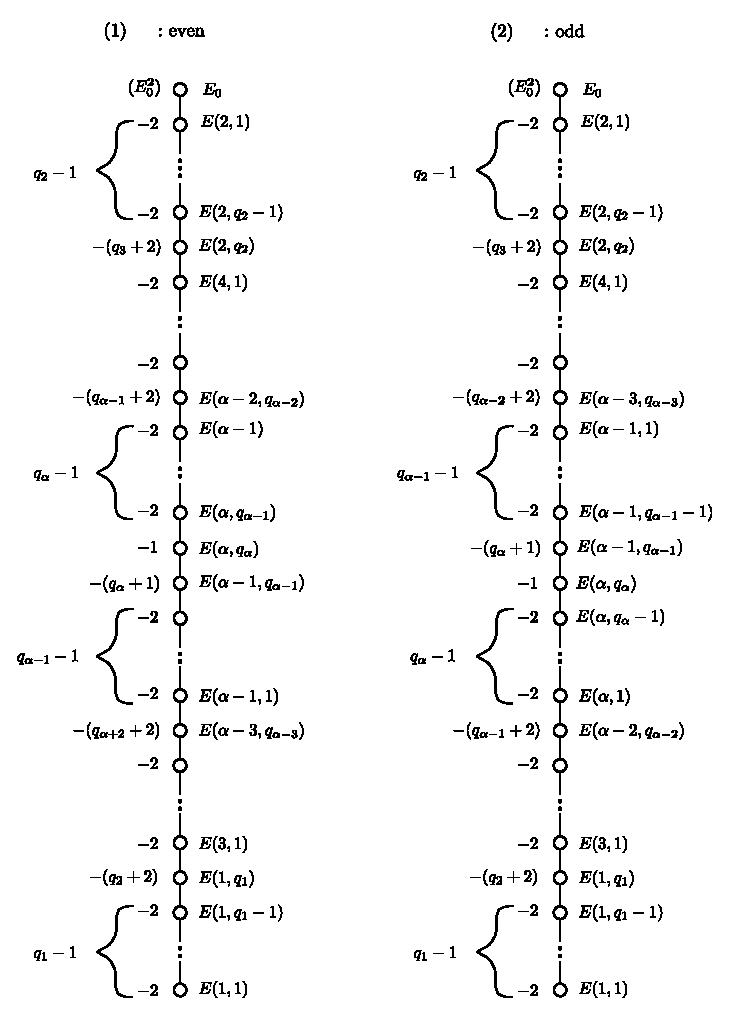
\includegraphics[scale=.9]{figures/chap2.add-fig1.eps}
    \end{figure}
    $\geqq d_{2}$\pageoriginale\ otherwise. More precisely, if $\alpha>1$
    and $q_{1}\geqq 2$, then $a(1,q_{1})>d_{0}$.
    
  \item If $\alpha\geqq 2$ then $a(s,q_{s})>d_{s-1}>d_{s}$ for $2\leqq
    s\leqq \alpha$. Especially, $a(\alpha,q_{\alpha})>d_{\alpha}$.
    
  \item For $2\leqq s\leqq \alpha$, $a(s,1)>a(s-1,q_{s-1})$.
    
  \item For $1\leqq s\leqq \alpha$ and $1\leqq t\leqq q_{s}-1$,
    $a(s,t+1)\geqq a(s,t)>0$.
    
  \item $d_{\alpha}|a(s,t)$.
    
  \item $a(\alpha,q_{\alpha})d_{\alpha}=d_{0}(d_{0}-d_{1})$.
  \end{enumerate}
\end{lemma*}

\begin{proof}
\begin{enumerate}
\renewcommand{\labelenumi}{(\theenumi)}
\item By definition,
  $a(l,q_{1})=q_{1}(d_{0}-d_{1})=q_{1}d_{0}-d_{0}+d_{2}=(q_{1}-1)d_{0}+d_{2}$. Since
  $d_{0}>d_{1}$ we have either $q_{1}\geqq 2$ or $q_{1}=1$ and
  $d_{2}>0$. If $q_{1}\geqq 2$ then $a(l,q_{1})\geqq d_{0}+d_{2}\geqq
  d_{0}$. If $q_{1}=1$ and $d_{2}>0$ then $a(l,q_{1})=d_{2}$. If
  $\alpha=1$ then $q_{1}\geqq 2$. Hence $a(l,q_{1})\geqq d_{0}$. If
  $\alpha\neq 1$ then $d_{2}\neq 0$ and $a(l,q_{1})\geqq d_{2}$. If
  $\alpha>1$ and $q_{1}\geqq 2$ then $a(l,q_{1})>d_{0}$.

\item If $\alpha\geqq 2$ then $a(l,q_{1})\geqq d_{2}$ by (1). Since
  $a(2,q_{2})=d_{0}+q_{2}(a(l,q_{1})-d_{2})$, we have $a(2,q_{2})\geqq
  d_{0}$. Hence $a(2,q_{2})>d_{1}>d_{2}$. If $\alpha\geqq 3$ we shall
  prove $a(s,q_{s})>d_{s-1}>d_{s}$ by induction on $s$. For $s=3$,
  $a(3,q_{3})=a(1,q_{1})+q_{3}(a(2,q_{2})-d_{3})>d_{2}+q_{3}(d_{2}-d_{3})>d_{2}$. By
  induction on $s(\geqq 4)$, assume that $a(s-2,q_{s-2})>d_{s-2}$ and
  $a(s-1,q_{s-1})>d_{s-1}$. Then
  $a(s,q_{s})=a(s-2,q_{s-2})+q_{s}(a(s-1,q_{s-1})-d_{s})>d_{s-2}+q_{s}(d_{s-1}-d_{s})>d_{s-2}>d_{s-1}$. Therefore,
  if $\alpha\geqq 2$, $a(s,q_{s})>d_{s-1}$ for $2\leqq s\leqq
  \alpha$. Especially $a(\alpha,q_{\alpha})>d_{\alpha-1}>d_{\alpha}$.

\item For $s=2$, $a(2,1)-a(1,q_{1})=d_{0}-d_{2}>0$. For $s\geqq 3$,
  $a(s,1)-a(s-1,q_{s-1})=a(s-2,q_{s-2})-d_{s}>0$ by (2).

\item For $s=1$, $a(1,t+1)-a(1,t)=d_{0}-d_{1}>0$. Thus
  $a(1,t+1)>a(1,t)>0$. For $s\geqq 2$,
  $a(s,t+1)-a(s,t)=a(s-1,q_{s-1})-d_{s}\geqq 0$, where\pageoriginale\
  $>0$ takes place if $s\geqq 3$. Thus $a(s,t+1)\geqq
  a(s,t)\geqq\ldots \geqq
  a(s,1)>a(s-1,q_{s-1})\geqq\ldots>a(1,q_{1})>0$ by (3). 

\item Note that $d_{\alpha}|d_{1},d_{2},\ldots,d_{\alpha}$. Since
  $a(1,t)=t(d_{0}-d_{1}),d_{\alpha}|a(1,t)$. Then
  $a(2,t)=d+t(a(1,q_{1})-d_{2})$, and $d_{\alpha}|a(2,t)$. Assume that
  $d_{\alpha}|a(s',t)$ for $s'<s$ and $1\leqq t\leqq q_{s'}$. Then
  $a(s,t)=a(s-2,q_{s-2})+t(a(s-1,q_{s-1})-d_{s})$, and
  $d_{\alpha}|a(s,t)$.

\item
  $a(\alpha,q_{\alpha})d_{\alpha}=a(\alpha-2,q_{\alpha-2})d_{\alpha}+a(\alpha-1,q_{\alpha-1})q_{\alpha}d_{\alpha}-q_{\alpha}d^{2}_{\alpha}$
\begin{align*}
&= a(\alpha-2,q_{\alpha-2})d_{\alpha} + \{a(\alpha-1,q_{\alpha-1}) -
  d_{\alpha}\}d_{\alpha-1} \\
&= a(\alpha-2,q_{\alpha-2})d_{\alpha} + \{a(\alpha-3,q_{\alpha-3})\\
  & \qquad +a(\alpha-2,q_{\alpha-2})q_{\alpha-1} -
  q_{\alpha-1}d_{\alpha-1}-d_{\alpha}\} d_{\alpha-1}\\
&=
  a(\alpha-2,q_{\alpha-2})(d_{\alpha}+q_{\alpha-1}d_{\alpha-1})+a(\alpha-3,q_{\alpha-3})d_{\alpha-1}-d_{\alpha-2}d_{\alpha-1}\\
&=
  a(\alpha-3,q_{\alpha-3})d_{\alpha-1}+\{a(\alpha-2,q_{\alpha-2})-d_{\alpha-1}\}d_{\alpha-2}. 
\end{align*}
Assume by induction that
$$
a(\alpha,q_{\alpha})d_{\alpha}=a(j-2,q_{j-2})d_{j}+\{a(j-1,q_{j-1})-d_{j}\}d_{j-1}.
$$
Then, since
$a(j-1,q_{j-1})-d_{j}=a(j-3,q_{j-3})+q_{j-1}a(j-2,q_{j-2})-q_{j-1}d_{j-1}-d_{j}=a(j-3,q_{j-3})+q_{j-1}a(j-2,q_{j-2})-d_{j-2}$,
we have
\begin{align*}
  a(\alpha,q_{\alpha})d_{\alpha} &=
  a(j-2,q_{j-2})(d_{j}+q_{j-1}d_{j-1})\\
  & \qquad +a(j-3,q_{j-3})d_{j-1}-d_{j-2}d_{j-1}\\
&= a(j-3,q_{j-3})d_{j-1}+\{a(j-2,q_{j-2})-d_{j-1}\}d_{j-2}.
\end{align*}
Thus,
$a(\alpha,q_{\alpha})d_{\alpha}=a_{0}d_{2}+\{a(1,q_{1})-d_{2}\}d_{1}=d_{0}d_{2}+(q_{1}-1)d_{0}d_{1}=d_{0}(d_{0}-d_{1})$.
\end{enumerate}
\end{proof}

\subsubsection{}\label{chap2:1.4.2}
Define positive integers $c(s,t)$ $(1\leqq s\leqq\alpha;1\leqq t\leqq
q_{s})$ inductively in the following way:
\begin{alignat*}{2}
c(1,t) & = t & \text{ \ for } 1\leqq t\leqq q_{1}\\
c(2,t) & = 1+tc(1,q_{1}) & \text{ \ for } 1\leq t\leq q_{2}\\
       &\qquad \ldots\ldots\ldots & \\
c(s,t) &= c(s-2,q_{s-2})+tc(s-1,q_{s-1}) & \text{ \  for } 1\leq t\leq
q_{s} \text{ and }\\ 
 & & 2\leqq s\leqq \alpha.
\end{alignat*}
With\pageoriginale\ the above notations, we shall show

\begin{lemma*}
$c(\alpha,q_{\alpha})d_{\alpha}=d_{0}$.
\end{lemma*}

\begin{proof}
$c(\alpha,q_{\alpha})d_{\alpha}=c(\alpha-2,q_{\alpha-2})d_{\alpha}+c(\alpha-1,q_{\alpha-1})q_{\alpha}d_{\alpha}$
\begin{align*}
&=
  c(\alpha-2,q_{\alpha-2})d_{\alpha}+c(\alpha-1,q_{\alpha-1})d_{\alpha-1}\\
&=
  c(\alpha-2,q_{\alpha-2})d_{\alpha}+\{c(\alpha-3,q_{\alpha-3})+c(\alpha-2,q_{\alpha-2})q_{\alpha-1}\}d_{\alpha-1}\\
&=
  c(\alpha-3,q_{\alpha-3})d_{\alpha-1}+c(\alpha-2,q_{\alpha-2})(d_{\alpha}+q_{\alpha-1}d_{\alpha-1})\\ 
&= c(\alpha-3,q_{\alpha-3})d_{\alpha-1}+c(\alpha-2,q_{\alpha-2})d_{\alpha-2}.
\end{align*}
As in the proof of Lemma \ref{chap2:1.4.1}, (6), we can show:
$$
c(\alpha,q_{\alpha})d_{\alpha}=c(j-2,q_{j-2})d_{j}+c(j-1,q_{j-1})d_{j-1}\quad\text{for}\quad
3\leqq j\leqq \alpha.
$$
Thus
$$
c(\alpha,q_{\alpha})d_{\alpha}=c(1,q_{1})d_{3}+c(2,q_{2})d_{2}=q_{1}d_{3}+(q_{1}q_{2}+1)d_{2}=d_{0}.
$$
\end{proof}

\subsection{}\label{chap2:1.5}
\begin{lemma*}
  Let $\mathscr{D}=\{V,X,C,\ell_{0},\Gamma,d_{0},d_{1},e\}$ be an
  admissible datum for $(X,C_{0})$ with $d_{0}>d_{1}\geqq 1$. Let
  $\rho:\widehat{V}\to V$ be the Euclidean transformation of $V$
  associated with $\mathscr{D}$. Let $\widehat{C}:=C^{(N)}=\rho'(C)$,
  $\widehat{\ell}_{0}:=\ell^{(N)}_{N}$, $\widehat{d}_{0}=d_{\alpha}$,
  and let
  $$
  \widehat{e}=\{a(\alpha,q_{\alpha})/d_{\alpha}+(e-1)c(\alpha,q_{\alpha})
  d_{0}/d_{\alpha}\}   
  $$
  and
  \begin{multline*}
  \widehat{\Gamma}  =e(d_{0}/d_{\alpha})E_{0}+\sum^{\alpha}_{s=1}
  \sum^{q_{s}}_{t=1} \{a(s,t)/d_{\alpha}+(e-1)c(s,t)d_{0}/d_{\alpha}\}\\
  E(s,t)+(d_{0}/d_{\alpha})\rho^{\ast}(\Gamma)-\widehat{e}\widehat{\ell}_{0}, 
  \end{multline*}
  where $a(s,t)$'s and $c(s,t)$'s are integers defined in \ref{chap2:1.4}. Let
  $\widehat{d}_{1}$ be the multiplicity of $\widehat{C}$ at
  $\widehat{P}_{0}:=\widehat{C}\cap \widehat{\ell}_{0}$. Then we have:
  \begin{enumerate}
    \renewcommand{\labelenumi}{\rm(\theenumi)}
  \item
    $\widehat{D}=\{\widehat{V},X,\widehat{C},\widehat{\ell}_{0},
    \widehat{\Gamma},\widehat{d}_{0},\widehat{d}_{1},\widehat{e}\}$  
    is an admissible datum for $(X,C_{0})$ with $\widehat{d}_{1}\leqq
    \widehat{d}_{0}\leqq d_{1}<d_{0}$ and $\widehat{e}\geqq 4e-2$. 

  \item $(\widehat{\ell}^{2}_{0})=-1$,\pageoriginale\ and
    $\widehat{\Gamma}$ contains 
    no exceptional components provided $\Gamma$ contains no exceptional
    components and $(\ell^{2}_{0})\neq q_{1}$ if $\alpha>1$ and
    $(\ell^{2}_{0})\neq q_{1}-1$ if $\alpha=1$.
    
  \item Let $\Lambda$ be the linear pencil on $\widehat{V}$
    spanned by $\widehat{C}$ and
    $\widehat{d}_{0}(\widehat{e}\widehat{\ell}_{0}+\widehat{\Gamma})$. Then
    $\Lambda$ is the proper transform by $\rho$ of the linear
    pencil $\Lambda$ on $V$ spanned by $C$ and $d_{0}(e\ell_{0}+\Gamma)$.
  \end{enumerate}
\end{lemma*}

\begin{proof}
By a straightforward computation we have
$$
C^{(N)}\sim
d_{0}E_{0}+\sum^{\alpha}_{s=1}\sum^{q_{s}}_{t=1}a(s,t)E(s,t)+d_{0}\Delta^{(N)}
$$
where
$\Delta^{(N)}=\rho^{\ast}((e-1)\ell_{0}+\Gamma)=(e-1)\{E_{0}+{\displaystyle{\mathop{\sum}^{\alpha}_{s=1}}\mathop{\sum}^{q_{s}}_{t=1}}c(s,t)E(s,t)+\rho^{\ast}(\Gamma)$
and where $(C^{(N)}\cdot\ell^{(N)}_{N})=d_{\alpha}$,
$(C^{(N)}\cdot\ell^{(N)}_{j})=0$ for $0\leqq j<N$ and $(C^{(N)}\cdot
\rho^{\ast}(\Gamma))=0$. Then, with $\widehat{C}$,
$\widehat{\ell}_{0}$, $\widehat{d}_{0}$, $\widehat{e}$ and
$\widehat{\Gamma}$ defined as above we have
$\widehat{C}\sim\widehat{d}_{0}(\widehat{e}\widehat{\ell}_{0}+\widehat{\Gamma})$. Note
that $\rho^{-1}(X)$ is identified with $X$, that
$\Supp(\widehat{\Gamma})=\overline{V-(X\cup \widehat{\ell}_{0})}$ as
is easily seen by Lemma \ref{chap2:1.4.1}, and that
$\widehat{V}-X=\widehat{\ell}_{0}\cup \widehat{\Gamma}$ satisfies the
condition (2) of Definition \ref{chap2:1.2.1}. Thus, we know that
$\widehat{\mathscr{D}}=\{\widehat{V},X,\widehat{C},\widehat{\ell}_{0},\widehat{\Gamma},\widehat{d}_{0},\widehat{d}_{1},\widehat{e}\}$
is an admissible datum for $(X,C_{0})$. It is clear that
$\widehat{d}_{1}\leqq \widehat{d}_{0}\leqq d_{1}<d_{0}$. Let
$d_{0}=b_{0}d_{\alpha}$ and $d_{1}=b_{1}d_{\alpha}$. Then
$(b_{0},b_{1})=1$ and $b_{0}>b_{1}\geqq 1$, whence $b_{0}\geqq
2$. Since $\widehat{e}=b_{0}(b_{0}-b_{1})+(e-1)b^{2}_{0}$ by virtue of
Lemmas \ref{chap2:1.4.1} and \ref{chap2:1.4.2}, we know that
$\widehat{e}\geqq 4(e-1)+2=4e-2$. The assertion (2) follows from Lemma
\ref{chap2:1.3.3}, and the assertion (3) is easy to prove.
\end{proof}

\subsection{}\label{chap2:1.6}
\begin{defi*}
  Let $\mathscr{D}=\{V,X,C,\ell_{0},\Gamma,d_{0},d_{1},e\}$ be an
  admissible datum for $(X,C_{0})$ with $d_{0}=d_{1}\geqq 1$. Let
  $P_{0}:=C\cap \ell_{0}$, and let $\sigma_{1}:V_{1}\to V_{0}:=V$ be the
  quadratic transformation of $V_{0}$ with\pageoriginale\ center at
  $P_{0}$. Let $C^{(1)}:=\sigma'_{1}(C)$, let
  $\ell_{1}:=\sigma^{-1}_{1}(P_{0})$ and let $P_{1}:=C^{(1)}\cap
  \ell_{1}$. Let $d^{(1)}_{1}$ be the multiplicity of $C^{(1)}$ at
  $P_{1}$. (Set $d^{(0)}_{1}:=d_{1}$). If
  $d_{0}=d^{(0)}_{1}=d^{(1)}_{1}$, let $\sigma_{2}:V_{2}\to V_{1}$ be
  the quadratic transformation of $V_{1}$ with center at $P_{1}$. Define
  $\sigma_{j}:V_{j}\to V_{j-1}$, $C^{(j)}$, $\ell_{j}:=\ell^{(j)}_{j}$,
  $\ell^{(j)}_{t}(0\leqq t<j)$ and $d^{(j)}_{1}$ inductively as follows
  when $1\leq j\leq e$ and
  $d_{0}=d^{(0)}_{1}=\ldots=d_{1}^{(j-1)}:\sigma_{j}$ is the quadratic
  transformation of $V_{j-1}$ with center at $P_{j-1}:=C^{(j-1)}\cap
  \ell_{j-1}$; $C^{(j)}:=\sigma'_{j}(C^{(j-1)})$,
  $\ell_{j}:=\sigma^{-1}_{j}(P_{j-1})$,
  $\ell^{(j)}_{t}:=\sigma'_{j}(\ell_{t}^{(j-1)})$; $d^{(j)}_{1}$ is the
  multiplicity of $C^{(j)}$ at $P_{j}:=C^{(j)}\cap \ell_{j}$. For
  $1\leqq i\leqq e$, if
  $d_{0}=d^{(0)}_{1}=d_{1}^{(1)}=\ldots=d_{1}^{(i-1)}$, defined the
  $(e,i)$-transformation $\rho$ of $V$ {\em associated with $\mathscr{D}$ (or
    simply, the $(e,i)$-transformation of $V$}) as the composition
  $\rho:=\sigma_{1}\ldots\sigma_{i}$. 
\end{defi*}

Here it should be noted that the Euclidean transformation of $V$
associated with $\mathscr{D}$ is defined when $d_{0}>d_{1}$, while the
$(e,i)$-transformation of $V$ is defined when
$d_{0}=d_{1}=d_{1}^{(1)}=\ldots=d_{1}^{(i-1)}$ and $1\leqq i\leqq e$.

\subsection{}\label{chap2:1.7}
\begin{lemma*}
  Let $\mathscr{D}=\{V,X,C,\ell_{0},\Gamma,d_{0},d_{1},e\}$ be an
  admissible datum for $(X,C_{0})$ with $d_{0}=d_{1}\geqq 1$. If the
  $(e,i)$-transformation $\rho:V_{i}\to V$ is defined for some $i$ with
  $1\leqq i\leqq e$ then we have the following:
  \begin{enumerate}
    \renewcommand{\labelenumi}{\rm(\theenumi)}
  \item $(\ell_{s}^{(i)}\cdot \ell^{(i)}_{t})=1$ if $t=s+1$ with $0\leqq
    s<i$; $(\ell^{(i)}_{s}\cdot \ell^{(i)}_{t})=0$ for other pairs
    $(s,t)$ with $s\neq t$.
    
  \item $((\ell^{(i)}_{0})^{2})=(\ell^{2}_{0})-1$,
    $((\ell^{(i)}_{t})^{2})=-2$ for $1\leqq t<i$ and
    $((\ell^{(i)}_{i})^{2})=-1$.
    
  \item
    $\mathscr{D}_{i}=\{V_{i},X,C^{(i)},\ell_{i},\Gamma_{i},d_{0},d^{(i)}_{1},(e-i)\}$
    is an admissible\pageoriginale\ datum for $(X,C_{0})$ when $1\leqq
    i<e$, where
    $$
    \Gamma_{i}:=\rho^{\ast}(\Gamma)+(e-i+1)\ell^{(i)}_{i-1}+\cdots+e\ell_{0}^{(i)}.
    $$
    If $(\ell^{2}_{0})\neq 0$ and $\Gamma$ contains no exceptional
    components then $\Gamma_{i}$ contains no exceptional components. The
    linear pencil $\Lambda^{(i)}$ on $V_{i}$ spanned by $C^{(i)}$ and
    $d_{0}((e-i)\ell_{i}+\Gamma_{i})$ is the proper transform by $\rho$ of
    the linear pencil $\Lambda$ on $V$ spanned by $C$ and
    $d_{0}(e\ell_{0}+\Gamma)$. 
    
  \item If $i=e$ we have $C^{(e)}\sim d_{0}\Gamma_{e}$, where
    $$
    \Gamma_{e}:=\rho^{\ast}(\Gamma)+\ell^{(e)}_{e-1}+\cdots+e\ell_{0}^{(e)}.
    $$
    The linear pencil $\Lambda^{(e)}$ on $V_{e}$ spanned by $C^{(e)}$ and
    $d_{0}\Gamma_{e}$ is the proper transform by $\rho$ of the linear
    pencil $\Lambda$ on $V$ spanned by $C$ and $d_{0}(e\ell_{0}+\Gamma)$;
    $\Lambda^{(e)}$ is irreducible and free from base points.
  \end{enumerate}
\end{lemma*}

\begin{proof}
(1) and (2) follow from a straightforward computation. (3) By a direct
  computation again we have for $1\leqq i\leqq e$:
$$
C^{(i)}\sim d_{0}\{(e-i)\ell_{i}+(e-i+1)\ell^{(i)}_{i-1}+\cdots+e\ell_{0}^{(i)}+\Gamma^{(i)}\}
$$
where $\Gamma^{(i)}:=\rho^{\ast}(\Gamma)$,
$(C^{(i)}\cdot\ell_{i})=d_{0}$, $(C^{(i)}\cdot\ell^{(i)}_{j})=0$ for
$0\leqq j<i$ and $(C^{(i)}\cdot \Gamma^{(i)})=0$. Note that
$\rho^{-1}(X)$ is identified with $X$, that
$V_{i}-\rho^{-1}(X)=\rho^{-1}(\Gamma)\cup \ell^{(i)}_{0}\cup
\ell^{(i)}_{1}\cup\ldots\cup\ell^{(i)}_{i}$ satisfies the condition
(2) of Definition \ref{chap2:1.2.1} and that
$\Supp(\Gamma_{i})=\overline{V_{i}-(X\cup \ell_{i})}$. Therefore, if
$1\leqq i<e$,
$\mathscr{D}_{i}=\{V_{i},X,C^{(i)},\ell_{i},\Gamma_{i},d_{0},d^{(i)}_{1},(e-i)\}$
is an admissible datum for $(X,C_{0})$. The other assertions are easy
to prove.

(4)~We have only to note that $\Lambda^{(e)}$ is irreducible. Since
$C^{(e)}$ is irreducible, $\Lambda^{(e)}$ is apparently
irreducible.
\end{proof}

\subsection{}\label{chap2:1.8}
We\pageoriginale\ need the following auxiliary

\begin{lemma*}
Let $k$ be an algebraically closed field of characteristic $p$ and let
$V$ be a nonsingular projective surface defined over $k$. Let $f:V\to
B$ be a surjective morphism of $V$ onto a nonsingular complete curve
$B$, whose general fibers are irreducible curves. Assume that we are
given a fiber $f^{\ast}(b)$ such that:
\begin{enumerate}
\renewcommand{\labelenumi}{\rm(\theenumi)}
\item $f^{\ast}(b)=d\Delta$, where $d$ is the multiplicity and
  $\Delta$ is the reduced form, \iec
  $f^{\ast}(b)={\displaystyle{\mathop{\sum}^{n}_{i=1}}}d_{i}\Delta_{i}$
  with irreducible components $\Delta_{i}$ then $d$ is the greatest
  common divisor of $d_{1},\ldots,d_{n}$ and
  $\Delta={\displaystyle{\mathop{\sum}^{n}_{i=1}}}(d_{i}/d)\Delta_{i}$,

\item
  $\Supp(\Delta)={\displaystyle{\mathop{\bigcup}^{n}_{i=1}}}\Delta_{i}$
  satisfies the following conditions;
\begin{enumerate}
\renewcommand{\theenumii}{\roman{enumii}}
\renewcommand{\labelenumii}{\rm(\theenumii)}
\item each irreducible component $\Delta_{i}$ is a nonsingular,
  rational complete curve,

\item $\Delta_{i}$ intersects $\Delta_{j}$ (if at all) transversely
  in at most one point,

\item $\Delta_{i}\cap \Delta_{j}\cap \Delta_{\ell}=\phi$ for three
  distinct indices,

\item $\Supp(\Delta)$ contains no cyclic chains.
\end{enumerate}
Then the multiplicity $d$ of $f^{\ast}(b)$ is a power of the
characteristic $p$.
\end{enumerate}
\end{lemma*}

\begin{proof}
Our proof consists of three steps.
\begin{enumerate}
\renewcommand{\theenumi}{\Roman{enumi}}
\renewcommand{\labelenumi}{\rm(\theenumi)}
\item Set $Z:=\Delta_{\red}$. We shall show that $Z$ is simply
  connected, \iec $Z$ has no nontrivial unramified covering of degree
  prime to $p$. Let $\varphi:W\to Z$ be an unramified covering of
  degree $m>1$ with $(m,p)=1$. For $1\leqq i\leqq n$,
  $\varphi_{i}:=\fprod{\varphi}{\Delta_{i}}{Z}:W_{i}:=\fprod{W}{\Delta_{i}}{Z}\to\Delta_{i}$
  is an unramified covering of $\Delta_{i}$. Since $\Delta_{i}$
  is\pageoriginale\ isomorphic to $\mathbb{P}^{1}$ and $\Delta_{i}$ is
  thus simply connected, $W_{i}$ is a disjoint union
  $W_{i}:=\Delta^{(1)}_{i}\cup\ldots\cup \Delta^{(m)}_{i}$ of
  irreducible components $\Delta^{(j)}_{i}(1\leqq j\leqq m)$ which are
  isomorphic to $\Delta_{i}$. Now we shall prove our assertion by
  induction on the number $n$ of irreducible components of $Z$. When
  $n=1$ our assertion holds clearly as seen from the above remark. For
  $n>1$ there exists an irreducible component of $Z$, say
  $\Delta_{1}$, such that $\Delta_{1}$ meets only one irreducible
  component of $Z$ other than $\Delta_{1}$ and
  $Z'=\overline{Z-\Delta_{1}}={\displaystyle{\mathop{\bigcup}^{n}_{i=2}}}\Delta_{i}$
  satisfies the same conditions (i) $\sim$ (iv) as above for $Z$. Let
  $P:=Z'\cap \Delta_{1}$ and let
  $\varphi':=\fprod{\varphi}{Z'}{Z}:W':=\fprod{W}{Z'}{Z}\to Z'$. Since
  $\varphi'$ is an unramified covering of degree $m$ we know by
  assumption of induction that $W$ is a disjoint union
  $W:={Z'}^{(1)}\cup\ldots\cup {Z'}^{(m)}$, where ${Z'}^{(j)}(1\leqq
  j\leqq m)$ is isomorphic to $Z'$. Let
  $\varphi^{-1}(P):=\{P^{(1)},\ldots,P^{(m)}\}$. We may assume with no
  loss of generality that $P^{(j)}\in {Z'}^{(j)}\cap \Delta^{(j)}_{1}$
  for $1\leqq j\leqq m$. Since $Z'$ and $\Delta_{1}$ meet
  transversely each other at $P$ and $\varphi$ is unramified,
  ${Z'}^{(j)}$ and $\Delta^{(j)}_{1}$ meet transversely each other at
  $P^{(j)}$ for $1\leqq j\leqq m$. Set
  $Z^{(j)}:={Z'}^{(j)}\cup\Delta^{(j)}_{1}$ for $1\leqq j\leqq
  m$. Then it is easy to see that each $Z^{(j)}$ is isomorphic to $Z$
  for $1\leqq j\leqq m$ and $W$ is a disjoint union of
  $Z^{(1)},\ldots,Z^{(m)}$. Thus, our assertion is proved.

\item Assume that $d$ is not a power of $p$, and write
  $d=p^{\alpha}d'$ with $(d',p)=1$. Let $t$ be a uniformisant of $B$
  at the point $b$, and let $B'$ be the complete nonsingular model of
  an algebraic function field $k(B)(t^{1/d'})$. The canonical morphism
  $\psi:B'\to B$ determined by the injection $k(B)\hookrightarrow
  k(B)(t^{1/d'})$ ramifies totally over the point\pageoriginale\
  $b$. Let $b'$ be the unique point of $B'$ over $b$. Let $V'$ be the
  normalization of $\fprod{V}{B'}{B}$ and let $\widehat{\psi}:V'\to V$
  and $f':V'\to B'$ be the canonical projections onto $V$ and $B'$,
  respectively. We have, thus, a commutative diagram:
\[
\xymatrix@=1.2cm{
V'\ar[d]^{f'}\ar[r]^{\widetilde{\psi}} & V\ar[d]^{f}\\
B'\ar[r]^{\psi} & B
}
\]
Let $W':={f'}^{\ast}(b')$. We shall show that $\widetilde{\psi}$ maps
$W'$ onto $p^{\alpha}\Delta$ (considered as a closed sub scheme of $V$)
and $\varphi':=\widetilde{\psi}|_{W'}:W'\to p^{\alpha}\Delta$ is a
nontrivial unramified covering of degree $d'$. Let $v$ be a
($k$-rational) point of $V$ on $\Delta$, and let $x$ be an element of
$\mathscr{O}_{V,v}$ such that $x=0$ is a local equation of $\Delta$
(considered as a divisor on $V$). Then we have $t=ux^{d}$ with $u\in
\mathscr{O}^{\ast}_{V,v}$. Hence we have
$t^{1/d'}=(u^{1/d'})x^{p^{\alpha}}$ in
$k(V'):=\foprod{k(V)}{k(B')}{k(B)}$. Here note that $t$ and $x$ cannot
be chosen so that $u$ has a $d'$-th root in $\mathscr{O}_{V,v}$;
indeed, if possible, $\foprod{k(V)}{k(B')}{k(B)}$ would be not an
integral domain, and this contradicts the fact that $k(V)$ is a
regular extension of $k(B)$. We have then:
\begin{align*}
\fprod{V'}{\Spec(\mathscr{O}_{V,v})}{V} &= \text{the normalization of
} \fprod{(\fprod{V}{B'}{B})}{\Spec(\mathscr{O}_{V,v})}{V}\\
&=\text{the normalization of }
\fprod{B'}{\Spec(\mathscr{O}_{V,v})}{B}\\
&= \Spec(\mathscr{O}_{V,v}[u^{1/d'}]).
\end{align*}
This implies that $\widetilde{\psi}:V'\to V$ is unramified at every
point of $V'$ over $v$. Moreover, we know by construction that
$\widetilde{\psi}^{\ast}(p^{\alpha}\Delta)={f'}^{\ast}(b')$
at\pageoriginale\ every point of $V'$ over $v$. Since these assertions
hold for all points $v$ of $\Delta$ we know that $\widetilde{\psi}$
maps $W'$ onto $p^{\alpha}\Delta$ and
$\varphi':=\widetilde{\psi}|_{W'}:W'\to p^{\alpha}\Delta$ is an
unramified covering of degree $d'$, where $\varphi'$ is nontrivial
because $W':={f'}^{\ast}(b')$ is connected.

\item Set $\varphi:\varphi'_{\red}$, $W:=W'_{\red}$ and
  $Z:=(p^{\alpha}\Delta)_{\red}$. Then $\varphi:W\to Z$ is a
  nontrivial unramified covering of degree $d'>1$, which contradict
  the assertion in step (I). Consequently, $d$ is a power of
  $p$.
\end{enumerate}
\end{proof}

\subsection{}\label{chap2:1.9}
As consequences of Lemma \ref{chap2:1.8} we have the following results.

\subsubsection{}\label{chap2:1.9.1}
\begin{coro*}
  Let $\mathscr{D}=\{V,X,C,\ell_{0},\Gamma,d_{0},d_{1},e\}$ be an
  admissible datum for $(X,C_{0})$ with $d_{0}=d_{1}>1$. Assume that
  $d_{0}$ is not divisible by $p$. Then there exists an admissible datum
  $\mathscr{D}'=\{V',X,C',\ell'_{0},\Gamma',d'_{0},d'_{1},e'\}$ for
  $(X,C_{0})$ such that:
  \begin{enumerate}
    \renewcommand{\labelenumi}{\rm(\theenumi)}
  \item $\mathscr{D}'$ is obtained from $\mathscr{D}$ by some
    $(e,i)$-transformation of $V$ associated with $\mathscr{D}$;
    
  \item $d'_{0}=d_{0}$, $d'_{1}<d'_{0}$ and $e'<e$;
    
  \item $({\ell'}^{2}_{0})=-1$, and $\Gamma'$ contains no exceptional
    components provided $(\ell^{2}_{0})\neq 0$ and $\Gamma$ contains no
    exceptional components.
  \end{enumerate}
\end{coro*}

\begin{proof}
\begin{enumerate}
\renewcommand{\theenumi}{\Roman{enumi}}
\renewcommand{\labelenumi}{\rm(\theenumi)}
\item Assume that
  $d_{0}=d_{1}=d_{1}^{(1)}=\ldots=d_{1}^{(i-1)}>d_{1}^{(i)}$ for some
  $i$ with $1\leqq i<e$. Let $\mathscr{D}_{i}$ be an admissible datum
  for $(X,C_{0})$ obtained from $\mathscr{D}$ by the
  $(e,i)$-transformation of $V$ associated with $\mathscr{D}$. Then
  $\mathscr{D}_{i}$ satisfies all conditions (1) $\sim$ (3) above by
  virtue of Lemma \ref{chap2:1.7}.

\item Assume that the equalities
  $d_{0}=d_{1}=d_{1}^{(1)}=\ldots=d_{1}^{(e-1)}$ hold. Let
  $\rho:V_{e}\to V$ be the $(e,e)$-transformation of $V$ associated
  with\pageoriginale\ $\mathscr{D}$, and let $\Delta:=\Gamma_{e}$. The
  linear pencil $\Lambda^{(e)}$ on $V_{e}$ spanned by $C^{(e)}$ and
  $d_{0}\Delta$ is an irreducible pencil free from base points. Hence
  $\Lambda^{(e)}$ defines a fibration $f:V_{e}\to \mathbb{P}^{1}_{k}$,
  of which $d_{0}\Delta$ is a multiple singular fiber because
  $d_{0}>1$. Note that $d_{0}$ is the multiplicity of the fiber
  $d_{0}\Delta$ by virtue of Lemma \ref{chap2:1.7} (esp. (4)) and that
  the irreducible components $\Delta_{i}$ of $\Delta$ (\iec
  $\Supp(\Delta)={\displaystyle{\mathop{\bigcup}^{n}_{i=1}}}\Delta_{i}$)
  satisfy the conditions (i) $\sim$ (iv) of Lemma \ref{chap2:1.8}. Hence,
  by virtue of Lemma \ref{chap2:1.8}, $d_{0}$ is a power of $p$, which
  contradicts the assumption that $d_{0}$ is not divisible by
  $p$.
\end{enumerate}
\end{proof}

\subsubsection{}\label{chap2:1.9.2}
\begin{coro*}
  Let $\mathscr{D}=\{V,X,C,\ell_{0},\Gamma,d_{0},d_{1},e\}$ be an
  admissible datum for $(X,C_{0})$ with $d_{0}=d_{1}\geqq 1$. Assume
  that the $(e,e)$-transformation $\rho:V_{e}\to V$ is defined, \iec the
  equalities $d_{0}=d_{1}=d^{(1)}_{1}=\ldots=d_{1}^{(e-1)}$ hold. Let
  $\Lambda$ be the linear pencil on $V$ spanned by $C$ and
  $d_{0}(e\ell_{0}+\Gamma)$. Then the generic member of $\Lambda$ has
  only one place outside of $X$, which is a purely inseparable place. In
  other words, a general member of $\Lambda$ has only one place outside
  of $X$.
\end{coro*}

\begin{proof}
\begin{enumerate}
\renewcommand{\theenumi}{\Roman{enumi}}
\renewcommand{\labelenumi}{\rm(\theenumi)}
\item Let $\Lambda^{(e)}$ be the proper transform of $\Lambda$ by
  $\rho$; $\Lambda^{(e)}$ is spanned by $C^{(e)}$ and $d_{0}\Lambda$,
  where $\Delta:=\Gamma_{e}$, and $\Lambda^{(e)}$ is an irreducible
  linear pencil free from base points. Set $\overline{S}:=\ell_{e}$
  (\cf \ref{chap2:1.7}). Then
  $(C^{(e)}\cdot\overline{S})=d_{0}(\Delta\cdot\overline{S})=d_{0}$,
  and $d_{0}$ is a power of $p$ in virtue of Lemma \ref{chap2:1.8}. Let
  $f:V_{e}\to \mathbb{P}^{1}_{k}$ be the fibration defined by
  $\Lambda^{(e)}$. Let $S:=\overline{S}-\{\overline{S}\cap \Delta\}$
  and $T:=\mathbb{P}^{1}_{k}-f(\Delta)$. Then, by restricting $f$ onto
  $S$ we have a surjective morphism $\varphi:S\to T$ of degree
  $d_{0}$. Choose inhomogeneous coordinates $s$ and $t$ on
  $S$\pageoriginale\ and $T$ respectively such that the point
  $C^{(e)}\cap S$ is defined by $s=0$ and the point $f(C^{(e)})$ is
  defined by $t=0$. Then $\varphi$ is given by a polynomial $t=G(s)$
  in $s$ with coefficient in $k$ and with $\deg G=d_{0}$. By choices
  of $s$ and $t$ we have $G(0)=0$. Since the point $C^{(e)}\cap S$ is
  a one-place point of $C^{(e)}$ and $\Lambda^{(e)}$ has no base
  points, we conclude readily that $G(s)$ is written as
  $G(s)=as^{d_{0}}$ with $a\in k$. We may assume that $a=1$ by
  substituting $s$ for $(a^{1/d}0)s$. This implies that
  $\overline{f}:=f|_{\overline{S}}:\overline{S}\to \mathbb{P}^{1}_{k}$
  is the $\alpha$-th iteration $F^{\alpha}$ of the Frobenius
  endomorphism $F$ of $\overline{S}$, where $d_{0}=p^{\alpha}$.

\item Let $K:=k(t)=k(\mathbb{P}^{1})$, and let $W$ be the generic
  fiber of $f$, \iec
  $W=\fprod{V^{(e)}}{\Spec(K)}{\mathbb{P}^{1}}$. Then $W$ is a
  projective normal curve defined over $K$, and the curve
  $\overline{S}$ gives rise to a point $\mathscr{P}$ on $W$ which is
  purely inseparable over $K$, as was seen in the step (I). Hence
  $\mathscr{P}$ is a one-place point of $W$. Thus the generic member
  of $\Lambda$ has only one place outside of $X$. 
\end{enumerate}
\end{proof}

The following example, which was communicated to the author by
$A$. Sathaye, shows that a general fiber of $\Lambda$ has only one place
outside of $X$, while some special fiber has 2 or more places outside
of $X$. Let $k$ be a field of characteristic $p>0$. Choose integers
$n$, $U$, $V$ such that (1) $UV=1+p+\cdots+p^{n}$ and (2) $U>V>1$ and
$LU-MV=1$ is the unique relation with $L$, $M>0$, $L<V$ and
$M<U$. Then there exists a unique positive integer a such that
$$
LUp^{n+1}+UV-1>aUV>LUp^{n+1}\quad\text{and}\quad a\not\equiv 0 \pmod{p}.
$$
Consider an affine plane curve $f(x,y)=x^{Vp}+y^{U_{p}}+x^{r}y^{s}$,
where $r=aV-Lp^{n+1}$ and\pageoriginale\ $s=Up-aU+Mp^{n+1}$. Then the
curve $f(x,y)$ has the property that $f+\lambda$ has exactly one place
at infinity for all except one value of $\lambda$ and for the special
value of $\lambda$, it has 2 or more places at infinity. Here $n$ can
be chosen to be $1$ for all $p\neq 2^{m}-1$ for any $m$, and $n\leqq
3$ otherwise. Consequently, $\deg f=Up<p^{2}$ in the former case and
$\deg f<p^{5}$ in the latter case.

\subsection{}\label{chap2:1.10}
\begin{coro*}[to Lemma \ref{chap2:1.5} and Corollary \ref{chap2:1.9.1}
  ]
  Let $\mathscr{D}=\{V,X,C,\ell_{0},\Gamma$, $d_{0},d_{1},e\}$ be an
  admissible datum for $(X,C_{0})$ such that at least one of $d_{0}$ and
  $d_{1}$ is not divisible by $p$. Then there exists an admissible datum
  $\widetilde{D}=\{\widetilde{V},X,\widetilde{C},\widetilde{\ell}_{0},
  \widetilde{\Gamma},1,1,\widetilde{e}\}$ 
  for $(X,C_{0})$ such that:
  \begin{enumerate}
    \renewcommand{\labelenumi}{\rm(\theenumi)}
  \item There exists a birational morphism $\rho:\widetilde{V}\to V$,
    which is the composition of Fuclidean transformations and the
    $(e,i)$-transfor\-mations associated with admissible data.
    
  \item $\widetilde{C}=\rho'(C)$ and $\rho^{-1}(X)\cong X$.
    
  \item The linear pencil $\widetilde{\Lambda}$ on $\widetilde{V}$
    spanned by $\widetilde{C}$ and
    $\widetilde{e}\widetilde{\ell}_{0}+\widetilde{\Gamma}$ is the proper
    transform by $\rho$ of the linear pencil $\Lambda$ on $V$ spanned by
    $C$ and $d_{0}(e\ell_{0}+\Gamma)$.
  \end{enumerate}
\end{coro*}

\begin{proof}
We shall prove the assertion by induction on $d_{0}$. If $d_{0}=1$, we
have only to take $\widetilde{\mathscr{D}}=\mathscr{D}$. If
$d_{0}>d_{1}$ then the Euclidean transformation $\rho_{0}$ of $V$
associated with $\mathscr{D}$ can be defined, and we obtain by Lemma
\ref{chap2:1.5} an admissible datum
$\widehat{\mathscr{D}}=\{\widehat{V},X,\widehat{C},\widehat{\ell}_{0},\widehat{\Gamma},\widehat{d}_{0},\widehat{d}_{1},\widehat{e}\}$
for $(X,C_{0})$ such that $\widehat{d}_{1}\leqq \widehat{d}_{0}\leqq
d_{1}<d_{0}$ and $\widehat{d}_{0}$ is not divisible by $p$. By
inductive assumption we have an admissible datum\pageoriginale\
$\widetilde{\mathscr{D}}=\{\widetilde{V},X,\widetilde{C},\widetilde{\ell}_{0},\widetilde{\Gamma},1,1,\widetilde{e}\}$
and a birational morphism $\rho_{0}:\widetilde{V}\to \widehat{V}$
which satisfy the above conditions (1) $\sim$ (3). Then we have only
to take $\widetilde{D}$ and $\rho:=\rho_{1}\rho_{0}$. If
$d_{0}=d_{1}>1$, Corollary \ref{chap2:1.9.1} shows that there exists an
admissible datum
$\mathscr{D}'=\{V',X,C',\ell'_{0},\Gamma',d'_{0},d'_{1},e'\}$ such
that $d'_{1}<d'_{0}=d_{1}=d_{0},d'_{0}$ is not divisible by $p$, and
that $\mathscr{D}'$ is obtained by some $(e,i)$-transformation $\rho'$
of $V$ associated with $\mathscr{D}$. By the former case treated above
we have an admissible datum $\widetilde{\mathscr{D}}$ and a birational
morphism $\rho_{2}:\widetilde{V}\to V'$ which satisfy the above
conditions (1) $\sim$ (3). Then we have only to take
$\widetilde{\mathscr{D}}$ and $\rho:=\rho_{2}\rho'$.
\end{proof}

\subsection{}\label{chap2:1.11}
\begin{lemma*}
  Let $\mathscr{D}=\{V,X,C,\ell_{0},\Gamma,1,1,e\}$ be an admissible
  datum for $(X,C_{0})$. Let $\rho:V_{e}\to V$ be the
  $(e,e)$-transformation of $V$ associated with $\mathscr{D}$, let
  $\Lambda^{(e)}$ be the linear pencil on $V_{e}$ spanned by $C^{(e)}$
  and
  $\Gamma_{e}=\rho^{\ast}(\Gamma)+\ell^{(e)}_{e-1}+\cdots+e\ell_{0}^{(e)}$
  {\em (\cf Lemma \ref{chap2:1.7})} and let $f:V_{e}\to \mathbb{P}^{1}_{k}$
  be the fibration defined by $\Lambda^{(e)}$. Then we have the
  following results:
  \begin{enumerate}
    \renewcommand{\labelenumi}{\rm(\theenumi)}
  \item $C^{(e)}$ is an irreducible curve which is nonsingular at
    $C^{(e)}\cap \ell_{e}$.
    
  \item $\ell_{e}$ is a cross-section of the fibration $f:V_{e}\to
    \mathbb{P}^{1}_{k}$. 
    
  \item $\Lambda^{(e)}$ has no multiple members.
    
  \item Let $D$ be a member of $\Lambda^{(e)}$ other than
    $\Gamma_{e}$. Then, $D$ is an irreducible curve; $D_{0}:=D\cap X$
    has only one place outside of $D_{0}$; if $C_{0}$ is nonsingular the
    arithmetic genus of $D$ is equal to the geometric genus of $C_{0}$.
    
  \item If $C_{0}$ is nonsingular and rational then $D$ is a
    non-singular rational curve; $X$ with a fibration
    $f_{0}:=f|_{X}:X\to
    \mathbb{A}^{1}_{k}:=\mathbb{P}^{1}_{k}-\{f(\Gamma_{e})\}$\pageoriginale\
    is an $\mathbb{A}^{1}$-bundle over $\mathbb{A}^{1}_{k}$, and hence
    $X$ is isomorphic to the affine plane $\mathbb{A}^{2}_{k}$. 
  \end{enumerate}
\end{lemma*}

\begin{proof}
It will be clear that the $(e,e)$-transformation $\rho:V_{e}\to V$
associated with $\mathscr{D}$ is defined. Lemma \ref{chap2:1.7} tells us
that $\Lambda^{(e)}$ is an irreducible pencil free from base
points. Hence the general fibers of $f$ are irreducible. Since
$(C^{(e)}\cdot\ell_{e})=1$ we know that $C^{(e)}$ is an irreducible
curve which is nonsingular at $C^{(e)}\cap \ell_{e}$ and that
$\ell_{e}$ is a cross-section of $f$. Hence $\Lambda^{(e)}$ has no
multiple members. Let $D$ be a member of $\Lambda^{(e)}$ other than
$\Gamma_{e}$. Then $(D\cdot \ell_{e})=1$. Since
$\overline{V_{e}-(X\cup \ell_{e})}=\Supp(\Gamma_{e})$ (\cf the proof
of Lemma \ref{chap2:1.7}) and since $X$ is affine, $D$ is an irreducible
member. Since $D_{0}=D-(D\cap \ell_{e})$ and $D\cap \ell_{e}$ is a
simple point of $D$, $D$ has only one place outside of $D_{0}$. By
invariance of arithmetic genera for members of a linear system we
have: $p_{a}(D)=p_{a}(C^{(e)})$, which is equal to the genus of
$C_{0}$ if $C_{0}$ is nonsingular. If $C_{0}$ is non-singular and
rational then $p_{a}(D)=0$, whence follows that $D$ is a nonsingular
rational curve and $D_{0}$ is isomorphic to the affine line
$\mathbb{A}^{1}_{k}$. Furthermore, if $C_{0}$ is nonsingular and
rational then $\varphi:V_{e}-\Supp(\Gamma_{e})\to
\mathbb{A}^{1}_{k}:=\mathbb{P}^{1}_{k}-\{f(\Gamma_{e})\}$ is a
$\mathbb{P}^{1}$-bundle over $\mathbb{A}^{1}_{k}$ by virtue of
Hironaka [22; Th.\@ 1.8] and $\ell_{e}-(\Gamma_{e}\cap \ell_{e})$ is a
cross-section of $\varphi$, where $\varphi$ is the restriction of $f$
onto $V_{e}-\Supp(\Gamma_{e})$. Hence, $f_{0}:=f|_{X}:X\to
\mathbb{A}^{1}_{k}$ is an $\mathbb{A}^{1}$-bundle over
$\mathbb{A}^{1}_{k}$, and $X$ is isomorphic to the affine plane
$\mathbb{A}^{2}_{k}$ because every $\mathbb{A}^{1}$-bundle over
$\mathbb{A}^{1}_{k}$ is trivial.
\end{proof}


\subsection{}\label{chap2:1.12}
Corollary \ref{chap2:1.10} combined with Lemma \ref{chap2:1.11} implies the
following 

\begin{theorem*}
Let\pageoriginale\
$\mathscr{D}=\{V,X,C,\ell_{0},\Gamma,d_{0},d_{1},e\}$ be an admissible
datum for $(X,C_{0})$ such that at least one of $d_{0}$ and $d_{1}$ is
not divisible by $p$, and let $\Lambda$ be the linear pencil on $V$
spanned by $C$ and $d_{0}(e\ell_{0}+\Gamma)$. Let $D$ be an arbitrary
member of $\Lambda$ other than $d_{0}(e\ell_{0}+\Gamma)$ and let
$D_{0}:=D\cap X$. Then we have the following:
\begin{enumerate}
\renewcommand{\labelenumi}{\rm(\theenumi)}
\item $D_{0}$ is an irreducible curve with only one place outside of
  $D_{0}$.

\item The geometric genus of $D$ is equal to the geometric genus of
  $C$ if $D$ is a general member of $\Lambda$ and $C_{0}$ is
  nonsingular.

\item If $C_{0}$ is nonsingular and rational $D_{0}$ is a nonsingular
  rational curve; $X$ is isomorphic to the affine plane
  $\mathbb{A}^{2}_{k}$.
\end{enumerate}
\end{theorem*}

\begin{proof}
By Corollary 1.10 there exist an admissible datum\break
$\widetilde{\mathscr{D}}=\{\widetilde{V},X,\widetilde{C},\widetilde{\ell}_{0},\widetilde{\Gamma},1,1,\widetilde{e}\}$
for $(X,C_{0})$ and a birational morphism $\rho:\widetilde{V}\to V$
such that the linear pencil $\widetilde{\Lambda}$ on $\widetilde{V}$
spanned by $\widetilde{C}$ and
$\widetilde{e}\widetilde{\ell}_{0}+\widetilde{\Gamma}$ is the proper
transform by $\rho$ of $\Lambda$. Let
$\widetilde{\rho}:\widetilde{V}(\widetilde{e})\to \widetilde{V}$ be
the $(\widetilde{e},\widetilde{e})$-transformation of $\widetilde{V}$
associated with $\widetilde{D}$ and let
$\widetilde{\Lambda}(\widetilde{e})$ be the proper transform of
$\widetilde{\Lambda}$ by $\widetilde{\rho}$. Let
$\sigma=\rho\widetilde{\rho}$. Then
$L:=\widetilde{\Lambda}(\widetilde{e})$ is the proper transform of
$\Lambda$ by $\sigma$. Let $D'$ be the member of $L$ corresponding to
$D$ of $\Lambda$. Then $D'_{0}:=D'\cap X$ is isomorphic to $D_{0}$,
where $X$ is identified with $\sigma^{-1}(X)$. The above assertions
now follow from the assertions (4) and (5) of Lemma
\ref{chap2:1.11}.
\end{proof}

\subsection{}\label{chap2:1.13}
\begin{lemma*}
  Let $\mathscr{D}$ and $\Lambda$ be as in Theorem \ref{chap2:1.12} and let
  $A=\Gamma(X,\mathscr{O}_{X})$. Then the following assertions hold.
  \begin{enumerate}
    \renewcommand{\labelenumi}{\rm(\theenumi)}
  \item Assume that $A$ is a factorial ring and that
    $A^{\ast}=k^{\ast}$. Let $f$ be a prime element of $A$ defining
    $C_{0}$, and let $C_{\alpha}$ be the curve\pageoriginale\ on $X$
    defined by $f-\alpha$ for $\alpha\in k$. Then $D_{0}$ {\em (\cf
      Theorem \ref{chap2:1.12})} coincides with $C_{\alpha}$ for some
    $\alpha\in k$, and conversely, every $C_{\alpha}$ is of the form
    $D_{0}$ for some member $D$ of $\Lambda$ other than
    $d_{0}(e\ell_{0}+\Gamma)$. 
    
  \item If $C_{0}$ is nonsingular and rational then $A$ is a polynomial
    ring in two variables over $k$; thence $A$ is a factorial ring with
    $A^{\ast}=k^{\ast}$. 
  \end{enumerate}
\end{lemma*}

\begin{proof}
\begin{enumerate}
\renewcommand{\labelenumi}{(\theenumi)}
\item Under the assumptions of the assertion (1) we have
  $(f)=C-\Delta$ with a divisor $\Delta$ such that
  $\Supp(\Delta)\subset \ell_{0}\cup \Supp(\Gamma)$. Let $g$ be an
  element of $k(V)$ such that $(g)=C-d_{0}(e\ell_{0}+\Gamma)$. Then
  $(f/g)=d_{0}(e\ell_{0}+\Gamma)-\Delta$, whence $f/g$ is an
  invertible element of $A$. Since $A^{\ast}=k^{\ast}$, $f=\lambda g$
  with $\lambda\in k^{\ast}$. Hence
  $(f)=C-d_{0}(e\ell_{0}+\Gamma)$. This implies that $\Lambda$ is
  spanned by $1$ and $f$ (or more precisely, by
  $d_{0}(e\ell_{0}+\Gamma)$ and $d_{0}(e\ell_{0}+\Gamma)+(f)$. It is
  now clear that the assertion (1) holds.

\item The second assertion was proved in the assertion (3) of Theorem
  \ref{chap2:1.12}.
\end{enumerate}
\end{proof}

\subsection{}\label{chap2:1.14}
\begin{theorem*}
  Let $A$ be a nonsingular, rational, affine $k$-domain of dimension
  $2$, and let $X:=\Spec(A)$. Assume that the following conditions hold:
  \begin{enumerate}
    \renewcommand{\labelenumi}{\rm(\theenumi)}
  \item There exists an irreducible closed curve $C_{0}$ on $X$, which
    is isomorphic to the affine line $\mathbb{A}^{1}$ over $k$.
    
  \item There exists an admissible datum
    $\mathscr{D}=\{V,X,C,\ell_{0},\Gamma,d_{0},d_{1},e\}$ for
    $(X,C_{0})$ such that at least one of $d_{0}$ and $d_{1}$ is not
    divisible by $p$.
  \end{enumerate}
  Then $X$ is isomorphic to the affine plane $\mathbb{A}^{2}$ over
  $k$. Furthermore if\pageoriginale\ $f$ is an element of $A$ defining
  the curve $C_{0}$ then $A=k[f,g]$ for some element $g$ of $A$.
\end{theorem*}

\begin{proof}
The first assertion was proved in Theorem \ref{chap2:1.12}. We shall show
the second assertion. By virtue of Lemma \ref{chap2:1.13}, the proof of
Theorem \ref{chap2:1.12} and Lemma \ref{chap2:1.11}, we know that $X$ has a
structure of an $\mathbb{A}^{1}$-bundle over
$\mathbb{A}^{1}_{k}:=\Spec(k[f])$, whose fibers are the curves
$C_{\alpha}$ defined by $f-\alpha$ with $\alpha\in k$. Hence
$A=k[f,g]$ for some element $g$ of $A$.
\end{proof}

\subsection{}\label{chap2:1.15}
\noindent \textbf{Proof of Irreducibility theorem.} 
Set $X:=\mathbb{A}^{2}=\Spec(k[x,y])$. Then, as seen in \ref{chap2:1.2.2},
$\mathscr{D}_{0}=\{\mathbb{P}^{2}_{k},X,C,\ell_{0},\phi,d_{0},d_{1},1\}$
is an admissible datum for $(X,C_{0})$; (for the notations, see the
paragraph \ref{chap2:1.1}). We may assume that $d_{0}>1$; if otherwise, $C$
is a line on $\mathbb{P}^{2}_{k}$ and the assertion of the theorem is
apparently true. If $d_{0}>1$, the theorem follows from Theorem
\ref{chap2:1.12} and Lemma \ref{chap2:1.13}.

\subsection{}\label{chap2:1.16}
\noindent \textbf{Proof of Generic irreducibility theorem.} 
Let $\mathscr{D}_{0}$ be as in \ref{chap2:1.15}; we may assume that
$d_{0}>d_{1}$. Starting with the Euclidean transformation of
$\mathbb{P}^{2}_{k}$ associated with $\mathscr{D}_{0}$ and repeating
successively the Euclidean transformations or the
$(e,i)$-transformations associated with admissible data we obtain
ultimately an admissible datum
$\mathscr{D}=\{V,X,C,\ell_{0},\Gamma,d_{0},d_{1},e\}$ such that one of
the following conditions holds:
\begin{enumerate}
\renewcommand{\labelenumi}{(\theenumi)}
\item $d_{0}=d_{1}=1$; 

\item $d_{0}=d_{1}>1$ and $e=1$.
\end{enumerate}
In the case (1), we know by virtue of Lemma \ref{chap2:1.11} that every
curve $C_{\alpha}(\alpha\in k)$ is an irreducible curve with only one
place at infinity. In\pageoriginale\ the case (2), the generic
irreducibility theorem follows from Corollary \ref{chap2:1.9.2}.

\subsection{}\label{chap2:1.17}
\noindent \textbf{Proof of the Embedding theorem.} 
Consider an admissible datum $\mathscr{D}_{0}$ in the paragraph
\ref{chap2:1.15}. If $d_{0}=1$ the theorem holds apparently; hence we may
assume that $d_{0}>1$. Then $d_{0}>d_{1}\geqq 1$. Now the embedding
theorem follows from Theorem \ref{chap2:1.14}.

\section{Linear pencils of rational curves}\label{chap2:sec2}\pageoriginale\

\subsection{}\label{chap2:2.1}
In this section the ground field $k$ is assumed to be an algebraically
closed field of characteristic $p$. Let $V$ be a non-singular
projective surface defined over $k$. We shall consider an irreducible
linear pencil $\Lambda$ on $V$ satisfying the properties:
\begin{enumerate}
\renewcommand{\labelenumi}{\rm(\theenumi)}
\item {\em General members of $\Lambda$ are rational curves.}

\item {\em The generic member of $\Lambda$ is smoothable; namely,
  setting $\mathscr{K}:=$ the sub field of $k(V)$ corresponding to the
  pencil $\Lambda$, the complete normal $\mathscr{K}$-model of an
  algebraic function field $k(V)$ in one variable over $\mathscr{K}$
  is geometrically regular over $\mathscr{K}$.} The property (2) is
  equivalent to saying:

\renewcommand{\labelenumi}{\rm(\theenumi$'$)}
\setcounter{enumi}{1}
\item {\em There exist a nonsingular projective surface
  $\widetilde{V}$ and a birational morphism $\rho:\widetilde{V}\to V$
  such that general members of the proper transform
  $\widetilde{\Lambda}$ of $\Lambda$ by $\rho$ are nonsingular curves.}
\end{enumerate}
When the field $k$ is of characteristic zero the pencil $\Lambda$
satisfies automatically the property (2); hence the condition (2) is
superfluous. Moreover, we note by Tsen's Theorem that $V$ is a
rational surface if $\Lambda$ has the properties (1) and (2). In the
next chapter we shall consider a linear pencil having only the
property (1) but not (2), in order to construct unirational,
irrational surfaces.

\subsection{}\label{chap2:2.2}
\begin{lemma*}
  Let $f:V\to B$ be a surjective morphism from a nonsingular projective
  surface $V$ onto a nonsingular complete curve $B$ such that almost all
  fibers are isomorphic to $\mathbb{P}^{1}_{k}$. Let
  $F=n_{1}C_{1}+\cdots+n_{r}C_{r}$ be a singular fiber of $f$, where
  $C_{i}$ is an irreducible curve,\pageoriginale\ $C_{i}\neq C_{j}$ if
  $i\neq j$, and $n_{i}>0$. Then we have:
  \begin{enumerate}
    \renewcommand{\labelenumi}{\rm(\theenumi)}
  \item The greatest common divisor $(n_{1},\ldots,n_{r})$ of
    $n_{1},\ldots,n_{r}$ is 1;\break  
    $\Supp(F)={\displaystyle{\mathop{\bigcup}^{r}_{i=1}}}C_{i}$ is
    connected.
    
  \item For $1\leqq i\leqq r$, $C_{i}$ is isomorphic to
    $\mathbb{P}^{1}_{k}$ and $(C^{2}_{i})<0$.
    
  \item For $i\neq j$, $(C_{i}\cdot C_{j})=0$ or $1$.
    
  \item For three distinct indices $i$, $j$ and $\ell$, $C_{i}\cap
    C_{j}\cap C_{\ell}=\phi$.
    
  \item One of $C_{i}$'s, say $C_{1}$, is an exceptional component, \iec
    an exceptional curve of the first kind. If $\tau:V\to V_{1}$ is the
    contraction of $C_{1}$, then $f$ factors as
    $f:V\xrightarrow{\tau}V_{1}\xrightarrow{f_{1}}B$, where
    $f_{1}:V_{1}\to B$ is a fibration by $\mathbb{P}^{1}$.
    
  \item If one of $n_{i}$'s, say $n_{1}$, equals $1$ then there is an
    exceptional component among $C_{i}$'s with $2\leqq i\leqq n$.
  \end{enumerate}
\end{lemma*}

\begin{proof}[See Gizatullin \cite{16}]
\begin{enumerate}
\renewcommand{\theenumi}{\Roman{enumi}}
\renewcommand{\labelenumi}{(\theenumi)}
\item Let $m=(n_{1},\ldots,n_{r})$ and let $C=mD$ with
  $D:=(n_{1}/m)C_{1}+\cdots +(n_{r}/m)C_{r}$. Then, by the arithmetic
  genus formula we have:
$$
p_{a}(C)=\{m^{2}(D^{2})+m(D\cdot K_{V})\}/2+1=m(D\cdot K_{V})/2+1=0.
$$
Since $(D\cdot K_{V})$ is an integer, either $m=1$ or $m=2$ and
$(D\cdot K_{V})=-1$. In the latter case, $p_{a}(D)=\{(D^{2})+(D\cdot
K_{V})\}2+1=1/2$, which is a contradiction. Hence $m=1$. If $r=1$ then
$C$ is isomorphic to $\mathbb{P}^{1}_{k}$. Hence $r\geqq 2$ and we
know by virtue of Zariski's connectedness theorem that
$\Supp(F)={\displaystyle{\mathop{\bigcup}^{r}_{i=1}}}C_{i}$ is
connected.

\item For each $i$,
  $n_{i}(C^{2}_{i})+{\displaystyle{\mathop{\sum}_{i\neq
      j}}}n_{j}(C_{i}\cdot C_{j})=0$ where $(C_{i}\cdot C_{j})>0$ for
  some $j$ because $F$ is connected. Hence $(C^{2}_{i})<0$. To prove
  the\pageoriginale\ assertions (2), (3), (4) and (5) we have only to
  show that one of $C_{i}$'s is an exceptional component. Note that
  $(F\cdot K_{V})=-2$ because $p_{a}(F)=0$. Hence we have:
\begin{equation*}
-2=(F\cdot K_{V})=\sum_{i}n_{i}(C_{i}\cdot
K_{V})=\sum_{i}n_{i}(2p_{a}(C_{i})-2-(C^{2}_{i})),\tag{$\ast$}
\end{equation*}
where $2p_{a}(C_{i})-2-(C^{2}_{i})\geqq -1$ and the equality holds if
and only if $C_{i}$ is an exceptional curve of the first
kind. However, it is impossible that $2p_{a}(C_{i})-2-(C^{2}_{i})\geqq
0$ for every $i$, as seen from the above equality $(\ast)$. Therefore,
$2p_{a}(C_{i})-2-(C^{2}_{i})=-1$ for some $i$. 

\item We shall prove the assertion (6). Assume the contrary, \iec
  $C_{1}$ is an exceptional component with $n_{1}=1$ and none of
  $C_{i}$'s $(2\leqq i\leqq r)$ is an exceptional component. Then we
  have:
$$
2p_{a}(C_{1})-2-(C^{2}_{1})=-1~\text{and}~
2p_{a}(C_{i})-2-(C^{2}_{i})\geqq 0~\text{for}~ 2\leqq i\leqq r.
$$
Then we have
${\displaystyle{\mathop{\sum}_{i}}}n_{i}(2p_{a}(C_{i})-2-(C^{2}_{i}))\geqq
-1$, which contradicts the equality $(\ast)$.
\end{enumerate}
\end{proof}

\subsection{}\label{chap2:2.3}
\begin{lemma*}
  Let $V$ be a nonsingular projective surface and let $\Lambda$ be an
  irreducible linear pencil on $V$ satisfying the properties $(1)$ and
  $(2)$ of \ref{chap2:2.1}. Let $B$ be the set of points of $V$ which are base
  points of $\Lambda$. Let $F:=n_{1}C_{1}+\cdots+n_{r}C_{r}$ be a
  reducible member of $\Lambda$ such that $r\geqq 2$, where $C_{i}$ is
  an irreducible component, $C_{i}\neq C_{j}$ if $i\neq j$, and
  $n_{i}>0$. Then the following assertions hold:
  \begin{enumerate}
    \renewcommand{\labelenumi}{\rm(\theenumi)}
  \item If $C_{i}\cap B=\phi$ then $C_{i}$ is isomorphic to
    $\mathbb{P}^{1}_{k}$ and $(C^{2}_{i})<0$.
    
  \item If $C_{i}\cap C_{j}\neq \phi$ for $i\neq j$ and $C_{i}\cap
    C_{j}\cap B=\phi$ then $C_{i}\cap C_{j}$\pageoriginale\ consists of a
    single point 
    where $C_{i}$ and $C_{j}$ intersect each other transversely.
    
  \item For three distinct indices $i$, $j$, $\ell$, if $C_{i}\cap
    C_{j}\cap C_{\ell}\cap B=\phi$ then $C_{i}\cap C_{j}\cap
    C_{\ell}=\phi$.
    
  \item Assume that $(C^{2}_{i})<0$ whenever $C_{i}\cap B\neq
    \phi$. Then the set $S=\{C_{i};C_{i}$ is an irreducible component of
    $F$ such that $C_{i}\cap B=\phi\}$ is nonempty, and there is an
    exceptional component in the set $S$.
    
  \item With the same assumption as in $(4)$ above, if a component of
    $S$, say $C_{1}$, has multiplicity $n_{1}=1$ then there exists an
    exceptional component in $S$ other than $C_{1}$.
  \end{enumerate}
\end{lemma*}

\begin{proof}
Let $\rho:\widetilde{V}\to V$ be the (shortest) succession of
quadratic transformations with centers at base points (including
infinitely near base points) of $\Lambda$ such that the proper
transform $\widetilde{\Lambda}$ of $\Lambda$ by $\rho$ has no base
points. Then, by the equivalence of the properties (2) and $(2')$ as
explained in \ref{chap2:2.1}, general members of $\widetilde{\Lambda}$ are
isomorphic to $\mathbb{P}^{1}_{k}$. The assertions (1), (2) and (3)
are then apparently true. We shall prove the assertions (4) and (5),
assuming that $B\neq \phi$. Let $P\in B$. Set $P_{0}:=P$, and let
$P_{1},\ldots,P_{s-1}$ exhaust infinitely near base points of
$\Lambda$ such that $P_{i}$ is an infinitely near point of $P_{i-1}$
of order one for $1\leqq i\leqq s-1$. For $1\leqq i\leqq s$, let
$\sigma_{i}:V_{i}\to V_{i-1}$ be a quadratic transformation of
$V_{i-1}$ with center at $P_{i-1}$, where $V_{0}:=V$, and let
$\sigma=\sigma_{1}\ldots\sigma_{s}$. Then $\sigma$ factors $\rho$,
\iec $\rho=\sigma\cdot \overline{\rho}$. Let
$E'_{i}:=(\sigma_{i+1}\ldots\sigma_{s})'(\sigma^{-1}_{i}(P_{i-1}))$
for $1\leqq i<s$ and let $E'_{s}:=\sigma^{-1}_{s}(P_{s-1})$. Let
$E_{i}:=\overline{\rho}'(F'_{i})$ for $1\leqq i\leqq s$. It is clear
that $E'_{i}\cong E_{i}$ and $({E'}^{1}_{i})=(E^{2}_{i})$ for $1\leq
i\leqq s$,\pageoriginale\  and that $(E^{2}_{i})<-1$ for $1\leqq i<s$
and $(E^{2}_{s})=-1$. Moreover $E_{s}$ is not contained in any member
of $\widehat{\Lambda}$; indeed, if otherwise, $\widetilde{\Lambda}$
would have yet a base point on $E_{s}$, which contradicts the choice
of points $P_{1},\ldots,P_{s-1}$. The member $\widetilde{F}$ of
$\widetilde{\Lambda}$ corresponding to $F$ of $\Lambda$ may contain
some (not necessarily all) of $E_{1},\ldots,E_{s-1}$. After the above
argument made for every point of $B$ we know that if we write
$\widetilde{F}=(n_{1}\widetilde{C}_{1}+\cdots+n_{r}\widetilde{C}_{r})+(m_{1}D_{1}+\cdots+m_{t}D_{t})$
with $\widetilde{C}_{i}=\rho'(C_{i})$ for $1\leqq i\leqq r$ then we
have;
\begin{itemize}
\item[$1^{\circ}$] if $C_{i}\in S$ then $\widetilde{C}_{i}\cong C_{i}$
    and $(\widetilde{C}^{2}_{i})=(C^{2}_{i})$,

\item[$2^{\circ}$] if $C_{i}\not\in S$ then
  $(\widetilde{C}^{2}_{i})\leqq -2$,

\item[$3^{\circ}$] $(D^{2}_{i})\leqq -2$ for $1\leqq i\leqq t$.
\end{itemize}
Then the assertions (4) and (5) follow from the assertions (5) and (6)
of Lemma \ref{chap2:2.2}.
\end{proof}

\subsection{}\label{chap2:2.4}
Let $\mathbb{A}^{2}_{k}:=\Spec(k[x,y])$ be the affine plane, and fix
an open immersion of $\mathbb{A}^{2}_{k}$ into $\mathbb{P}^{2}_{k}$ as
the complement of a line $\ell_{0}$\footnote{We note that if
  $\mathbb{A}^{2}_{k}$ is embedded into $\mathbb{P}^{2}_{k}$ as an
  affine open set then the complement is a line. Indeed, let
  $\tau:\mathbb{A}^{2}_{k}\to \mathbb{P}^{2}_{k}$ be such an
  embedding; then
  $\mathbb{P}^{2}_{k}-\tau(\mathbb{A}^{2}_{k})=\cup^{r}_{i=1}C_{i}$
  with irreducible components $C_{i}$. If $r=1$, $C_{1}\sim m_{1}H$
  where $H$ is a line of $\mathbb{P}^{2}_{k}$. Since
  $\Pic(\mathbb{A}^{2}_{k})=(0)$ we have $m=1$. Assume that $r\geqq 2$
and $C_{i}\sim m_{i}H$ for $1\leqq i\leq r$. Then there exists a
nonconstant regular function $f$ on $(\mathbb{A}^{2}_{k})$ such that
$(f)=m_{1}C_{2}-m_{2}C_{1}$, which is a contradiction.}. Let $f$
$k[x,y]$ be an irreducible element such that the curve $C_{0}$ defined
by $f=0$ is a nonsingular, rational curve. Let $C$ be the closure of
$C_{0}$ in $\mathbb{P}^{2}_{k}$, and let $d:=(C\cdot\ell_{0})$. Denote
by $\Lambda(f)$ the linear pencil on $\mathbb{P}^{2}_{k}$ spanned by
$C$ and $d\ell_{0}$; $\Lambda(f)$ is an irreducible pencil determined
uniquely by the inclusion $k(f)\hookrightarrow
k(x,y)$. We\pageoriginale\ may ask under what conditions the pencil
$\Lambda(f)$ has properties (1) and (2) of the paragraph \ref{chap2:2.1}.

\subsubsection{}\label{chap2:2.4.1}
\begin{lemma*}
  With the above notations, the pencil $\Lambda(f)$ has properties $(1)$
  and $(2)$ of \ref{chap2:2.1} if and only if $f$ is a field generator, \iec
  there exists an element $g$ of $k(x,y)$ such that $k(x,y)=k(f,g)$.
\end{lemma*}

\begin{proof}
The properties (1) and (2) of \ref{chap2:2.1} are equivalent to saying that
an algebraic function field $k(x,y)$ in one variable over $k(f)$ has
genus $0$. By vartue of Tsen's theorem, this is equivalent to saying
that $k(x,y)$ is a purely transcendental extension of $k(f)$.
\end{proof}

\subsubsection{}\label{chap2:2.4.2}
Various properties of a field generator were studied by Russel
\cite{48}, \cite{50}, one of which tells us:

\begin{lemma*}[Russell [48; Cor. 3.7] ]
Let $f\in k[x,y]$ be a field generator. Then there are at most two
points (including infinitely near points) of $f$ on the line at
infinity. In particular, the degree form of $f$ has at most two
distinct irreducible factors.
\end{lemma*}

\subsubsection{}\label{chap2:2.4.3}
If the curve $C_{0}$ defined by $f=0$ is isomorphic to
$\mathbb{A}^{1}_{k}$, the pencil $\Lambda(f)$ satisfies the properties
(1) and (2) of \ref{chap2:2.1} under some mild restrictions, as we saw in
the previous section. An example of a nonsingular, rational curve
$C_{0}:f=0$, for which $\Lambda(f)$ does not satisfy the properties
(1) and (2) of \ref{chap2:2.1}, is given by the following:

\begin{example*}
Assume that $p\neq 2$. Let $f:=xy^{2}(x+y)+2xy+1$. Then
$f$\pageoriginale\ is an irreducible element and the curve $C_{0}:f=0$
is a non-singular, rational curve. Moreover, if $\rho:\widetilde{V}\to
\mathbb{P}^{2}_{k}$ is the shortest succession of quadratic
transformations such that the proper transform $\widetilde{\Lambda}$
of $\Lambda(f)$ by $\rho$ has no base points, then
$\widetilde{\Lambda}$ is a pencil of elliptic curves with three
singular fibers and $\widetilde{\Lambda}$ has the following
configuration:
\begin{figure}[H]
\centering
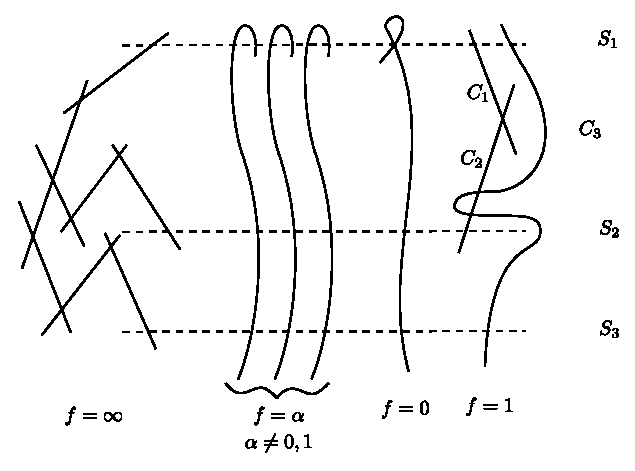
\includegraphics[scale=.8]{figures/chap2-fig1.eps}
\end{figure}
\noindent
where;
\begin{enumerate}
\itemsep=3pt
\renewcommand{\labelenumi}{\theenumi$^{\circ}$}
\item two dotted lines $S_{2}$ and $S_{3}$ are cross-sections of
  $\widetilde{\Lambda}$; and the dotted line $S_{1}$ meets each fiber
  of $\widetilde{\Lambda}$ with multiplicity $2$;  


\item the singular fiber $f=\infty$ is a singular fiber of type
  $B_{9}$ (\cf \v{S}afarevi\v{c} [51; p.\@ 172]);

\item the singular fiber $f=0$ is a rational curve with only one
  (ordinary) node on the line $S_{1}$;

\item the singular fiber $f=1$ has three irreducible components
  $C_{1}$, $C_{2}$ and $C_{3}$ which are nonsingular rational curves,
  and correspond to the curves $y=0$, $x=0$ and $y^{2}+xy+2=0$
  respectively, in the decomposition\pageoriginale\
  $f-1=yx (y^{2}+xy+2)$; $(C^{2}_{1})=-1$, $(C^{2}_{2})=-3$ and
  $(C^{2}_{3})=-2$; 

\item each fiber $f=\alpha(\alpha\in k, \alpha\neq 0,1)$ is a
  nonsingular elliptic curve meeting $S_{1}$ in two distinct points;

\item $\widetilde{V}$-(the fiber $f=\infty)\cup S_{1}\cup S_{2}\cup
  S_{3}\cong \mathbb{A}^{2}_{k}$.
\end{enumerate}
\end{example*}

\subsubsection{}\label{chap2:2.4.4}
Let $f\in k[x,y]$ be an irreducible element such that the curve
$C_{0}:f=0$ is a nonsingular rational curve. Even if $C_{0}$ has
exactly two places at infinity and $f$ is a field generator, a curve
$C_{\alpha}:f=\alpha(\alpha\in k)$ does not necessarily have two
places at infinity as is shown by the next:

\begin{example*}
Assume that $p\neq 2$. Let $f=x^{2}y^{2}+2xy^{2}+y^{2}+2xy+1$. Then
$f$ is an irreducible element and the curve $C_{0}:f=0$ is a
nonsingular rational curve. Moreover, if
$\rho:\widetilde{V}\to\mathbb{P}^{2}_{k}$ is the shortest succession
of quadratic transformations such that the proper transform
$\widetilde{\Lambda}$ of $\Lambda(f)$ has no base points, then
$\widetilde{\Lambda}$ is a pencil of rational curves with two singular
fibers and $\widetilde{\Lambda}$ has the following configuration:
\begin{figure}[H]
\centering
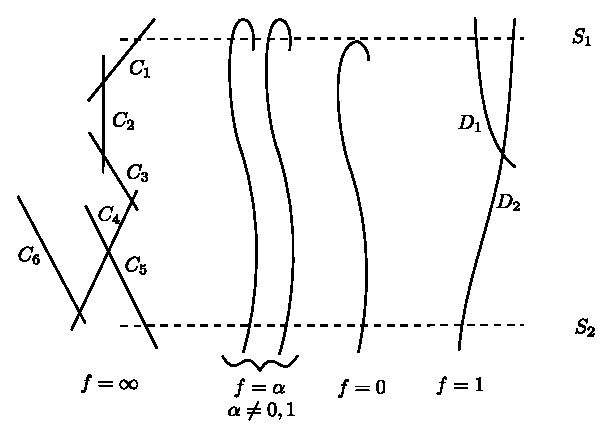
\includegraphics[scale=.8]{figures/chap2-fig2.eps}
\end{figure}
\noindent
where;\pageoriginale\
\begin{enumerate}
\renewcommand{\labelenumi}{\theenumi$^{\circ}$}
\item the dotted line $S_{2}$ is a cross-section of
  $\widetilde{\Lambda}$, and the dotted line $S_{1}$ meets each fiber
  with multiplicity $2$;

\item the singular fiber $f=\infty$ is
  $2C_{1}+4C_{2}+2C_{3}+2C_{4}+C_{5}+C_{6}$ with
  $(C^{2}_{1})=(C^{2}_{4})=(C^{2}_{5})=(C^{2}_{6})=-2$,
  $(C^{2}_{2})=-1$ and $(C^{2}_{3})=-3$;

\item the singular fiber $f=1$ is $D_{1}+D_{2}$, where
  $(D^{2}_{1})=(D^{2}_{2})=-1$, and $D_{1}$ and $D_{2}$ correspond to
  the curves $y=0$ and $x^{2}y+2xy+y+2x=0$, respectively, in the
  decomposition $f-1=y(x^{2}y+2xy+y+2x)$;

\item the fiber $f=0$ is a nonsingular rational curve meeting $S_{1}$
  in a single point with multiplicity $2$;

\item each fiber $f=\alpha(\alpha\in k,\alpha\neq 0,1)$ is a
  nonsingular rational curve meeting $S_{1}$ in two distinct points;

\item $\widetilde{V}$-(the fiber $f=\infty)\cup S_{1}\cup S_{2}\cong
  \mathbb{A}^{2}_{k}$. 
\end{enumerate}
\end{example*}

\subsubsection{}\label{chap2:2.4.5}
Let $f\in k[x,y]$ be an irreducible element such that:
\begin{enumerate}
\renewcommand{\labelenumi}{(\theenumi)}
\item $f$ is a field generator;

\item every irreducible curve of the form $C_{\alpha}:f=\alpha$ with
  $\alpha\in k$ is a nonsingular rational curve with exactly two
  places at infinity.
\end{enumerate}

Even with these conditions satisfied, there might exist a curve
$C_{\alpha}:f=\alpha(\alpha\in k)$ which is not connected, as is shown
by the next:

\begin{example*}
Let $f=y(xy+1)+1$. Then $f$ is an irreducible element. If
$\rho:\widetilde{V}\to \mathbb{P}^{2}_{k}$ is the shortest succession
of quadratic transformations such that the proper transform
$\widetilde{\Lambda}$ of $\Lambda(f)$ has no base points, then
$\widetilde{\Lambda}$ is a pencil of rational curves with two singular
fibers\pageoriginale\ and $\widetilde{\Lambda}$ has the following
configuration:
\begin{figure}[H]
\centering
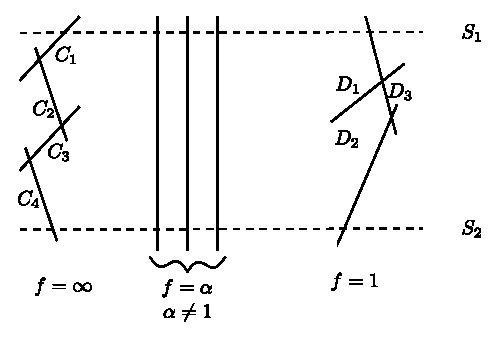
\includegraphics[scale=.9]{figures/chap2-fig3.eps}
\end{figure}
where;
\begin{enumerate}
\renewcommand{\labelenumi}{\theenumi$^{\circ}$}
\item two dotted lines $S_{1}$ and $S_{2}$ are cross-sections of
  $\widetilde{\Lambda}$' 

\item the singular fiber $f=\infty$ is $C_{1}+3C_{2}+2C_{3}+C_{4}$
  with $(C^{2}_{1})=-3$, $(C^{2}_{2})=-1$ and
  $(C^{2}_{3})=(C^{2}_{4})=-2$;

\item the singular fiber $f=1$ is $D_{1}+D_{2}+D_{3}$ with
  $(D^{2}_{1})=(D^{2}_{2})=-1$ and $(D^{2}_{3})=-2$, where $D_{1}$ and
  $D_{2}$ correspond to the curves $y=0$ and $xy+1=0$, respectively,
  in the decomposition $f-1=y(xy+1)$;

\item the fibers $f=\alpha(\alpha\neq 1,\infty)$ are nonsingular
  rational curves;

\item $\widetilde{V}$-(the fiber $f=\infty)\cup S_{1}\cup S_{2}\cup
  D_{3}\cong \mathbb{A}^{2}_{k}$.
\end{enumerate}
\end{example*}

\subsubsection{}\label{chap2:2.4.6}
In the section 6 below we shall show the following result:

Assume that the characteristic of $k$ is zero. Let $f$ be an
irreducible element of $k[x,y]$, and let $C_{\alpha}$ be the curve
defined by $f=\alpha$ for $\alpha\in k$. Then $f=x^{d}y^{e}-1$ for
positive integers $d$ and $e$ such that $(d,e)=1$, after a suitable
change of coordinates $x$\pageoriginale\ and $y$, if the following
conditions are satisfied:
\begin{enumerate}
\renewcommand{\labelenumi}{\theenumi$^{\circ}$}
\item $f$ is a field generator;

\item $C_{\alpha}$ has exactly two places at infinity for almost all
  $\alpha\in k$;

\item $C_{\alpha}$ is connected for every $\alpha\in k$.
\end{enumerate}

\section{Automorphism theorem}\label{chap2:sec3}\pageoriginale\

\subsection{}\label{chap2:3.1}
We shall begin with 

\begin{lemma*}[\cf Nagata {[43; p.\@ 21]} ]
Let $k$ be an algebraically closed field of characteristic $p$. Let
$C_{0}$ be a closed irreducible curve on the affine plane
$\mathbb{A}^{2}_{k}:=\Spec(k[x,y])$ such that $C_{0}$ is defined by
$f=0$ with $f\in k[x,y]$ and that $C_{0}$ is isomorphic to the affine
line $\mathbb{A}^{1}_{k}$. Fix an open immersion of
$\mathbb{A}^{2}_{k}$ into the projective plane $P^{2}_{k}$, and let
$\ell_{0}:=\mathbb{P}^{2}_{k}-\mathbb{A}^{2}_{k}$. Let $C$ be the
closure of $C_{0}$ on $\mathbb{P}^{2}_{k}$, let $P_{0}=C\cap
\ell_{0}$, let $d_{0}=(C\cdot\ell_{0})$ and let $d_{1}$ be the
multiplicity of $C$ at $P_{0}$. Assume that $f$ is a field generator
{\em (\cf \ref{chap2:2.4.1})}. Then $d_{0}$ and $d_{1}$ are divisible by
$d_{0}-d_{1}$. If either $d_{0}$ or $d_{1}$ is not divisible by $p$
then $f$ is a field generator, and $d_{0}$ and $d_{1}$ are divisible
by $d_{0}-d_{1}$.
\end{lemma*}

\begin{proof}
Our proof consists of three steps.
\begin{enumerate}
\renewcommand{\theenumi}{\Roman{enumi}}
\renewcommand{\labelenumi}{\rm(\theenumi)}
\item We may assume with no loss of generality that $d_{0}>d_{1}$. Let
  $\Lambda_{0}$ be an irreducible linear pencil on
  $\mathbb{P}^{2}_{k}$ spanned by $C$ and $d_{0}\ell_{0}$, and let
  $\rho:\widetilde{V}\to P^{2}_{k}$ be the (shortest) succession of
  quadratic transformations such that the proper transform
  $\widetilde{\Lambda}$ of $\Lambda_{0}$ has no base points. By
  assumption and by virtue of \ref{chap2:1.2.2} and \ref{chap2:1.12} when either
  $d_{0}$ or $d_{1}$ is not divisible by $p$, the pencil
  $\widetilde{\Lambda}$ satisfies the properties (1) and (2) of
  \ref{chap2:2.1}; furthermore, the member of $\widetilde{\Lambda}$
  corresponding to $d_{0}\ell_{0}$ of $\Lambda_{0}$ is a reducible
  fiber of $\widetilde{\Lambda}$.

\item As in \ref{chap2:1.3}, find integers $d_{2},\ldots,d_{\alpha}$ and
  $q_{1},\ldots,q_{\alpha}$ by the Euclidean algorithm with respect to
  $d_{0}$ and $d_{1}$. To obtain the\pageoriginale\ morphism $\rho$ we
  have to start with the Euclidean transformation $\sigma:V\to
  \mathbb{P}^{2}_{k}$ associated with an admissible datum
  $\{\mathbb{P}^{2}_{k},\mathbb{A}^{2}_{k},
  C,\ell_{0},\phi,d_{0},d_{1},1\}$. Let $\Lambda$ be the proper
  transform of $\Lambda_{0}$ by $\sigma$ and let $F$ be the member of
  $\Lambda$ corresponding to the member $d_{0}\ell_{0}$ of
  $\Lambda_{0}$. Then $F$ has the weighted graph as given in
  \ref{chap2:1.3}, Figure 1, and $\Lambda$ has a unique base point lying on
  the curve $E(\alpha,q_{\alpha})$ but not on other curves of the
  weighted graph. We shall now apply Lemma \ref{chap2:2.3} to the present
  $V$, $\Lambda$ and $F$.

\item {\bf Case 1.} $\alpha=1$, \iec $d_{0}=q_{1}d_{1}$ with
  $q_{1}\geqq 2$. Then the weighted graph of $F$ is:
\begin{figure}[H]
\centering
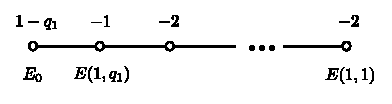
\includegraphics{figures/chap2-fig4.eps} \ .
\end{figure}

\noindent
Now, by virtue of Lemma \ref{chap2:2.3}, we know that
$(E^{2}_{0})=1-q_{1}=-1$, \iec $q_{1}=2$. Then $d_{0}-d_{1}=d_{1}$;
hence $d_{0}-d_{1}$ divides $d_{0}$ and $d_{1}$.

{\bf Case 2.}~$\alpha=2$, \iec $d_{0}=q_{1}d_{1}+d_{2}$ and
$d_{1}=q_{2}d_{2}$ with $q_{2}\geqq 2$. Then the weighted graph of $F$
is:
\begin{figure}[H]
\centering
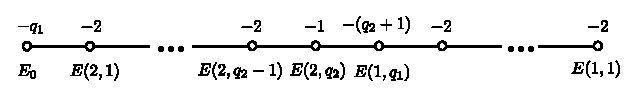
\includegraphics{figures/chap2-fig5.eps} \ .
\end{figure}

Again by Lemma \ref{chap2:2.3} we conclude that $q_{1}=1$. Hence
$d_{0}-d_{1}=d_{2}$. Then $d_{2}$ divides $d_{0}$ and $d_{1}$.

{\bf Case 3.}~$\alpha\geqq 3$. By Lemma \ref{chap2:2.3} we know that
$(E^{2}_{0})=-q_{1}=-1$. Then we can contract the curves $E_{0}$,
$E(2,1),\ldots,E(2,q_{2}-1)$ in this order; in each step of the
contractions we obtain a nonsingular projective surface $V'$, a linear
pencil $\Lambda'$ and a singular fiber $F'$ of\pageoriginale\
$\Lambda'$ to which Lemma \ref{chap2:2.3} can be applied. However, after
contracting the curve $E(2,q_{2}-1)$, the proper transform $E$ of
$E(2,q_{2})$ has self-intersection number $(E^{2})=-q_{3}$ if
$\alpha=3$ and $(E^{2})=-(q_{3}+1)$ if $\alpha\geqq 4$. Note that
$q_{3}\geqq 2$ if $\alpha=3$ and $q_{3}\geqq 1$ if $\alpha\geqq
4$. Hence $(E^{2})\leqq -2$ if $\alpha\geqq 3$. This is a
contradiction. Consequently, we know that $\alpha\leqq 2$ and we are
done.
\end{enumerate}
\end{proof}

\subsection{}\label{chap2:3.2}
\begin{coro*}[(Abhyankar-Moh \cite{2}) ]
  Let $k$ be a field of characteristic $p$. Let $\varphi$ and $\psi$ be
  nonconstant polynomials of degree $m$ and $n$ in $t$ with coefficients
  in $k$. Let $\rho:\mathbb{A}^{1}_{k}=\Spec(k[t])\to
  \mathbb{A}^{2}_{k}=\Spec(k[x,y])$ be a morphism defined by
  $\rho^{\ast}(x)=\varphi(t)$ and $\rho^{\ast}(y)=\psi(t)$, and let
  $f(x,y)$ be an irreducible polynomial in $k[x,y]$ defining the curve
  $\rho(\mathbb{A}^{1}_{k})$. Assume that $k[t]=k[\varphi,\psi]$ and
  that $f$ is a field generator. Then either $m$ divides $n$ or $n$
  divides $m$. If $\text{G.C.D}(m,n)$ is not divisible by $p$ then $f$
  is a field generator, and either $m$ divides $n$ or $n$ divides $m$.
\end{coro*}

\begin{proof}
We may assume that $k$ is algebraically closed, by substituting an
algebraic closure of $k$ for $k$. We may also assume that $m>n$. Fix a
homogeneous coordinate $(X,Y,Z)$ on $\mathbb{P}^{2}_{k}$, and let
$\ell_{0}$ be the line $Z=0$. Let
$\mathbb{A}^{2}_{k}:=\mathbb{P}^{2}_{k}-\ell_{0}$, and let $x:=X/Z$
and $y:=Y/Z$. Then a mapping $t\mapsto (x=\varphi,y=\psi)$ maps
isomorphically $\mathbb{A}^{1}_{k}$ to a curve $C_{0}$ on
$\mathbb{A}^{2}_{k}$. Let $C$ be the closure of $C_{0}$ on
$\mathbb{P}^{2}_{k}$ and let $P_{0}:=C\cap \ell_{0}$. Now write:
\begin{align*}
\varphi(t) &:= a_{m}t^{m}+\cdots+a_{0}\\
\psi(t) &:=b_{n}t^{n}\cdots+b_{0}
\end{align*}
with $a_{m}b_{n}\neq 0$. Then the point $P_{0}$ is $(a_{m},0,0)$, and
the curve $C$ is\pageoriginale\ \break expressed locally at $P_{0}$ in the
following way:
\begin{align*}
X &= a_{m}+a_{m-1}\tau+\cdots+a_{0}\tau^{m}\\
Y &= \tau^{m-n}(b_{n}+b_{n-1}\tau+\cdots+b_{0}\tau^{n})\\
Z &= \tau^{m}
\end{align*}
where $\tau=t^{-1}$. Then $m=(C\cdot\ell_{0})$, and $m-n$ is the
multiplicity of $C$ at $P_{0}$. By virtue of Lemma \ref{chap2:3.1} we
know that $n$ divides $m$.
\end{proof}

\subsection{}\label{chap2:3.3}
Let $k$ be a field of arbitrary characteristic $p$, and let $k[x,y]$
be a polynomial ring in two variables $x$ and $y$ over $k$. We denote
by $\Aut_{k}k[x,y]$ the group of $k$-automorphisms of $k[x,y]$. A
$k$-automorphism $\xi$ ($\sigma$ or $\tau$, \resp) of $k[x,y]$ is
called a {\em linear} ({\em affine} or {\em de Jonqui\`ere}, \resp)
transformation if $\xi$ ($\sigma$ or $\tau$, \resp) has the following
expression: 
\begin{quote}
$\xi(x)=\alpha x+\beta y$, $\xi(y)=\alpha'x+\beta'y$ with $\alpha$,
  $\beta$, $\alpha'$, $\beta'\in k$ such that $\alpha\beta'\neq
  \alpha'\beta$;

$\sigma(x)=\alpha x+\beta y+\gamma$,
  $\sigma(y)=\alpha'x+\beta'y+\gamma'$ with $\alpha$, $\beta$,
  $\gamma$, $\alpha'$, $\beta'$, $\gamma'\in k$ such that
  $\alpha\beta'\neq \alpha'\beta$;

$\tau(x)=\alpha x+f(y)$, $\tau(y)=\beta y+\gamma$, where $f(y)\in
  k[y]$ and $\alpha$, $\beta$, $\gamma\in k$ with $\alpha\beta\neq 0$.
\end{quote}
We denote by $GL(2,k)$ ($A_{2}$ or $J_{2}$, \resp) the subgroup of all
linear (affine or de Jonqui\`ere, \resp) transformations in
$\Aut_{k}k[x,y]$. A $k$-automorphism $\rho$ of $k[x,y]$ is called {\em
  tame} if $\rho$ is an element of the subgroup generated by $A_{2}$
and $J_{2}$. An easy consequence of Corollary \ref{chap2:3.2} is the
following:

\subsubsection{}\label{chap2:3.3.1} 
\noindent \textbf{AUTOMORPHISM THEOREM (\cf Nagata \cite{43};
    Abhyankar-Moh \cite{2} and many others).}
  Let\pageoriginale\ $k$ be a field of arbitrary characteristic. Then every
  $k$-automorphism of $k[x,y]$ is tame.


\begin{proof}
Let $\rho$ be a $k$-automorphism of $k[x,y]$ and let 
\begin{align*}
\rho(x) &:= f(x,y)=f_{0}(x,y)+f_{1}(x,y)+\cdots+f_{m}(x,y)\\
\rho(y) &:= g(x,y)=g_{0}(x,y)+g_{1}(x,y)+\cdots+g_{n}(x,y)
\end{align*}
where $f_{i}(x,y)$ and $g_{j}(x,y)$ are the $i$-th and the $j$-th
homogeneous parts of $f$ and $g$, respectively, for $0\leqq i\leqq m$
and $0\leqq j\leqq n$, and where $f_{m}(x,y)\neq 0$ and
$g_{n}(x,y)\neq 0$. After a suitable change of coordinates $x$ and $y$
by a linear transformation we may assume that $f_{m}(x,0)\neq 0$ and
$g_{n}(x,0)\neq 0$. Let $\varphi(x):=f(x,0)$ and
$\psi(x):=g(x,0)$. Then $k[x]=k[\varphi,\psi]$. Let
$\tau:\mathbb{A}^{1}_{k}=\Spec(k[x])\to
\mathbb{A}^{2}_{k}=\Spec(k[x',y'])$ be a morphism defined by
$\tau^{\ast}(x')=\varphi(x)$ and $\tau^{\ast}(y')=\psi(x)$, let
$C_{0}=\tau(\mathbb{A}^{1}_{k})$, and let $f'(x',y')$ be an
irreducible element in $k[x',y']$ defining $C_{0}$. Then $f'$ is a
field generator; this is clear because $\rho$ is an automorphism of
$k[x,y]$. By Corollary \ref{chap2:3.2} we conclude that either $m|n$ or
$n|m$. Besides, it is easily ascertained that if $mn>1$ then
$f_{m}(x,y)=\alpha\lambda^{m}$ and $g_{n}(x,y)=\beta\lambda^{n}$ for a
common linear factor $\lambda$ in $x$ and $y$ and for $\alpha$,
$\beta\in k^{\ast}$\footnote{Since the curve $f(x,y)=0$ is isomorphic
  to $\mathbb{A}^{1}_{k}$, we know that $f_{m}(x,y)=\lambda^{m}_{1}$
  for a linear factor $\lambda_{1}$; similarly,
  $g_{n}(x,y)=\lambda^{n}_{2}$. Since the curves $f(x,y)=0$ and
$g(x,y)=0$ intersect in a single point transversely on
$\mathbb{A}^{2}_{k}=\Spec(k[x,y])$, we know by Bezout's Theorem that
$\lambda_{2}=\gamma\lambda_{1}$ with $\gamma\in k^{\ast}$ unless
  $mn=1$.}. Assuming that $m=nd>1$, define a $k$-automorphism $\sigma$
of $k[x,y]$ by\pageoriginale\ $\sigma(x)=x-\gamma y^{d}$ and
$\sigma(y)=y$, where $\alpha=\gamma\beta^{d}$. Then $\sigma\rho(x)$
has degree smaller than $m$. Thus, we can finish our proof by
induction on $\max(m,n)$.
\end{proof}

\subsubsection{}\label{chap2:3.3.2}
More precisely, we know the following structure theorem on\break 
$\Aut_{k}k[x,y]$:

\begin{lemma*}[(\cf Nagata [43; Th.\@ 3.3]; Kambayashi \cite{25}) ]
  $\Aut_{k}k[x,y]$ is an amalgamated product of $A_{2}$ and
  $J_{2}$. Namely, if $\sigma_{i}\in A_{2}-J_{2}$ 
  \setcounter{pageoriginal}{130}
  $(1\leqq i\leqq r-1)$,\pageoriginale\ $\tau_{j}\in J_{2}-A_{2}(1\leqq
  j\leqq r)$, then
  $\tau_{1}\sigma_{1}\tau_{2}\sigma_{2}\ldots\tau_{r-1}\sigma_{r-1}\tau_{r}\not\in
  A_{2}$. 
\end{lemma*}

For the convenience of readers, we shall give a (sketchy) proof in the
next paragraph.

\subsection{}\label{chap2:3.4}
Let $\tau:\tau(x)=\alpha x+f(y)$ and $\tau(y)=\beta y+\gamma$ be a de
Jonqui\`ere transformation of $k[x,y]$. $\tau$ defines a birational
automorphism $T$ of $\mathbb{P}^{2}_{k}$ by setting:
$T^{\ast}(X)=\alpha XZ^{n-1}+F(Y,Z)$, $T^{\ast}(Y)=\beta
YZ^{n-1}+\gamma Z^{n}$ and $T^{\ast}(Z)=Z^{n}$, where $x=X/Z$,
$y=Y/Z$, $n:=\deg_{y}f(y)$ and $F(Y,Z):=Z^{n}f(Y/Z)$.\footnote{If
  $n=\deg_{y}f(y)$, $\tau$ is called a de Jonqui\`ere transformation
  of degree $n$.} We assume that $n>1$. Then it is easy to see that
$P_{0}:(X,Y,Z)=(1,0,0)$ is a unique fundamental point of $T$ on
$\mathbb{P}^{2}_{k}$ and the line $\ell_{0}:Z=0$ is a unique
fundamental curve of $T$ on $\mathbb{P}^{2}_{k}$. Let $\varphi_{1}$ be
a quadratic transformation with center at $P_{0}$. Now eliminating
fundamental points (including infinitely near fundamental points) of
$T$ by the (shortest) succession of quadratic transformations, which
start with $\varphi_{1}$, we have a nonsingular projective surface $V$
and birational morphisms $\varphi$, $\psi:V\to \mathbb{P}^{2}_{k}$
such that $T=\psi\cdot\varphi^{-1}$.

\subsubsection{}\label{chap2:3.4.1}
\begin{lemma*}
  With the above notations we have:
  \begin{enumerate}
    \renewcommand{\labelenumi}{\rm(\theenumi)}
  \item $\varphi^{-1}(\ell_{0})$ has the following weighted graph:
    \begin{figure}[H]
      \centering
      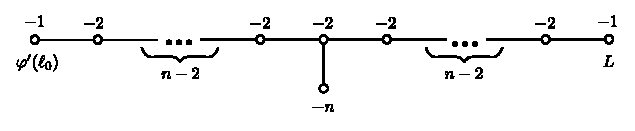
\includegraphics{figures/chap2-fig6.eps}
    \end{figure}
    where\pageoriginale\ each vertex stands for a nonsingular rational
    curve; the vertex with weight $-n$ corresponds to the proper transform
    of $\varphi^{-1}(P_{0})$ by $\varphi\varphi^{-1}_{1}$.
    
  \item Let $L$ be the curve with weight $-1$ other than
    $\varphi'(\ell_{0})$. Then $\psi(L)$ is the line at infinity of a
    new projective plane $\mathbb{P}^{2}_{k}$.
    
  \item The point $Q:=(1,0,0)$ on the new projective plane
    $\mathbb{P}^{2}_{k}$ is a unique fundamental point of $T^{-1}$.
  \end{enumerate}
\end{lemma*}

\begin{proof}
Straightforward computation. See also Russell [48; 4.2].
\end{proof}

\subsubsection{}\label{chap2:3.4.2}
Note that if $\sigma:\sigma(x)=\alpha x+\beta y+\gamma$ and
$\sigma(y)=\alpha'x+\beta'y+\gamma'$ is an affine transformation not
in $J_{2}$, \iec $\alpha'\neq 0$ then the associated biregular
automorphism $\Sigma:(X,Y,Z)\mapsto (\alpha X+\beta Y+\gamma
Z,\alpha'X+\beta'Y+\gamma'Z,Z)$ of $\mathbb{P}^{2}_{k}$ maps the point
$(1,0,0)$ to $(\alpha,\alpha',0)$ which is distinct from
$(1,0,0)$. With this remark in mind we can easily show:

\begin{lemma*}
Let $\sigma_{i}\in A_{2}-J_{2}(1\leqq i\leqq r-1)$, let $\tau_{j}\in
J_{2}-A_{2}(1\leqq j\leqq r)$ and let
$\rho:\tau_{1}\sigma_{1}\ldots\tau_{r-1}\sigma_{r-1}\tau_{r}$. Let
$n_{j}$ be the degree of $\tau_{j}$ for $1\leqq j\leqq r$. Let
$\Sigma_{i}(1\leqq i\leqq r-1)$, $T_{j}(1\leqq j\leqq r)$ and $R$ be
birational automorphisms of $\mathbb{P}^{2}_{k}$ associated with
$\sigma_{i}$, $\tau_{j}$ and $\rho$, respectively. Then, by
elimination of indeterminacy of a birational automorphism $\rho$, we
obtain a nonsingular projective surface $W$ and birational morphisms
$\phi$, $\psi:W\to \mathbb{P}^{2}_{k}$ such that:
\begin{enumerate}
\renewcommand{\labelenumi}{\rm(\theenumi)}
\item $R=\psi\cdot\phi^{-1}$, where
  $R:=T_{r}\Sigma_{r-1}T_{r-1}\ldots\Sigma_{1}T_{1}$; 

\item $\phi^{-1}(\ell_{0})$ has the following weighted graph:
\begin{figure}[H]
\centering
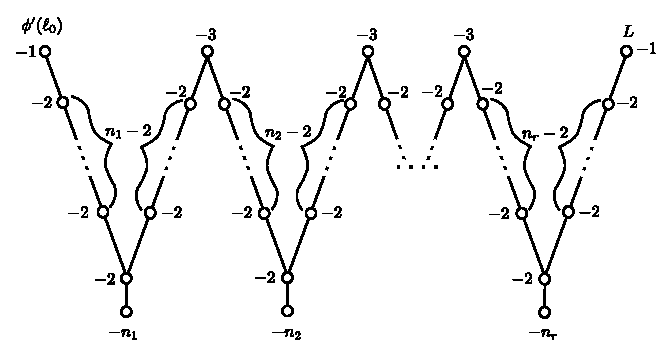
\includegraphics[scale=.95]{figures/chap2-add-fig2.eps}
\end{figure}
where,\pageoriginale\ if $L$ is the curve corresponding to the vertex
with weight $-1$ other than $\phi'(\ell_{0})$, then $\psi(L)$ is the
line at infinity of a new projective plane $\mathbb{P}^{2}_{k}$;

\item $n_{j}>1$ for $1\leqq j\leqq r$.
\end{enumerate}
\end{lemma*}

\subsubsection{}\label{chap2:3.4.3}
By virtue of Lemma \ref{chap2:3.4.2}, it is clear that $\rho\not\in
A_{2}$; if $\rho\in A_{2}$ then $\ell_{0}$ would not be a fundamental
curve. Therefore we completed a proof of Lemma \ref{chap2:3.3.2}.

\subsection{}\label{chap2:3.5}
We shall prove in this paragraph the following:

\begin{theorem*}[Igarashi-Miyanishi \cite{24} ]
Let $k$ be a field of characteristic zero.\footnote{The theorem holds
  for an arbitrary characteristic $p$ if $(n,p)=1$. Indeed, Lemmas
  \ref{chap2:3.5.1} and \ref{chap2:3.5.2} hold true with this condition,
  while Lemmas \ref{chap2:3.5.3} and \ref{chap2:3.5.4} hold true without any
restriction.} Let $F$ be a
finite subgroup of order $n$ of $\Aut_{k}k[x,y]$. Then there exists an
element $\rho$ of $\Aut_{k}k[x,y]$ such that $\rho^{-1}F\rho$ is
contained in $GL(2,k)$.
\end{theorem*}

The proof will be given in the subparagraphs \ref{chap2:3.5.1} $\sim$
\ref{chap2:3.5.5}.

\subsubsection{}\label{chap2:3.5.1}
\begin{lemma*}
  With\pageoriginale\ the notations and assumptions as above, if $F$ is
  contained in $A_{2}$, then $F$ is conjugate to a finite subgroup of $GL(2,k)$.
\end{lemma*}

\begin{proof}
It suffices to show that $F$ has a fixed point on the affine plane
$\mathbb{A}^{2}_{k}$. Indeed, let $\rho$ be an affine transformation
defined by 
$$
\rho
\begin{pmatrix}
x\\
y\\
1
\end{pmatrix}
=
\begin{pmatrix}
1 & 0 & s\\
0 & 1 & t\\
0 & 0 & 1
\end{pmatrix}
\begin{pmatrix}
x\\
y\\
1
\end{pmatrix}.
$$
Then $\rho^{-1}F\rho\subset GL(2,k)$ if and only if the point
$(x=s, y=t)$ on $\mathbb{A}^{2}_{k}$ is fixed under $F$. Each
$\sigma\in A_{2}$ has a matrix representation:
$$
\sigma
\begin{pmatrix}
x\\
y\\
1
\end{pmatrix}
=
\begin{pmatrix}
\alpha(\sigma) & \beta(\sigma) & a(\sigma)\\
\gamma(\sigma) & \delta(\sigma) & b(\sigma)\\
0 & 0 & 1
\end{pmatrix}
\begin{pmatrix}
x\\
y\\
1
\end{pmatrix}.
$$
Let $\ell(\sigma)={}^{t}(a(\sigma),b(\sigma))$ and let $M(\sigma)$ be
an invertible matrix such that
$$
M(\sigma)=
\begin{pmatrix}
\alpha(\sigma) & \beta(\sigma)\\
\gamma(\sigma) & \delta(\sigma)
\end{pmatrix}.
$$
For $\sigma$, $\tau\in A_{2}$, we have $\ell(\sigma\cdot
\tau)=\ell(\sigma)+M(\sigma)\ell(\tau)$ and
$M(\sigma\cdot\tau)=M(\sigma)\cdot M(\tau)$. Then
$\ell_{0}={}^{t}(s_{0},t_{0})$ is a fixed point of $F$ if and only if
$\ell(\sigma)=\ell_{0}-M(\sigma)\ell_{0}$ for every $\sigma$ of
$F$. Set $\ell_{0}:=\left\{{\displaystyle{\mathop{\sum}_{\tau\in
      F}}}\ell(\tau)\right\}/n$. Since
$$
\frac{1}{n}\sum_{\tau\in F}\ell(\sigma\cdot
\tau)=\ell(\sigma)+M(\sigma)\left(\frac{1}{n}\sum_{\tau\in
  F}\ell(\tau)\right),
$$
we\pageoriginale\ have then
$\ell(\sigma)=\ell_{0}-M(\sigma)\ell_{0}$. Hence $\ell_{0}$ gives rise
to a point $Q$ of $\mathbb{A}^{2}_{k}$ fixed under $F$. 
\end{proof}

\subsubsection{}\label{chap2:3.5.2}
\begin{lemma*}
  With the notations and assumptions as above, if $F\subset J_{2}$, then
  $F$ is conjugate to a finite subgroup of $GL(2,k)$.
\end{lemma*}

\begin{proof}
Each element $\sigma\in J_{2}$ acts on $\mathbb{A}^{2}_{k}$ in the
following way:
$$
\sigma(x)=\alpha(\sigma)x+f_{\sigma}(y)\quad\text{and}\quad
\sigma(y)=\beta(\sigma)y+\gamma(\sigma), 
$$
where $f_{\sigma}(y)\in k[y]$; $\alpha(\sigma)$, $\beta(\sigma)$,
$\gamma(\sigma)\in k$; $\alpha(\sigma)\cdot \beta(\sigma)\neq 0$. For
$\sigma$, $\tau\in J_{2}$, we have:
$$
\alpha(\sigma\cdot \tau)=\alpha(\sigma)\cdot
\alpha(\tau),\beta(\sigma\cdot \tau)=\beta(\sigma)\cdot
\beta(\tau),\gamma(\sigma\cdot \tau)=\gamma(\tau)+\beta(\tau)\gamma(\sigma)
$$
and
$f_{\sigma\cdot\tau}(y)=f_{\tau}(\beta(\sigma)y+\gamma(\sigma))+\alpha(\tau)f_{\sigma}(y)$.  

Let $J^{0}_{2}$ be the subgroup of $J_{2}$ such that
$\gamma(\sigma)=0$. Let
$\epsilon=\left\{{\displaystyle{\mathop{\sum}_{\tau\in
      F}}}\gamma(\tau)\right\}$ $/n$. Then
$\gamma(\sigma)=\epsilon-\beta(\sigma)\epsilon$ for every $\sigma$ of
$F$. Replacing $y$ by $y-\epsilon$, we may assume that $F$ is
contained in $J^{0}_{2}$. We shall now look for a polynomial $g(y)\in
k[y]$ such that $\sigma(x+g(y))=\alpha(\sigma)(x+g(y))$ for every
$\sigma\in F$. If such a polynomial exists, we have
$\rho^{-1}\sigma\rho(x)=\alpha(\sigma)x$ and
$\rho^{-1}\sigma\rho(y)=\beta(\sigma)y$ for every $\sigma\in F$,
setting $\rho(x)=x+g(y)$ and $\rho(y)=y$. Namely, $F\subset
GL(2,k)$. Now $g(y)$ satisfies $\sigma(x+g(y))=\alpha(\sigma)(x+g(y))$
for every $\sigma\in F$ if and only if
$f_{\sigma}(y)=\alpha(\sigma)g(y)-g(\beta(\sigma)y)$ for every
$\sigma\in F$. Write $f_{\sigma}(y)$ in the form:
$$
f_{\sigma}(y)=\frac{\alpha(\sigma)}{\alpha(\sigma\cdot\tau)}f_{\sigma\cdot
  \tau}(y)-\frac{1}{\alpha(\tau)}f_{\tau}(\beta(\sigma)y). 
$$
Then\pageoriginale\
$nf_{\sigma}(y)=\alpha(\sigma){\displaystyle{\mathop{\sum}_{\tau\in
      F}}}\dfrac{f_{\sigma\cdot
      \tau}(y)}{\alpha(\sigma\cdot\tau)}-{\displaystyle{\mathop{\sum}_{\tau
    \in F}}}\dfrac{f_{\tau}(\beta(\sigma)y)}{\alpha(\tau)}$. Set
  $g(y):=\dfrac{1}{n}{\displaystyle{\mathop{\sum}_{\tau\in
        F}}}\dfrac{f_{\tau}(y)}{\alpha(\tau)}$. Then
  $f_{\sigma}(y)=\alpha(\sigma)g(y)-g(\beta(\sigma)y)$ for every
  $\sigma\in F$. This completes the proof.
\end{proof}

\subsubsection{}\label{chap2:3.5.3}
\begin{lemma*}
  Let $F$ be a finite subgroup of $\Aut_{k}k[x,y]$. Let $\sigma$ be an
  element of $F$. Then there exists an element $\rho$ in
  $\Aut_{k}k[x,y]$ such that $\rho^{-1}\sigma\rho$ is contained in
  either $A_{2}$ or $J_{2}$ and $\rho^{-1}(F\cap (A_{2}\cup
  J_{2}))\rho\subset \rho^{-1}F\rho\cap (A_{2}\cup J_{2})$, where
  $A_{2}\cup J_{2}$ is the set-theoretic union of $A_{2}$ and $J_{2}$ in
  $\Aut_{k}k[x,y]$. 
\end{lemma*}

\begin{proof}
Our proof consists of three steps.
\begin{enumerate}
\renewcommand{\theenumi}{\Roman{enumi}}
\renewcommand{\labelenumi}{(\theenumi)}
\item By virtue of Lemma \ref{chap2:3.3.2} we may write $\sigma$ in one
  of the following ways:
\begin{enumerate}
\renewcommand{\theenumii}{\roman{enumii}}
\renewcommand{\labelenumii}{\rm(\theenumii)$_{r}$}
\item $\sigma=\sigma_{1}\tau_{1}\ldots\tau_{r-1}\sigma_{r}\tau_{r}$,
  where $\sigma_{i}\in A_{2}-A_{2}\cap J_{2}(1\leqq i\leqq r)$,
  $\tau_{j}\in J_{2}-A_{2}\cap J_{2} (1\leqq j\leqq r-1)$ and
  $\tau_{r}\in J_{2}$;

\item
  $\sigma=\tau'_{1}\sigma'_{1}\ldots\sigma'_{r-1}\tau'_{r}\sigma'_{r}$,
  where $\tau'_{i}\in J_{2}-A_{2}\cap J_{2}(1\leqq i\leqq r)$,
  $\sigma'_{j}\in A_{2}-A_{2}\cap J_{2}(1\leqq j\leqq r-1)$ and
  $\sigma'_{r}\in A_{2}$. 
\end{enumerate}
We shall prove the following assertions for every $r\geqq 1$:
\begin{enumerate}
\renewcommand{\theenumii}{\arabic{enumii}}
\renewcommand{\labelenumii}{\rm(\theenumii)$_{r}$}
\item if $\sigma$ is written in the way $({\rm i})_{r}$ then there
  exists an element $\rho$ of $\Aut_{k}k[x,y]$ such that
  $\rho^{-1}\sigma\rho$ is written in the way $({\rm ii})_{r-1}$ and
  $\rho^{-1}(F\cap (A_{2}\cup J_{2}))\rho\subset \rho^{-1}F\rho\cap
  (A_{2}\cup J_{2})$;

\item If $\sigma$ is written in the way $({\rm ii})_{r}$ then there
  exists an element $\rho$ of $\Aut_{k}k[x,y]$ such that
  $\rho^{-1}\sigma\rho$ is written in the way $({\rm i})_{r-1}$ and
  $\rho^{-1}(F\cap (A_{2}\cup J_{2}))\rho\subset \rho^{-1}F\rho\cap
  (A_{2}\cup J_{2})$; where\pageoriginale\ $(1)_{1}$ and $(2)_{1}$ are
  understood, respectively as:
$$
(1)_{1}~\sigma\in A_{2};\quad (2)_{1}~\sigma\in J_{2}.
$$
It is apparent that the assertion in Lemma follows from the above
assertions. 
\end{enumerate}

\item {\em Proof of the assertion $(1)_{r}$}. Since $\sigma^{n}=1$ for
  some integer $n>0$, we have:
$$
\sigma^{n}=\underbrace{(\sigma_{1}\tau_{1}\ldots\sigma_{r}\tau_{r})\ldots(\sigma_{1}\tau_{1}\ldots\sigma_{r}\tau_{r})}_{n\text{-times}}=1.
$$
Since
$(\tau_{1}\ldots\sigma_{r}\tau_{r})(\sigma_{1}\tau_{1}\ldots\sigma_{r}\tau_{r})\ldots(\sigma_{1}\tau_{1}\ldots\sigma_{r}\tau_{r})=\sigma^{-1}_{1}\in
A_{2}$, Lemma \ref{chap2:3.3.2} implies that $\tau_{r}\in A_{2}\cap
J_{2}$; indeed, if $\tau_{r}\not\in A_{2}$ we would have a
contradiction. If $r=1$ then $\sigma=\sigma_{1}\tau_{1}\in A_{2}$,
\iec $(1)_{1}$ holds. If $r>1$, we know again by Lemma \ref{chap2:3.3.2}
that $\sigma_{r}\tau_{r}\sigma_{1}\in A_{2}\cap J_{2}$ because 
\begin{multline*}
  (\tau_{1}\ldots\tau_{r-1}) (\sigma_{r}\tau_{r}\sigma_{1})
  (\tau_{1}\ldots\tau_{r-1})\ldots (\sigma_{r}\tau_{r}\sigma_{1})
  (\tau_{1}\ldots\tau_{r-1})\\ 
  = (\sigma_{r}\tau_{r}\sigma_{1})^{-1}\in A_{2}. 
\end{multline*}
Let $h=\sigma_{r}\tau_{r}\sigma_{1}$. Then
$\sigma_{r}\tau_{r}=h\sigma^{-1}_{1}$, and
$\sigma^{-1}_{1}\sigma\sigma_{1}=\tau_{1} \sigma_{2} \ldots
\sigma_{r-1}$ $\tau_{r-1}h$. Thus
$\sigma^{-1}_{1}\sigma\sigma_{1}$ has an expression as in $({\rm
  ii})_{r-1}$. We shall show that $\sigma^{-1}_{1}(F\cap (A_{2}\cup
J_{2}))\sigma_{1}\subset \sigma^{-1}_{1}F\sigma_{1}\cap (A_{2}\cup
J_{2})$. Let $\sigma_{0}$ be an element of $F\cap (A_{2}\cup
J_{2})$. Since $\sigma\cdot \sigma_{0}\in F$ and $(\sigma\cdot
\sigma_{0})^{m}=1$ for some integer $m>0$, we have:
$$
(\sigma\cdot
\sigma_{0})^{m}=\underbrace{(\sigma_{1}\tau_{1}\ldots\sigma_{r}\tau_{r}\sigma_{0})\ldots(\sigma_{1}\tau_{1}\ldots\sigma_{r}\tau_{r}\sigma_{0})}_{m\text{-times}}=1. 
$$
Since
$(\tau_{1}\sigma_{2}\ldots\sigma_{r}\tau_{r}\sigma_{0})(\sigma_{1}\tau_{1}\ldots\sigma_{r}\tau_{r}\sigma_{0})\ldots(\sigma_{1}\tau_{1}\ldots\sigma_{r}\tau_{r}\sigma_{0})=\sigma^{-1}_{1}\in
A_{2}$ and\pageoriginale\ since $\sigma_{r}\tau_{r}\in A_{2}-A_{2}\cap
J_{2}$, Lemma \ref{chap2:3.3.2} implies that $\sigma_{0}\not\in
J_{2}-A_{2}\cap J_{2}$, \iec $\sigma_{0}\in A_{2}$. Since this is true
for every element $\sigma_{0}$ of $F\cap (A_{2}\cup J_{2})$ we know
that $F\cap (A_{2}\cup J_{2})=F\cap A_{2}$. Then
$\sigma^{-1}_{1}(F\cap A_{2})\sigma_{1}\subset
\sigma^{-1}_{1}F\sigma_{1}\cap (A_{2}\cup J_{2})$ because
$\sigma_{1}\in A_{2}$. Thus we have only to take $\sigma_{1}$ as
$\rho$.

\item {\em Proof of the assertion $(2)_{r}$.} A proof will be only
  sketchy because it is similar to the proof of $(1)_{r}$. Since
  $\sigma^{n}=1$ for some integer $n>0$ we conclude by Lemma
  \ref{chap2:3.3.2} that $\sigma'_{r}\in A_{2}\cap J_{2}$. If $r=1$ then
  $\sigma=\tau'_{1}\sigma'_{1}\in J_{2}$, \iec $(2)_{1}$ holds. If
  $r>1$, Lemma \ref{chap2:3.3.2} again implies that
  $\tau'_{r}\sigma'_{r}\tau'_{1}\in A_{2}\cap J_{2}$. Let
  $h'=\tau'_{r}\sigma'_{r}\tau'_{1}$. Then
  $\tau'_{r}\sigma'_{r}=h'{\tau'}^{-1}_{1}$ and
  ${\tau'}^{-1}_{1}\sigma
  \tau'_{1}=\sigma'_{1}\tau'_{2}\ldots\tau'_{r-1}\sigma'_{r-1}h'$. Thus
  ${\tau'}^{-1}_{1}\sigma\tau'_{1}$ has an expression as in $({\rm
    i})_{r-1}$. We shall show that ${\tau'}^{-1}_{1}(F\cap (A_{2}\cup
  J_{2}))\tau'_{1}\subset{\tau'}^{-1}_{1}F\tau'_{1}\cap (A_{2}\cup
  J_{2})$. Let $\sigma_{0}$ be an arbitrary element of $F\cap
  (A_{2}\cup J_{2})$. Since $\sigma\cdot\sigma_{0}\in F$ and
  $(\sigma\cdot\sigma_{0})^{m}=1$ for some integer $m>0$, a similar
  argument as in step (II) shows that $\sigma_{0}\in J_{2}$. Hence
  $F\cap (A_{2}\cup J_{2})=F\cap J_{2}$. Then
  ${\tau'}^{-1}_{1}(FJ_{2})\tau'_{1}\subset
  {\tau'}^{-1}_{1}F\tau'_{1}\cap (A_{2}\cup J_{2})$ because
  $\tau'_{1}\in J_{2}$. Thus we have only to take $\tau'_{1}$ as
  $\rho$.
\end{enumerate}
\end{proof}

\subsubsection{}\label{chap2:3.5.4}
\begin{lemma*}
  Let $F$ be a finite subgroup of $\Aut_{k}k[x,y]$. Then there exists an
  element $\rho$ in $\Aut_{k}k[x,y]$ such that $\rho^{-1}F\rho$ is
  contained in either $A_{2}$ or $J_{2}$.
\end{lemma*}

\begin{proof}
Lemma \ref{chap2:3.5.3} tells us the following: If $F$ has an element
$\sigma$ not in $A_{2}$ and $J_{2}$ then there exists an element
$\rho$ of $\Aut_{k}k[x,y]$ such that $|\rho^{-1}F\rho\cap(A_{2}\cup
J_{2})|>|F\cap (A_{2}\cup J_{2})|$. Hence, by substituting a suitable
conjugate of $F$ for $F$, we may assume that $F\subset A_{2}\cup
J_{2}$. If $F$ is not contained in $A_{2}$ or $J_{2}$, then there\pageoriginale\
exist two elements $\alpha$ and $\beta$ in $F$ such that $\alpha\in
A_{2}-A_{2}\cap J_{2}$ and $\beta\in J_{2}-(A_{2}\cap J_{2})$. Then
Lemma \ref{chap2:3.3.2} implies that $\alpha\cdot \beta$ is not of finite
order. This contradicts the fact that $\alpha\cdot \beta\in F$. Hence
either $F\subset A_{2}$ or $F\subset J_{2}$.
\end{proof}

\subsubsection{}\label{chap2:3.5.5}
\begin{lemma*}
  \ref{chap2:3.5.4} combined with Lemmas \ref{chap2:3.5.1} and \ref{chap2:3.5.2}
  completes a proof of Theorem \ref{chap2:3.5}.
\end{lemma*}

\subsection{}\label{chap2:3.6}
In the present and the next paragraphs we shall apply Theorem
\ref{chap2:3.5}, in order to obtain two partial answers of the following:

\begin{conjecture*}
Let $k$ be an algebraically closed field, and let $A$ be a regular
$k$-subalgebra of a polynomial ring $k[x,y]$ such that $k[x,y]$ is a
flat $A$-module of finite type. Then $A$ is a polynomial ring over $k$.
\end{conjecture*}

The first result is stated as follows:

\begin{prop*}
Let $k$ be an algebraically closed field of characteristic zero. Let
$X$ be a nonsingular affine surface and let $f:\mathbb{A}^{2}_{k}\to
X$ be an \'etale finite surjective morphism. Then $f$ is an isomorphism.
\end{prop*}

This result will be proved in the subparagraphs \ref{chap2:3.6.1} $\sim$
\ref{chap2:3.6.4}. 

\subsubsection{}\label{chap2:3.6.1}
\begin{defi*}
  Let $X$ and $Z$ be nonsingular varieties defined over $k$ and let
  $h:Z\to X$ be an \'etale finite morphism. A pair $(Z,h)$ is called
  {\em a Galois covering of $X$ with group} $F$ if there exist a finite
  group $F$ acting freely on $Z$ and a $k$-isomorphism
  $\varphi:Z/F\xrightarrow{\sim}X$\pageoriginale\ between the quotient
  variety $Z/F$ and $X$ such that $h=\varphi q$, where $q:Z\to Z/F$ is
  the canonical quotient morphism.
\end{defi*}

\subsubsection{}\label{chap2:3.6.2}
\begin{lemma*}
  Let $f:X\to Y$ be an \'etale finite morphism of a nonsingular variety
  $X$ onto a nonsingular variety $Y$. Then there exist an \'etale finite
  morphism $h:Z\to X$ of a nonsingular variety $Z$ onto $X$, a finite
  group $G$ and a subgroup $H$ of $G$ such that:
  \begin{enumerate}
    \renewcommand{\labelenumi}{\rm(\theenumi)}
  \item $g:f\cdot h:Z\to Y$ is a Galois covering with group $G$;
    
  \item $h:Z\to X$ is a Galois covering with group $H$.
  \end{enumerate}
\end{lemma*}

\begin{proof}
Let $n:=[k(X):k(y)]$ and let
$\widetilde{S}:=\fprod{\fprod{\fprod{X}{X}{Y}}{\ldots}{Y}}{X}{Y}$ be
the $n$-th iterated fiber product of $X$ over $Y$. Let $F$ be the
closed subset of $\widetilde{S}$ consisting of all $n$-tuples
$(x_{1},\ldots,x_{n})$ in which two or more of $x_{i}$'s coincide with
each other. Let $Z:=\widetilde{S}-F$, and let $S_{n}$ be the symmetric
group on $n$ letters. Then $S_{n}$ acts freely on $Z$. Let $h:Z\to X$
be the projection onto the first factor, and let $S_{n-1}$ be the
symmetric group on $n-1$ letters, which we let act on $Z$ in such a
way that
$$
\sigma(x_{1},\ldots,x_{n})=(x_{1},\sigma(x_{2},\ldots,x_{n}))\quad\text{for}\quad
\sigma\in S_{n-1}. 
$$
Then $S_{n-1}\subset S_{n}$. Since $h^{-1}(x)$ consists of $(n-1)!$
points for every $x\in X$, $h$ is an \'etale finite morphism. Thus
$q:=f\cdot h:Z\to Y$ is also an \'etale finite morphism. It is obvious
that $Y\cong Z/S_{n}$ with the quotient morphism $q:Z\to Y$ and
$X\cong Z/S_{n-1}$ with the quotient morphism $h:Z\to X$. We have now
only to set $G:=S_{n}$ and $H:=S_{n-1}$.
\end{proof}

\subsubsection{}\label{chap2:3.6.3}
\begin{lemma*}
  With\pageoriginale\ the notations of \ref{chap2:3.6.2}, if $X$ is simply
  connected, \iec 
  $X$ has no nontrivial \'etale finite coverings, then $f:X\to Y$ is a
  Galois covering.
\end{lemma*}

\begin{proof}
Since $X$ is simply connected, $h:Z\to X$ splits. Namely there exists
a regular cross-section $s:X\to Z$ such that the morphism $H\times
X\to Z$ defined by $(h,x)\mapsto hs(x)$ is an isomorphism. Therefore
the number of connected components of $Z$, which are all isomorphic to
$X$, is the order $|H|$ of $H$. Let $X_{0}:=s(X)$ and let $F$ be the
subgroup of $G$ consisting of all elements $g$ of $G$ such that
$g(X_{0})=X_{0}$. If $X_{1}$ is a connected component of $Z$ distinct
from $X_{0}$ and if $g$ is an element of $G$ such that
$g(X_{0})=X_{1}$, then $g_{1}F$ is the set of all elements of $G$
which send $X_{0}$ to $X_{1}$. Hence $Z\cong X\times G/F$, and
$|G/F|=|H|$. Therefore the morphism $q|_{X_{0}}:X_{0}\to Y$ has degree
$|G|/|H|=|F|$. Since $F$ acts freely on $X_{0}$, we know that a pair
$(X_{0},g|_{X_{0}})$ is a Galois covering of $Y$ with group
$F$. Finally, since $X\cong X_{0}$, $f:X\to Y$ is a Galois covering
with group $F$.
\end{proof}

\subsubsection{}\label{chap2:3.6.4}
\begin{proofofprop*}[3.6 ]
  Since $\mathbb{A}^{2}_{k}$ is simply connected (if the characteristic
  of $k$ is zero), we know by applying Lemma \ref{chap2:3.6.3} that
  $f:\mathbb{A}^{2}_{k}\to X$ is a Galois covering with group $F$. But
  since every finite subgroup of $\Aut_{k}k[x,y]$ has a fixed point on
  $\mathbb{A}^{2}_{k}$ by virtue of Theorem \ref{chap2:3.5}, we know that
  $F$ can not act freely on $\mathbb{A}^{2}_{k}$. Therefore, $F\cong
  (1)$, and $f$ is an isomorphism. This completes a proof of Proposition
  \ref{chap2:3.6}.
\end{proofofprop*}

\subsection{}\label{chap2:3.7}
Another application of Theorem \ref{chap2:3.5} is the following
proposition which\pageoriginale\ is a slight improvement of Serre's
result (\cf Lemma \ref{chap2:3.7.1} below):

\begin{prop*}
Let $k$ be a field of characteristic zero, and let $F$ be a finite
subgroup of $\Aut_{k}k[x,y]$. Then the following conditions are
equivalent to each other:
\begin{enumerate}
\renewcommand{\labelenumi}{\rm(\theenumi)}
\item $k[x,y]^{F}$ is a regular ring;

\item $k[x,y]^{F}$ is a polynomial ring over $k$;
\end{enumerate}
where $k[x,y]^{F}$ is the invariant subring of $k[x,y]$ with respect
to $F$.
\end{prop*}

A proof of proposition will be given in the subparagraphs \ref{chap2:3.7.1}
$\sim$ \ref{chap2:3.7.3}.

\subsubsection{}\label{chap2:3.7.1}
\begin{lemma*}[(Serre {[53; Th.1]}) ]
  Let $F$ be a finite subgroup of $GL(n,k)$ and let
  $k[x_{1},\ldots,x_{n}]^{F}$ be the invariant subring of
  $k[x_{1},\ldots,x_{n}]$ for $F$.\footnote{The present and the next
    lemmas hold for a field $k$ of arbitrary characteristic $p$, if we
    assume that $(|F|,p)=1$.} Then the following are equivalent:
  \begin{enumerate}
    \renewcommand{\labelenumi}{\rm(\theenumi)}
  \item $k[x_{1},\ldots,x_{n}]^{F}$ is a polynomial ring over $k$;
    
  \item $F$ is generated by pseudo-reflections.
  \end{enumerate}
  ({\em An element $f$ of $GL(n,k)$ is called } a pseudo-reflection {\em
    if rank $(I-f)\leqq 1$.})
\end{lemma*}

\subsubsection{}\label{chap2:3.7.2}
\begin{lemma*}[(Serre {[53; Th.1']}) ]
  Let $S$ be a regular local ring with maximal ideal $\ub{m}_{S}$ and
  let $F$ be a finite subgroup of $\Aut(S)$. Let $S^{F}$ be the
  invariant local subring of $S$ for $F$. Suppose that:
  \begin{enumerate}
    \renewcommand{\labelenumi}{\rm(\theenumi)}
  \item $S^{F}$ is a noetherian ring;
    
  \item $S$ is of finite type over $S^{F}$;
    
  \item $S/\ub{m}_{S}=S^{F}/\ub{m}_{S}\cap S^{F}=k$;\pageoriginale\
    
  \item the action of $F$ on $S/\ub{m}_{S}$ is trivial.
  \end{enumerate}
  Let $\epsilon:F\to \Aut_{k}(\ub{m}_{S}/\ub{m}^{2}_{S})$ be the
  canonical homomorphism from $F$ to
  $\Aut_{k}(\ub{m}_s/\ub{m}^{2}_{S})$. Then the following are equivalent:
  \begin{enumerate}
    \renewcommand{\theenumi}{\roman{enumi}}
    \renewcommand{\labelenumi}{\rm(\theenumi)}
  \item $S^{F}$ is a regular local ring;
    
  \item $\epsilon(F)$ is generated by pseudo-reflections.
  \end{enumerate}
\end{lemma*}

\subsubsection{}\label{chap2:3.7.3}
\begin{proofofprop*}[3.7 ]
  (2) $\Rightarrow$ (1) is clear. We shall show (1) $\Rightarrow$
  (2). By virtue of Theorem \ref{chap2:3.5} there exists an element
  $\rho$ of $\Aut_{k}k[x,y]$ such that $\rho^{-1}F_{\rho}$ is a finite
  subgroup of $GL(2,k)$. Then
  $k[x,y]^{F}=\rho~(k$\break  $[x,y]^{\rho^{-1}F_{\rho}})$ and
  $k[x,y]^{\rho^{-1}F_{\rho}}$ is a regular ring. Hence we may assume
  that $F$ is a finite subgroup of $GL(2,k)$. Let $(x,y)$ be the
  maximal ideal of $k[x,y]$ generated by $x$ and $y$. Let $S$ be the
  localization of $k[x,y]$ with respect to the ideal $(x,y)$ and let
  $\ub{m}_{S}$ be the maximal ideal of $S$. We can view $F$ as a
  finite subgroup of $\Aut(S)$ in a natural way, and it is easy to see
  that $S^{F}=S\cap Q(k[x,y]^{F})$, where $Q(k[x,y]^{F})$ is the
  quotient field of $k[x,y]^{F}$. Since $k[x,y]$ is a
  $k[x,y]^{F}$-module of finite type and $F$ fixes the ideal $(x,y)$,
  we know that $S$ is a finitely generated $S^{F}$-module. Thus $S$
  and $S^{F}$ satisfy the condition (2) and also the other conditions
  of Lemma \ref{chap2:3.7.2}. By virtue of Lemma \ref{chap2:3.7.2},
  $\epsilon(F)$ is generated by pseudo-reflections in
  $\Aut_{k}(\ub{m}_{S}/\ub{m}^{2}_{S})$. Now it is easily seen that
  the action of $\epsilon(F)$ on the $k$-vector space
  $\ub{m}_{S}/\ub{m}^{2}_{S}$ coincides with that of $F$ on the vector
  space $kx+ky$. Therefore $F$ is generated by pseudo-reflections. By
  virtue of Lemma \ref{chap2:3.7.1}, we know that $k[x,y]^{F}$ is a
  polynomial ring over $k$.  
\end{proofofprop*}

\section{Finiteness theorem}\label{chap2:sec4}\pageoriginale\

\subsection{}\label{chap2:4.1}
Throughout this section the ground field $k$ is assumed to be
algebraically closed field of characteristic zero. Let $C_{0}$ be a
nonsingular irreducible affine curve of genus $q>0$ with only one
place at infinity. By {\em an embedding} of $C_{0}$ into the affine
plane $\mathbb{A}^{2}_{k}$ we mean a biregular mapping
$\epsilon:C_{0}\to \mathbb{A}^{2}_{k}$. Fix an open immersion of
$\mathbb{A}^{2}_{k}$ into the projective plane $\mathbb{P}^{2}_{k}$ as
a complement of a line $\ell_{0}$. Let $C(\epsilon)$ be the closure of
$\epsilon(C_{0})$ in $\mathbb{P}^{2}_{k}$. Let
$P_{0}(\epsilon):=C(\epsilon)\cap \ell_{0}$, let
$d_{0}(\epsilon):=(C(\epsilon)\cdot \ell_{0})$ and let
$d_{1}(\epsilon)$ be the multiplicity of $C(\epsilon)$ at
$P_{0}(\epsilon)$. Then $d_{0}(\epsilon)>d_{1}(\epsilon)$; indeed, if
otherwise, we have $d_{0}(\epsilon)=1$ and hence $g=0$. By abuse of
(and for the sake of simplicity of) the notations, we denote
$\epsilon(C_{0})$, $C(\epsilon)$, $P_{0}(\epsilon)$, $d_{0}(\epsilon)$
and $d_{1}(\epsilon)$ by $C_{0}$, $C$, $P_{0}$, $d_{0}$ and $d_{1}$ if
an embedding $\epsilon:C\to \mathbb{A}^{2}_{k}$ is given and if there
is no fear of confusion. Find integers $d_{2},\ldots,d_{\alpha}$ and
$q_{1},\ldots,q_{\alpha}$ as in \ref{chap2:1.3} by the Fuclidean algorithm
with respect to $d_{0}$ and $d_{1}$. It should be noted that integers
$\alpha$, $d_{1},\ldots, d_{\alpha}$ and $q_{1},\ldots,q_{\alpha}$ may
change depending on choice of embeddings $\epsilon:C\to
\mathbb{A}^{2}_{k}$. We shall first show the following:

\begin{lemma*}
Given an embedding $\epsilon:C_{0}\to \mathbb{A}^{2}_{k}$ there exists
a birational automorphism $\rho$ of $\mathbb{P}^{2}_{k}$, which
induces a biregular automorphism $\rho_{0}$ of $\mathbb{A}^{2}_{k}$,
such that, with respect to an embedding $\rho_{0}\cdot
\epsilon:C_{0}\to \mathbb{A}^{2}_{k}$, one of the following conditions
holds:
$$
{\rm(i)}~\alpha\geqq 3;\quad {\rm(ii)}~\alpha=2\;\text{ and }\;
q_{1}\geqq 2;\quad {\rm(iii)}~\alpha=1\;\text{ and }\; q_{1}\geqq 3.
$$
\end{lemma*}

\begin{proof}
We\pageoriginale\ have only to show that if either $\alpha=2$ and
$q_{1}=1$ or $\alpha=1$ and $q_{1}=2$ with respect to a given
embedding $\epsilon$ there exists a birational automorphism $\rho$ of
$\mathbb{P}^{2}_{k}$, which induces a biregular automorphism
$\rho_{0}$ of $\mathbb{A}^{2}_{k}$, such that, with respect to an
embedding $\rho_{0}\cdot\epsilon:C_{0}\to \mathbb{A}^{2}_{k}$, one of
the conditions (i) $\sim$ (iii) holds.
\begin{enumerate}
\renewcommand{\theenumi}{\Roman{enumi}}
\renewcommand{\labelenumi}{\rm(\theenumi)}
\item \textbf{Case :} $\alpha=2$ and $q_{1}=1$. We have then $d_{0}=(q_{2}+1)d_{2}$
  and $d_{1}=q_{2}d_{2}$ with $q_{2}\geqq 2$. Let $\sigma:V_{0}\to
  \mathbb{P}^{2}_{k}$ be the Euclidean transformation of
  $\mathbb{P}^{2}_{k}$ associated with an admissible datum
  $\{\mathbb{P}^{2}_{k},\mathbb{A}^{2}_{k},C,\ell_{0},\phi,d_{0},d_{1},1\}$
  and $(\mathbb{A}^{2}_{k},\epsilon(C_{0}))$ (\cf \ref{chap2:1.3.1} for
  definition and notations). Then $\sigma^{-1}(\ell_{0}\cup C)$ has
  the following configuration:
\begin{figure}[H]
\centering
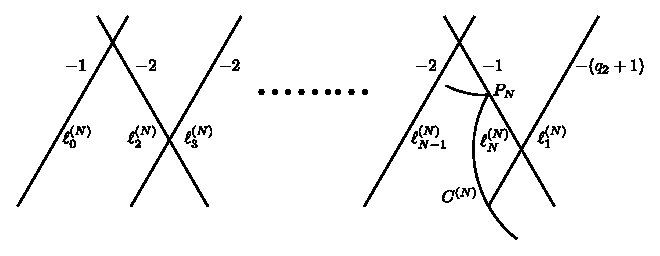
\includegraphics{figures/chap2-fig7.eps}
\end{figure}
where $N:=q_{2}+1$, $P_{N}:=\ell^{(N)}_{N}\cap C^{(N)}$,
$d_{2}=(\ell^{(N)}_{N}\cdot C^{(N)})$ and
$e:=\mult_{P_{N}}C^{(N)}\leqq d_{2}$. Let $\tau_{1}:V_{1}\to V_{0}$ be
the quadratic transformation with center at $Q_{0}:=P_{N}$ and let
$Q_{1}$ be a point on $\tau^{-1}_{1}(P_{N})$ other than the points
$\tau'_{1}(C^{(N)})\cap \tau^{-1}_{1}(Q_{0})$ and
$\tau'_{1}(\ell^{(N)}_{N})\cap \tau^{-1}_{1}(Q_{0})$. For $2\leqq
i\leqq q_{2}-1$, define $\tau_{i}:V_{i}\to V_{i-1}$ and a point
$Q_{i}$ inductively as follows: $\tau_{i}:V_{i}\to V_{i-1}$ is the
quadratic transformation with center at $Q_{i-1}$, and $Q_{i}$ is a
point on $\tau^{-1}_{i}(Q_{i-1})$ other than the point
$\tau'_{i}(\tau^{-1}_{i-1}(Q_{i-2}))\cap \tau^{-1}_{i}(Q_{i-1})$. Let
$\tau_{q_{2}}:W:=V_{q_{2}}\to V_{q_{2}-1}$ be the\pageoriginale\
quadratic transformation with center at $Q_{q_{2}-1}$. Let
$\tau:=\tau_{1}\ldots \tau_{q_{2}}$, let
$L_{i}:=\tau'(\ell^{(N)}_{i})$ for $0\leqq i\leqq N$, let
$E_{j}(1\leqq j\leqq q_{2})$ be the proper transform of
$\tau^{-1}_{j}(Q_{j-1})$ on $W$, and let
$\overline{C}:=\tau'(C^{(N)})$. We have then the following
configuration:
\begin{figure}[H]
\centering
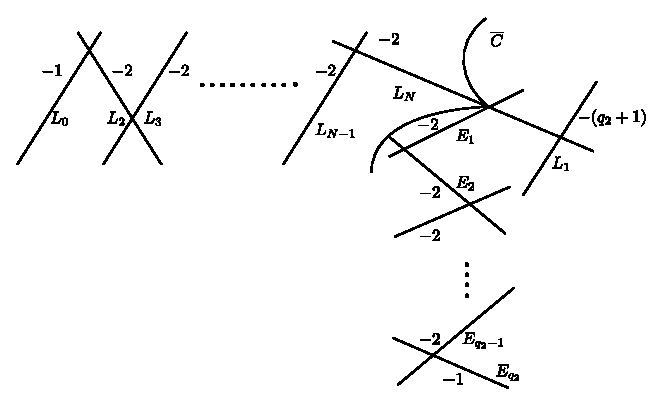
\includegraphics{figures/chap2-fig8.eps}
\end{figure}
where $(\overline{C}\cdot L_{N})=d_{2}-e$ and $(\overline{C}\cdot
E_{1})=e$. Let $\varphi:W\to \mathbb{P}^{2}_{k}$ be the contraction of
curves
$L_{0},L_{2},\ldots,L_{N-1},L_{N},E_{1},E_{2},\ldots,E_{q_{2}-1}$ and
$L_{1}$ in this order, let $\ell'_{0}:=\varphi(E_{q_{2}})$ and let
$C':=\varphi(\overline{C})$. Then a birational automorphism
$\varphi\cdot (\sigma\tau)^{-1}$ is biregular on $\mathbb{A}^{2}_{k}$;
indeed, $\varphi\cdot (\sigma\tau)^{-1}|_{\mathbb{A}^{2}_{k}}$ is a de
Jonqui\`ere transformation $\varphi_{0}$ of $\mathbb{A}^{2}_{k}$ of
degree $N$ (\cf \ref{chap2:3.4.1}). By a straightforward computation we can
easily verify that:
\begin{enumerate}
\renewcommand{\theenumii}{\arabic{enumii}}
\renewcommand{\labelenumii}{(\theenumii)}
\item $C'-(C'\cap \ell'_{0})\cong C_{0}$;

\item $(C'\cdot\ell'_{0})=(q_{2}+1)d_{2}-e=d_{0}-e$;

\item $\mult_{p'}C'=q_{2}d_{2}-e=d_{1}-e$, where $P'_{0}:=C'\cap \ell'_{0}$.
\end{enumerate}
Let $\epsilon':\varphi_{0}\cdot\epsilon:C_{0}\to\mathbb{A}^{2}_{k}$. Then
$\epsilon'$ is an embedding of $C_{0}$ into
$\mathbb{A}^{2}_{k}$\pageoriginale\ with $(C'\cdot
\ell'_{0})=d_{0}-e<d_{0}$ and $\mult_{P'_{0}}C'=d_{1}-e<d_{1}$. By
induction on $d_{0}$, we can show that there exists a
birational automorphism $\rho$ of $\mathbb{P}^{2}_{k}$, which induces a
biregular automorphism $\rho_{0}$ of $\mathbb{A}^{2}_{k}$, such that,
with respect to an embedding $\rho_{0}\cdot \epsilon:C_{0}\to
\mathbb{A}^{2}_{k'}$ either one of the conditions (i) $\sim$ (iii)
holds or $\alpha=1$ and $q_{1}=2$. In the latter case $d_{0}$ becomes
smaller than the original one.

\item {\bf Case:} $\alpha=1$ and $q_{1}=2$. Let $\sigma:V_{0}\to
  \mathbb{P}^{2}_{k}$ be the Euclidean transformation of
  $\mathbb{P}^{2}_{k}$ associated with an admissible datum
  $\{\mathbb{P}^{2}_{k},\mathbb{A}^{2}_{k}, C$, $\ell_{0},\phi,d_{0},d_{1},1\}$. Since
  $d_{0}=2d_{1}$ we have the following configuration of
  $\sigma^{-1}(\ell_{0}\cup C)$:
\begin{figure}[H]
\centering
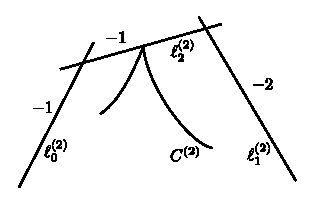
\includegraphics{figures/chap2-fig9.eps}
\end{figure}
Then by the same argument as in step (II) we can show the existence of
a birational automorphism $\rho$ of $\mathbb{P}^{2}_{k}$, which
induces a biregular automorphism $\rho_{0}$ of $\mathbb{A}^{2}_{k}$,
such that, with respect to an embedding
$\rho_{0}\cdot\epsilon:C_{0}\to \mathbb{A}^{2}_{k}$, either one of the
conditions (i) $\sim$ (iii) holds or $\alpha=2$ and $q_{1}=1$ with
$d_{0}$ smaller than the original one.

\item By steps (I) and (II) we can show the existence of a birational
  automorphism $\rho$ as claimed in Lemma.
\end{enumerate}
\end{proof}

\subsection{}\label{chap2:4.2}
With the notations and assumptions of \ref{chap2:4.1}, choose an embedding
$\epsilon:C_{0}\to \mathbb{A}^{2}_{k}$ for which one of the conditions
(i) $\sim$ (iii) of Lemma\pageoriginale\ \ref{chap2:4.1} holds. Let
$\sigma:V_{0}\to \mathbb{P}^{2}_{k}$ be the Euclidean transformation
of $\mathbb{P}^{2}_{k}$ associated with an admissible datum
$\mathscr{D}:=\{\mathbb{P}^{2}_{k},\mathbb{A}^{2}_{k},C,\ell_{0},\phi,d_{0},d_{1},1\}$
for $(\mathbb{A}^{2}_{k},\epsilon(C_{0}))$. Then, looking at the
weighted graph of $\sigma^{-1}_{(\ell_{0})}$ (\cf Figure 1 of
\ref{chap2:1.3.4} as well as the figures given in the proof of Lemma
\ref{chap2:3.1}), we know that $\sigma^{-1}(\ell_{0})$ has an
exceptional curve of the first kind other than $E(\alpha,q_{\alpha})$
if and only if $\alpha\geqq 3$ and $q_{1}=1$. When $\alpha\geqq 3$ and
$q_{1}=1$, by virtue of \ref{chap2:1.3.4}, \ref{chap2:1.4} and \ref{chap2:1.5} we can
readily show the following assertions:
\begin{enumerate}
\renewcommand{\labelenumi}{\theenumi$^{\circ}$}
\item The curves $E_{0}:=\sigma'(\ell_{0})$,
  $E(2,1),\ldots, E(2,q_{2}-1)$ can be contracted successively in this
  order; let $\tau:V_{0}\to V$ be the contraction of these curves.

\item $(\tau(E(2,q_{2}))^{2})=-(q_{3}+1)\leqq -2$ if $\alpha\geqq 4$
  and $(\tau(E(2,q_{2}))^{2})=-q_{3}\leqq -2$ if $\alpha=3$.

\item $a_{0}=a(2,1)=\ldots=a(2,q_{2})=d_{0}$.

\item Let $\overline{C}:=\tau(C^{(N)})$,
  $\overline{\ell}_{0}:=\tau(\ell^{(N)}_{N})$,
  $\overline{E}(s,t):=\tau(E(s,t))$ for $1\leqq s\leqq \alpha$,
  $1\leqq t\leqq q_{s}$ and $(s,t)\neq (2,1),\ldots,(2,q_{2}-1)$,
  $\overline{d}_{0}:=d_{\alpha}$, $\overline{d}_{1}:=$ the
  multiplicity of $\overline{C}$ at the point $\overline{C}\cap
  \overline{\ell}_{0}$,
  $\overline{e}:=a(\alpha,q_{\alpha})/d_{\alpha}$, and
$$
\overline{\Gamma}:=(d_{0}/d_{\alpha})\overline{E}(2,q_{2})+\sum^{\alpha}_{\substack{s=1\\ s\neq
2}}\sum^{q_{s}}_{t=1}(a(s,t)/d_{\alpha})\overline{E}(s,t)-\overline{e}\overline{\ell}_{0}.
$$
Then
$\overline{\mathscr{D}}:=\{V,\mathbb{A}^{2}_{k},\overline{C},\overline{\ell}_{0},\overline{\Gamma},\overline{d}_{0},\overline{d}_{1},\overline{e}\}$
is an admissible datum for $(\mathbb{A}^{2}_{k},\epsilon(C_{0}))$ such
that $\Supp(\overline{\Gamma})$ has no exceptional components and that
the divisor $\overline{d}_{0}(\overline{e\ell}_{0}+\overline{\Gamma})$
contains $\overline{E}(2,q_{2})$ with multiplicity $d_{0}$. 
\end{enumerate}

\subsection{}\label{chap2:4.3}
Assume that an embedding $\epsilon:C_{0}\to \mathbb{A}^{2}_{k}$ is
chosen so that one of the conditions (i) $\sim$ (iii) of Lemma
\ref{chap2:4.1} holds. Define an irreducible\pageoriginale\ linear pencil
$\Lambda$ as follows; if $\alpha\leqq 2$ or $q_{1}\geqq 2$, $\Lambda$
is the linear pencil on $\mathbb{P}^{2}_{k}$ spanned by $C$ and
$d_{0}\ell_{0}$; if $\alpha\geqq 3$ and $q_{1}=1$, $\Lambda$ is the
linear pencil on $V$ spanned by $\overline{C}$ and
$\overline{d}_{0}(\overline{e\ell}_{0}+\overline{\Gamma})$. Now
eliminating the base points of $\Lambda$ by a succession of the
Euclidean transformations and the $(e,i)$-transformations associated
with suitable admissible data for
$(\mathbb{A}^{2}_{k},\epsilon(C_{0}))$, we obtain a nonsingular
projective surface $W$ and a surjective morphism $f:W\to
\mathbb{P}^{1}_{k}$ such that:
\begin{enumerate}
\renewcommand{\labelenumi}{\theenumi$^{\circ}$}
\item The fibers of $f$ are irreducible, except only one fiber
  $\Delta$ which corresponds to the member $d_{0}\ell_{0}$ (or
  $\overline{d}_{0}(\overline{e\ell}_{0}+\overline{\Gamma})$) of
  $\Lambda$.

\item General fibers of $f$ are nonsingular curves of genus $g$, where
  $g$ is the genus of the given curve $C_{0}$.

\item $f$ is a relatively minimal fibration, \iec each fiber does not
  contain exceptional components.

\item If $\Delta:={\displaystyle{\mathop{\sum}^{r}_{i=1}}}n_{i}C_{i}$
  with irreducible components $C_{i}$ and integers $n_{i}>0$ then the
  greatest common divisor of $n_{1},\ldots,n_{r}$ is equal to $1$ and
  at least one of $n_{i}$'s is equal to $d_{0}$.

[For the proof of the assertions $1^{\circ}$ and $2^{\circ}$, see
  Corollary \ref{chap2:1.10} and Lemma \ref{chap2:1.11}; for the proof of
  the assertion $3^{\circ}$, see Lemmas \ref{chap2:1.5} and \ref{chap2:1.7};
  the assertion $4^{\circ}$ follows from the choice of $\Lambda$ and
  the fact that $f$ has a regular cross-section.] 
\end{enumerate}

\subsection{}\label{chap2:4.4}
According to Artin-Winters \cite{7}, we shall call any collection $T$
of integers
$$
T:=\{r,m_{ij},k_{i},n_{i};i,j=1,\ldots,r\},
$$
up\pageoriginale\ to permutation of indices, {\em a fiber type of
  genus} $g$ if there exist a nonsingular projective surface $V$
defined over $k$, a surjective morphism $f$ of $V$ onto a nonsingular
complete curve $B$ whose general members are nonsingular irreducible
curves of genus $g$, and a reducible fiber $\Delta$ of $f$ such that: 
\begin{enumerate}
\renewcommand{\labelenumi}{(\theenumi)}
\item $\Delta:={\displaystyle{\mathop{\sum}^{r}_{i=1}}}n_{i}C_{i}$,
  $C_{i}$ being its irreducible component,

\item $m_{ij}=(C_{i}\cdot C_{j})$ and $k_{i}=(C_{i}\cdot K_{V})$ for
  $i$, $j=1,\ldots,r$, where $K_{V}$ is a canonical divisor of $V$.
\end{enumerate}
The integers $n_{i}$ are called the {\em multiplicities} of a fiber
type $T$ of genus $g$. A fiber type
$T=\{r,m_{ij},k_{i},n_{i};i,j=1,\ldots,r\}$ of genus $g$ is called
{\em relatively minimal} if $m_{ii}\neq -1$ or $k_{i}\neq -1$ for
$i=1,\ldots,r$; $T$ is called {\em reduced} if the greatest common
divisor of $n_{1},\ldots,n_{r}$ is equal to $1$. Now we can state the
following results.

\subsubsection{}\label{chap2:4.4.1}
\begin{lemma*}[(Artin-Winters {[7; Cor.\@ 1.7]}) ]
  Assume that $g\geqq 2$. Then there exists an integer $N(g)$ depending
  only on $g$ such that the multiplicities $n_{i}\leqq N(g)$ for every
  relatively minimal fiber type
  $T=\{r,m_{ij},k_{i},n_{i};i,j=1,\ldots,r\}$ of genus $g$.
\end{lemma*}

\subsubsection{}\label{chap2:4.4.2} 
\begin{lemma*}[(Kodaira {[29; p.\@ 123]}, \v{S}afarevi\v{c} {[51;
      p.171]}) ]
  Assume that $g=1$. Then the multiplicities $n_{i}\leqq 6$ for every
  reduced relatively minimal fiber type
  $T=\{r,m_{ij},k_{i},n_{i};i,j=1,\ldots,r\}$ of genus $1$.
\end{lemma*}

\subsection{}\label{chap2:4.5}
As a consequence of the observations made in the paragraphs \ref{chap2:4.3}
and \ref{chap2:4.4}, we have:

\begin{theorem*}
Let\pageoriginale\ the notations and assumptions be as in
\ref{chap2:4.1}. Assume that $g>0$. Then there are only finitely many
possible pairs $(d_{0},d_{1})$, for each of which there exists an
embedding $\epsilon:C_{0}\to \mathbb{A}^{2}_{k}$ such that
$d_{0}=(C\cdot \ell_{0})$ and $d_{1}=\mult_{P_{0}}C$ {\em (\cf
  \ref{chap2:4.1})} and that one of the conditions {\em (i)} $\sim$ {\em
  (iii)} of Lemma \ref{chap2:4.1} holds.
\end{theorem*}

\begin{proof}
By virtue of the assertion $4^{\circ}$ of \ref{chap2:4.3}, the singular
fiber $\Delta$ has an irreducible component whose multiplicity in
$\Delta$ is $d_{0}$. Then Lemmas \ref{chap2:4.4.1} and \ref{chap2:4.4.2}
imply that there are finitely many possible values of $d_{0}$ (and
therefore, of $d_{1}$ because $0<d_{1}<d_{0}$).
\end{proof}

\subsection{}\label{chap2:4.6}
In the remaining paragraphs of this section we shall prove the
following:

\begin{theorem*}
Let the notations and assumptions be as in \ref{chap2:4.1}. Assume that
$q>0$. Then there are finitely many embeddings $\epsilon:C_{0}\to
\mathbb{A}^{2}_{k}$, up to biregular automorphisms of
$\mathbb{A}^{2}_{k}$, such that:
\begin{enumerate}
\renewcommand{\labelenumi}{\rm(\theenumi)}
\item The curve $C$ ($:=$ the closure of $\epsilon(C_{0})$ in
  $\mathbb{P}^{2}_{k}$) is smoothable by the Euclidean transformation
  of $\mathbb{P}^{2}_{k}$ associated with an admissible datum
  $\{\mathbb{P}^{2}_{k},\mathbb{A}^{2}_{k},
  C,\ell_{0},\phi,d_{0},d_{1},1\}$ for
  $(\mathbb{A}^{2}_{k},\epsilon(C_{0}))$. 

\item One of the following conditions holds:
\begin{enumerate}
\renewcommand{\theenumii}{\roman{enumii}}
\renewcommand{\labelenumii}{\rm(\theenumii)}
\item $\alpha=2$ and $q_{1}\geqq 2$; 

\item $\alpha=1$ and $q_{1}\geqq 3$.
\end{enumerate}
More precisely, if two embeddings $\epsilon$, $\epsilon':C_{0}\to
\mathbb{A}^{2}_{k}$ satisfying the conditions $(1)$ and $(2)$ above
have the same value of $d_{0}$ then there exists an affine
automorphism $\rho_{0}$ of $\mathbb{A}^{2}_{k}$ such that
$\epsilon'=\rho_{0}\cdot \epsilon$. We\pageoriginale\ shall note that
this result is a special case of Finiteness Theorem due to
Abhyankar-Singh \cite{3}; we also note that the condition $(1)$ above is
fulfilled if $\text{G.C.D.}(d_{0},d_{1})=1$.
\end{enumerate}
\end{theorem*}

\subsection{}\label{chap2:4.7}
Let $\epsilon:C_{0}\to \mathbb{A}^{2}_{k}$ be an embedding of $C_{0}$
into $\mathbb{A}^{2}_{k}$ for which the condition $(2)$ above
holds. Let $\sigma:V_{0}\to \mathbb{P}^{2}_{k}$ be the Euclidean
transformation of $\mathbb{P}^{2}_{k}$ associated with the admissible
datum
$\{\mathbb{P}^{2}_{k},\mathbb{A}^{2}_{k},C,\ell_{0},\phi,d_{0},d_{1},1\}$
for $(\mathbb{A}^{2}_{k},\epsilon(C_{0}))$, let $C':=\sigma'(C)$ and
let $\ell$ be a line on $\mathbb{P}^{2}_{k}$ different from the line
$\ell_{0}:=\mathbb{P}^{2}_{k}-\mathbb{A}^{2}_{k}$. Then we have:

\begin{lemma*}
With the notations as above and as in \ref{chap2:1.3.4}, we have:
$$
C'-\sigma^{\ast}(\ell)\sim (d_{0}-d_{1}-1)\sigma^{\ast}(\ell)+\Delta,
$$
where
$$
\Delta:=
\begin{cases}
d_{1}E_{0} & \text{if } \alpha =1,\\
d_{1}E_{0}+\sum^{r}_{i=1}\sum^{q_{2i}}_{t=1}(d_{2i-1}-td_{2i})E(2i,t)
& \text{if } \alpha=2r\text{ \  and \ }r\geqq 1,\\
d_{1}E_{0}+\sum^{r}_{i=1}\sum^{q_{2i}}_{t=1}(d_{2i-1}-td_{2i})E(2i,t)
& \text{if } \alpha=2r+1 \text{ \  and \ } r\geqq 1.
\end{cases}
$$
\end{lemma*}

\begin{proof}
By virtue of Lemma \ref{chap2:1.5} and its proof, we have:
\begin{gather*}
C'\sim d_{0}E_{0}+\sum^{\alpha}_{s=1}\sum^{q_{s}}_{t=1}a(s,t)E(s,t)\\
\sigma^{\ast}(\ell)\sim
\sigma^{\ast}(\ell_{0})=E_{0}+\sum^{\alpha}_{s=1}\sum^{q_{2s}}_{t=1}c(s,t)E(s,t), 
\end{gather*}
where the integers $a(s,t)$ and $c(s,t)$ are defined in
\ref{chap2:1.4}. Hence we have:
$$
C'-(d_{0}-d_{1})\sigma^{\ast}(\ell)\sim
d_{1}E_{0}+\sum^{\alpha}_{s=1}\sum^{q_{s}}_{t=1}b(s,t)E(s,t), 
$$\pageoriginale\
where $b(s,t):=a(s,t)-(d_{0}-d_{1})c(s,t)$ is defined as follows:
\begin{alignat*}{2}
b(1,t) &= (d_{0}-d_{1})t-(d_{0}-d_{1})t=0\qquad & \text{for } 1\leqq
t\leqq q_{1}\\
b(2,t) &= d_{1}+t(b(1,q_{1})-d_{2})=d_{1}-td_{2}  &\text{for } 1\leqq
t\leqq q_{2}, \\
 &\quad \ldots\ldots\ldots\ldots & \\
b(s,t) &= b(s-2,q_{s-2})+t(b(s-1,q_{s-1})-d_{s}) &\text{for } 1\leqq
t\leqq q_{s}\\ 
 & & \text{and } 2\leqq s\leqq \alpha.
\end{alignat*}
Thence we have: $b(2i,t)=d_{2i-1}-td_{2i}$ for $1\leqq i\leqq r$ and
$1\leqq t\leqq q_{2i}$, and $b(2i+1,t)=0$ for $0\leqq i\leqq
r(2i+1\leqq \alpha)$ and $1\leqq t\leqq q_{2i+1}$, where
$r=\left[\dfrac{\alpha}{2}\right]$. Thus we obtain our
assertion.
\end{proof}

\subsection{}\label{chap2:4.8}
According to Ramanujam \cite{46}, an effective divisor $D$ on a
nonsingular projective surface $V_{0}$ defined over $k$ is called {\em
  numerically connected} if for every decomposition $D=D_{1}+D_{2}$
with $D_{i}>0(i=1,2)$ we have $(D_{1}\cdot D_{2})>0$. We shall show:

\begin{lemma*}
The divisor $(d_{0}-d_{1}-1)\sigma^{\ast}(\ell)+\Delta$ is numerically
connected provided $q_{1}\geqq 2$.
\end{lemma*}

A proof of the lemma will be given in the subparagraphs \ref{chap2:4.8.1}
$\sim$ \ref{chap2:4.8.3}.

\subsubsection{}\label{chap2:4.8.1}
\begin{lemma*}
  Let $D$ be an effective divisor on a nonsingular projective surface
  $V$ defined over $k$. Write
  $D:={\displaystyle{\mathop{\sum}^{r}_{i=1}}}m_{i}D_{i}$ with
  irreducible components $D_{i}$ and integers $m_{i}>0$. Assume that
  $(D^{2}_{i})=-\alpha_{i}$ for $1\leqq i\leqq r$ and $(D_{i}\cdot
  D_{j})=\delta_{j,i+1}$ {\em (Kronecker's delta)} for\pageoriginale\
  $1\leqq i$, $j\leqq r$ and $i\neq j$. Let
  $D_{1}:={\displaystyle{\mathop{\sum}^{r}_{i=1}}}x_{i}D_{i}$ with
  $0\leqq x_{i}\leqq m_{i}(1\leqq i\leqq r)$, and let
  $D_{2}:=D-D_{1}$. Then we have:
  \begin{multline*}
    (D_{1}\cdot D_{2}) =
    (\alpha_{1}-1)x^{2}_{1}+\sum^{r-1}_{i=2}(\alpha_{i}-2)x^{2}_{i} +
    (\alpha_{r}-1)x^{2}_{r}+\sum^{r-1}_{i=1}(x_{i}-x_{i+1})^{2}\\  
    +(m_{2}-\alpha_{1}m_{1})x_{1}+\sum^{r-1}_{i=2}(m_{i-1}-
    \alpha_{i}m_{i}+m_{i+1})x_{i}+(m_{r-1}-\alpha_{r}m_{r})x_{r}.  
  \end{multline*}
\end{lemma*}

\begin{proof}
A straightforward computation.
\end{proof}

\subsubsection{}\label{chap2:4.8.2}
\begin{lemma*}
  With the notations as in \ref{chap2:4.7}, let
  $D:=(d_{0}-d_{1}-1)\sigma^{\ast}(\ell)+\Delta$ and let
  $$
  D_{1}:=y\sigma^{\ast}(\ell)+x_{0}E_{0}+\sum^{r}_{i=1}
  \sum^{q_{2i}}_{t=1}x(2i,j) E(2i,j)\quad\text{and}\quad D_{2}:=D-D_{1}, 
  $$
  where we assume that $D_{i}>0$ for $i=1,2$. Then we have:
  $$
  (D_{1}\cdot
  D_{2})=-2y^{2}+(q_{1}-2)x^{2}_{0}+(x_{0}-y)^{2}+(d_{0}-1)y-x_{0}+Q 
  $$
  where $Q:=0$ if $\alpha=1$;
  \begin{align*}
    Q: &= \sum^{r-1}_{i=1}q_{2i+1}x(2i,q_{2i})^{2}+x(2r,q_{2r}-1)^{2}\\
    &\quad +\{(x_{0}-x(2,1))^{2}+\sum^{q_{2}-1}_{t=1}(x(2,t)-x(2,t+1))^{2}\}\\
    & + \sum^{r-1}_{i=2}\left\{(x(2i-2,q_{2i-2})-x(2i,1))^{2} +
    \sum^{q_{2i}-1}_{t=1}(x(2i,t)-x(2i,t+1))^{2}\right\}\\ 
    &\quad + \left\{(x(2r-2,q_{2r-2})-x(2r,1))^{2} + \sum^{q_{2r}-2}_{t=1}
    (x(2r,t)-x(2r,t+1))^{2}\right\}  
  \end{align*}
  if $\alpha=2r$ and $r\geqq 1$;
  \begin{align*}
    Q: &=\sum^{r}_{i=1}q_{2i+1}x(2i,q_{2i})^{2}+\{(x_{0}-x(2,1))^{2}+
    \sum^{q_{2}-1}_{t=1}(x(2,t)-x(2,t+1))^{2}\}\\  
    &\quad +\sum^{r}_{i=2}\{(x(2i-2,q_{2i-2})-x(2i,1))^{2}+
    \sum^{q_{2i}-1}_{t=1}(x(2i,t)-x(2i,t+1))^{2}\}  
  \end{align*}
  if\pageoriginale\ $\alpha=2r+1$ and $r\geqq 1$.
\end{lemma*}

\begin{proof}
  Note that $(\sigma^{\ast}(\ell)^{2})=1$, $(\sigma^{\ast}(\ell)\cdot
  E_{0})=1$ and $(\sigma^{\ast}(\ell)\cdot E(2i,t))=0$ for $1\leqq
  i\leqq r$ and $1\leqq t\leqq q_{2i}$. Then we obtain our assertion by
  applying Lemma \ref{chap2:4.8.1} and taking account of \ref{chap2:1.3.3} and
  \ref{chap2:1.3.4}.
\end{proof}

\subsubsection{}\label{chap2:4.8.3}
\begin{proofoflemma*}[4.8 ]
  Regarding $(D_{1}\cdot D_{2})$ as a function of variables $y$, $x_{0}$
  and $x(2i,t)$'s, we shall estimate the smallest value of $(D_{1}\cdot
  D_{2})$ when the variables $y$, $x_{0}$ and $x(2i,t)$'s take integral
  values in the domain $A$:
  \begin{align*}
    & 0\leqq y\leqq d_{0}-d_{1}-1;\quad 0\leqq x_{0}\leqq d_{1};\quad
    0\leqq x(2i,t)\leqq d_{2i-1}-td_{2i}\\
    & (1\leqq i\leqq r; 1\leqq t\leqq q_{2i}).
  \end{align*}
  By virtue of Lemma \ref{chap2:4.8.2}, $(D_{1}\cdot D_{2})$ is written in
  the form:
  $$
  (D_{1}\cdot D_{2})=-y^{2}+(d_{0}-1-2x_{0})y+(q_{1}-1)x^{2}_{0}-x_{0}+Q,
  $$
  which, viewed as a function in $y$ only, has the smallest value at
  $y=0$ or $y=d_{0}-d_{1}-1$ whenever values of $x_{0}$ and $x(2i,t)$'s
  $(1\leqq i\leqq r; 1\leqq t\leqq q_{2i})$ are fixed in the domain
  $A$. If $y=0$ we have:
  $$
(D_{1}\cdot D_{2})=x_{0}\{(q_{1}-1)x_{0}-1\}+Q.
  $$
  Consider first the case where $\alpha=1$. Then $q_{1}\geqq 3$ as
  assumed. Since $D_{1}>0$, \iec $x_{0}\neq 0$ and $x_{0}$ takes an
  integral value, we know\pageoriginale\ that 
  $(D_{1}\cdot D_{2})>0$ for $0<x_{0}\leqq d_{1}$. Assume that
  $\alpha\geqq 2$. Since $q_{1}\geqq 2$ as assumed and $x_{0}$ takes an
  integral value, we know that $(D_{1}\cdot D_{2})\geqq Q\geqq 0$, and
  that $(D_{1}\cdot D_{2})=Q$ if and only if either $x_{0}=0$ or
  $q_{1}=2$ and $x_{0}=1$. Besides, by virtue of Lemma \ref{chap2:4.8.2},
  $Q=0$ if and only if $x_{0}=x(2i,t)=0$ for $1\leqq i\leqq r$ and
  $1\leqq t\leqq q_{2i}$. Therefore we have $(D_{1}\cdot D_{2})>0$
  because $D_{1}>0$. If $y=d_{0}-d_{1}-1$ we obtain $(D_{1}\cdot
  D_{2})>0$ by interchanging the roles of $D_{1}$ and $D_{2}$. Hence
  $(D_{1}\cdot D_{2})>0$ for every decomposition $D=D_{1}+D_{2}$ with
  $D_{i}>0(i=1,2)$. This completes a proof of Lemma \ref{chap2:4.8}.
\end{proofoflemma*}

\subsection{}\label{chap2:4.9}
We shall next consider the case where $q_{1}=1$ and $\alpha\geqq
3$. We shall use the notations of the paragraph \ref{chap2:4.2}. Thus,
$\tau:V_{0}\to V$ is the contraction of curves $E_{0}$,
$E(2,1),\ldots,E(2,q_{2}-1)$. Let $L:=\tau_{\ast}\sigma^{\ast}(\ell)$
and $\overline{E}_{0}:=\overline{E}(2,q_{2})$.

\subsubsection{}\label{chap2:4.9.1}
\begin{lemma*}
  We have: $\overline{C}-L\sim(d_{2}-1)L+\overline{\Delta}$, where
  $$
  \overline{\Delta}:=
  \begin{cases}
    d_{3}\overline{E}_{0} & \text{if }\alpha=3,\\
    d_{3}\overline{E}_{0}
    +\sum^{r}_{i=2}\sum^{q_{2i}}_{t=1}(d_{2i-1}-td_{2i})\overline{E}(2i,t)
    & \text{if } \alpha\geqq 4.
  \end{cases}
  $$
\end{lemma*}

\begin{proof}
Immediate from Lemma \ref{chap2:4.7}.
\end{proof}

\subsubsection{}\label{chap2:4.9.2}
\begin{lemma*}
  Let $\overline{D}:=(d_{2}-1)L+\overline{\Delta}$ and let
  $$
  \overline{D}_{1}:=\overline{y}L+\overline{x}_{0}\overline{E}_{0}+\sum^{r}_{i=2}\sum^{q_{2i}}_{t=1}\overline{x}(2i,t)\overline{E}(2i,t)\quad\text{and}\quad
  \overline{D}_{2}:=\overline{D}-\overline{D}_{1}, 
  $$
  where we assume that $\overline{D}_{i}>0$ for $i=1,2$. Then we have:
  $$
  (\overline{D}_{1}\cdot
  \overline{D}_{2})=-(q_{2}+2)\overline{y}^{2}+(q_{3}-1)\overline{x}^{2}_{0}+(\overline{x}_{0}-\overline{y})^{2}+(d_{0}-(q_{2}+1))\overline{y}-\overline{x}_{0}+\overline{Q}, 
  $$
  where\pageoriginale\
  \begin{align*}
    \overline{Q} &:= 0 \text{ \  if \ }\alpha=3;\\
    \overline{Q} &:=
    \sum^{r-1}_{i=2}q_{2i+1}\overline{x}(2i,q_{2i})^{2}+\overline{x}
    (2r,q_{2r}-1)^{2}\\ 
    &\quad +\{(\overline{x}_{0}-\overline{x}(4,1))^{2} +
    \sum^{q_{4}-1}_{t=1}(\overline{x}(4,t)-\overline{x}(4,t+1))^{2}\}\\ 
    &\quad +\sum^{r-1}_{i=3}\{(\overline{x}(2i-2,q_{2i-2})-
    \overline{x}(2i,1))^{2}+\sum^{q_{2i}-1}_{t=1} (\overline{x}(2i,t)
    - \overline{x}(2i,t+1))^{2}\}\\ 
    &\quad +\{(\overline{x}(2r-2,q_{2r-2})- \overline{x}(2r,1))^{2} +
    \sum^{q_{2r}-2}_{t=1}(\overline{x}(2r,t)-\overline{x}(2r,t+1))^{2}\} 
  \end{align*}
  if $\alpha=2r\geqq 4$;
  \begin{align*}
    \overline{Q} &:=
    \sum^{r}_{i=2}q_{2i+1}\overline{x}(2i,q_{2i})^{2}+\{(\overline{x}_{0}
    - \overline{x}(4,1))^{2}+\sum^{q_{4}-1}_{t=1}(\overline{x}(4,t) -
    \overline{x}(4,t+1))^{2}\}\\ 
    &\quad
    +\sum^{r}_{i=3}\{(\overline{x}(2i-2,q_{2i-2})-\overline{x}(2i,1))^{2}+\sum^{q_{2i}-1}_{t=1}(\overline{x}(2i,t)-\overline{x}(2i,t+1))^{2}\} 
  \end{align*}
  if $\alpha=2r+1\geqq 4$.
\end{lemma*}

\begin{proof}
Note that $(L^{2})=q_{2}+1$, $(L\cdot\overline{E}_{0})=1$, $(L\cdot
\overline{E}(2i,t))=0$ for $2\leqq i\leqq r$ and $1\leqq t\leqq
q_{2i}$, and $(\overline{E}^{2}_{0})=-q_{3}$ if $\alpha=3$ and
$(\overline{E}^{2}_{0})=-(q_{3}+1)$ if $\alpha\geqq 4$. Then our
assertion follows from Lemma \ref{chap2:4.8.1}.
\end{proof}

\subsubsection{}\label{chap2:4.9.3}
\begin{lemma*}
  The divisor $\overline{D}:=(d_{2}-1)L+\overline{\Delta}$ is
  numerically connected.
\end{lemma*}

\begin{proof}
Regarding $(\overline{D}_{1}\cdot \overline{D}_{2})$ as a function of
variables $\overline{y}$, $\overline{x}_{0}$ and
$\overline{x}(2i,t)$'s $(2\leqq i\leqq r;1\leqq t\leqq q_{2i})$, we
shall estimate the smallest value of $(\overline{D}_{1}\cdot
\overline{D}_{2})$ when the variables $\overline{y}$,
$\overline{x}_{0}$ and $\overline{x}(2i,t)$'s take integral values in
the domain $\overline{A}$:
$$
0\leqq \overline{y}\leqq d_{2}-1;\quad 0\leqq \overline{x}_{0}\leqq
d_{3};\quad 0\leqq \overline{x}(2i,t)\leqq d_{2i-1}-td_{2i}
$$\pageoriginale\
for $2\leqq i\leqq r$ and $1\leqq t\leqq q_{2i}$.

By virtue of Lemma \ref{chap2:4.9.2}, $(\overline{D}_{1}\cdot
\overline{D}_{2})$ is written in the form:
$$
(\overline{D}_{1}\cdot
\overline{D}_{2})=-(q_{2}+1)\overline{y}^{2}+\{d_{0}-(q_{2}+1)-2\overline{x}_{0}\}\overline{y}+q_{3}\overline{x}^{2}_{0}-\overline{x}_{0}+\overline{Q}, 
$$
which, viewed as a function only in $\overline{y}$, has the smallest
value at $\overline{y}=0$ or $\overline{y}=d_{2}-1$. If
$\overline{y}=0$ we have:
$$
(\overline{D}_{1}\cdot
\overline{D}_{2})=\overline{x}_{0}(q_{3}\overline{x}_{0}-1)+\overline{Q}. 
$$

Since $\overline{x}_{0}$ takes an integral value, we know that
$(\overline{D}_{1}\cdot\overline{D}_{2})\geqq \overline{Q}\geqq 0$. If
$\alpha=3$, then $q_{3}\geqq 2$ and $(\overline{D}_{1}\cdot
\overline{D}_{2})=\overline{x}_{0}(q_{3}\overline{x}_{0}-1)=0$ if and
only if $\overline{x}_{0}=0$, \iec $\overline{D}_{1}=0$. Thus
$(\overline{D}_{1}\cdot \overline{D}_{2})>0$ if $\alpha=3$. Assume
that $\alpha\geqq 4$. Then, by virtue of Lemma \ref{chap2:4.9.2},
$\overline{Q}=0$ if and only if
$\overline{x}_{0}=\overline{x}(2i,t)=0$ for $2\leqq i\leqq r$ and
$1\leqq t\leqq q_{2i}$, \iec $\overline{D}_{1}=0$. Hence
$(\overline{D}_{1}\cdot \overline{D}_{2})>0$. If
$\overline{y}=d_{2}-1$ we obtain $(\overline{D}_{1}\cdot
\overline{D}_{2})>0$ by interchanging the roles of $\overline{D}_{1}$
and $\overline{D}_{2}$. Therefore we know that $(\overline{D}_{1}\cdot
\overline{D}_{2})>0$ for every decomposition
$\overline{D}=\overline{D}_{1}+\overline{D}_{2}$ with
$\overline{D}_{i}>0$ for $i=1,2$.
\end{proof}

\subsection{}\label{chap2:4.10}
\begin{lemma*}
  With the notations of \ref{chap2:4.1}, let $\epsilon:C_{0}\to
  \mathbb{A}^{2}_{k}$ be an embedding such that one of the following
  conditions holds:
  \begin{itemize}
  \item[\rm(i)] $\alpha\geqq 2$ and $q_{1}\geqq 2$;
    
  \item[\rm(ii)] $\alpha=1$ and $q_{1}\geqq 3$.
  \end{itemize}
  Let $\sigma:V_{0}\to \mathbb{P}^{2}_{k}$ be the Euclidean
  transformation of $\mathbb{P}^{2}_{k}$ associated with an admissible
  datum
  $\{\mathbb{P}^{2}_{k},\mathbb{A}^{2}_{k},C,\ell_{0},\phi,d_{0},d_{1},1\}$
  for $(\mathbb{A}^{2}_{k},\epsilon(C_{0}))$, let $C':=\sigma'(C)$ and
  let $\ell$ be a line on $\mathbb{P}^{2}_{k}$ different\pageoriginale\
  from the line $\ell_{0}$. Then we have:
  $$
  \dim_{k}H^{0}(C',\mathscr{O}_{C'}(\sigma^{\ast}(\ell)\cdot C'))=3.
  $$
\end{lemma*}

\begin{proof}
Consider an exact sequence
$$
0\to \mathscr{O}_{V_{0}}(-C'+\sigma^{\ast}(\ell))\to
\mathscr{O}_{V_{0}}(\sigma^{\ast}(\ell))\to
\mathscr{O}_{C'}(\sigma^{\ast}(\ell)\cdot C')\to 0.
$$
Thence we obtain an exact sequence
\begin{align*}
& 0\to H^{0}(V_{0},\mathscr{O}_{V_{0}}(-C'+\sigma^{\ast}(\ell)))\to
  H^{0}(V_{0},\mathscr{O}_{V_{0}}(\sigma^{\ast}(\ell)))\to\\
& H^{0}(C',\mathscr{O}_{C'}(\sigma^{\ast}(\ell)\cdot C'))\to
  H^{1}(V_{0},\mathscr{O}_{V_{0}}(-C'+\sigma^{\ast}(\ell))). 
\end{align*}
By virtue of Lemmas \ref{chap2:4.7} and \ref{chap2:4.8} we know that
$C'-\sigma^{\ast}(\ell)\sim
D:=(d_{0}-d_{1}-1)\sigma^{\ast}(\ell)+\Delta$ and $D$ is numerically
connected. Since $V_{0}$ is a nonsingular projective rational surface
we have: $H^{1}(V_{0},\mathscr{O}_{V_{0}})=(0)$. Hence we have:
$$
\dim_{k}H^{1}(V_{0},\mathscr{O}_{V_{0}}(-D))=\dim_{k}H^{0}(D,\mathscr{O}_{D})-1,
$$
where $\dim_{k}H^{0}(D,\mathscr{O}_{D})=1$ by virtue of Ramanujam's
theorem [46; Lemma 3]. Thus we know that
$H^{1}(V_{0},\mathscr{O}_{V_{0}}(-C'+\sigma^{\ast}(\ell)))=(0)$. Since
$H^{0}(V_{0},\mathscr{O}_{V_{0}}(-C'+\sigma^{\ast}(\ell)))=(0)$
clearly, we obtain:
$$
H^{0}(C',\mathscr{O}_{C'}(\sigma^{\ast}(\ell)\cdot C'))\cong
H^{0}(V_{0},\mathscr{O}_{V_{0}}(\sigma^{\ast}(\ell)))\cong
H^{0}(\mathbb{P}^{2}_{k},\mathscr{O}_{\mathbb{P}^{2}}(1)). 
$$
Therefore we have
$\dim_{k}H^{0}(C',\mathscr{O}_{C'}(\sigma^{\ast}(\ell)\cdot
C'))=3$.
\end{proof}

\begin{remark*}
If $q_{1}=1$ and $\alpha\geqq 3$, let $\tau:V_{0}\to V$ be the
contraction of curves $E_{0}$, $E(2,1),\ldots,E(2,q_{2}-1)$, let
$\overline{C}=\tau(C')$ and let $L:=\tau_{\ast}\sigma^{\ast}(\ell)$
(\cf \ref{chap2:4.9}). Then we obtain:
\begin{align*}
\dim_{k}H^{0}(\overline{C},\mathscr{O}_{\overline{C}}(L\cdot
\overline{C})) &= \dim_{k}H^{0}(V,\mathscr{O_{V}}(L))\geqq
\dim_{k}H^{0}(V_{0},\mathscr{O}_{V_{0}}(\sigma^{\ast}(\ell))\\ 
 &= \dim_{k}H^{0}(\mathbb{P}^{2}_{k},\mathscr{O}_{\mathbb{P}^{2}}(1))=3.
\end{align*}\pageoriginale\
\end{remark*}

\subsection{}\label{chap2:4.11}
\begin{proofoftheorem*}[4.6 ]
  Let $\epsilon:C_{0}\to \mathbb{A}^{2}_{k}$ be an embedding satisfying
  the conditions (1) and (2) as stated in Theorem \ref{chap2:4.6}. With the
  notations of \ref{chap2:4.1} and \ref{chap2:4.7}, we know that:
  \begin{enumerate}
    \renewcommand{\labelenumi}{\theenumi$^{\circ}$}
  \item The curve $C'$ is a normalization of the curve $C$ which is of
    qenux $g>0$; set $\widetilde{C}(\epsilon):=C'$ and
    $\delta(\epsilon):=\sigma^{\ast}(\ell)\cdot C'$.
    
  \item Let $\widetilde{P}(\epsilon)$ be the (unique) point of
    $\widetilde{C}(\epsilon)$ dominating the point $P_{0}$ of $C$. Then
    $\delta(\epsilon)\sim d_{0}\widetilde{P}(\epsilon)$,
    $\delta(\epsilon)$ is an effective divisor such that
    $|\delta(\epsilon)|$ has no base points and
    $\dim|\delta(\epsilon)|=2$ (\cf. Lemma \ref{chap2:4.10}).
    
  \item Let
    $f(\epsilon):\widetilde{C}(\epsilon)\xrightarrow{\pi(\epsilon)}\overline{\epsilon(C_{0})}\hookrightarrow
    \mathbb{P}^{2}_{k}$ be the morphism defined from the embedding
    $\epsilon$, where $\pi(\epsilon):=\sigma|_{C'}$ and where
    $\overline{\epsilon(C_{0})}=C$ is the closure of $\epsilon(C_{0})$
    in $\mathbb{P}^{2}_{k}$. Then $f(\epsilon)$ is a morphism defined by
    $|\delta(\epsilon)|$ with respect to a suitable basis of
    $|\delta(\epsilon)|$.
  \end{enumerate}
  Now, let $\epsilon$ and $\epsilon'$ be embeddings of $C_{0}$ into
  $\mathbb{A}^{2}_{k}$ satisfying the conditions (1) and (2) as stated
  in Theorem \ref{chap2:4.6} and having the same value of $d_{0}$. Then
  $\epsilon'\cdot \epsilon^{-1}:\epsilon(C_{0})\to \epsilon'(C_{0})$
  induces an isomorphism $h:\widetilde{C}(\epsilon)\to
  \widetilde{C}(\epsilon')$ such that
  $h(\widetilde{P}(\epsilon))=\widetilde{P}(\epsilon')$ and
  $(\epsilon'\cdot \epsilon^{-1})\cdot \pi
  (\epsilon)=\pi(\epsilon')\cdot h$ on
  $\widetilde{C}(\epsilon)-\{\widetilde{P}(\epsilon)\}$. Since
  $\delta(\epsilon)\sim d_{0}\widetilde{P}(\epsilon)$ and
  $\delta(\epsilon')\sim d_{0}\widetilde{P}(\epsilon')$, we know that
  $\delta(\epsilon)\sim h^{\ast}\delta(\epsilon')$. This implies by
  virtue of the above assertions $2^{\circ}$ and $3^{\circ}$ that there
  exists a biregular (hence, linear) automorphism $\rho$ of
  $\mathbb{P}^{2}_{k}$ such that $\rho\cdot
  \pi(\epsilon)=\pi(\epsilon')\cdot h$ and $\rho(\ell_{0})=\ell_{0}$; 
  \[
  \xymatrix@C=1.4cm{
    \widetilde{C}(\epsilon)\ar[dd]_{h}\ar[rr]^{\pi(\epsilon)} & &
    \overline{\epsilon(C_{0})}\ar[dd]^{\epsilon'\cdot
      \epsilon^{-1}}\ar@{^{(}->}[rr] && \mathbb{P}^{2}_{k}\ar[dd]^{\rho}\\
    & C_{0}\ar[ur]^{\epsilon}\ar[dr]_{\epsilon'} && & \\
    \widetilde{C}(\epsilon')\ar[rr]_{\pi(\epsilon')} &&
    \overline{\epsilon'(C_{0})}\ar@{^{(}->}[rr] && \mathbb{P}^{2}_{k}
  }
  \]\pageoriginale\
  Let $\rho_{0}=\rho|_{\mathbb{A}^{2}_{k}}$. Then it is
  clear that $\rho_{0}\cdot\epsilon=\epsilon'$. 
\end{proofoftheorem*}


\section{Simple birational extensions of a polynomial ring
  $k[x,y]$}\label{chap2:sec5}\pageoriginale\

\subsection{}\label{chap2:5.1}
Let $k$ be an algebraically closed field of characteristic $p$ and let
$k[x,y]$ be a polynomial ring over $k$ in two variables $x$ and
$y$. Let $f$ and $g$ be two elements of $k[x,y]$ without common
nonconstant factors, and let $A:=k[x,y,f/g]$. In this section we shall
consider the structures of the affine $k$-domain $A$ under an
assumption that $V:=\Spec(A)$ has only isolated singularities. In the
paragraphs \ref{chap2:5.2} $\sim$ \ref{chap2:5.9} we shall describe how $V$ is
obtained from $\mathbb{A}^{2}_{k}:=\Spec(k[x,y])$, and see that if $V$
has only isolated singularities $V$ is a normal surface whose singular
points (if any) are rational double points (\cf Theorem
\ref{chap2:5.9}). The divisor class group $C\ell(V)$ can be explicitly
determined (\cf Theorem \ref{chap2:5.11}); we obtain, therefore,
necessary and sufficient conditions for $A$ to be a unique
factorization domain. If $g$ is irreducible and if the curves $f=0$
and $g=0$ on $\mathbb{A}^{2}_{k}$ meet each other then $A$ is a unique
factorization domain if and only if the curves $f=0$ and $g=0$ meet in
only one point where both curves intersect transversely. We shall
consider, in the paragraphs \ref{chap2:5.13} and \ref{chap2:5.14} a problem: When
is every invertible element of $A$ constant? (\cf Theorem
\ref{chap2:5.14}). In the remaining paragraphs \ref{chap2:5.16} $\sim$
\ref{chap2:5.23}, assuming that $k$ is of characteristic zero, we shall look
for a necessary and sufficient condition for $A$ to have a nontrivial
locally nilpotent $k$-derivation (\cf Theorem \ref{chap2:5.23}). An
affine $k$-domain of type $A$ as above was studied by Russell
\cite{49} and Sathaye \cite{52} in connection with the following
result:\pageoriginale\ 

{\em Assume that $A$ is isomorphic to a polynomial ring over $k$ in
  two variables. In a polynomial ring $k[x,y,z]$ over $k$ in three
  variables $x$, $y$ and $z$, let $u:=gz-f$. Then there exist two
  elements $v$, $w$ of $k[x,y,z]$ such that $k[x,y,z]=k[u,v,w]$.}

\subsection{}\label{chap2:5.2}
Let $k[x,y,z]$ be a polynomial ring over $k$ in three variables $x$,
$y$ and $z$, and let $\mathbb{A}^{3}_{k}:=\Spec(k[x,y,z])$. Let $V$ be
an affine hyper surface on $\mathbb{A}^{3}_{k}$ defined by $gz-f=0$,
and let $\pi:V\to \mathbb{A}^{2}_{k}:=\Spec(k[x,y])$ be the
projection: $\pi(x,y,z)=(x,y)$. Let $F$ and $G$ be respectively the
curves $f=0$ and $g=0$ on $\mathbb{A}^{2}_{k}$. Then we have:

\begin{lemma*}
\begin{enumerate}
\renewcommand{\labelenumi}{\rm(\theenumi)}
\item For each point $P\in F\cap G$, $\pi^{-1}(P)$ is isomorphic to
  the affine line $\mathbb{A}^{1}_{k}$.

\item If $Q$ is a point on $G$ but not on $F$, then
  $\pi^{-1}(P)=\phi$. 
\end{enumerate}
\end{lemma*}

\begin{proof}
Straightforward.
\end{proof}

\subsection{}\label{chap2:5.3}
The Jacobian criterion of singularity applied to the hyper surface $V$
shows us the following:

\begin{lemma*}
Let $P$ be a point on $F$ and $G$. Then the following assertions hold:
\begin{enumerate}
\renewcommand{\labelenumi}{\rm(\theenumi)}
\item If $P$ is a singular point for both $F$ and $G$ then every point
  of $\pi^{-1}(P)$ is a singular point of $V$.

\item If $P$ is a singular point of $F$ but not a singular point of
  $G$ then the point $(P,z=0)$ is the unique singular point of $V$
  lying on $\pi^{-1}(P)$.

\item If\pageoriginale\ $P$ is a singular point of $G$ but not a
  singular point of 
  $F$ then $V$ is nonsingular at every point of $\pi^{-1}(P)$.

\item If $P$ is a nonsingular point of both $F$ and $G$ and if
  $i(F,G;P)\geqq 2$ then the point $(P,z=\alpha)$ is the unique
  singular point of $V$ lying on $\pi^{-1}(P)$, where $\alpha\in k$
  satisfies: $\dfrac{\partial f}{\partial x}(P)=\alpha\dfrac{\partial
    g}{\partial x}(P)$ and $\dfrac{\partial f}{\partial
    y}(P)=\alpha\dfrac{\partial g}{\partial y}(P)$. If $i(F,G;P)=1$
  then $V$ is nonsingular at every point of $\pi^{-1}(P)$.
\end{enumerate}
\end{lemma*}

We assume, from now on, that $V$ has only isolated
singularities. Hence, if $P\in F\cap G$, either $F$ or $G$ is
nonsingular at $P$. Furthermore, we assume that $F\cap G\neq
\phi$. When $F\cap G=\phi$ then $A=k[x,y,1/g]$ and $A$ is a unique
factorization domain. 

\subsection{}\label{chap2:5.4}
Let $P$ be a point on $F$ and $G$. We shall first consider the case
where $F$ is nonsingular at $P$ but $G$ singular at $P$. Let
$P_{1}:=P$ and let $\nu_{1}$ be the multiplicity of $G$ at
$P_{1}$. Let $\sigma_{1}:V_{1}\to V_{0}:=\mathbb{A}^{2}_{k}$ be the
quadratic transformation with center at $P_{1}$, let
$P_{2}:=\sigma'_{1}(F)\cap \sigma^{-1}_{1}(P_{1})$ and let $\nu_{2}$
be the multiplicity of $\sigma'_{1}(G)$ at $P_{2}$. For $i\geqq 1$ we
define a surface $V_{i}$, a point $P_{i+1}$ on $V_{i}$ and an integer
$\nu_{i+1}$ inductively as follows: When $V_{i-1}$, $P_{i}$ and
$\nu_{i}$ are defined, let $\sigma_{i}:V_{i}\to V_{i-1}$ be the
quadratic transformation of $V_{i-1}$ with center at $P_{i-1}$, let
$P_{i+1}:=(\sigma_{1}\ldots\sigma_{i})'(F)\cap \sigma^{-1}_{i}(P_{i})$
and let $\nu_{i+1}$ be the multiplicity of
$(\sigma_{1}\ldots\sigma_{i})'(G)$ at $P_{i+1}$. Let $s$ be the
smallest integer such that $\nu_{s+1}=0$, and let
$N:\nu_{1}+\cdots+\nu_{s}$. We shall simply say that
$P_{1},\ldots,P_{s}$ {\em are all points of $G$ on the curve $F$ over
  $P_{1}$ and $\nu_{1},\ldots,\nu_{s}$ are the respective
  multiplicities of $G$ at $P_{1},\ldots,P_{s}$.} Let $\sigma:V_{N}\to
V_{0}$ be the composition\pageoriginale\ of quadratic transformations
$\sigma:=\sigma_{1}\ldots\sigma_{N}$ and let
$E_{i}:=(\sigma_{i+1}\ldots\sigma_{N})'\sigma^{-1}_{i}(P_{i})$ for
$1\leqq i\leqq N$. In a neighborhood of $\sigma^{-1}(P_{1})$,
$\sigma^{-1}(F\cup G)$ has the following configuration:
\begin{figure}[H]
\centering
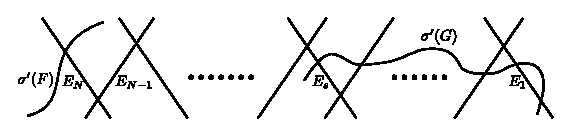
\includegraphics[scale=1.2]{figures/chap2-fig10.eps}

\medskip
{\bf (Fig 1)}
\end{figure}

\noindent
If $g=cg^{\beta_{1}}_{1}\ldots g_{n}^{\beta_{n}}(c\in k^{\ast})$ is a
decomposition of $g$ into $n$ distinct irreducible factors, let
$G_{j}$ be the curve $g_{j}=0$ on $V_{0}:=\mathbb{A}^{2}_{k}$ for
$1\leqq j\leqq n$. Let $\nu_{i}(j)$ be the multiplicity of $G_{j}$ at
the points $P_{i}$ for $1\leqq i\leqq s$ and $1\leqq j\leqq n$. Then
it is clear that
$\nu_{i}=\beta_{1}\nu_{i}(1)+\cdots+\beta_{n}\nu_{i}(n)$ for $1\leqq
i\leqq s$.

\subsection{}\label{chap2:5.5}
We have the following:

\begin{lemma*}
With the same assumption and notations as in \ref{chap2:1.3}, $V$ is
isomorphic, in a neighborhood of $\pi^{-1}(P_{1})$, to $V_{N}$ with
the curves $E_{1},\ldots,E_{N-1}$ and $\sigma'(G)$ deleted off.
\end{lemma*}

\begin{proof}
Let
$\mathscr{O}:=\mathscr{O}_{V_{0},P_{1}},\widetilde{V}_{0}:=\Spec(\mathscr{O})$
and $\widetilde{V}:=\fprod{V}{\widetilde{V}_{0}}{V_{0}}$. Since the
curve $F$ is nonsingular at $P_{1}$ there exist local parameters $u$,
$v$ of $V_{0}$ at $P_{1}$ such that $v=f$. Let $g(u,v)=0$ be a local
equation of $G$ at $P_{1}$. Then
$\widetilde{V}=\Spec(\mathscr{O}[v/g(u,v)])$. Note that $V$ is
nonsingular in a neighborhood of $\pi^{-1}(P_{1})$ (\cf
\ref{chap2:1.2}). Hence there exist a nonsingular projective surface
$\overline{V}$ and a birational mapping $\varphi:V\to \overline{V}$
such that $\varphi$ is an open immersion in a
neighborhood\pageoriginale\ of $\pi^{-1}(P_{1})$ and a birational
mapping
$\overline{\pi}:=\pi\cdot\varphi^{-1}:\overline{V}\to\mathbb{P}^{2}_{k}$
is a morphism, where $V_{0}$ is embedded into the projective plane
$\mathbb{P}^{2}_{k}$ as a complement of a line. Since
$\pi(\pi^{-1}(P_{1}))=P_{1}$ we know that $\overline{\pi}$ is factored
by the quadratic transformation of $\mathbb{P}^{2}_{k}$ with center at
$P_{1}$. Hence we know that $\pi:V\to V_{0}$ is factored by
$\sigma_{1}:V_{1}\to V_{0}$, \iec
$\pi:V\xrightarrow{\pi_{1}}V_{1}\xrightarrow{\sigma_{1}}V_{0}$. 


Set $v=uv_{1}$, $u=vu_{1}$, $q(u,uv_{1})=u^{\nu_{1}}g_{1}(u,v_{1})$
and $g(vu_{1},v)=v^{\nu_{1}}g'_{1}(u_{1},v)$. Then
$\fprod{V_{1}}{\widetilde{V}_{0}}{V_{0}}=\Spec(\mathscr{O}[v_{1}])\cup
\Spec(\mathscr{O}[u_{1}])$; $\sigma^{-1}_{1}(P_{1})$ and
$\sigma'_{1}(G)$ are respectively defined by $u=0$ and
$g_{1}(u,v_{1})=0$ on $\Spec$ $(\mathscr{O}[v_{1}])$, and by $v=0$ and
$g'_{1}(u_{1},v)=0$ on $\Spec(\mathscr{O}[u_{1}])$. Since 
\begin{align*}
\widetilde{V} &:=
\fprod{V}{\widetilde{V}_{0}}{V_{0}}=\fprod{\fprod{V}{(V_{1}}{V_{1}}}{\widetilde{V}_{0})}{V_{0}}=\fprod{V}{\Spec(\mathscr{O}[v_{1}])}{V_{1}}\cup
\fprod{V}{\Spec(\mathscr{O}[u_{1}])}{V_{1}}\\
&=\Spec(\mathscr{O}[v_{1},v_{1}/u^{\nu_{1}-1}g_{1}(u,v_{1})])\cup
\Spec(\mathscr{O}[u_{1},1/v^{\nu_{1}-1}g'_{1}(u_{1},v)]) 
\end{align*}
and since $v$ is an invertible function on $\Spec(\mathscr{O}[u_{1},
  1/v^{\nu_{1}-1}g'_{1}(u_{1},v)])$, we know that:
\begin{enumerate}
\renewcommand{\labelenumi}{(\theenumi)}
\item
  $\widetilde{V}=\Spec(\mathscr{O}[v_{1},v_{1}/u^{\nu_{1}-1}g_{1}(u,v_{1})])$; 

\item
  $\widetilde{\pi}:=\fprod{\pi}{\widetilde{V}_{0}}{V_{0}}:\widetilde{V}\to
  \widetilde{V}_{0}$ is a composition of
  $\widetilde{\pi}_{1}:=\fprod{\pi_{1}}{\widetilde{V}_{0}}{V_{0}}:\widetilde{V}\to
  \widetilde{V}_{1}:=\Spec(\mathscr{O}[v_{1}])$ and
  $\widetilde{\sigma}_{1}:=\sigma_{1}|_{\widetilde{V}_{1}}:\widetilde{V}_{1}\to
  \widetilde{V}_{0}$; 

\item if $Q\in (\sigma^{-1}_{1}(P_{1})\cup
  \sigma'_{1}(G))-\sigma'_{1}(F)$ then $\widetilde{\pi}^{-1}_{1}(Q)=\phi$.
\end{enumerate}

Set $v_{1}=uv_{2},\ldots,v_{s-1}=uv_{s}$ and
$g_{1}(u,v_{1})=u^{\nu_{2}}g_{2}(u,v_{2}),\ldots,g_{s-1}$ $(u,v_{s-1})=u^{\nu_{s}}
g_{s}(u,v_{s})$. Set 
$\widetilde{V}_{2}:=\Spec(\mathscr{O}[v_{2}]),\ldots,
\widetilde{V}_{s}:= \Spec(\mathscr{O}[v_{s}])$.\pageoriginale\ \break  
Then, by the same argument as above, we know that the following
assertions hold for $2\leqq i\leqq s$:
\begin{itemize}
\item[(1)$'$]
  $\widetilde{V}=\Spec(\mathscr{O}[v_{i},v_{i}/u^{\nu_{1}+\cdots+\nu_{i}-i}g_{i}(u,v_{i})])$; 

\item[(2)$'$] $\widetilde{\pi}:\widetilde{V}\to \widetilde{V}_{0}$ is
  a composition of a morphism $\widetilde{\pi}_{i}:\widetilde{V}\to
  \widetilde{V}_{i}$ and $\widetilde{\sigma}_{1}\cdot
  \widetilde{\sigma}_{2}\cdot\ldots\cdot\widetilde{\sigma}_{i}:\widetilde{V}_{i}\to\widetilde{V}_{0}$,
  where
  $\widetilde{\sigma}_{i}:=\sigma_{i}|_{\widetilde{V}_{i}}:\widetilde{V}_{i}\to
  \widetilde{V}_{i-1}$; moreover,
  $\widetilde{\pi}_{i-1}=\widetilde{\sigma}_{i}\cdot
  \widetilde{\pi}_{i}$;

\item[(3)$'$] if $Q\in(\sigma^{-1}_{i}(P_{i})\cup
  (\sigma_{1}\ldots\sigma_{i})'(G))-(\sigma_{1}\ldots\sigma_{i})'(F)$
  then $\widetilde{\pi}^{-1}_{i}(Q)=\phi$. 
\end{itemize}

When $i=s$, the proper transform $(\sigma_{1}\ldots\sigma_{s})'(G)$ of
$G$ on $V_{s}$ does not meet the proper transform
$(\sigma_{1}\ldots\sigma_{s})'(F)$of $F$ on $\widetilde{V}_{s}$ (\cf
the definition of $s$ in \ref{chap2:5.4}). Therefore, in virtue of $(3)'$
above, we know that $g_{s}(u,v_{s})$ is an invertible function on
$\widetilde{V}$, where $g_{s}(u,v_{s})=0$ is the equation of the
proper transform $(\sigma_{1}\ldots\sigma_{s})'(G)$ of $G$ on
$\widetilde{V}_{s}$. Thus,
$\widetilde{V}=\Spec(\mathscr{O}[v_{s},v_{s}/u^{N-s}])$. 

Furthermore, set $v_{s}=uv_{s+1},\ldots,v_{N-1}=uv_{N}$ and
$\widetilde{V}_{s+1}=\Spec$ $(\mathscr{O}[v_{s+1}]),\ldots,
\widetilde{V}_{N} =\Spec (\mathscr{O}[v_{N}])$. Then
it is easy to see that the following assertions hold for $s+1\leqq
i\leqq N$:
\begin{itemize}
\item[(1)$''$]
  $\widetilde{V}=\Spec(\mathscr{O}[v_{i},v_{i}/u^{N-i}])$;

\item[(2)$''$] $\widetilde{\pi}_{s}:\widetilde{V}\to
  \widetilde{V}_{s}$ is a composition of a morphism
  $\widetilde{\pi}_{i}:\widetilde{V}\to \widetilde{V}_{i}$ and
  $\widetilde{\sigma}_{s+1}\cdot\ldots\cdot\widetilde{\sigma}_{i}:\widetilde{V}_{i}\to
  \widetilde{V}_{s}$, where
  $\widetilde{\sigma}_{i}:=\sigma_{i}|_{\widetilde{V}_{i}}:\widetilde{V}_{i}\to
  \widetilde{V}_{i-1}$ and
  $\widetilde{\pi}_{i-1}=\widetilde{\sigma}_{i}\cdot
  \widetilde{\pi}_{i}$. 
\end{itemize}

Then
$\widetilde{V}\cong\widetilde{V}_{N}=\Spec(\mathscr{O}[v_{N}])$. Hence,
$V$ is isomorphic, in a neighborhood of $\pi^{-1}(P_{1})$, to $V_{N}$
with the curves $E_{1},\ldots,E_{N-1}$ and $\sigma'(G)$ deleted
off. In particular, $\pi^{-1}(P_{1})=\epsilon:=E_{N}-E_{N}\cap
E_{N-1}$.
\end{proof}

\subsection{}\label{chap2:5.6}
Assume\pageoriginale\ that we are given two curves (not necessarily
irreducible) $F$, $G$ on a nonsingular surface $V_{0}$ and a point
$P_{1}\in F\cap G$ at which one of $F$ and $G$, say $F$, is
nonsingular. Let $P_{1},P_{2},\ldots,P_{s}$ be all points of $G$ on
$F$ over $P_{1}$, and let $\nu_{1},\ldots,\nu_{s}$ be the
multiplicities of $G$ at $P_{1},\ldots,P_{s}$, respectively. Let
$N:=\nu_{1}+\cdots+\nu_{s}$. As explained in \ref{chap2:5.4}, define
$\sigma:V_{N}\to V_{0}$ as a composition of quadratic transformations
with centers at $N$ points $P_{1},\ldots,P_{N}$ on $F$, each
$P_{i}(2\leqq i\leqq N)$ being infinitely near to $P_{i-1}$ of order
one. We call $\sigma:V_{N}\to V_{0}$ {\em the standard transformation
  of $V_{0}$ with respect to a triplet $(P_{1},F,G)$.} The
configuration of $\sigma^{-1}(F\cup G)$ in a neighborhood of
$\sigma^{-1}(P_{1})$ is given by the Figure 1 in \ref{chap2:5.4}. With the
notations in the Figure 1, we obtain a new surface $V$ by deleting
$E_{1},\ldots,E_{N-1}$ from $V_{N}$. We then say that $V$ is obtained
from $V_{0}$ by {\em the standard process of the first kind with
  respect to} $(P_{1},F,G)$. On the other hand, note that
$(E^{2}_{i})=-2$ for $1\leqq i\leqq N-1$. Hence we obtain a new normal
surface $V'$ from $V_{N}$ by contracting $E_{1},\ldots,E_{N-1}$ to a
point $Q_{1}$ on $V'$ which is a rational double point (\cf Artin [5;
  Theorem 2.7]). We then say that $V'$ is obtained from
$V_{0}$ by {\em the standard process of the second kind with respect
  to} $(P_{1},F,G)$.

\subsection{}\label{chap2:5.7}
We shall next consider the case where, at a point $P_{1}\in F\cap G$,
the curve $G$ is nonsingular. Indeed, we prove the following:

\begin{lemma*}
With the assumption as above, let $V'$ be the surface obtained from
$V_{0}:=\mathbb{A}^{2}_{k}$ by the standard process of the second kind
with respect to $(P_{1},G,F)$. Then, in a neighborhood of
$\pi^{-1}(P_{1})$, $V$ is\pageoriginale\ isomorphic to $V'$ with the
proper transform of $G$ deleted off. If either $F$ is singular at
$P_{1}$ or $i(F,G;P_{1})\geqq 2$, $V$ has a unique rational double
point on $\pi^{-1}(P_{1})$.
\end{lemma*}

\begin{proof}
Let $P_{1},P_{2},\ldots,P_{r}$ be all points of $F$ on $G$ over
$P_{1}$, and let $\mu_{1}$, $\ldots,\mu_{r}$ be the multiplicities of $F$
at $P_{1},\ldots,P_{r}$, respectively. Let
$M:=\mu_{1}+\cdots+\mu_{r}$. We prove the assertion by induction on
$M$. Note that $M=1$ if and only if $i(F,G;P_{1})=1$. It is then easy
to see that $V$ is isomorphic, in a neighborhood of $\pi^{-1}(P_{1})$,
to a surface $V'_{1}$ obtained as follows: Let $\sigma_{1}:V_{1}\to
V_{0}$ be the quadratic transformation of $V_{0}:=\mathbb{A}^{2}_{k}$
with center at $P_{1}$, and let $V'_{1}:=V_{1}=\sigma'_{1}(G)$. Now,
assume that $M>1$. Since $G$ is nonsingular at $P_{1}$ there exist
local parameters $u$, $v$ of $V_{0}$ at $P_{1}$ such that $v=g$. Let
$f(u,v)=0$ be a local equation of $F$ at $P_{1}$. Then, $V$ is
isomorphic, in a neighborhood of $\pi^{-1}(P_{1})$, to an affine
hyper surface $vz=f(u,v)$ in the affine $3$-space
$\mathbb{A}^{3}_{k}$. There exists only one singular point
$Q'_{1}:(u,v,z)=(0,0,\alpha)$ of $V$ lying on $\pi^{-1}(P_{1})$, where
$\alpha=\dfrac{\partial f}{\partial v}(0,0)$. Note that if $\alpha\neq
0$ then $A:=k\left[x,y,\dfrac{f}{g}\right]=k \left[x,y, \dfrac{f-\alpha g}{g}\right]$ and
$i(F,G;P_{1})=i(H,G;P_{1})=M$, where $H$ is the curve on
$\mathbb{A}^{2}_{k}$ defined by $f=\alpha g$. Replacing $f$ by
$f-\alpha g$ we may assume, from the outset and without loss of
generality, that $\alpha=0$. Then we have $\mu_{1}\geqq 2$. Let
$\rho_{1}:W_{1}\to \mathbb{A}^{3}_{k}$ be the quadratic transformation
of $\mathbb{A}^{3}_{k}$ with center at the curve
$\pi^{-1}(P_{1}):u=v=0$, let $V'_{1}$ be the proper transform of $V$
on $W_{1}$, and let $\tau_{1}:=\rho_{1}|_{V'_{1}}:V'_{1}\to V$ be the
restriction of $\rho_{1}$ onto $V'_{1}$.

Set $v=uv_{1}$, $u=vu_{1}$ and
$f(u,uv_{1})=u^{\mu_{1}}f_{1}(u,v_{1})$,
$f(vu_{1},v)=v^{\mu_{1}}\widetilde{f}_{1}(u_{1},v)$.\pageoriginale\
Then $V'_{1}$ is given by $v_{1}z=u^{\mu_{1}-1}f_{1}(u,v_{1})$ with
respect to the coordinate system $(u,v_{1},z)$ and by
$z=u^{\mu_{1}-1}\widetilde{f}_{1}(u_{1},v)$ with respect to the
coordinate system $(u_{1},v,z)$. By construction of $V'_{1}$, $V'_{1}$
dominates the surface $V_{1}$ obtained from $V_{0}$ by the quadratic
transformation $\sigma_{1}$ with center at $P_{1}$;
\[
\xymatrix@C=2cm@R=1.2cm{
V'_{1}\ar[d]^{\pi_{1}}\ar[r]^{\tau_{1}} & V\ar[d]^{\pi}\\
V_{1}\ar[r]^{\sigma_{1}} & V_{0}
}
\]
The proper transform $\tau'_{1}(\pi^{-1}(P_{1}))$ of $\pi^{-1}(P_{1})$
on $V'_{1}$ is given by $u=v_{1}=0$; the curve $\tau^{-1}_{1}(Q'_{1})$
is given by $u=z=0$;
$\tau_{1}:V'_{1}-\tau^{-1}_{1}(Q'_{1})\xrightarrow{\sim}V-\{Q'_{1}\}$;
the singular point of $V'_{1}$ is possibly
$Q'_{2}:(u,v_{1},z)=(0,0,0)$.

The morphism $\pi_{1}:V'_{1}\to V_{1}$ is isomorphic at every point of
$\tau^{-1}_{1}(Q'_{1})$ $-\{Q'_{2}\}$. Indeed, if $v_{1}\neq 0$ and
$\infty$, $\pi_{1}$ is given by
$(u,v_{1},z)=(u,v_{1},u^{\mu_{1}-1}$ $f_{1}(u,v_{1})/v_{1})\mapsto
(u,v_{1})$ which is clearly isomorphic; if $v_{1}=\infty$, $\pi_{1}$
is given by $(u_{1},v,v^{\mu_{1}-1}\widetilde{f}_{1}(u_{1},v))\mapsto
(u_{1},v)$ which is isomorphic as well. Under the morphism $\pi_{1}$,
$\tau^{-1}_{1}(Q'_{1})$ corresponds to $\sigma^{-1}_{1}(P_{1})$ and
$\tau'_{1}$ \break $(\pi^{-1}(P_{1}))$ to the point $P_{2}$; moreover
$\pi^{-1}_{1}(P_{2})=\tau'_{1}(\pi^{-1}(P_{1}))$; 
\begin{figure}[H]
\centering
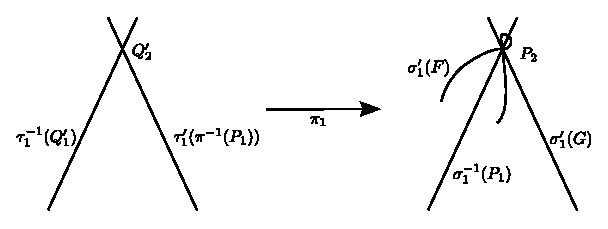
\includegraphics{figures/chap2-fig11.eps}
\end{figure}
Note\pageoriginale\ that the following assertions hold:
\begin{enumerate}
\renewcommand{\labelenumi}{(\theenumi)}
\item $V'_{1}$ is isomorphic, in a neighborhood of
  $\pi^{-1}_{1}(P_{2})$, to an affine hyper surface
  $v_{1}z=u^{\mu_{1}-1}f_{1}(u,v_{1})$ on $\mathbb{A}^{3}_{k}$; 

\item in a neighborhood of $P_{2}$, $\sigma'_{1}(G)$ is defined by
  $v_{1}=0$ and $\sigma'_{1}(F)$ is defined by $f_{1}(u,v_{1})=0$;

\item $P_{2},\ldots,P_{r}$ are all points of the curve
  $F_{1}:u^{\mu_{1}-1}f_{1}(u,v_{1})=0$ on $\sigma'_{1}(G)$ over
  $P_{2}$, and the sum of multiplicities of the curve $F_{1}$ at
  $P_{2},\ldots,P_{r}$ is $M-1$.
\end{enumerate}

Let $V''_{1}$ be the surface obtained from $V'_{1}$ by the standard
process of the second kind with respect to a triplet
$(P_{2},\sigma'_{1}(G),F_{1})$. Then, by the assumption of induction
applied to $V'_{1}$, we know that, in a neighborhood of
$\tau'_{1}(\pi^{-1}(P_{1}))=\pi^{-1}_{1}(P_{2})$, $V'_{1}$ is
isomorphic to $V''_{1}$ with the proper transform of $\sigma'_{1}(G)$
on $V''_{1}$ deleted off. Let $\rho:V_{M}\to V_{1}$ be the standard
transformation of $V_{1}$ with respect to a triplet
$(P_{2},\sigma'_{1}(G),F_{1})$. Then $\sigma_{1}\cdot\rho$ is
clearly the standard transformation $\sigma:V_{M}\to V_{0}$ with
respect to a triplet $(P_{1},G,F)$; 
\begin{figure}[H]
\centering
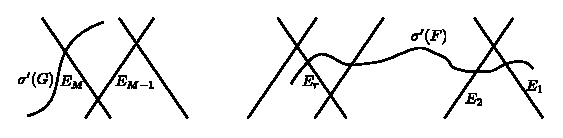
\includegraphics[scale=1.2]{figures/chap2-fig12.eps}

\medskip
{\bf (Fig 2)}
\end{figure}
\noindent
where, in the Figure 2, we have:
\begin{itemize}
\item[$1^{\circ}$] $E_{1}=\rho'(\sigma^{-1}_{1}(P_{1}))$;

\item[$2^{\circ}$] the surface $V'_{1}$ is obtained by contracting
  $E_{2},\ldots,E_{M-1}$ to a point $Q'_{2}$ and by deleting the
  proper transform of $\sigma'(G)$; under\pageoriginale\ this
  contraction, say $\varphi$, we have
  $\varphi(E_{1})=\tau^{-1}_{1}(Q'_{1})$ and $\varphi(E_{M}-E_{M}\cap
  \sigma'(G))=\tau'_{1}(\pi^{-1}(P_{1}))$. 
\end{itemize}

It is now easy to see that $V$ is isomorphic, in a neighborhood of
$\pi^{-1}(P_{1})$, to the surface $V'$ with the proper transform of
$G$ deleted off, where $V'$ is obtained from $V_{M}$ by contracting
$E_{1},\ldots,E_{M-1}$. Hence, the unique singular point of $V$ lying
on $\pi^{-1}(P_{1})$ is a rational double point.
\end{proof}

\subsection{}\label{chap2:5.8}

Let $P_{1}\in F\cap G$, and assume that $G$ is nonsingular at
$P_{1}$. Let $P_{1},P_{2},\ldots$, $P_{r}$ be all points of $F$ on $G$
over $P_{1}$, and let $\mu_{1},\mu_{2},\ldots,\mu_{r}$ be the
multiplicities of $F$ at $P_{1},P_{2},\ldots,P_{r}$, respectively. If
$f=\cf^{\alpha_{1}}_{1}\ldots f^{\alpha_{m}}_{m}(c\in k^{\ast})$ is a
decomposition of $f$ into distinct irreducible factors, let
$F_{j}(1\leq j\leq m)$ be the curve on $V_{0}$ defined by
$f_{j}=0$. Let $\mu_{i}(j)$ be the multiplicity of $F_{j}$ at $P_{i}$
for $1\leqq i\leqq r$ and $1\leqq j\leqq m$. Then it is clear that
$\mu_{i}=\alpha_{1}\mu_{i}(1)+\cdots+\alpha_{m}\mu_{i}(m)$ for $1\leqq
i\leqq r$.

\subsection{}\label{chap2:5.9}

As a consequence of Lemmas \ref{chap2:5.5} and \ref{chap2:5.7}, we have the
following: 

\begin{theorem*}
Assume that $V$ has only isolated singularities. Let $W$ be the
surface obtained from $V_{0}:=\mathbb{A}^{2}_{k}$ by the standard
processes of the first (or the second) kind at every point of $F\cap
G$. Then $V$ is isomorphic to the surface $W$ with the proper
transform of $G$ on $W$ deleted off. The surface $V$ is, therefore, a
normal surface whose singular points (if any) are rational double
points.
\end{theorem*}

\subsection{}\label{chap2:5.10}
In the paragraphs \ref{chap2:5.10} $\sim$ \ref{chap2:5.12} we shall study the
divisor class group $C\ell(V)$. Let $g=cg^{\beta_{1}}_{1}\ldots
g^{\beta_{n}}_{n}(c\in k^{\ast})$ be a decomposition of
$g$\pageoriginale\ into distinct irreducible factors, and let $G_{j}$
be the curve $g_{j}=0$ on $V_{0}$ for $1\leqq j\leqq n$. Assume that
$F\cap G\neq \phi$. Let $F\cap G=\{P_{1}^{(1)},\ldots,p_{1}^{(e)}\}$. For
$1\leqq \ell \leqq e$, either $F$ is nonsingular at $P^{(\ell)}_{1}$
but $G$ is singular, or $G$ is nonsingular at $P_{1}^{(\ell)}$. We may
assume that $F$ is nonsingular at $P^{(1)}_{1},\ldots,P_{1}^{(a)}$ but
$G$ is singular, and $G$ is nonsingular at
$P_{1}^{(a+1)},\ldots,P_{1}^{(e)}$. (The number a may be $0$). For
$1\leqq \ell\leqq a$, let
$P_{1}^{(\ell)},\ldots,P^{(\ell)}_{s_{\ell}}$ be all points of $G$ on
$F$ over $P^{(\ell)}_{1}$, and let $\nu^{(\ell)}_{i}(j)$ be the
multiplicity of $G_{j}$ at $P^{(\ell)}_{i}$ for $1\leqq i\leqq
s_{\ell}$ and $1\leqq j\leqq n$; let
$N^{(\ell)}(j)=\nu^{(\ell)}_{1}(j)+\cdots+\nu^{(\ell)}_{s_{\ell}}(j)$,
let
$\nu^{(\ell)}_{i}=\beta_{1}\nu_{i}^{(\ell)}(1)+\cdots+\beta_{n}\nu_{i}^{(\ell)}(n)$
and let
$N^{(\ell)}=\beta_{1}N^{(\ell)}(1)+\cdots+\beta_{n}N^{(\ell)}(n)$. For
  $a+1\leqq \ell\leqq e$, let
  $P_{1}^{(\ell)},\ldots,P^{(\ell)}_{r_{\ell}}$ be all points of $F$
  on $G$ over $P^{(\ell)}_{1}$, and let $\mu^{(\ell)}_{i}$ be the
  multiplicity of $F$ at $P^{(\ell)}_{i}$ for $1\leqq i\leqq
  r_{\ell}$. Let
  $M^{(\ell)}=\mu^{(\ell)}_{1}+\cdots+\mu^{(\ell)}_{r_{\ell}}$. Since
  $G$ is nonsingular at $P^{(\ell)}_{1}$ for $a+1\leqq \ell\leqq e$,
  there exists a unique $G_{j}(1\leqq j\leqq n)$ such that
  $P^{(\ell)}_{1},\ldots,P^{(\ell)}_{r_{\ell}}$ lie on $G_{j}$. Then
  We set $M^{(\ell)}(j)=M^{(\ell)}$ and $M^{(\ell)}(j')=0$ for $j'\neq
  j$. Let $\epsilon^{(\ell)}:=\pi^{-1}(P^{(\ell)}_{1})$ for $1\leqq
  \ell \leqq e$.

\subsection{}\label{chap2:5.11}

The structure of the divisor class group $C\ell(V)$ is given by the
following:

\begin{theorem*}
With the notations as above, the divisor class group $C\ell(V)$ is
isomorphic to:
$$
\{\mathbb{Z}\epsilon^{(1)}+\cdots+\mathbb{Z}\epsilon^{(e)}\}/\{\sum^{a}_{\ell=1}N^{(\ell)}(j)\epsilon^{(\ell)}+\sum^{e}_{\ell=a+1}M^{(\ell)}(j)\epsilon^{(\ell)};1\leqq
j\leqq n\}.
$$
\end{theorem*}

\begin{proof}
Embed\pageoriginale\ $V_{0}:=\mathbb{A}^{2}_{k}$ into the projective
plane $\mathbb{P}^{2}_{k}$ as a complement of a line
$\ell_{\infty}$. For $1\leqq \ell \leqq e$, let
$E^{(\ell)}_{1},\ldots,E^{(\ell)}_{q}$ be all exceptional curves which
arise from the standard transformation of $V_{0}$ with respect to a
triplet $(P^{(\ell)}_{1},F,G)$ (or $(P^{(\ell)}_{1},G,F)$), where
$q=N^{(\ell)}$ (or $M^{(\ell)}$). Let $\tau:W\to \mathbb{P}^{2}_{k}$
be the composition of standard transformations of $\mathbb{P}^{2}_{k}$
with respect to triplets $(P^{(\ell)}_{1},F,G)$ for $1\leqq \ell\leqq
a$ and triplets $(P^{(\ell)}_{1},G,F)$ for $a+1\leqq \ell\leqq
e$. Then it is easy to see that the divisor
$$
(g_{j})_{W}-\left\{\sum^{a}_{\ell=1}N^{(\ell)}(j)E^{(\ell)}_{N^{(\ell)}}+\sum^{e}_{\ell=a+1}M^{(\ell)}(j)E^{(\ell)}_{M^{(\ell)}}\right\}\quad
(1\leqq j\leqq n) 
$$
has support on $\tau'(G_{j})$, $\tau'(\ell_{\infty})$,
$E^{(\ell)}_{1},\ldots,E^{(\ell)}_{q-1}$ ($q=N^{(\ell)}$ or
$M^{(\ell)}$) for $1\leqq \ell\leqq e$. Hence we have:
$$
(g_{j})_{V}=\sum^{a}_{\ell=1}N^{(\ell)}(j)\epsilon^{(\ell)}+\sum^{e}_{\ell=a+1}M^{(\ell)}(j)\epsilon^{(\ell)}\sim
0 
$$
as a divisor on $V$ for $1\leqq j\leqq n$.

Now, let $C$ be an irreducible curve on $V$ such that $\pi(C)$ is not
a point, and let the closure of $\pi(C)$ on $V_{0}$ be defined by
$h=0$ with $h\in k[x,y]$. Then, by considering the divisor $(h)_{W}$
on $W$, we easily see that $C$ is linearly equivalent to an integral
combination of $\epsilon^{(1)},\ldots,\epsilon^{(e)}$. Hence, by
setting
$$
\mathfrak{g}:=\{\mathbb{Z}\overline{\epsilon}^{(1)}+\cdots+\mathbb{Z}\overline{\epsilon}^{(e)}\}/\left\{\sum^{a}_{\ell=1}N^{(\ell)}(j)\overline{\epsilon}^{(\ell)}+\sum^{e}_{\ell=a+1}M^{(\ell)}(j)\overline{\epsilon}^{(\ell)};1\leqq
j\leqq n\right\}
$$
we have a surjective homomorphism:
$$
\theta:\mathfrak{g}\to C\ell(V);
\theta(\overline{\epsilon}^{(\ell)})=\epsilon^{(\ell)}(1\leqq
\ell\leqq e). 
$$

We shall show that $\theta$ is an isomorphism. Assume that $\Ker
\theta \neq (0)$,\pageoriginale\ and let
$d_{1}\overline{\epsilon}^{(1)}+\cdots+d_{e}\overline{\epsilon}^{(e)}$
be a nonzero element of $\Ker \theta$. Then
$d_{1}\epsilon^{(1)}+\cdots+d_{e}\epsilon^{(e)}=(t)_{V}$ on $V$, where
$t\in k(V)$ such that $t\not\in k$. Then we may write
$(t)_{V_{0}}={\displaystyle{\mathop{\sum}_{i}}}m_{i}C_{i}$ with
irreducible curves $C_{i}$ on $V_{0}$ and nonzero integers
$m_{i}$. Let $t_{i}\in k[x,y]$ be such that $C_{i}$ is defined by
$t_{i}=0$, and write:
$$
(t_{i})_{V}=\pi'(C_{i})+\sum^{e}_{\ell=1}b_{i\ell}\epsilon^{(\ell)}\quad\text{with}\quad
b_{i\ell}\in \mathbb{Z}.
$$
Then, since $t=C{\displaystyle{\mathop{\Pi}_{i}}}t^{m_{i}}_{i}$ with
  $c\in k^{\ast}$ we have:
$$
(t)_{V}=\sum_{i}\{m_{i}\pi'(C_{i})+\sum^{e}_{\ell=1}m_{i}b_{i\ell}\epsilon^{(\ell)}\}=\sum^{e}_{\ell=1}d_{\ell}\epsilon^{(\ell)}.
$$
Hence we know that $\pi'(C_{i})=\phi$ for every $i$. This implies that
every $C_{i}$ must coincide with one of $G_{j}$'s $(1\leqq j\leqq n)$,
\iec $(t)_{V}$ is an integral combination of $(g_{j})_{V}$'s. Hence
$d_{1}\overline{\epsilon}^{(1)}+\cdots+d_{e}\overline{\epsilon}^{(e)}=0$
in $\mathfrak{g}$. This is a contradiction.
\end{proof}

\subsection{}\label{chap2:5.12}
The affine $k$-domain $A=k[x,y,\dfrac{f}{g}]$ is a unique
factorization domain if and only if $C\ell(V)=(0)$. We have the
following two consequences of \ref{chap2:5.11}.

\subsubsection{}\label{chap2:5.12.1}
\begin{coro*}
  With the notations of \ref{chap2:5.10}, if $e>n$ then $A$ is not a unique
  factorization domain.
\end{coro*}

\subsubsection{}\label{chap2:5.12.2}
\begin{coro*}
  Assume that $g$ is irreducible and that $F\cap G\neq \phi$. Then $A$
  is a unique factorization domain if and only if the curves $F$ and $G$
  meet each other in only one point where they intersect transversely.
\end{coro*}

\subsection{}\label{chap2:5.13}
Let\pageoriginale\ $A^{\ast}$ be the group of all invertible elements
of $A=k\left[x,y,\dfrac{f}{g}\right]$. Then $A^{\ast}$ contains $k^{\ast}=k-(0)$
as a subgroup. By virtue of Miyanishi [32; Remark 2, p.174] we know
that $A^{\ast}/k^{\ast}$ is a free $\mathbb{Z}$-module of finite rank
and $A^{\ast}$ is isomorphic to a direct product of $k^{\ast}$ and
$A^{\ast}/k^{\ast}$. The purpose of the present and the next
paragraphs is to determine the group $A^{\ast}/k^{\ast}$. Let $H$ be
the subgroup of
$\mathbb{Z}\epsilon^{(1)}+\cdots+\mathbb{Z}\epsilon^{(e)}$ generated
by
$$
\left\{\sum^{a}_{\ell=1}N^{(\ell)}(j)\epsilon^{(\ell)}+\sum^{e}_{\ell=a+1}M^{(\ell)}(j)\epsilon^{(\ell)};1\leqq
j\leqq n\right\}. 
$$
Let $T_{1},\ldots,T_{n}$ be $n$-indeterminates, and let
$\eta:\mathbb{Z}^{(n)}:=\mathbb{Z}T_{1}+\cdots+\mathbb{Z}T_{n}\to H$
be a homomorphism such that, for $1\leqq i\leqq n$,
$$
\eta(T_{i})=\sum^{a}_{\ell=1}N^{(\ell)}(j)\epsilon^{(\ell)}+\sum^{e}_{\ell=a+1}M^{(\ell)}(j)\epsilon^{(\ell)}.
$$
Let $L$ be the kernel of $\eta$, and define a homomorphism $\xi:L\to
K^{\ast}$ (where $K=k(x,y)$) by
$$
\xi(\gamma_{1}T_{1}+\cdots+\gamma_{n}T_{n})=g^{\gamma_{1}}_{1}\ldots
g^{\gamma_{n}}_{n},\quad\text{where}\quad \gamma_{i}\in\mathbb{Z}.
$$
Then we have the following:

\begin{lemma*}
The homomorphism $\xi$ induces an isomorphism $\overline{\xi}:L\xrightarrow{\sim}A^{\ast}/k^{\ast}$.
\end{lemma*}

\begin{proof}
\begin{enumerate}
\renewcommand{\labelenumi}{(\theenumi)}
\item Since
  $(g_{i})_{V}={\displaystyle{\mathop{\sum}_{\ell=1}^{a}}}N^{(\ell)}(j)\epsilon^{(\ell)}+{\displaystyle{\mathop{\sum}_{\ell=a+1}^{e}}}M^{(\ell)}(j)\epsilon^{(\ell)}=\eta(T_{i})$
  for $1\leqq i\leqq n$, we have:
$$
\eta(\gamma_{1}T_{1}+\cdots+\gamma_{n}T_{n})=(g^{\gamma_{1}}_{1}\ldots g^{\gamma_{n}}_{n})_{V}.
$$
Therefore, if $\gamma_{1}T_{1}+\cdots+\gamma_{n}T_{n}\in L$ then
$g^{\gamma_{1}}_{1}\ldots g^{\gamma_{n}}_{n}$ is an invertible
element\pageoriginale\ of $A$, which is a constant if and only if
$\gamma_{1}=\ldots=\gamma_{n}=0$. Thus, $\xi$ induces a monomorphism
$\overline{\xi}$ from $L$ into $A^{\ast}/k^{\ast}$. 

\item Let $t$ be a non-constant invertible element of $A$. Write
  $(t)_{V_{0}}={\displaystyle{\mathop{\sum}_{i}}}m_{i}C_{i}$ with
  irreducible curves $C_{i}$ and nonzero integers $m_{i}$. Let $C_{i}$
  be defined by $t_{i}=0$ with $t_{i}\in k[x,y]$. As in the proof of
  \ref{chap2:5.11}, write: 
$$
(t_{i})_{V}=\pi'(C_{i})+\sum^{e}_{\ell=1}b_{i\ell}\epsilon^{(\ell)}\quad\text{with}\quad
  b_{i\ell}\in \mathbb{Z}. 
$$
Then we have:
$$
(t)_{V}=\sum_{i}\left\{m_{i}\pi'(C_{i})+\sum^{e}_{\ell=1}m_{i}b_{i\ell}\epsilon^{(\ell)}\right\}=0.
$$
Hence we have $\pi'(C_{i})=\phi$ for every $i$. This implies that
$C_{i}$ must coincide with one of $G_{j}$'s. Hence we could write:
$$
(t)_{V_{0}}=\sum^{n}_{j=1}m_{j}G_{j}
$$
where $m_{j}$ may be zero. Then $t=cg^{m_{1}}_{1}\ldots g^{m_{n}}_{n}$
with $c\in k^{\ast}$. It is then clear that
$m_{1}T_{1}+\cdots+m_{n}T_{n}\in L$ and
$\xi(m_{1}T_{1}+\cdots+m_{n}T_{n})=t/c$. Therefore,
$\overline{\xi}:L\to A^{\ast}/k^{\ast}$ is an isomorphism.
\end{enumerate}
\end{proof}

\subsection{}\label{chap2:5.14}
By virtue of \ref{chap2:5.11} and \ref{chap2:5.13}, we have the following:

\begin{theorem*}
Assume that $V$ has only isolated singularities. Then we have the
following exact sequence of $\mathbb{Z}$-modules:
$$
0\to A^{\ast}/k^{\ast}\to \mathbb{Z}^{(n)}\to\mathbb{Z}^{(e)}\to
C\ell(V)\to 0,
$$
where $\mathbb{Z}^{(r)}$ stands for a free $\mathbb{Z}$-module of rank
$r$; $n$ is the number of\pageoriginale\ distinct irreducible factors
of $g$; $e$ is the number of distinct points of $F\cap G$.
\end{theorem*}

\subsection{}\label{chap2:5.15}
\begin{remarks*}
  \begin{enumerate}
    \renewcommand{\labelenumi}{(\theenumi)}
  \item It is clear from \ref{chap2:5.14} that if $g$ is irreducible then
    $A^{\ast}=k^{\ast}$. 
    
  \item $\rank(C\ell(V))-\rank(A^{\ast}/k^{\ast})=e-n$.
    
  \item Though we proved Theorem \ref{chap2:5.14} under the assumption that
    $F\cap G\neq \phi$ it is clear that the theorem is valid also in the
    case $F\cap G=\phi$.
  \end{enumerate}
\end{remarks*}

\subsection{}\label{chap2:5.16}
From now on in the remaining paragraphs of this section we assume that
the characteristic of $k$ is zero. Assume that
$A:=k[x,y,\dfrac{f}{g}]$ is normal and $A$ has a nontrivial locally
nilpotent $k$-derivation $D$ (\cf (\ref{chap1:1.1})). By virtue of
\ref{chap1:1.2} we know that $D$ defines a nontrivial action of the
additive group scheme $G_{a,k}$ on $V$ and {\em vice versa}. Then we
have the following:

\begin{lemma*}[\cf \ref{chap1:1.3.1}, \ref{chap1:1.6} ]
The subring $A_{0}$ of $D$-constants is a finitely generated, normal,
rational $k$-domain of dimension $1$.
\end{lemma*}

\begin{proof}
The fact that $A_{0}$ is rational over $k$ follows from L\"uroth's theorem.
\end{proof}

\subsection{}\label{chap2:5.17}
By virtue of the previous lemma we may write
$A_{0}=k\left[t,\dfrac{1}{h(t)}\right]$ with $h(t)\in k[t]$; $U:=\Spec(A_{0})$ is
an open set of the affine line $\mathbb{A}^{1}_{k}$. Let $q:V\to U$ be
the morphism defined by the canonical inclusion $A_{0}\hookrightarrow
A$. For almost all elements $\alpha$ of $k$ such that $h(\alpha)\neq
0$, the fiber $q^{-1}(\alpha)$ is a $G_{a}$-orbit with respect to the
$G_{a}$-action on $V$ corresponding to $D$, and hence $q^{-1}(\alpha)$
is isomorphic\pageoriginale\ to the affine line
$\mathbb{A}^{1}_{k}$. Let $\rho:V'\to V$ be the minimal resolution of
singularities of $V$\footnote{For the existence of the minimal
  resolution of singularities of $V$, we refer to Lipman [30; Th.\@ 4.1].}. As we saw in \ref{chap2:5.9}, singular points
of $V$ are rational double points. Hence, $\rho$ is a composition of
quadratic transformations with centers at singular points. Let
$q':=q\cdot\rho:V'\to U$. Almost all fibers of $q'$ are therefore
isomorphic to the affine line $\mathbb{A}^{1}_{k}$. Now we shall prove
the following:

\begin{lemma*}
There exists a nonsingular projective surface $W$ and a surjective
morphism $p$\footnote{Since $k$ is assumed to be of characteristic
  zero there would not be a confusion of notations.}:$W\to
\mathbb{P}^{1}_{k}$ satisfying the following conditions:
\begin{enumerate}
\renewcommand{\labelenumi}{\rm(\theenumi)}
\item Almost all fibers of $p$ are isomorphic to $\mathbb{P}^{1}_{k}$.

\item There exists an open immersion $l:V'\to W$ such that $p\cdot
  l=\overline{l}\cdot q'$, where $\overline{l}:U\hookrightarrow
  \mathbb{P}^{1}_{k}$ is the canonical open immersion via
  $U\hookrightarrow \mathbb{A}^{1}_{k}:=\Spec(k[t])$.

\item The fibration $p$ has a cross-section $S$ such that $S\subset
  W-l(V')$. 
\end{enumerate}
\end{lemma*}

\begin{proof}
Let $\overline{V}$ be a nonsingular projective surface containing $V'$
as an open set. Then, a sub field $k(t)$ of $k(V')=k(\overline{V})$
defines a linear pencil $\overline{\Lambda}$ of effective divisors on
$\overline{V}$ such that a general member of $\overline{\Lambda}$ cuts
out a general fiber of $q'$ on $V'$. The base points of
$\overline{\Lambda}$ are situated on $\overline{V}-V'$. Let
$\theta:W\to \overline{V}$ be the shortest succession of quadratic
transformations of $\overline{V}$ with centers at the base points of
$\overline{\Lambda}$ such that the proper transform $\Lambda$
of\pageoriginale\ $\overline{\Lambda}$ by $\theta$ has no base points,
and let $p:W\to \mathbb{P}^{1}_{k}$ be the morphism defined by
$\Lambda$. Since $V'$ is naturally embedded into $W$ as an open set,
let $l:V'\to W$ be the natural open immersion. Then it is not hard to
see that $p:W\to\mathbb{P}^{1}_{k}$ and $l:V'\to W$ satisfy the
conditions (1), (2) and (3) of Lemma.
\end{proof}

\subsection{}\label{chap2:5.18}
Lemma \ref{chap2:2.2} applied to the fibration $p:W\to
\mathbb{P}^{1}_{k}$ implies the following:

\begin{lemma*}
  Write $W-l(V')={\displaystyle{\mathop{\bigcup}^{r}_{i=1}}}C_{i}$ with
  irreducible curves $C_{i}$. Then we have:
  \begin{enumerate}
    \renewcommand{\labelenumi}{\rm(\theenumi)}
  \item Every $C_{i}$ is isomorphic to $\mathbb{P}^{1}_{k}$.
    
  \item For $i\neq j$, $C_{i}$ and $C_{j}$ meet each other (if at all)
    in a single point where they intersect transversely.
    
  \item For three distinct indices $i$, $j$ and $\ell$, $C_{i}\cap
    C_{j}\cap C_{\ell}=\phi$.
    
  \item ${\displaystyle{\mathop{\bigcup}^{r}_{i=1}}}C_{i}$ does not
    contain any cyclic chains.
  \end{enumerate}
\end{lemma*}

\begin{proof}
Note that one of $C_{i}$'s is the cross-section $S$ and the other
components are contained in the fibers of $p$. Noting that $S$ is
isomorphic to $\mathbb{P}^{1}_{k}$, we obtain readily the above
assertions from Lemma \ref{chap2:2.2}.
\end{proof}

\subsection{}\label{chap2:5.19}
Let $V_{0}:=\Spec(k[x,y])$, and let $F$, $G$ be as in \ref{chap2:5.2}. Let
$G_{j}(1\leq j\leq n)$ be as in \ref{chap2:5.10}. Embed $V_{0}$ into the
projective plane $\mathbb{P}^{2}_{k}$ as the complement of a line
$\ell_{\infty}$, and let $\overline{F}$, $\overline{G}$,
$\overline{G}_{j}(1\leqq j\leqq n)$ be the closures of $F$, $G$,
$G_{j}$ in $\mathbb{P}^{2}_{k}$, respectively. Let $\tau:Z\to
\mathbb{P}^{2}_{k}$ be a composition of the standard transformations
of $\mathbb{P}^{2}_{k}$ with respect to triplets $(P,F,G)$ (or
$(P,G,F)$), where $P$ runs over all points\pageoriginale\ of $F\cap
G$. Then we know that $V'$ is embedded into $Z$ as an open set. We may
assume, by replacing $W$ if necessary by a surface which is obtained
from $W$ by a succession of the quadratic transformations, that there
exists a birational morphism $\varphi:W\to Z$ such that we have the
following commutative diagram:
\[
\xymatrix@C=1.7cm@R=1.2cm{
 & W\ar[dl]_{\varphi}\ar[r]^{p} & \mathbb{P}^{1}_{k}\\
Z\ar[dd]^{\tau} & V'\ar@{_{(}->}[l]\ar[r]^{q'}\ar[d]^{\rho}
  \ar@{^{(}->}[u]_{l} & U\ar@{^{(}->}[u]_{\overline{l}}\\
 & V\ar[d]^{\pi} &\\
\mathbb{P}^{2}_{k} & V_{0}\ar@{_{(}->}[l] &
}
\]

\subsection{}\label{chap2:5.20}
\begin{lemma*}
\begin{enumerate}
\renewcommand{\labelenumi}{\rm(\theenumi)}
\item With the notations of \ref{chap2:5.19},
  $(\tau\varphi)'(\overline{G}_{j})$ is contained in a fiber of $p$
  for $1\leqq j\leqq n$; in particular,
  $(\tau\varphi)'(\overline{G}_{j})$ is isomorphic to
  $\mathbb{P}^{1}_{k}$.

\item Let $P_{1}\in F\cap G$. Assume that $F$ is nonsingular at
  $P_{1}$ but $G$ is singular at $P_{1}$. Then, with the notations of
  the Figure $1$ of \ref{chap2:5.4},
  $\varphi'(E_{1}),\ldots,\varphi'(E_{N-1})$ are contained in one and
  only one fiber of $p$.
\end{enumerate}
\end{lemma*}

\begin{proof}
\begin{enumerate}
\renewcommand{\labelenumi}{(\theenumi)}
\item We know by virtue of \ref{chap2:5.17} that if $\lambda$ is a general
  member of $p$ then $\lambda_{V'}:=l^{-1}(\lambda\cap l(V'))$ is
  isomorphic to the affine line $\mathbb{A}^{1}_{k}$; we also know
  that $\pi'(G_{j})=\phi$ for $1\leqq j\leqq n$. Hence
  $\lambda_{V'}\cap (\pi\rho)'(G_{j})=\phi$. This implies that if
  $(\tau\varphi)'(\overline{G}_{j})\cap \lambda\neq\phi$ then
  $\lambda$ meets $(\tau\varphi)'(\overline{G}_{j})$ at some of
  finitely many points of $(\tau\varphi)'(\overline{G}_{j})$
  which\pageoriginale\ are independent of choice of $\lambda$. However,
  this is impossible because $\lambda$ is a general member of an
  irreducible linear pencil on $W$ free from base points. Hence
  $(\tau\varphi)'(\overline{G}_{j})\cap\lambda=\phi$. This implies
  that $(\tau\varphi)'(\overline{G}_{j})$ is contained in a fiber of
  $p$ for $1\leqq j\leqq n$. The fact that
  $(\tau\varphi)'(\overline{G}_{j})$ is isomorphic to
  $\mathbb{P}^{1}_{k}$ follows from Lemma \ref{chap2:2.2}.

\item By construction of $V$ and $V'$ (\cf \ref{chap2:5.9}) we know that
  $\varphi'(E_{i})\cap l(V')=\phi$ for $1\leqq i\leqq N-1$. Hence, for
  each $i$ with $1\leqq i\leqq N-1$, a general fiber $\lambda$ of $p$
  meets $\varphi'(E_{i})$ at some of finitely many points of
  $\varphi'(E_{i})$ which are independent of choice of $\lambda$. By
  the same reason as in (1) above we know that $\varphi'(E_{i})$ is
  contained in a fiber of $p$. Since
  $\varphi'(E_{1}),\ldots,\varphi'(E_{N-1})$ are connected they are 
contained in one and only one fiber of $p$.
\end{enumerate}
\end{proof}

Note that, with the notations of the assertion (2) above, a general
fiber $\lambda$ of $p$ may intersect $\varphi'(E_{N})$. 

\subsection{}\label{chap2:5.21}
\begin{lemma*}
\begin{enumerate}
\renewcommand{\labelenumi}{\rm(\theenumi)}
\item For $1\leqq j\leqq n$, $G_{j}$ has only one place at infinity;
  every singular point of $G_{j}$ is a one-place point.

\item For distinct $i$, $j~(1\leqq i,j\leqq n)$, $G_{i}\cap G_{j}=\phi$.
\end{enumerate}
\end{lemma*}

\begin{proof}
Let $\Lambda_{Z}$ be the linear pencil on $Z$ defined by a subfield
$k(t)=k(\mathbb{P}^{1})$ of $k(Z)=k(W)$, the inclusion
$k(t)\hookrightarrow k(Z)$ corresponding to $p$. A general member of
$\Lambda_{Z}$ cuts out on $V'$ a curve of the form $\lambda_{V'}$,
where $\lambda$ is a fiber of $p$. Hence, if $\Lambda_{Z}$ has base
points they are centered at a point on $\tau'(\ell_{\infty})$. If
$\varphi$ is not an isomorphism, we may assume without loss of
generality that $\varphi$ is the shortest succession of quadratic
transformations with centers at base points of $\Lambda_{Z}$
(including infinitely near base points) such\pageoriginale\ that the
proper transform of $\Lambda_{Z}$ by $\varphi$ has no base
points. Then every singular point of $G_{j}(1\leqq j\leqq n)$ lies on
the curve $F$; indeed, if otherwise,
$(\tau\varphi)'(\overline{G}_{j})$ has a singular point, which
contradicts Lemma \ref{chap2:5.20}, (1). Now, if $G_{j}$ has two or more
places at infinity then $W-l(V')$ would contain a cyclic chain because
$l(V')\cap
((\tau\varphi)'(\overline{G}_{j})\cup\varphi^{-1}(\tau'(\ell_{\infty})))=\phi$,
which contradicts Lemma \ref{chap2:5.18}. Thus, $G_{j}(l\leqq j\leqq n)$
has only one place at infinity. If $G_{j}$ has a singular point
$P_{1}$ which is not a one-place point, then $P_{1}\in G_{j}\cap F$ as
remarked above and, with the notations of the Figure 1 of \ref{chap2:5.4},
$(\tau\varphi)'(\overline{G}_{j})\cup
\varphi'(E_{1})\cup\ldots\cup\varphi'(E_{N-1})$ would contain a cyclic
chain. Since $(\tau\varphi)'(\overline{G}_{j})$ and
$\varphi'(E_{i})(1\leqq i\leqq N-1)$ are contained in $W-l(V')$ this
is a contradiction to Lemma \ref{chap2:5.18}. Thus, every singular point
of $G_{j}$ is a one-place point. Similarly, if $G_{i}\cap
G_{j}\neq\phi(i\neq j)$ then $W-l(V')$ would contain a cyclic
chain. Thus, $G_{i}\cap G_{j}=\phi$ for $i\neq j$. 
\end{proof}

\subsection{}\label{chap2:5.22}
\begin{lemma*}
  For $1\leqq j\leqq n$, the curve $G_{j}$ is nonsingular.
\end{lemma*}

\begin{proof}
As remarked in the proof of Lemma \ref{chap2:5.21}, if $P$ is a singular
point of $G_{j}$ then $P\in F\cap G_{j}$. Then, in a neighborhood of
$\tau^{-1}(P)$, $\tau^{-1}(F\cup G_{j})$ must have the following
configuration as in the Figure 1 of 5.4:
\begin{figure}[H]
\centering
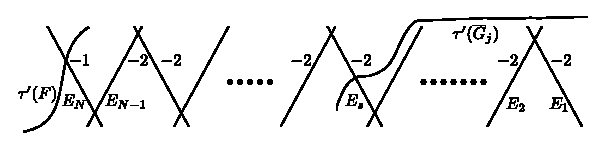
\includegraphics{figures/chap2-fig13.eps}
\end{figure}
\noindent
where\pageoriginale\ $\varphi'(E_{1}),\ldots,\varphi'(E_{N-1})$ and
$(\tau\varphi)'(\overline{G}_{j})$ belong to the same fiber of
$p$. Note that $N\geqq s+1$ since $P$ is a singular point of $G_{j}$
and that $(\tau\varphi)'(\overline{G}_{j})$ intersects
$\varphi'(E_{s})$ transversely in one point. Assume that
$\nu_{b}\geqq 2$ and $\nu_{b+1}=\ldots=\nu_{s}=1$ (\cf \ref{chap2:5.4} for
the notations). Such $b$ exists because $P$ is a singular point of
$G_{j}$ and $(\varphi'(E_{s})\cdot
(\tau\varphi)'(\overline{G}_{j}))=1$. Then it is not hard to show that
$s=b+1$ and we have the configuration:
\begin{figure}[H]
\centering
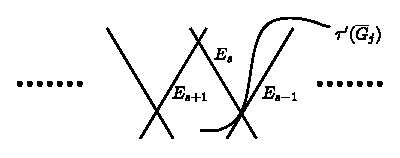
\includegraphics[scale=1.1]{figures/chap2-fig14.eps}
\end{figure}
\noindent
where $\tau'(\overline{G}_{j})$ touches $E_{s-1}$ with
$(\tau'(\overline{G}_{j})\cdot E_{s-1})=\nu_{b}-1\geqq 1$. This
contradicts Lemma \ref{chap2:2.2}. Therefore, the curve $G_{j}$ is
nonsingular. 
\end{proof}

\subsection{}\label{chap2:5.23}
\begin{theorem*}
  Assume that $V$ has only isolated singularities. Then $A$ has a
  nontrivial locally nilpotent $k$-derivation if and only if we have
  $g\in k[y]$ after a suitable change of coordinates $x$, $y$ of $k[x,y]$.
\end{theorem*}

\begin{proof}
Assume that $g\in k[y]$ after a suitable change of coordinates $x$,
$y$ of $k[x,y]$. Then $D=g\dfrac{\partial}{\partial x}$ is a
nontrivial locally nilpotent $k$-derivation on $A$. We shall prove the
converse. With the notations of \ref{chap2:5.16} $\sim$ \ref{chap2:5.22},
$G_{j}(1\leqq j\leqq n)$ is a nonsingular rational curve with only one
place at infinity (\cf \ref{chap2:5.20}, \ref{chap2:5.21} and
\ref{chap2:5.22}).\pageoriginale\ Hence, $G_{j}$ is isomorphic to the affine
line $\mathbb{A}^{1}_{k}$. By virtue of the Embedding theorem of
Abhyankar-Moh (\cf \ref{chap2:1.1}), we may assume that $g_{1}=y$ after a
suitable change of coordinates $x$, $y$ of $k[x,y]$. Then, for $2\leqq
j\leqq n$, $g_{j}$ is written in the form $g_{j}=c_{j}+yh_{j}$ with
$c_{j}\in k$ and $h_{j}\in k[x,y]$ because $G_{j}\cap G_{1}=\phi$ (\cf
\ref{chap2:5.21}, (2)). On the other hand, by virtue of the Irreducibility
theorem (\cf \ref{chap2:1.1}), the fact that $G_{j}$ has only one place at
infinity implies that the curve $g_{j}=\alpha$ on $\mathbb{A}^{2}_{k}$
is irreducible for every $\alpha\in k$. Therefore, $h_{j}$ is a
constant $\in k$. Thus $g\in k[y]$.
\end{proof}

\subsection{}\label{chap2:5.24}
We know by virtue of Theorem \ref{chap2:1.3.1} that $A$ is isomorphic to a
polynomial ring over $k$ if and only if $A$ satisfies the following
conditions:
\begin{enumerate}
\renewcommand{\labelenumi}{(\theenumi)}
\item $A$ is a unique factorization domain,

\item $A^{\ast}=k^{\ast}$,

\item $A$ has a nontrivial locally nilpotent $k$-derivation.
\end{enumerate}
The condition (1) above can be described as follows:

\begin{lemma*}
Assume that $A:=k[x,y,\dfrac{f}{g}]$ satisfies the conditions $(2)$
and $(3)$ above. We may assume that $g\in k[y]$ after a suitable
change of coordinates $x$, $y$ of $k[x,y]$. Write:
$f(x,y)=a_{0}(y)+a_{1}(y)x+\cdots+a_{r}(y)x^{r}$ with $a_{i}(y)\in
k[y]$ $(0\leqq i\leqq r)$. Then $A$ is a unique factorization domain
if and only if $a_{1}(y)$ is a unit modulo $gk[x,y]$ and $a_{i}(y)$ is
nilpotent modulo $gk[x,y]$ for $2\leqq i\leqq r$.
\end{lemma*}

\begin{proof}
Assume that $A$ is a unique factorization domain. With the notations
of \ref{chap2:5.10}, we have $a=0$ because every $G_{j}(1\leqq j\leqq n)$
is\pageoriginale\ nonsingular and $G_{j}\cap G_{i}=\phi$ if $i\neq
j$. By virtue of \ref{chap2:5.14}, we have $e=n$. Theorem \ref{chap2:5.11} then
implies that every $G_{j}$ intersects $F$ transversely. This is
easily seen to be equivalent to the condition on $f(x,y)$ in the above
statement. The ``if'' part of Lemma will be clear by the above
argument and Theorem \ref{chap2:5.11}.
\end{proof}

\subsection{}\label{chap2:5.25}
Finally, we shall prove the following:

\begin{theorem*}[\cf Russell \cite{49} and Sathaye \cite{52} in case
    $m=1$; \cf Wright \cite{56} in case $m>1$]
Let $k$ be an algebraically closed field of characteristic zero and
let $k[x,y]$ be a polynomial ring over $k$ in two variables $x$ and
$y$. Let $f$ and $g$ be two nonzero elements of $k[x,y]$ such that:
\begin{enumerate}
\renewcommand{\labelenumi}{\rm(\theenumi)}
\item $f$ and $g$ have no nonconstant common factors;

\item let $B:=k[x,y,w]/(gw^{m}-f)$ with a variable $w$ and an integer
  $m\geqq 1$; then $B$ is isomorphic to a polynomial ring over
  $k$. Then there exist $\varphi$, $\psi\in k[x,y,w]$ such that
  $k[x,y,w]=k[\varphi,\psi,gw^{m}-f]$. 
\end{enumerate}
\end{theorem*}

\begin{proof}
We shall prove the theorem only in the case where $m>1$; for the case
where $m=1$, see the original proofs. Our proof consists of four
steps.
\begin{enumerate}
\renewcommand{\theenumi}{\Roman{enumi}}
\renewcommand{\labelenumi}{\rm(\theenumi)}
\item Let $A:=k[x,y,z]/(gz-f)$. Let $V:=\Spec(A)$ and
  $W:=\Spec(B)$. By assigning $x$, $y$, $w^{m}$ to $x$, $y$, $z$,
  respectively we have an inclusion $A\hookrightarrow B$, which
  defines in turn a morphism $g:W\to V$. Let $\mathfrak{g}$ be the
  group of $m$-th roots of unity; $\mathfrak{g}$ is identified with a
  cyclic group $\mathbb{Z}_{m}$ of order $m$. Note that $\mathfrak{g}$
  acts on $W$ via $(x,y,w)\mapsto (x,y,\xi w)$ for
  $\xi\in\mathfrak{g}$. It is readily ascertained that $A$ is
  the\pageoriginale\ subring of $\mathfrak{g}$-invariants in $B$ and
  that the morphism $q:W\to V$ is the quotient morphism for the
  above-defined action of $\mathfrak{g}$ on $W$.

\item For the moment, assume only that $W$ is nonsingular. By applying
  the Jacobian criterion of singularity to $W$ we easily see that;
\begin{itemize}
\item[$1^{\circ}$] the curve $F$ on
  $\mathbb{A}^{2}_{k}:=\Spec(k[x,y])$ defined by $f=0$ is a
  nonsingular curve;

\item[$2^{\circ}$] let $G$ be the curve on $\mathbb{A}^{2}_{k}$
  defined by $g=0$; then, if $G$ intersects $F$ at a point $P$, either
  $G$ is singular at $P$ or $G$ intersects $F$ transversely at $P$.
\end{itemize}
This implies by virtue of \ref{chap2:5.3} that if $W$ is nonsingular then
$V$ is nonsingular as well. Let $\pi:V\to \mathbb{A}^{2}_{k}$ be a
morphism defined by $(x,y,z)\mapsto (x,y)$. Note that $(\pi
q)^{-1}(Q)\neq \phi$ and $\pi^{-1}(Q)\neq \phi$ for every point $Q$ on
$F$, and that the proper transform $\pi'(F)$ of $F$ on $V$ is defined
by $z=0$. Moreover, note that the morphism $q:W\to V$ is a finite
morphism, which is unramified at every point $P$ of $V$ with $P\not\in
\pi'(F)$ and totally ramified on the curve $\pi'(F)$.

\item Assume now that $W$ is isomorphic to the affine plane
  $\mathbb{A}^{2}_{k}$. Then $\mathfrak{g}$ is a finite subgroup of
  $\Aut_{k}W$. Since $V$ is nonsingular as seen in the step (II),
  Proposition \ref{chap2:3.7} implies that $V$ is isomorphic to the
  affine plane $\mathbb{A}^{2}_{k}$ as well. We shall show that $F$ is
  isomorphic to the affine line $\mathbb{A}^{1}_{k}$. Write
  $W:=\Spec(k[u,v])$. Since $\mathfrak{g}$ is conjugate to a finite
  subgroup of $GL(2,k)$ (\cf \ref{chap2:3.5}) and since a finite subgroup of
  $GL(2,k)$ isomorphic to $\mathbb{Z}_{m}$ is diagonalizable, we may
  assume that $\mathfrak{g}$ acts on $W$ via
$$
\xi
\begin{pmatrix}
u\\
v
\end{pmatrix}
=
\begin{pmatrix}
\xi^{i} & 0\\
0 & \xi^{j}
\end{pmatrix}
\begin{pmatrix}
u\\
v
\end{pmatrix}
$$\pageoriginale\
where $\xi\in\mathfrak{g}$ and $i$, $j\in\mathbb{Z}_{m}$. Since
$q:W\to V$ is totally ramified over $\pi'(F)$, every point of the
ramification locus of $q$ is fixed by $\mathfrak{g}$. Hence either
$i=0$ or $j=0$. We may assume that $i=0$. Then the curve $R$ on $W$
defined by $v=0$ is the ramification locus of $q$. Since
$\pi'(F)=q(R)$ and $\pi'(F)$ is isomorphic to $R$, we know that
$\pi'(F)$ is isomorphic to the affine line. Therefore, $F$ is an
irreducible nonsingular rational curve with only one place at infinity
(\cf the step (II)). Thus, $F$ is isomorphic to the affine line
$\mathbb{A}^{1}_{k}$. 

\item By virtue of the Embedding theorem (\cf \ref{chap2:1.1}) we may assume
  that $f=x$. On the other hand, since $V$ is isomorphic to the affine
  plane $\mathbb{A}^{2}_{k}$, we know by virtue of Lemma \ref{chap2:5.24}
  and its proof that the curve $G$ is nonsingular, each connected
  component of $G$ is isomorphic to $\mathbb{A}^{1}_{k}$ and $F$
  intersects each connected component of $G$ transversely at a single
  point. Therefore, we may assume that $g\in k[y]$ (\cf
  \ref{chap2:1.3.2}). Then it is easily verified that
  $k[x,y,w]=k[y,z,gw^{m}-f]$.
\end{enumerate}
\end{proof}

\section{Certain affine plane curves with two places at
  infinity}\label{chap2:sec6}\pageoriginale\ 

\subsection{}\label{chap2:6.1}
The results of this section were worked out jointly by T.\@ Sugie and
the lecturer (\cf Miyanishi and Sugie \cite{37}). Throughout the
section the ground field $k$ is assumed to be an algebraically closed
field of characteristic zero. Our ultimate purpose is to prove the
following:

\begin{theorem*}
Let $f$ be an irreducible element of a polynomial ring $k[x,y]$ and
let $C_{\alpha}$ be the curve on $\mathbb{A}^{2}_{k}:=\Spec(k[x,y])$
defined by $f=\alpha$ for $\alpha\in k$. The, after a suitable change
of coordinates $x$, $y$ of $k[x,y]$, $f=c(x^{d}y^{e}-1)$ for $c\in
k^{\ast}$ and positive integers $d$ and $e$ with $(d,e)=1$ if and only
if the following conditions are satisfied:
\begin{enumerate}
\renewcommand{\labelenumi}{\rm(\theenumi)}
\item $f$ is a field generator {\em(\cf \ref{chap2:2.4.1})}.

\item $C_{\alpha}$ has exactly two places at infinity for almost all
  $\alpha\in k$.

\item $C_{\alpha}$ is connected for every $\alpha\in k$.
\end{enumerate}
\end{theorem*}

\subsection{}\label{chap2:6.2}
Let $V$ be a nonsingular projective surface defined over $k$ and let
$\Lambda$ be an irreducible linear pencil on $V$ whose general members
are rational curves. Let $B$ be the set of (ordinary) base points of
$\Lambda$. {\em We assume that each point of $B$ is a one-place point
  of a general member of $\Lambda$.} A reducible member $\Delta$ of
$\Lambda$ is said to be {\em linear} if the following conditions are
satisfied;
\begin{enumerate}
\renewcommand{\theenumi}{\roman{enumi}}
\renewcommand{\labelenumi}{(\theenumi)}
\item every irreducible component of $\Delta$ is isomorphic to
  $\mathbb{P}^{1}_{k}$, 

\item two distinct irreducible components of $\Delta$ meet each other
  (if\pageoriginale\ at all) transversely in a single point,

\item three distinct irreducible components of $\Delta$ have no points
  in common,

\item the weighted graph of $\Delta$ is a linear chain.
\end{enumerate}
An irreducible component $D$ of a linear reducible member $\Delta$ of
$\Lambda$ is called {\em a terminal component} if $D$ meets only one
irreducible component of $\Delta$ other than $D$. An irreducible curve
$S$ on $V$ is called {\em a quasi-section of } $\Lambda$ if $S$ is not
contained in any member of $\Lambda$ and $\Lambda$ has no base points
on $S$; a quasi-section of $\Lambda$ is called {\em a section of}
$\Lambda$ if $(C\cdot S)=1$ for a general member $C$ of $\Lambda$.


\subsection{}\label{chap2:6.3}
\begin{lemma*}
  With the notations and assumptions of \ref{chap2:6.2}, let
  $\Delta:=n_{0}D_{0}+n_{1}D_{1}+\cdots+n_{r}D_{r}$ be a linear
  reducible member of $\Lambda$ with irreducible components $D_{i}$ and
  integers $n_{i}>0$. Assume that the following conditions are
  satisfied:
  \begin{enumerate}
    \renewcommand{\labelenumi}{\rm(\theenumi)}
  \item $D_{0}\cap B=\{P\}$ and $P\not\in D_{i}$ for $1\leqq i\leqq r$;
    
  \item $(D^{2}_{0})=p>0$ and $D_{0}$ is not a terminal component of
    $\Delta$;
    
  \item $(D^{2}_{i})<0$ for $1\leqq i\leqq r$ and $(D^{2}_{i})<-1$
    whenever $D_{i}\cap B=\phi$.
  \end{enumerate}
  Then the multiplicity $n_{0}$ of $D_{0}$ in $\Delta$ is equal to
  $1$. Furthermore, $(C\cdot D_{0})=i(C,D_{0};P)=p+1$.
\end{lemma*}

\begin{proof}
Our proof consists of six steps.
\begin{enumerate}
\renewcommand{\theenumi}{\Roman{enumi}}
\renewcommand{\labelenumi}{\rm(\theenumi)}
\item Let $C$ be a general member of $\Lambda$. Let $e:=(C\cdot
  D_{0})=i(C,D_{0};P)$ and $\nu:=\mult_{P}C$. Let $P_{0}:=P,
  P_{1},\ldots,P_{P}$ be points on $D_{0}$ over $P_{0}$,\pageoriginale\
  where $P_{i}$ is an infinitely near point of $P_{i-1}$ of order one
  for $1\leqq i\leqq p$.\footnote{Let $\sigma_{1}:V_{1}\to V$ be the
    quadratic transformation of $V$ with center at $P$. Then
    $P_{1}=\sigma'_{1}(D_{0})\cap \sigma^{-1}_{1}(P_{0})$. For $2\leqq i
  \leqq p$, define inductively the quadratic transformation
    $\sigma_{i}:V_{i}\to V_{i-1}$ of $V_{i}$ with center at
    $P_{i-1}$. Then $P_{i}=(\sigma_{1}\ldots \sigma_{i})'(D)\cap
    \sigma^{-1}_{i}(P_{i-1})$.} Let $\sigma:V'\to V$ be a succession
  of quadratic transformations of $V$ with centers at
  $P_{0},\ldots,P_{p}$, let $C':=\sigma'(C)$ and let
  $D'_{0}:=\sigma'(D_{0})$. Then $\sigma^{-1}(D_{0})$ has the
  configuration as follows:
\begin{figure}[H]
\centering
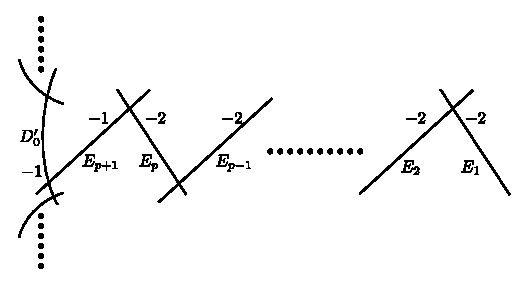
\includegraphics[scale=1.1]{figures/chap2-fig15.eps}
\end{figure}


\item Note that $P$ is a one-place point of $C$. We shall show that
  $C'$ meets $E_{p+1}$. Assume the contrary, \iec $E_{p+1}\cap
  C'=\phi$. Let $\Lambda'$ be the proper transform of $\Lambda$ by
  $\sigma$ and let $\Delta'$ be the member of $\Lambda'$ corresponding
  to $\Delta$. Then it is easily ascertained that:
\begin{itemize}
\item[$1^{\circ}$] $\Lambda'$ is spanned by $\Delta'$ and $C'$;

\item[$2^{\circ}$] $D'_{0}$ and $E_{p+1}$ are irreducible components
  of $\Delta'$;

\item[$3^{\circ}$] there exist no base points of $\Lambda'$ on $D'_{0}$ and $E_{p+1}$.
\end{itemize}
Let $\tau:V'\to \overline{V}$ be the contraction of $D'$, let
$\overline{\Lambda}$ be the proper transform of $\Lambda'$ and
$\overline{\Delta}:=\tau_{\ast}(\Delta')$ be the member of
$\overline{\Lambda}$ corresponding to $\Delta'$. Then
$\overline{\Delta}$ has three irreducible components meeting each
other in\pageoriginale\ one point, which is not a base point of
$\overline{\Lambda}$. This is a contradiction (\cf \ref{chap2:2.3},
(3)). Thus we know that $C'\cap E_{p+1}\neq \phi$.

\item With the notations of the step (II), we shall show that
  $E_{p+1}$ is not a component of $\Delta'$. Assume the contrary, and
  let $Q:=C'\cap E_{p+1}$. If $Q\neq D'_{0}\cap E_{p+1}$ we would have
  a contradiction by contracting $D'_{0}$ (\cf \ref{chap2:2.3}, (3)). Hence
  $Q=D'_{0}\cap E_{p+1}$. However this is again a contradiction
  because of the condition (3) above (\cf \ref{chap2:2.3}, (4)).

\item We shall show that $Q:=C'\cap E_{p+1}$ is distinct from
  $D'_{0}\cap E_{p+1}$ and $E_{P}\cap E_{p+1}$. Indeed, if
  $Q=D'_{0}\cap E_{p+1}$ we have a contradiction because of the
  condition (3) above (\cf \ref{chap2:2.3}, (4)). Assume that $Q=E_{P}\cap
  E_{p+1}$. Note that $E_{1},\ldots,E_{P}$ are contained in one and
  only one member of $\Lambda'$ other than $\Delta'$ because
  $E_{i}\cap \Supp(\Delta')=\phi$ for $1\leqq i\leqq p$. Then $Q$ is a
  base point of $\Lambda'$. This is a contradiction because $Q\not\in
  \Supp (\Delta')$.

\item From the above arguments we know that $E_{p+1}$ is a
  quasi-section of $\Lambda'$ such that
  $(\Delta'\cdot E_{p+1})=n_{0}$. Assume that $n_{0}>1$. Then we have a
  ramified covering $E_{p+1}\to \mathbb{P}^{1}_{k}$ of degree $n_{0}$,
  which ramifies totally over at least three points of
  $\mathbb{P}^{1}_{k}$. By Hurwitz's formula, we have:
$$
-2\geqq -2n_{0}+3(n_{0}-1)=n_{0}-3.
$$
This is a contradiction. Hence we obtain $n_{0}=1$.

\item Since $P$ is a one-place point of $C$, the fact that $E_{p+1}$
  is a quasi-section of $\Lambda'$ implies that $e=(p+1)\nu$ and
  $\nu=(C'\cdot E_{p+1})$. Since\pageoriginale\ $\nu=n_{0}=1$ we know
  that $e=p+1$.
\end{enumerate}
\end{proof}

\subsection{}\label{chap2:6.4}
In the paragraphs \ref{chap2:6.4} $\sim$ \ref{chap2:6.6}, let the notations and
assumptions be as in \ref{chap2:6.2}. Assume furthermore that $\Lambda$ has
a linear reducible member $\Delta$ whose weighted graph is the
following linear chain:
\begin{figure}[H]
\centering
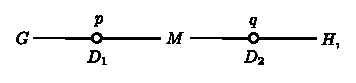
\includegraphics{figures/chap2-fig16.eps}
\end{figure}
\noindent
where $G$, $M$ and $H$ are given respectively by
\begin{figure}[H]
\centering
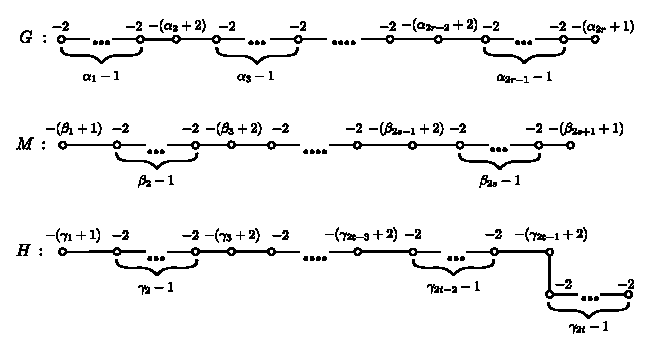
\includegraphics{figures/chap2-fig17.eps}
\end{figure}
\noindent
$\alpha_{i}$, $\beta_{j}$ and $\gamma_{\ell}$ being positive integers
for $1\leqq i\leqq 2r$, $1\leqq j\leqq 2s+1$ and $1\leqq \ell\leqq
2t$. $G$, $M$ and $H$ are called respectively {\em the left, the
  middle and the right branches} of the weighted graph of
$\Delta$. The absence of the left branch $G$ (or the middle branch
$M$, or the right branch $H$, \resp) is denoted by $G=\phi$ (or
$M=\phi$, or $H=\phi$, \resp). In the above graph the components of
$\Delta$ with self-intersection multiplicities $p$ and $q$ are denoted
respectively by $D_{1}$ and $D_{2}$. 

\subsection{}\label{chap2:6.5}
\begin{lemma*}
  Let\pageoriginale\ the notations and assumptions be as in \ref{chap2:6.2} and
  \ref{chap2:6.4}. Let $n_{i}(i=1,2)$ be the multiplicity of $D_{i}$ in
  $\Delta$. Assume that $B=\{P_{1},P_{2}\}$ with $P_{i}\in D_{i}$ and
  $P_{i}\not\in$ the components of $\Delta$ other than $D_{i}$ for
  $i=1,2$, that $n_{1}\neq 1$ and $n_{2}\neq 1$, and that either $p\leqq
  0$ or $q\leqq 0$. Then the following assertions hold true:
  \begin{enumerate}
    \renewcommand{\labelenumi}{\rm(\theenumi)}
  \item Either $p\geqq 0$ or $q\geqq 0$. Thus, in the assertions below
    we assume that $q\geqq 0$ and $p\leqq 0$.
    
  \item If $p<0$ and $q\geqq 0$ then $H=\phi$.
    
  \item If $p=0$ and $q\geqq 0$ then either $G=\phi$ or $H=\phi$.
  \end{enumerate}
\end{lemma*}

\begin{proof}
Let $C$ be a general member of $\Lambda$ and let $e_{i}:=(C\cdot
D_{i})=i(C,D_{i}$; $P_{i})$ and $\nu_{i}:=\mult_{P_{i}}C$ for $i=1,2$.
\begin{enumerate}
\renewcommand{\labelenumi}{\rm(\theenumi)}
\item The assertion (1) follows from Lemma \ref{chap2:2.3}, (4).

\item Consider first the case where $p<0$ and $q>0$. Assume that
  $H\neq \phi$. Then $D_{2}$ is not a terminal component of
  $\Delta$. Lemma \ref{chap2:6.3} then tells us that $n_{2}=1$, which
  contradicts the assumption. Hence $H=\phi$. Consider next the case
  where $p<0$ and $q=0$. Assume that $H\neq \phi$. Let $\sigma:V'\to
  V$ be the quadratic transformation of $V$ with center at
  $P_{2}$. Let $\Lambda':=\sigma'(\Lambda)$, $C':=\sigma'(C)$,
  $D'_{2}:=\sigma'(D_{2})$, $E:=\sigma^{-1}(P_{2})$, $Q:=E\cap C'$ and
  $\Delta':=$ the member of $\Lambda'$ corresponding to $\Delta$. Then
  $\Lambda'$ is spanned by $C'$ and $\Delta'$. We shall show that
  $Q\not\in D'_{2}$ and $E\not\subset \Supp(\Delta')$, which imply
  that $e_{2}=\nu_{2}=n_{2}$ and that $E$ is a quasi-section of
  $\Lambda'$ with $(C'\cdot E)=\nu_{2}$. If $Q\in D'_{2}$ then we
  would have a contradiction by Lemma \ref{chap2:2.3}, (4), regardless of
  whether or not $E\subset \Supp(\Delta')$. Thus $Q\not\in D'_{2}$. If
  $E\subset \Supp(\Delta')$ then we would have a contradiction by
  contracting $D'_{2}$ as in the proof of Lemma \ref{chap2:6.3},
  because\pageoriginale\ $D_{2}$ is not a terminal component of
  $\Delta$. Thus $E\not\subset \Supp(\Delta')$. Since every member of
  $\Lambda'$ has a one-place point on $E$ and the characteristic of
  $k$ is zero, $E$ must be a cross-section of $\Lambda'$, \iec
  $\nu_{2}=n_{2}=1$. This is a contradiction. Hence we have $H=\phi$. 

\item Assume that $G\neq \phi$ and $H\neq \phi$. We shall first
  consider the case where $p=0$ and $q>0$. Let $\sigma:V'\to V$ be the
  quadratic transformation of $V$ with center at $P_{1}$. Let
  $\Lambda':=\sigma'(\Lambda)$, $C':=\sigma'(C)$,
  $D'_{1}:=\sigma'(D_{1})$, $E:=\sigma^{-1}(P_{1})$, $Q:=E\cap C'$ and
  $\Delta':=$ the member of $\Lambda'$ corresponding to $\Delta$. Then
  $\Lambda'$ is spanned by $C'$ and $\Delta'$. We shall show that
  $Q\not\in D'_{1}$ and $E\nsubset \Supp(\Delta')$, which imply that
  $e_{1}=\nu_{1}=n_{1}$ and that $E$ is a quasi-section of $\Lambda'$
  with $(C'\cdot E)=\nu_{1}$. If $Q\in D'_{1}$, Lemma
  \ref{chap2:6.3}\footnote{If $E\nsubset \Supp(\Delta')$ we can apply
    Lemma \ref{chap2:6.3} in the stated form because $\Delta'$ is
    linear. However, if $E\subset \Supp(\Delta')$, we have to
    strengthen Lemma \ref{chap2:6.3} so as to apply it to the present
    situation. However, this is a very easy task; the given proof
    works without any modification.} applied to
  $(V',\Lambda',\Delta',D'_{2}:=\sigma'(D_{2}),P_{2})$ instead of
  $(V,\Delta,\Delta,D_{0},P)$ implies that $n_{2}=1$, which
  contradicts the assumption. Thus $Q\not\in D'_{1}$. If $E\subset
  \Supp(\Delta')$ we would have a contradiction by contracting
  $D'_{1}$ as in the proof of Lemma \ref{chap2:6.3}, because $D_{1}$ is
  not a terminal component of $\Delta$. Since every member of
  $\Lambda'$ has a one-place point on $E$ and the characteristic of
  $k$ is zero, $E$ must be a cross-section of $\Lambda'$, \iec
  $\nu_{1}=n_{1}=1$. This is a contradiction. Therefore, we know that
  either $G=\phi$ or $H=\phi$. consider next the case where
  $p=q=0$. Let $\sigma:V'\to V$ be the composition of quadratic
  transformations of $V$ with centers at $P_{1}$ and $P_{2}$. Let
  $\Lambda':=\sigma'(\Lambda)$, $C':=\sigma'(C)$,
  $D'_{i}:=\sigma'(D_{i})$, $E_{i}:=\sigma^{-1}(P_{i})$,
  $Q_{i}:=E_{i}\cap C'$ and $\Delta':=$ the member of $\Lambda'$
  corresponding to $\Delta$,\pageoriginale\ where $i=1,2$. We have only
  to show that either $Q_{1}\not\in D'_{1}$ and $E_{1}\not\subset
  \Supp(\Delta')$ or $Q_{2}\not\in D'_{2}$ and $E_{2}\not\in
  \Supp(\Delta')$; in either case we get a contradiction. If $Q_{i}\in
  D'_{i}(i=1,2)$ we have a contradiction by Lemma \ref{chap2:2.3} (4),
  regardless of whether or not $E_{i}\subset
  \Supp(\Delta')(i=1,2)$. Thus, either $Q_{1}\not\in D'_{1}$ or
  $Q_{2}\not\subset D'_{2}$. Assume that $Q_{1}\not\in D'_{1}$. Then
  $E_{1}\not\subset \Supp(\Delta')$, for, if otherwise, we would have
  a contradiction by contracting $D'_{1}$ because $D_{1}$ is not a
  terminal component of $\Delta$. Similarly, we have $E_{2}\not\subset
  \Supp(\Delta')$ if $Q_{2}\not\in D'_{2}$.
\end{enumerate}
\end{proof}

\subsection{}\label{chap2:6.6}
\begin{lemma*}
  Let the notations and assumptions be as in \ref{chap2:6.2} and
  \ref{chap2:6.4}. Assume that $B=\{P_{2}\}$ with $P_{2}\in D_{2}$ and
  $P_{2}\not\in$ the components of $\Delta$ other than $D_{2}$. Assume
  that the multiplicity $n_{2}$ of $D_{2}$ in $\Delta$ is not equal to
  $1$. Then the following assertions hold true:
  \begin{enumerate}
    \renewcommand{\labelenumi}{\rm(\theenumi)}
  \item $p<0$, and if $p\neq -1$ then $q\geqq 0$.
    
  \item If $p\leqq -2$ then $H=\phi$.
    
  \item If $p=-1$ then either $H=\phi$ or there exists a contraction
    $\rho$ of $V$ onto a nonsingular projective surface $W$ such that
    $\rho_{\ast}\Lambda$ is spanned by $\rho_{\ast}(C)$ and
    $\rho_{\ast}(\Delta)$ and that $\rho_{\ast}(\Delta)$ has the
    following weighted graph:
    \begin{figure}[H]
      \centering
      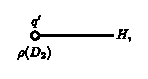
\includegraphics[scale=1.5]{figures/chap2-fig18.eps}
    \end{figure}
    \noindent
    where $H$ is the same graph as in \ref{chap2:6.4} and $q'=q+1$ or
    $q+\alpha_{1}+1$; in the second case, any component in the graphs $G$
    and $M$ as well as $D_{1}$ has multiplicity $>1$ in $\Delta$.
  \end{enumerate}
\end{lemma*}

\begin{proof}
Let $e_{2}:=(C\cdot D_{2})=i(C,D_{2};P_{2})$ and
$\nu_{2}:=\mult_{P_{2}}C$. 
\begin{enumerate}
\renewcommand{\labelenumi}{\rm(\theenumi)}
\item Since\pageoriginale\ $D_{1}\cap B=\phi$ we have $p=(D^{2}_{2})<0$
  (\cf \ref{chap2:2.3}, (1)). If $p\neq -1$ we must have $q\geqq 0$ by
  virtue of Lemma \ref{chap2:2.3}, (4).

\item Assume that $H\neq \phi$. Then $D_{2}$ is not a terminal
  component of $\Delta$. Since $n_{2}\neq 1$ we must have $q\leqq 0$
  (\cf Lemma \ref{chap2:6.3}). Since $q\geqq 0$ as shown above, we know
  that $q=0$. The same argument as used to prove the assertion (2) of
  Lemma \ref{chap2:6.5} leads us to a contradiction. Hence $H=\phi$.

\item Assume that $H\neq \phi$. Since $D_{1}$ is an exceptional
  component of $\Delta$, $D_{1}$ is contractible. After the
  contraction of $D_{1}$, if there exists a contractible component in
  the graphs $G$ and $M$, it must be either one of the components with
  weights $-(\alpha_{2r}+1)$ and $(-(\beta_{1}+1)$; the weights
  becoming $-\alpha_{2r}$ and $-\beta_{1}$ respectively after the
  contraction of $D_{1}$, we must have $\alpha_{2r}=1$ or
  $\beta_{1}=1$. If $\beta_{1}=1$ for instance, the $\beta_{2}$
  components in the graph $M$ with weights $-(\beta_{1}+1),
  -2,\ldots,-2$ respectively are contractible. After the contraction
  of these $\beta_{2}$ components, the component with weight
  $-(\alpha_{2r}+1)$ in the graph $G$ has a (new) weight
  $-(\alpha_{2r}-\beta_{2})$, and the component with weight
  $-(\beta_{3}+2)$ in the graph $M$ has a weight $-(\beta_{3}+1)$. If
  there exists still a contractible component in the graphs $G$ and
  $M$ after the contraction of $D_{1}$ and $\beta_{2}$ components in
  $M$, it must be the component with weight $-(\alpha_{2r}+1)$ in the
  graph $G$, \iec we must have $\alpha_{2r}=\beta_{2}+1$. Repeat the
  above argument, and let $\rho:V\to W$ be the contraction of all
  possible components in the graphs $G$ and $M$. The contraction
  $\rho$ is uniquely determined. It is clear that the proper transform
  $\rho_{\ast}(\Lambda)$ of $\Lambda$ by $\rho$ is spanned by
  $\rho(C)$ and $\rho_{\ast}(\Delta)$, and that $\rho_{\ast}(\Delta)$
  has the following weighted graph:
\begin{figure}[H]
\centering
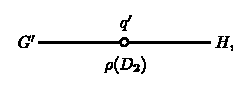
\includegraphics[scale=1.1]{figures/chap2-fig19.eps}
\end{figure}\pageoriginale\
\noindent
where $G'$ is the graph similar to $G$ and obtained in the
above-explained way by the contraction $\rho$ from the graph:
\begin{figure}[H]
\centering
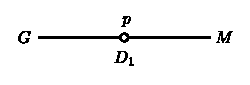
\includegraphics[scale=1.1]{figures/chap2-fig20.eps}
\end{figure}
\noindent
and where $q'\geqq q$, the inequality $q'>q$ taking place only if all
components of the graph $M$ are contracted by $\rho$. Note that
$\rho_{\ast}(\Lambda)$ has only one base point $\rho(P_{2})$, that
$e_{2}=(\rho(C)\cdot\rho(D_{2}))$ and
$\nu_{2}=\mult_{\rho(P_{2})}\rho(C)$ and that $n_{2}$ is the
multiplicity of $\rho(D_{2})$ in $\rho_{\ast}(\Delta)$. If $G'\neq
\phi$ then $H=\phi$ by virtue of the assertion (2) above. It is easily
verified that the case $G'=\phi$ occurs only in one of the following
four cases:
\begin{itemize}
\item[$1^{\circ}$] $s=r$; $\beta_{1}=1$, $\beta_{2}=\alpha_{2r-1}$,
  $\beta_{3}=\alpha_{2r-1},\ldots,\beta_{2r-1}=\alpha_{3}$,
  $\beta_{2r}=\alpha_{2}$, $\beta_{2r+1}=\alpha_{1}+1$; $q'=q+1$,

\item[$2^{\circ}$] $s=r$; $\beta_{1}=1$, $\beta_2= \alpha_{2r-1}$,
  $\beta_{3}=\alpha_{2r-1},\ldots,\beta_{2r-1}=\alpha_{3}$,
  $\beta_{2r}=\alpha_{2}-1$, $\beta_{2r+1}=1$; $q'=q+\alpha_{1}+1$,

\item[$3^{\circ}$] $s=r-1$; $\alpha_{2r}=1$, $\alpha_{2r-1}=\beta_{1}-1$,
  $\alpha_{2r-2}=\beta_{2},\ldots,\alpha_{3}=\beta_{2r-3}$,
  $\alpha_{2}=\beta_{2r-2}$, $\alpha_{1}=\beta_{2r-1}-1$; $q'=q+1$,

\item[$4^{\circ}$] $s=r-1$; $\alpha_{2r}=1$,
  $\alpha_{2r-1}=\beta_{1}-1$,
  $\alpha_{2r-2}=\beta_{2},\ldots,\alpha_{3}=\beta_{2r-3}$,
  $\alpha_{2}=\beta_{2r-2}+1$, $\beta_{2r-1}=1$; $q'=q+\alpha_{1}+1$.
\end{itemize}
The last assertion is clear because $n_{2}>1$ and the base point
$P_{2}$ lies on $D_{2}$ but not on the other components of
$\Delta$.
\end{enumerate}
\end{proof}

\subsection{}\label{chap2:6.7}
In\pageoriginale\ the paragraphs \ref{chap2:6.7} $\sim$ \ref{chap2:6.17} we shall
prove the ``if'' part of Theorem \ref{chap2:6.1}. Thus the conditions (1)
$\sim$ (3) of the theorem are always assumed to be satisfied. A useful
remark is that we may replace $f$ by $f-\alpha$ for a general element
$\alpha\in k$ if necessary, because if $f-\alpha=c(x^{d}y^{e}-1)$ for
$c\in k^{\ast}$ and coordinates $x$, $y$ of $\mathbb{A}^{2}_{k}$ then
$f=c'({x'}^{d}{y'}^{e}-1)$ for $c'\in k^{\ast}$ and coordinates $x'$,
$y'$ of $\mathbb{A}^{2}_{k}$. Thus we assume once for all that the
curve $C_{0}$ on $\mathbb{A}^{2}_{k}$ defined by $f=0$ has exactly two
places at infinity. Embed $\mathbb{A}^{2}_{k}:=\Spec(k[x,y])$ into
$\mathbb{P}^{2}_{k}$ as the complement of a line $\ell_{0}$, and let
$C$ be the closure of $C_{0}$ on $\mathbb{P}^{2}_{k}$. We shall first
prove the following:

\begin{lemma*}
Assume that $C$ intersects $\ell_{0}$ in only one point $P_{0}$. Let
$d_{1}:=\mult_{P_{0}}C$. Then there exists a birational automorphism
$\rho$ of $\mathbb{P}^{2}_{k}$ such that $\rho$ induces a biregular
automorphism on $\mathbb{A}^{2}_{k}:=\mathbb{P}^{2}_{k}-\ell_{0}$ and
that the proper transform $C'$ of $C$ by $\rho$ intersects $\ell_{0}$
in two distinct points with $(C'\cdot\ell_{0})\leqq d_{1}$.
\end{lemma*}

\begin{proof}
Our proof consists of four subparagraphs \ref{chap2:6.7.1} $\sim$ \ref{chap2:6.7.4}.
\end{proof}

\subsubsection{}\label{chap2:6.7.1}
Set $d_{0}:=(C\cdot\ell_{0})$. Let $\Lambda$ be a linear pencil on
$\mathbb{P}^{2}_{k}$ spanned by $C$ and $d_{0}\ell_{0}$. Let
$V_{0}:=\mathbb{P}^{2}_{k}$ and let $\sigma_{1}:V_{1}\to V_{0}$ be the
quadratic transformation of $V_{0}$ with center at $P_{0}$. Let
$\ell^{(1)}_{0}:=\sigma'_{1}(\ell_{0})$,
$\ell_{1}:=\sigma^{-1}_{1}(P_{0})$, $C^{(1)}:=\sigma'_{1}(C)$ and
$\Lambda^{(1)}:=\sigma'_{1}(\Lambda)$. {\em We shall show that}
$d_{0}>d_{1}$. Assume the contrary: $d_{0}=d_{1}$. Then the linear
pencil $\Lambda^{(1)}$ is spanned by $C^{(1)}$ and
$d_{0}\ell_{0}^{(1)}$, and since
$(C^{(1)}\cdot\ell_{0}^{(1)})=d_{0}-d_{1}=0$ the pencil has no base
points. Hence $\Lambda^{(1)}$ defines a fibration
$\varphi_{1}:V_{1}\to \mathbb{P}^{1}_{k}$ whose general fibers are
isomorphic to $\mathbb{P}^{1}_{k}$. Then $d_{0}=1$ by virtue of Lemma
\ref{chap2:2.2}, (1). However this is impossible\pageoriginale\ because
$C$ has two distinct places on $\ell_{0}$. Therefore we know that
$d_{0}>d_{1}$. 

\subsubsection{}\label{chap2:6.7.2}
We shall prove the following assertion:

{\em Either $C^{(1)}$ intersects $\ell_{1}$ in two distinct points, or
  there exists a birational automorphism $\rho$ of
  $\mathbb{P}^{2}_{k}$ such that $\rho$ induces a biregular
  automorphism on $\mathbb{A}^{2}_{k}:=\mathbb{P}^{2}_{k}-\ell_{0}$
  and that $(C'\cdot\ell_{0})\leqq d_{1}<d_{0}$ where $C'$ is the
  proper transform of $C$ by $\rho$.}

\begin{proof}
Our proof consists of four steps.
\begin{enumerate}
\renewcommand{\theenumi}{\Roman{enumi}}
\renewcommand{\labelenumi}{\rm(\theenumi)}
\item Assume that $C^{(1)}$ intersects $\ell_{1}$ in a single point
  $P_{1}$. Then $P_{1}=\ell^{(1)}_{0}\cap \ell_{1}$ because
  $d_{0}>d_{1}$. Let $\sigma_{2}:V_{2}\to V_{1}$ be the quadratic
  transformation of $V_{1}$ with center at $P_{1}$. Let
  $\ell^{(2)}_{0}:=\sigma'_{2}(\ell^{(1)}_{0})\ell^{(2)}_{1}:=\sigma'_{2}(\ell_{1})$,
  $\ell_{2}=\ell^{(2)}_{2}:=\sigma^{-1}_{2}(P_{1})$,
  $C^{(2)}:=\sigma'_{2}(C^{(1)})$ and
  $\Lambda^{(2)}:=\sigma'_{2}(\Lambda^{(1)})$. Let
  $d_{2}:=\mult_{P_{1}}C^{(1)}$. Then it is easy to see that
  $\Lambda^{(2)}$ is spanned by $C^{(2)}$ and
  $d_{0}\ell_{0}^{(2)}+(d_{0}-d_{1})\ell^{(2)}_{1}+(2d_{0}-d_{1}-d_{2})\ell^{(2)}_{2}$,
  where $2d_{0}-d_{1}-d_{2}>0$ because
  $\ell^{(2)}_{0}\cap\ell^{(2)}_{1}=\phi$. Note that $d_{2}\leqq
  d_{1}$ and $d_{2}\leqq d_{0}-d_{1}$ because $(C^{(1)}\cdot
  \ell_{0}^{(1)})=d_{0}-d_{1}$ and $(C^{(1)}\cdot\ell_{1})=d_{1}$. If
  $d_{0}-d_{1}>d_{2}$ then
  $(C^{(2)}\cdot\ell^{(2)}_{0})=d_{0}-d_{1}-d_{2}>0$,
  $(C^{(2)}\cdot\ell^{(2)}_{2})=d_{2}>0$ and
  $((\ell^{(2)}_{0})^{2})=-1$. However this is impossible by virtue of
  Lemma \ref{chap2:2.3}, (4). Hence we have $d_{2}=d_{0}-d_{1}\leqq
  d_{1}$. By virtue of Lemma \ref{chap2:2.3}, (4) we know that $C^{(2)}$
  intersects $\ell_{2}$ in a single point $Q$. Indeed, if otherwise
  $C^{(2)}$ intersects $\ell_{2}$ in two distinct points $Q$ and $Q'$,
  where neither $Q$ nor $Q'$ lie on $\ell^{(2)}_{0}$; then contract
  $\ell^{(2)}_{0}$ and blow up the points $Q$ and $Q'$; this operation
  leads us to a contradiction. If $Q\neq \ell^{(2)}_{1}\cap \ell_{2}$
  then $d_{1}=d_{2}$, whence $d_{0}=2d_{1}$. If\pageoriginale\
  $d_{1}>d_{2}$ then $Q=P_{2}:=\ell^{(2)}_{1}\cap \ell_{2}$.

\item Write $d_{1}=q_{2}d_{2}+d_{3}$ with integers $q_{2}$, $d_{3}$
  such that $0\leqq d_{3}<d_{2}$ and $q_{2}\geqq 1$. For $2\leqq
  i\leqq q_{2}+1$ define $V^{(i)}$, $\sigma_{i}$,
  $\ell^{(i)}_{j}(0\leqq j\leqq i)$, $C^{(i)}$, $\Lambda^{(i)}$ and
  $P_{i}$ inductively as follows: Let $\sigma_{i}:V^{(i)}\to
  V^{(i-1)}$ be the quadratic transformation of $V^{(i-1)}$ with
  center at $P_{i-1}$ and let
  $\ell^{(i)}_{j}:=\sigma'_{i}(\ell^{(i-1)}_{j})$ for $0\leqq j\leqq
  i-1$, $\ell^{(i)}_{i}=\ell_{i}:=\sigma^{-1}_{i}(P_{i-1})$,
  $C^{(i)}:=\sigma'_{i}(C^{(i-1)})$,
  $\Lambda^{(i)}:=\sigma'_{i}(\Lambda^{(i-1)})$ and
  $P_{i}:=\ell^{(i)}_{1}\cap \ell_{i}$. By induction on $i(2\leqq
  i\leqq q_{2}+1)$ we shall show the following assertions:  

  $A_{1}(i):\Lambda^{(i)}$ is spanned by $C^{(i)}$ and 
  $d_{0}\ell_{0}^{(i)}+(d_{0}- d_{1})\ell_{1}^{(i)}+
  d_{0}(\ell^{(i)}_{2} +\cdots+\ell_{i}^{(i)})$,  

$A_{2}(i):(C^{(i)}\cdot \ell^{(i)}_{j})=0$ if $0\leqq j\leqq i-1$ and
  $j\neq 1$; $(C^{(i)}\cdot \ell^{(i)}_{1})=d_{1}-(i-1)d_{2}$;
  $(C^{(i)}\cdot \ell^{(i)}_{i})=d_{2}$;
  $\cup^{i}_{j=0}\ell^{(i)}_{j}$ has the following weighted graph:
\begin{figure}[H]
\centering
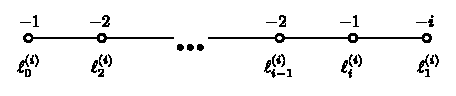
\includegraphics[scale=1.1]{figures/chap2-fig21.eps}
\end{figure}
\noindent
$A_{3}(i):C^{(i)}$ intersects $\ell_{i}$ in a single point $Q$, where
$Q=P_{i}$ if either $2\leqq i\leqq q_{2}$ or $i=q_{2}+1$ and $d_{3}>0$.

Indeed, the assertions $A_{1}(2)\sim A_{3}(2)$ are verified in the
step (I) above. Assuming that $A_{1}(j)\sim A_{3}(j)$ are verified for
$2\leqq j<i$ we shall prove $A_{1}(i)\sim A_{3}(i)$. Let
$\mu:=\mult_{P_{i-1}}C^{(i-1)}$. Then $\mu\leqq d_{2}$ and $\mu\leqq
d_{1}-(i-2)d_{2}$, and $\Lambda^{(i)}$ is spanned by $C^{(i)}$ and
$d_{0}\ell_{0}^{(i)}+(d_{0}-d_{1})\ell^{(i)}_{1}+d_{0}(\ell^{(i)}_{2}+
\cdots+\ell^{(i)}_{i-1})+(2d_{0}-d_{1}-\mu)\ell^{(i)}_{i}$,
where $2d_{0}-d_{1}-\mu>0$ because\pageoriginale\ $\ell^{(i)}_{1}\cap
\ell^{(i)}_{i-1}=\phi$. Suppose that $d_{2}>\mu$. Then the contraction
of $\ell^{(i)}_{0}$, $\ell^{(i)}_{2},\ldots,\ell^{(i)}_{i-2}$ leads us
to a contradiction by virtue of Lemma \ref{chap2:2.3}, (4). Hence
$d_{2}=\mu$ and $2d_{0}-d_{1}-\mu=d_{0}$. Thus $A_{1}(i)$ is
proved. By virtue of Lemma \ref{chap2:2.3}, (4) again, we know that
$C^{(i)}$ intersects $\ell_{i}$ in a single point $Q$. Indeed, if
otherwise $C^{(i)}$ intersects $\ell_{i}$ in two distinct points $Q$
and $Q'$, where neither $Q$ nor $Q'$ lie on $\ell^{(i)}_{i-1}$; then
contract $\ell^{(i)}_{0},\ldots,\ell^{(i)}_{i-1}$ and blow up the
points $Q$ and $Q'$; this operation leads us to a contradiction. If
$Q\neq P_{i}$ then
$(C^{(i)}\cdot\ell^{(i)}_{1})=d_{1}-(i-2)d_{2}-\mu=d_{1}-(i-1)d_{2}=0$,
\iec $i=q_{2}+1$ and $d_{3}=0$. Hence if either $2\leqq i\leqq q_{2}$
or $i=q_{2}+1$ and $d_{3}>0$ then $Q=P_{i}$ and $(C^{(i)}\cdot
\ell^{(i)}_{1})=d_{1}-(i-1)d_{2}$. Therefore, $A_{2}(i)$ and
$A_{3}(i)$ are proved.

\item We shall show that $d_{3}=0$. Assume the contrary:
  $d_{3}>0$. Set $r:=q_{2}+1$. Let $\sigma_{r+1}:V_{r+1}\to V_{r}$ be
  the quadratic transformation of $V_{r}$ with center at $P_{r}$, and
  let $\ell^{(r+1)}_{j}:=\sigma'_{r+1}(\ell^{(r)}_{j})$ for $0\leqq
  j\leqq r$, $\ell_{r+1}:=\sigma^{-1}_{r+1}(P_{r})$,
  $C^{(r+1)}:=\sigma'_{r+1}(C^{(r)})$ and
  $\Lambda^{(r+1)}:=\sigma'_{r+1}(\Lambda^{(r)})$. Let
  $\nu:=\mult_{P_{r}}C^{(r)}$. Then $\nu\leqq d_{3}<d_{2}$ because
  $(C^{(r)}\cdot \ell^{(r)}_{1})=d_{3}<d_{2}$, and $\Lambda^{(r+1)}$
  is spanned by $C^{(r+1)}$ and
  $d_{0}\ell_{0}^{(r+1)}+(d_{0}-d_{1})\ell^{(r+1)}_{1}+d_{0}(\ell_{2}^{(r+1)}+\cdots+\ell_{r}^{(r+1)})+(2d_{0}-d_{1}-\nu)\ell_{r+1}$
  with $2d_{0}-d_{1}-\nu>0$. Since $(C^{(r+1)}\cdot
  \ell^{(r+1)}_{r})=d_{2}-\nu>0$, $(C^{(r+1)}\cdot\ell_{r+1})=\nu>0$
  and $((\ell_{1}^{(r+1)})^{2})=-(r+1)<-2$ the contraction of
  $\ell_{0}^{(r+1)}$, $\ell^{(r+1)}_{2},\ldots,\ell^{(r+1)}_{r-1}$
  leads us to a contradiction by virtue of Lemma \ref{chap2:2.3},
  (4). Hence $d_{3}=0$. Thence $d_{0}=rd_{2}$ and
  $d_{1}=(r-1)d_{2}$. We reached to the following configuration:
\begin{figure}[H]
\centering
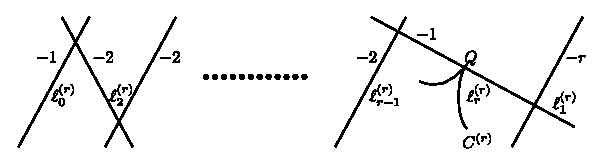
\includegraphics[scale=1.1]{figures/chap2-fig22.eps}
\end{figure}\pageoriginale\


\item We set $\overline{V}_{0}:=V_{r}$,
  $\overline{\ell}_{0}:=\ell_{r}$, $\overline{C}:=C^{(r)}$,
  $\overline{P}_{0}:=Q$ and
  $\overline{\Lambda}:=\overline{\Lambda}^{(0)}:=\Lambda^{(r)}$. Let
  $\overline{\sigma}_{1}:\overline{V}_{1}\to \overline{V}_{0}$ be the
  quadratic transformation of $\overline{V}_{0}$ with center at
  $\overline{P}_{0}$, and let
  $\overline{\ell}^{(1)}_{0}:=\overline{\sigma}'_{1}(\overline{\ell}_{0})$,
  $\overline{\ell}_{1}^{(1)}:=\overline{\sigma}^{-1}_{1}(\overline{P}_{0})$,
  $\overline{C}^{(1)}=\overline{\sigma}'(\overline{C})$ and
  $\overline{\Lambda}^{(1)}=\overline{\sigma}'_{1}(\overline{\Lambda})$. By
  abuse of notations, we denote
  $\overline{\sigma}'_{1}(\ell_{j}^{(r)})$ by $\ell^{(r)}_{j}$ again
  for $0\leqq j\leqq r$. Let
  $\mu_{0}:=\mult_{\overline{P}_{0}}\overline{C}$. Then $\mu_{0}\leqq
  d_{2}$, and $\overline{\Lambda}^{(1)}$ is spanned by
  $\overline{C}^{(1)}$ and
  $d_{0}\ell_{0}^{(r)}+(d_{0}-d_{1})\ell_{1}^{(r)}+d_{0}(\ell^{(r)}_{2}+\cdots+\ell^{(r)}_{r})+(d_{0}-\mu_{0})\overline{\ell}_{1}$. If
  $\mu_{0}<d_{2}$ the contraction of $\ell^{(r)}_{0}$,
  $\ell^{(r)}_{2},\ldots,\ell^{(r)}_{r-1}$ leads us to a contradiction
  by Lemma \ref{chap2:2.3}, (4). Thus $\mu_{0}=d_{2}$. If $r>2$,
  $\overline{C}^{(1)}$ intersects $\overline{\ell}_{1}$ in a single
  point $\overline{Q}_{1}$; indeed, if otherwise, the contraction of
  $\ell^{(r)}_{0}$, $\ell^{(r)}_{2},\ldots,\ell^{(r)}_{r}$ and
  blowings-up of two points in $\overline{C}^{(1)}\cap
  \overline{\ell}_{1}$ leads us to a contradiction by Lemma
  \ref{chap2:2.3}, (4). For $1\leqq i\leqq r-2$, assume that we obtained
  inductively $\overline{V}_{i}$, $\overline{\sigma}_{i}$,
  $\overline{\ell}^{(i)}_{j}(0\leqq j\leqq i)$, $\ell^{(r)}_{s}(0\leqq
  s\leqq r)$, $\overline{C}^{(i)}$ and $\overline{\Lambda}^{(i)}$,
  where;
\begin{enumerate}
\renewcommand{\theenumii}{\arabic{enumii}}
\renewcommand{\labelenumii}{(\theenumii)}
\item $\overline{\sigma}_{i}:\overline{V}_{i}\to \overline{V}_{i-1}$
  is the quadratic transformation of $\overline{V}_{i-1}$,

\item $\overline{\Lambda}^{(i)}$ is spanned by $\overline{C}^{(i)}$
  and
  $d_{0}\ell^{(r)}_{0}+(d_{0}-d_{1})\ell^{(r)}_{1}+d_{0}(\ell^{(r)}_{2}+\cdots+\ell^{(r)}_{r})+(d_{0}-d_{2})\overline{\ell}^{(i)}_{1}+(d_{0}-2d_{2})\overline{\ell}^{(i)}_{2}+\cdots+(d_{0}-id_{2})\overline{\ell}^{(i)}_{i}$,

\item $\overline{C}^{(i)}$ intersects
  $\overline{\ell}_{i}:=\overline{\ell}^{(i)}_{i}$ in a single point
  $\overline{P}_{i}$ with
  $(\overline{C}^{(i)}\cdot\overline{\ell}_{i})=d_{2}$ and
  $\mu_{i}=\mult_{\overline{P}_{i}}\overline{C}^{(i)}$, where
  $\overline{P}_{i}\not\in\overline{\ell}^{(i)}_{i-1}$. 
\end{enumerate}
Let $\overline{\sigma}_{i+1}:\overline{V}_{i+1}\to \overline{V}_{i}$
be the quadratic transformation of $\overline{V}_{i}$
with\pageoriginale\ center at $\overline{P}_{i}$, and let
$\overline{\ell}_{j}^{(i+1)}:=\overline{\sigma}'_{i+1}(\overline{\ell}^{(i)}_{j})$
for $0\leqq j\leqq i$,
$\overline{\ell}_{i+1}:=\overline{\ell}^{(i+1)}_{i+1}:=\overline{\sigma}^{-1}_{i+1}(\overline{P}_{i})
\overline{C}^{(i+1)}:=\overline{\sigma}'_{i+1}(\overline{C}^{(i)})$
and
$\overline{\Lambda}^{(i+1)}:=\overline{\sigma}'_{i+1}(\overline{\Lambda}^{(i)})$. By
abuse of notations we denote
$\overline{\sigma}'_{i+1}(\ell^{(r)}_{s})$ by $\ell^{(r)}_{s}$ again
for $0\leqq s\leqq r$. Then $\mu_{i}\leqq d_{2}$, and
$\overline{\Lambda}^{(i+1)}$ is spanned by $\overline{C}^{(i+1)}$ and
$d_{0}\ell_{0}^{(r)}+(d_{0}-d_{1})\ell^{(r)}_{1}+d_{0}(\ell^{(r)}_{2}+\cdots+\ell^{(r)}_{r})+(d_{0}-d_{2})\overline{\ell}_{1}^{(i+1)}+\cdots+(d_{0}-id_{2})\overline{\ell}_{i}^{(i+1)}+(d_{0}-id_{2}-\mu_{i})\overline{\ell}_{i+1}$. If
$\mu_{i}<d_{2}$ the contraction of $\ell^{(r)}_{0}$,
$\ell^{(r)}_{2},\ldots,\ell^{(r)}_{r},\overline{\ell}_{1}^{(i+1)},\ldots,\overline{\ell}^{(i+1)}_{i-1}$
leads us to a contradiction by virtue of Lemma \ref{chap2:2.3},
(4). Hence $\mu_{i}=d_{2}$. If $i\leqq r-3$, $\overline{C}^{(i+1)}$
intersects $\overline{\ell}_{i+1}$ in a single point
$\overline{P}_{i+1}(\not\in \overline{\ell}_{i}^{(i+1)})$; indeed, if
otherwise, the contraction of $\ell^{(r)}_{0}$,
$\ell^{(r)}_{2},\ldots,\ell^{(r)}_{r},\overline{\ell}_{1}^{(i+1)},\ldots,\overline{\ell}_{i}^{(i+1)}$
and blowings-up of two points in $\overline{C}^{(i+1)}\cap
\overline{\ell}_{i+1}$ lead us to a contradiction by Lemma
\ref{chap2:2.3}, (4). continuing the above argument we obtain the
following configuration on $\overline{V}^{(r-1)}$:
\begin{figure}[H]
\centering
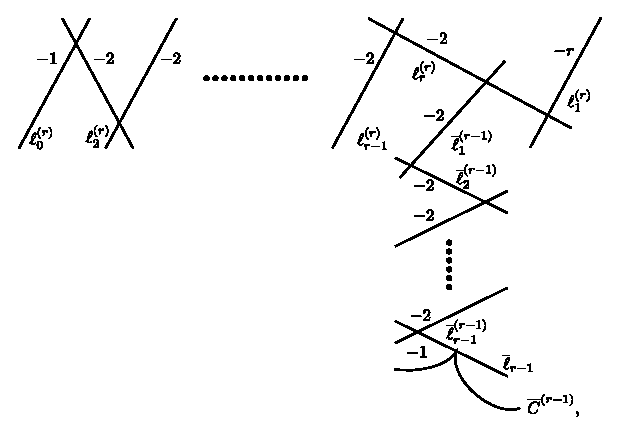
\includegraphics{figures/chap2-fig23.eps}
\end{figure}
where:\pageoriginale\
\begin{enumerate}
\renewcommand{\theenumii}{\roman{enumii}}
\renewcommand{\labelenumii}{\rm(\theenumii)}
\item $\overline{\Lambda}^{(r-1)}$ is spanned by
  $\overline{C}^{(r-1)}$ and
  $d_{0}\ell_{0}^{(r)}+(d_{0}-d_{1})\ell^{(r)}_{1}+d_{0}(\ell^{(r)}_{2}+\cdots+\ell^{(r)}_{r})+(d_{0}-d_{2})\overline{\ell}_{1}^{(r-1)}+\cdots+(d_{0}-(r-1)d_{2})\overline{\ell}^{(r-1)}_{r-1}$, 

\item $(\overline{C}^{(r-1)}\cdot \overline{\ell}_{r-1})=d_{2}$ and
  $(\overline{C}^{(r-1)}\cdot \overline{\ell}^{(r-1)}_{r-2})=0$. 
\end{enumerate}
\end{enumerate}

Let $\sigma:\overline{V}^{(r-1)}\to \mathbb{P}^{2}_{k}$ be the
composition $\sigma:=(\sigma_{1}\ldots\sigma_{r}\cdot
\overline{\sigma}_{1}\ldots\overline{\sigma}_{r-1})$ and let
$\tau:\overline{V}^{(r-1)}\to \mathbb{P}^{2}_{k}$ be the contraction
of
$\ell^{(r)}_{0},\ell^{(r)}_{2},\ldots,\ell^{(r)}_{r},\overline{\ell}^{(r-1)}_{1},\ldots$,
$\overline{\ell}^{(r-1)}_{r-2}$
and $\ell^{(r)}_{1}$ in this order. Then $\rho:=\tau\cdot\sigma^{-1}$
is a birational automorphism on $\mathbb{P}^{2}_{k}$ such that $\rho$
induces a biregular automorphism on
$\mathbb{A}^{2}_{k}:=\mathbb{P}^{2}_{k}-\ell_{0}$ and that
$(C'\cdot\ell_{0})=(\overline{C}^{(r-1)}\cdot\overline{\ell}_{r-1})=d_{2}\leqq
d_{1}$, where $C'$ is the proper transform of $C$ by $\rho$. This
completes a proof of \ref{chap2:6.7.2}.
\end{proof}

\subsubsection{}\label{chap2:6.7.3}
We shall prove the following assertion:

{\em Assume that $C^{(1)}$ intersects $\ell_{1}$ in two distinct
  points $P_{1}$ and $P'_{1}$. Then there exists a birational
  automorphism $\rho$ of $\mathbb{P}^{2}_{k}$ such that $\rho$ induces
  a biregular automorphism on
  $\mathbb{A}^{2}_{k}:=\mathbb{P}^{2}_{k}-\ell_{0}$ and that $C'$
  intersects $\ell_{0}$ in two distinct points, where $C'$ is the
  proper transform of $C$ by $\rho$. Moreover, $(C'\cdot\ell_{0})\leqq
  d_{1}$.}

\begin{proof}
Our proof consists of four steps.
\begin{enumerate}
\renewcommand{\theenumi}{\Roman{enumi}}
\renewcommand{\labelenumi}{\rm(\theenumi)}
\item One of $P_{1}$ and $P'_{1}$, say $P_{1}$, must be the point
  $\ell^{(1)}_{0}\cap \ell_{1}$; indeed, if otherwise, the pencil
  $\Lambda^{(1)}$ spanned by $C^{(1)}$ and
  $d_{0}\ell^{(1)}_{0}+(d_{0}-d_{1})\ell_{1}$ has no base points on
  $\ell^{(1)}_{0}$, which is a contradiction by virtue of Lemma
  \ref{chap2:2.3}, (1) because $((\ell^{(1)}_{0})^{2})=0$. Moreover, both
  $P_{1}$ and $P'_{1}$ are one-place points of $C^{(1)}$. Let
  $\mu_{1}:=i(C^{(1)},\ell_{1};p_{1})$ and
  $\mu'_{1}:=i(C^{(1)},\ell_{1};p'_{1})$. Then
  $d_{1}=\mu_{1}+\mu'_{1}$. {\em We shall show\pageoriginale\ that}
  $\mult_{P_{1}}C^{(1)}=(C^{(1)}\cdot\ell^{(1)}_{0})=d_{0}-d_{1}\leqq
  \mu_{1}$. Indeed, let $\sigma_{2}:V_{2}\to V_{1}$ be the quadratic
  transformation of $V_{1}$ with center at $P_{1}$, and let
  $\ell^{(2)}_{j}:=\sigma'_{2}(\ell^{(1)}_{j})(j=0,1)$,
  $\ell_{2}:=\ell^{(2)}_{2}:=\sigma^{-1}_{2}(P_{1})$,
  $C^{(2)}:=\sigma'_{2}(C^{(1)})$, and
  $\Lambda^{(2)}:=\sigma'_{2}(\Lambda^{(1)})$. Let
  $\nu_{1}:=\mult_{P_{1}}C^{(1)}$. Then $\nu_{1}\leqq
  (C^{(1)}\cdot\ell^{(1)}_{0})$, $\nu_{1}\leqq \mu_{1}$, and
  $\Lambda^{(2)}$ is spanned by $C^{(2)}$ and
  $d_{0}\ell_{0}^{(2)}+(d_{0}-d_{1})\ell^{(2)}_{1}+(2d_{0}-d_{1}-\nu_{1})\ell_{2}$. Since
  $(C^{(2)}\cdot \ell^{(2)}_{0})=(C^{(1)}\cdot
  \ell^{(1)}_{0})-\nu_{1}$, $(C^{(2)}\cdot\ell_{2})=\nu_{1}>0$ and
  $((\ell^{(2)}_{1})^{2})=-2$, the equality $\nu_{1}=(C^{(1)}\cdot
  \ell^{(1)}_{0})$ is implied by Lemma \ref{chap2:2.3}, (4).

\item Set $d_{2}:=\nu_{1}$\footnote{Note that $d_{0}=d_{1}+d_{2}$ and
  $d_{2}<d_{1}=\mu_{1}+\mu'_{1}$.} and write
  $d_{1}-\mu'_{1}=\mu_{1}=qd_{2}+d'_{3}$ with integers $q$, $d'_{3}$
  such that $0\leqq d'_{3}<d_{2}$ and $q\geqq 1$. For $2\leqq i\leqq
  q+1$ define $V^{(i)}$, $\sigma_{i}$, $\ell^{(i)}_{j}(0\leqq j\leqq
  i)$, $C^{(i)}$, $\Lambda^{(i)}$ and $P_{i}$ inductively as follows:
  Let $\sigma_{i}:V^{(i)}\to V^{(i-1)}$ be the quadratic
  transformation of $V^{(i-1)}$ with center at $P_{i-1}$, and let
  $\ell^{(i)}_{j}:=\sigma'_{i}(\ell^{(i-1)}_{j})$ for $0\leqq j\leqq
  i-1$, $\ell_{i}:=\ell^{(i)}_{i}:=\sigma^{-1}_{i}(P_{i-1})$,
  $C^{(i)}:=\sigma'_{i}(C^{(i-1)})$,
  $\Lambda^{(i)}:=\sigma'_{i}(\Lambda^{(i-1)})$ and
  $P_{i}:\ell^{(i)}_{1}\cap \ell_{i}$. By induction on $i(2\leqq
  i\leqq q+1)$ we can show the following assertions:

$A'_{1}(i):\Lambda^{(i)}$ is spanned by $C^{(i)}$ and
  $d_{0}\ell_{0}^{(i)}+(d_{0}-d_{1})\ell^{(i)}_{1}+d_{0}(\ell^{(i)}_{2}+\cdots+\ell^{(i)}_{i})$,

$A'_{2}(i):(C^{(i)}\cdot\ell^{(i)}_{j})=0$ if $0\leqq j\leqq i-1$ and
  $j\neq 1$; $i(C^{(i)},\ell^{(i)}_{1};P_{i})=\mu_{1}-(i-1)d_{2}$;
  $(C^{(i)}\cdot\ell_{i})=d_{2}$;
  ${\displaystyle{\mathop{\bigcup}^{i}_{j=0}}}\ell^{(i)}_{j}$ has the
  following weighted graph:
\begin{figure}[H]
\centering
\includegraphics{figures/chap2-fig24.eps}
\end{figure}
$A'_{3}(i):C^{(i)}$ intersects $\ell_{i}$ in a single point $Q$, where
$Q=P_{i}$\pageoriginale\ if either $2\leqq i\leqq q$ or $i=q+1$ and
$d'_{3}>0$.

The proof is the same as that of the step (II) of \ref{chap2:6.7.2} up to a
slight modification caused by difference of the situations. Hence we
leave the readers a task to reproduce it.

\item By the same argument as in the proof of the step (III) of
  \ref{chap2:6.7.2}, we can show that $d'_{3}=0$. Then, setting $r=q+1$, we
  have $\mu_{1}=(r-1)d_{2}$, $d_{1}=(r-1)d_{2}+\mu'_{1}$ and
  $d_{0}=rd_{2}+\mu'_{1}$, where $\mu'_{1}>0$. We have the following
  configuration on $V^{(r)}$:
\begin{figure}[H]
\centering
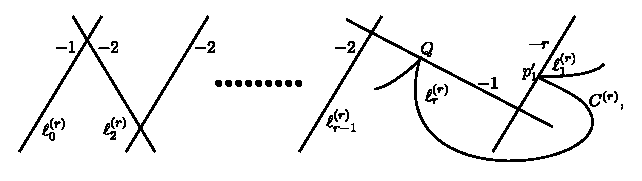
\includegraphics{figures/chap2-fig25.eps}
\end{figure}
where $(C^{(r)}\cdot\ell^{(r)}_{r})=d_{2}$ and
$(C^{(r)}\cdot\ell^{(r)}_{1})=\mu'_{1}$. 

\item Starting with the quadratic transformation of $V^{(r)}$ with
  center at $Q$ and following the argument in the step (IV) of the
  proof of \ref{chap2:6.7.2} we obtain the surface $\overline{V}^{(r-1)}$
  and the configuration on it: See the next page, where
  $(\overline{C}^{(r-1)}\cdot \overline{\ell}_{r-1})=d_{2}$ and
  $(\overline{C}^{(r-1)}\cdot\ell^{(r)}_{1})=\mu'_{1}$. Let $\sigma$,
  $\tau:\overline{V}^{(r-1)}\to \mathbb{P}^{2}_{k}$ be as defined as
  in the step (IV) of \ref{chap2:6.7.2} and let
  $\rho=\tau\cdot\sigma^{-1}$. Then $\rho$ is a birational
  automorphism of $\mathbb{P}^{2}_{k}$ such that $\rho$ induces a
  biregular automorphism on
  $\mathbb{A}^{2}_{k}:=\mathbb{P}^{2}_{k}-\ell_{0}$ and that
  $(C'\cdot\ell_{0})=d_{2}+\mu'_{1}\leqq d_{1}$, where $C'$ is the
  proper transform of $C$ by $\rho$. Apparently, $C'$ intersects
  $\ell_{0}$ in two distinct points. This completes a proof of
  \ref{chap2:6.7.3}.
\begin{figure}[H]
\centering
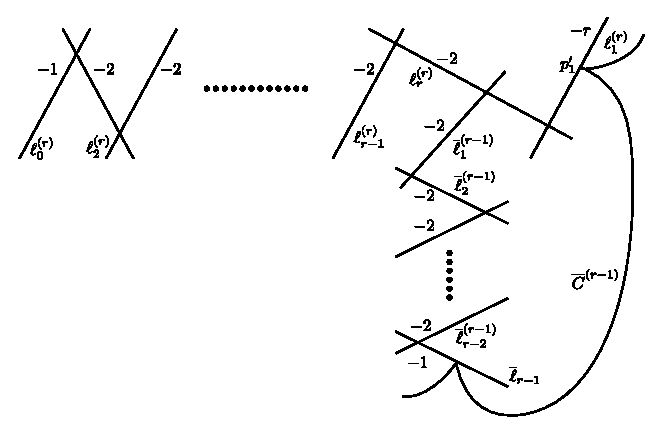
\includegraphics[scale=.95]{figures/chap2-fig26.eps}
\end{figure}\pageoriginale\

\centerline{ (The configuration in the step (IV) of \ref{chap2:6.7.3})}
\end{enumerate}
\end{proof}

\subsubsection{}\label{chap2:6.7.4}
It is now apparent that we can finish our proof of Lemma \ref{chap2:6.7}
by induction on $d_{0}:=(C\cdot\ell_{0})$ and by making use of
\ref{chap2:6.7.2} and \ref{chap2:6.7.3}. As the proofs of \ref{chap2:6.7.2} and
\ref{chap2:6.7.3} indicate, we have the following remark:

\begin{remark*}
Let $C$, $\ell_{0}$, $\rho$ and $C'$ be as in Lemma \ref{chap2:6.7}. Let
$d_{0}:=(C\cdot\ell_{0})$ and $d'_{0}:=(C'\cdot\ell_{0})$. Let
$\Lambda$ be the linear pencil on $\mathbb{P}^{2}_{k}$ spanned by $C$
and $d_{0}\ell_{0}$, and let $\Lambda'$ be the linear pencil on
$\mathbb{P}^{2}_{k}$ spanned by $C'$ and $d'_{0}\ell_{0}$. Then
$\Lambda'$ is the proper transform of $\Lambda$ by $\rho$. In
particular, if $f'$ is an irreducible element of $k[x,y]$ defining
$C'\cap \mathbb{A}^{2}_{k}$ and $C'_{\alpha}$ is the curve on
$\mathbb{A}^{2}_{k}$ defined by $f'=\alpha$ for $\alpha\in k$, then
$f'$ and $C'_{\alpha}$'s $(\alpha\in k)$ satisfy the conditions (1),
(2),\pageoriginale\ (3) of Theorem \ref{chap2:6.1}.
\end{remark*}

Thus, {\em we assume hereafter that $C$ intersects $\ell_{0}$ in two
  distinct points}, each of which is, therefore, a one-place point of
$C$.

\subsection{}\label{chap2:6.8}
Let $C\cap \ell_{0}=\{P,Q\}$, let $d_{0}:=i(C,\ell_{0};P)$ and let
$e_{0}:=i(C,\ell_{0};Q)$. We may assume that $d_{0}\leqq e_{0}$.

\subsubsection{}\label{chap2:6.8.1}
\begin{lemma*}
  With the notations as above, we have $d_{0}=\mult_{P}C$ and
  $e_{0}=\mult_{Q}C$. 
\end{lemma*}

\begin{proof}
Let $\mu:=\mult_{P}C$ and $\nu:=\mult_{Q}C$. Let $\sigma_{1}:V_{1}\to
V_{0}:=\mathbb{P}^{2}_{k}$ be the quadratic transformation of $V_{0}$
with centers at $P$ and $Q$, and let
$\ell^{(1)}_{0}:=\sigma'_{1}(\ell_{0})$, $E_{1}:=\sigma^{-1}_{1}(P)$
and $F_{1}:=\sigma^{-1}_{1}(Q)$. Then, since $C\sim
(d_{0}+e_{0})\ell_{0}$ we have: $C^{(1)}:=\sigma'_{1}(C)\sim
(d_{0}+e_{0})\ell^{(1)}_{0}+(d_{0}+e_{0}-\mu)E_{1}+(d_{0}+e_{0}-\nu)F_{1}$. If
$d_{0}>\mu$ or $e_{0}>\nu$ we have a contradiction by virtue of Lemma
\ref{chap2:2.3}, (4) because
$(C^{(1)}\cdot\ell_{0}^{(1)})=d_{0}+e_{0}-(\mu+\nu)>0$, $(C^{(1)}\cdot
E_{1})=\mu>0$, $(C^{(1)}\cdot F_{1})=\nu>0$ and
$((\ell^{(1)}_{0})^{2})=(E^{2}_{1})=(F^{2}_{1})=-1$. Thus $d_{0}=\mu$
and $e_{0}=\nu$.
\end{proof}

\subsubsection{}\label{chap2:6.8.2}
By substituting $f-\alpha(\alpha\in k)$ for $f$ if necessary we may
(hence shall) assume hereafter that if $\sigma:W\to
\mathbb{P}^{2}_{k}$ is the shortest composition of quadratic
transformations by which the proper transform $\sigma'\Lambda$ of the
pencil $\Lambda$ on $\mathbb{P}^{2}_{k}$ spanned by $C$ and
$(d_{0}+e_{0})\ell_{0}$ has no base points the member of
$\sigma'\Lambda$ corresponding to $C$ is irreducible (\cf a remark at
the beginning of \ref{chap2:6.7}). Then we have the following:

\begin{lemma*}
Let\pageoriginale\ $P_{1}:=C^{(1)}\cap E_{1}$, $Q_{1}:=C^{(1)}\cap
F_{1}$, $\mu_{1}:=\mult_{P_{1}}C^{(1)}$ and
$\nu_{1}:=\mult_{Q_{1}}C^{(1)}$. Then either $d_{0}=1$ or
$e_{0}>d_{0}=\mu_{1}\geqq \nu_{1}$.
\end{lemma*}

\begin{proof}
Let $\sigma_{2}:V_{2}\to V_{1}$ be the quadratic transformation of
$V_{1}$ with centers at $P_{1}$ and $Q_{1}$, and let
$\ell^{(2)}_{0}=\sigma'_{2}(\ell^{(1)}_{0})$,
$E_{1}^{(2)}:=\sigma'_{2}(E_{1})$, $F^{(2)}_{1}:=\sigma'_{2}(F_{1})$,
$E_{2}:=\sigma^{-1}_{2}(P_{1})$, $F_{2}:=\sigma^{-1}_{2}(Q_{1})$ and
$C^{(2)}:=\sigma'_{2}(C^{(1)})$. Then, since $C^{(1)}\sim
(d_{0}+e_{0})\ell^{(1)}_{0}+e_{0}E_{1}+d_{0}F_{1}$, we have:
$$
C^{(2)}\sim
(d_{0}+e_{0})\ell^{(2)}_{0}+e_{0}E_{1}^{(2)}+d_{0}F_{1}^{(2)}+(e_{0}-\mu_{1})E_{2}+(d_{0}-\nu_{1})F_{2}, 
$$
where we must have $e_{0}\geqq \mu_{1}$ and $d_{0}\geqq \nu_{1}$. If
$e_{0}>\nu_{1}$ and $d_{0}>\mu_{1}$ the contraction of
$\ell^{(2)}_{0}$ leads us to a contradiction by Lemma \ref{chap2:2.3},
(4). Hence either $e_{0}=\nu_{1}$ or $d_{0}=\mu_{1}$. If
$e_{0}=\nu_{1}$ then $d_{0}=\nu_{1}$. Hence $F_{2}$ is a quasi-section
of the pencil $(\sigma_{1}\sigma_{2})'\Lambda$. Since every member of
$(\sigma_{1}\sigma_{2})'\Lambda$ has a one-place point on $F_{2}$ and
since the characteristic of $k$ is zero, we conclude that
$d_{0}=(C^{(2)}\cdot F_{2})=1$. Thus, if $d_{0}>1$ then
$e_{0}>\nu_{1}$ and $d_{0}=\mu_{1}$; moreover, we have $e_{0}>d_{0}$
because if $e_{0}=d_{0}(=\mu_{1})$ then $E_{2}$ is a quasi-section of
$(\sigma_{1}\sigma_{2})'\Lambda$ and thence we conclude that
$e_{0}=d_{0}=1$.
\end{proof}

\subsubsection{}\label{chap2:6.8.3}
Assume now that $d_{0}>1$. Let $P_{2}:=C^{(2)}\cap E_{2}$ and let
$P_{2},\ldots,P_{t+1}$ be the points of $C^{(2)}$ over $P_{2}$,
$P_{i}$ being infinitely near to $P_{i+1}$ of order one, such that if
$\mu_{i}$ is the multiplicity of $C^{(2)}$ at $P_{i}$ we have
$d_{0}=\mu_{1}=\ldots=\mu_{t}>\mu_{t+1}$. Then we have the following:

\begin{lemma*}
With the notations as above, we have $e_{0}-td_{0}>0$. 
\end{lemma*}

\begin{proof}
If\pageoriginale\ $t=1$ we have nothing to show. Assume that $t\geqq
2$. For $2<i\leqq t+1$, define $V_{i}$, $\sigma_{i}$,
$\ell^{(i)}_{0}$, $E^{(i)}_{j}(1\leqq j\leqq i)$,
$F^{(i)}_{j}(j=1,2)$, $C^{(i)}$ and $\Lambda^{(i)}$ inductively as
follows: Let $\sigma_{i}:V_{i}\to V_{i-1}$ be the quadratic
transformation of $V_{i-1}$ with center at $P_{i-1}$, and let
$\ell^{(i)}_{0}:=\sigma'_{i}(\ell_{0}^{(i-1)})$,
$E^{(i)}_{j}:=\sigma'_{i}(E_{j}^{(i-1)})$ for $1\leqq j<i$,
$E_{i}:=E^{(i)}_{i}:=\sigma^{-1}_{i}(P_{i-1})$,
$F^{(i)}_{j}:=\sigma'_{i}(F^{(i-1)}_{j})$ for
$j=1,2,C^{(i)}:=\sigma'_{i}(C^{(i-1)})$ and
$\Lambda^{(i)}:=\sigma'_{i}(\Lambda^{(i-1)})$ (where
$\Lambda^{(2)}:=(\sigma_{1}\sigma_{2})'\Lambda$). Assume that for
$2\leqq i\leqq t$, $\Lambda^{(i)}$ is spanned by $C^{(i)}$ and
$(d_{0}+e_{0})\ell^{(i)}_{0}+d_{0}F^{(i)}_{1}+(d_{0}-\nu_{1})F^{(i)}_{2}+e_{0}E^{(i)}_{1}+(e_{0}-d_{0})E^{(i)}_{2}+\cdots+(e_{0}-(i-1)d_{0})E^{(i)}_{i}$,
where $e_{0}>(i-1)d_{0}$, $(C^{(i)}\cdot E^{(i)}_{i-1})=0$ and
$C^{(i)}\cdot E^{(i)}_{i}=d_{0}\cdot P_{i}$. Then it is easy to see
that $\Lambda^{(i+1)}$ is spanned by $C^{(i+1)}$ and
$(d_{0}+e_{0})\ell_{0}^{(i+1)}+d_{0}F_{1}^{(i+1)}+(d_{0}-\nu_{1})F_{2}^{(i+1)}+e_{0}E_{1}^{(i+1)}+(e_{0}-d_{0})E_{2}^{(i+1)}+\cdots+(e_{0}-id_{0})E^{(i+1)}_{i+1}$,
where $e_{0}\geqq id_{0}$, $(C^{(i+1)}\cdot E^{(i+1)}_{i})=0$ and
$(C^{(i+1)}\cdot E^{(i+1)}_{i+1})=\mu_{i}=d_{0}$. If $e_{0}=id_{0}$,
then $E_{i+1}$ is a quasi-section of $\Lambda^{(i+1)}$. Since every
member of $\Lambda^{(i+1)}$ has a one-place point on $E_{i+1}$, we
have $d_{0}=1$, which contradicts the assumption. Hence
$e_{0}>\id_{0}$. In particular, we know by induction on $2\leqq i\leqq
t$ that $\Lambda^{(t+1)}$ is spanned by $C^{(t+1)}$ and
$(d_{0}+e_{0})\ell^{(t+1)}_{0}+d_{0}F_{1}^{(t+1)}+(d_{0}-\nu_{1})F_{2}^{(t+1)}+e_{0}E_{1}^{(t+1)}+(e_{0}-d_{0})E^{(t+1)}_{2}+\cdots+(e_{0}-td_{0})E^{(t+1)}_{t+1}$,
where $e_{0}>td_{0}$. 
\end{proof}

\subsubsection{}\label{chap2:6.8.4}
With the notations in \ref{chap2:6.8.3}, it is easily checked that we have
the following configuration:
\begin{figure}[H]
\centering
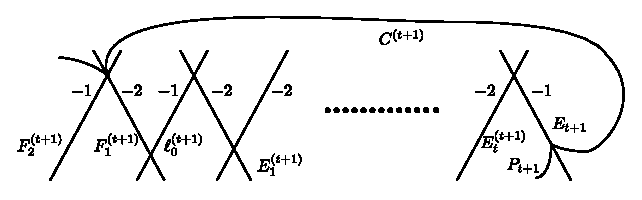
\includegraphics{figures/chap2-fig27.eps}
\end{figure}
\noindent
where\pageoriginale\ $(C^{(t+1)}\cdot F_{2}^{(t+1)})=\nu_{1}$,
$(C^{(t+1)}\cdot F_{1}^{(t+1)})=e_{0}-\nu_{1}$, $(C^{(t+1)}\cdot
E_{t+1})=d_{0}$ and $\mu_{t+1}=\mult_{P_{t+1}}C^{(t+1)}$ with
$e_{0}>\nu_{1}$ and $d_{0}>\mu_{t+1}$. Now let $\tau:V_{t+1}\to V$ be
the contraction of $F^{(t+1)}_{2}$, $\ell^{(t+1)}_{0}$,
$E^{(t+1)}_{1},\ldots,E^{(t+1)}_{t}$, and let
$F_{0}:=\tau(F^{(t+1)}_{1})$, $E_{0}:=\tau(E_{t+1})$,
$\overline{C}:=\tau(C^{(t+1)})$ and
$\overline{\Lambda}:=\tau_{\ast}(\Lambda^{(t+1)})$. Then it is easy to
show the following assertions:
\begin{enumerate}
\renewcommand{\labelenumi}{\rm(\theenumi)}
\item $\overline{\Lambda}$ is spanned by $\overline{C}$ and
  $d_{0}F_{0}+(e_{0}-td_{0})E_{0}$, where $e_{0}>td_{0}$, 

\item $(E^{2}_{0})=0$, $(F^{2}_{0})=t$ and $(E_{0}\cdot F_{0})=1$,

\item $\overline{C}\cdot E_{0}=d_{0}\cdot P_{0}$ and
  $\overline{C}\cdot F_{0}=e_{0}\cdot Q_{0}$, where $P_{0}\not\in
  F_{0}$ and $Q_{0}\not\in E_{0}$,

\item $d_{1}:=\mult_{P_{0}}\overline{C}=\mu_{t+1}<d_{0}$ and
  $e_{1}:=\mult_{Q_{0}}\overline{C}=\nu_{1}<e_{0}$, where
  $e_{0}>d_{0}\geqq e_{1}$ (\cf \ref{chap2:6.8.2}).
\end{enumerate}

\subsection{}\label{chap2:6.9}
In the paragraphs \ref{chap2:6.9} $\sim$ \ref{chap2:6.13} we assume that $d_{0}>1$
and use the notations set forth in the assertions (1) $\sim$ (4) of
\ref{chap2:6.8.4}. Find integers $d_{2},\ldots,d_{m}$ and
$p_{1},\ldots,p_{m}$ by the Euclidea algorithm with respect to $d_{0}$
and $d_{1}$: 
\begin{alignat*}{2}
d_{0} &= p_{1}d_{1}+d_{2}\qquad && 0<d_{2}<d_{1}\\
d_{1} &= p_{2}d_{2}+d_{3}\qquad && 0<d_{3}<d_{2}\\
&\quad\ldots\ldots &\\
d_{m-2} &= p_{m-1}d_{m-1}+d_{m} \qquad && 0<d_{m}<d_{m-1}\\
d_{m-1} &= p_{m}d_{m} \qquad && 1<p_{m}
\end{alignat*}
Similarly, find integers $e_{2},\ldots,e_{n}$ and $q_{1},\ldots,q_{n}$
by the Euclidean algorithm with respect to $e_{0}$ and $e_{1}:$
\begin{alignat*}{2}
e_{0} &= q_{1}e_{1}+e_{2}\qquad && 0<e_{2}<e_{1}\\
e_{1} &= q_{2}e_{2}+e_{3} \qquad && 0<e_{3}<e_{2}\\
 &\quad\ldots\ldots &&\\
e_{n-2} &= q_{n-1}e_{n-1}+e_{n}\qquad && 0<e_{n}<e_{n-1}\\
e_{n-1} &= q_{n}e_{n} \qquad && 1<q_{n}
\end{alignat*}\pageoriginale\ 
As in \ref{chap2:1.4}, define an integer $a(i,j)(1\leqq i\leqq m;1\leqq
j\leqq p_{i})$ inductively as follows:
\begin{alignat*}{2}
a_{0} &= e_{0}-td_{0} &&\\
a(1,j) &= j(a_{0}-d_{1})  && \text{for } 1\leqq j\leqq p_{1}\\
a(2,j) &= a_{0}+j(a(1,p_{1})-d_{2}) &&\text{for } 1\leqq j\leqq
p_{2}\\
&\quad\ldots\ldots &&\\
a(i,j) &= a(i-2,p_{i-2})+j(a(i-1,p_{i-1})-d_{i})\qquad &&\text{for } 1\leqq
j\leqq p_{i}\\
 & &&\text{and } 2\leqq i\leqq m.
\end{alignat*}
Similarly, define an integer $b(i,j)(1\leqq i\leqq n;1\leqq j\leqq
q_{i})$ inductively as follows:
\begin{alignat*}{2}
b_{0}  &= d_{0}  && \\
b(1,j) &= j(b_{0}-e_{1}) && \text{for } 1\leqq j\leqq q_{1}\\
b(2,j) &= b_{0}+j(b(1,q_{1})-e_{2}) && \text{for } 1\leqq j\leqq
q_{2}\\
 &\quad \ldots\ldots && \\
b(i,j) &= b(i-2,q_{i-2})+j(b(i-1,q_{i-1})-e_{i})\qquad &&\text{for }
1\leqq j\leqq q_{i}\\
 & && \text{and } 2\leqq i\leqq n. 
\end{alignat*}
Then we have the following:

\begin{lemma*}
With the notations as above, we have:
$$
a(m,p_{m})d_{m}=d_{0}(a_{0}-d_{1})\quad\text{and}\quad
b(n,q_{n})e_{n}=e_{0}(b_{0}-e_{1}). 
$$
In\pageoriginale\ particular, $a(m,p_{m})\neq 1$ and $b(n,q_{n})\neq 1$.
\end{lemma*}

\begin{proof}
The first equalities are obtained by straightforward computations (\cf
the proof of Lemma \ref{chap2:1.4.1}, (6)). As for the second assertion,
assume that $a(m,p_{m})=1$. Then $d_{m}\geqq d_{0}$, which is absurd
because $d_{0}>d_{1}\geqq d_{m}$. Hence $a(m,p_{m})\neq 1$. Similarly,
$b(n,q_{n})\neq 1$.
\end{proof}

\subsection{}\label{chap2:6.10}
Set $M:p_{1}+\cdots+p_{m}$. Let $P_{0}$, $P_{1},\ldots,P_{M-1}$ be the
points of $\overline{C}$ over $P_{0}$, $P_{i}$ being infinitely near
to $P_{i-1}$ of order one for $1\leqq i\leqq M-1$. Let
$\sigma_{i}:V_{i}\to V_{i-1}$ be the quadratic transformation of
$V_{i-1}$ with center at $P_{i-1}$ for $1\leqq i\leqq m$.\footnote{By
  abuse of (and also for the sake of simplifying) the notations, we
  use these notations though they overlap in part those introduced in
  \ref{chap2:6.8.1} $\sim$ \ref{chap2:6.8.3}.} 
The composition $\rho_{1}=\sigma_{1}\ldots\sigma_{M}:V_{M}\to
V_{0}:=V$ is called {\em the Euclidean transformation with respect to}
$(\overline{C},P_{0})$ (\cf \ref{chap2:1.3.1}). Let $\rho_{2}:V_{M+N}\to
V_{M}$ be the Euclidean transformation with respect to
$(\rho'_{1}(\overline{C}),\rho^{-1}_{1}(Q_{0}))$, where
$N=q_{1}+\cdots+q_{n}$. Let $W:=V_{M+N}$ and let
$\rho:=\rho_{1}\rho_{2}:W\to V$ be the composition of $\rho_{1}$ and
$\rho_{2}$. Let $C':=\rho'(\overline{C})$ and
$\Lambda':=\rho'(\overline{\Lambda})$. By abuse of notations, we
denote $\rho'(E_{0})$ and $\rho'(F_{0})$ by $E_{0}$ and $F_{0}$ again,
respectively. Then it is by a straightforward computation that we
obtain the following weighted graph of $\rho^{-1}(E_{0}\cup F_{0})$:
\begin{figure}[H]
\centering
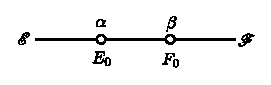
\includegraphics[scale=1.1]{figures/chap2-fig28.eps}
\end{figure}
\noindent
where $\mathscr{E}$ and $\mathscr{F}$ are the graphs similar to that
in the Figure $1$ of \ref{chap2:1.3.4} and where $\alpha=-(p_{1}+1)$ if
$m>1$ and $\alpha=-p_{1}$ if $m=1$,
\begin{figure}[H]
\centerline{{\bf Figure 2~: The weighted graph {\boldmath$\mathscr{E}$}}}

\bigskip
\centering
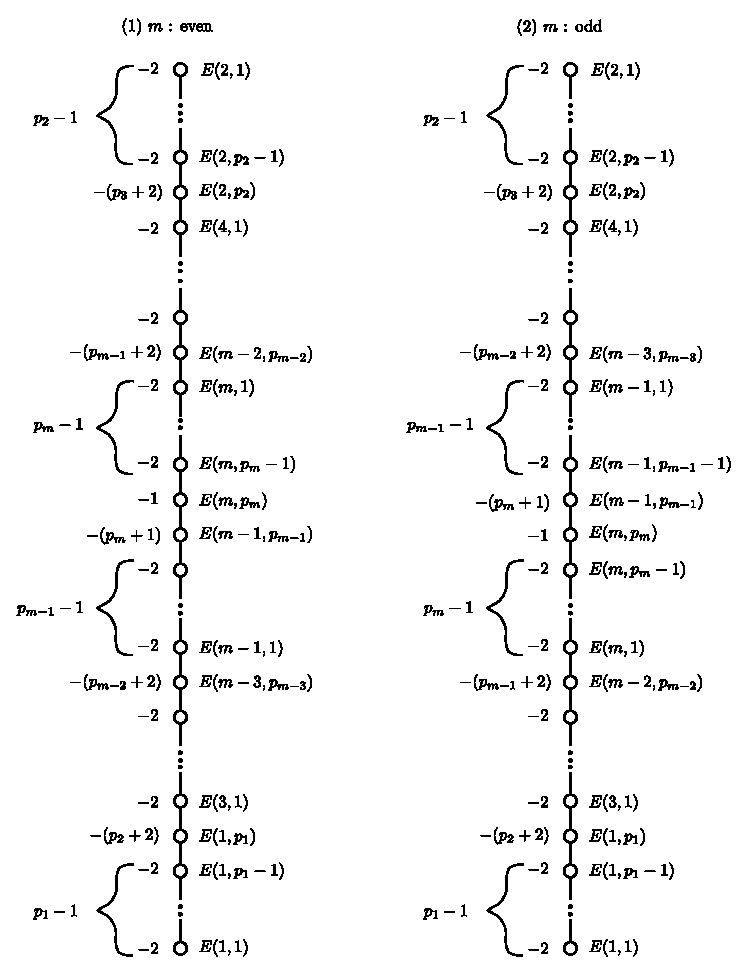
\includegraphics[scale=.9]{figures/chap2-fig29.eps}
\end{figure}\pageoriginale\
\noindent
where $E(2,1)$ is linked to $E_{0}$, $C'$ intersects $E(m,p_{m})$ but
not other components, and $(C'\cdot E(m,p_{m}))=d_{m}$.
\begin{figure}[H]
\centerline{{\bf Figure 3~: The weighted graph {\boldmath$\mathscr{F}$}}}

\bigskip
\centering
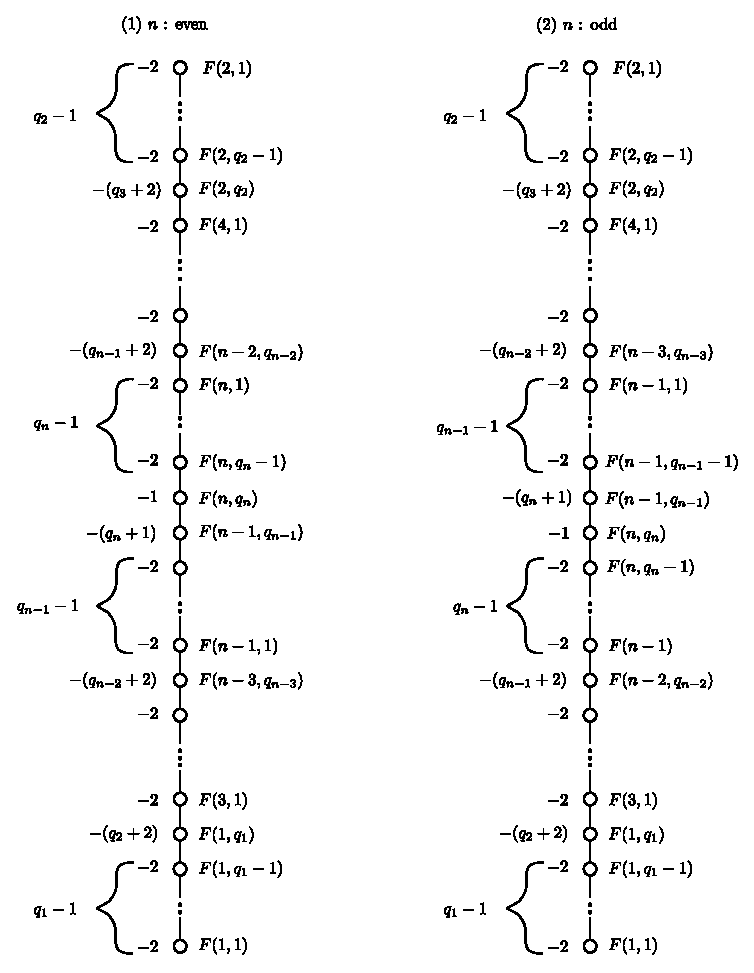
\includegraphics[scale=.9]{figures/chap2-fig30.eps}
\end{figure}\pageoriginale\
\noindent
where $F(2,1)$ is linked to $F_{0}$, $C'$ intersects $F(n,q_{n})$ but
not other components, and $(C'\cdot
F(n,q_{n}))=e_{n}$. $\beta=t-(q_{1}+1)$\pageoriginale\ if $n>1$ and
$\beta=t-q_{1}$ if $n=1$. In order to keep the notations in accordance
with the present ones, we shall write down the graphs $\mathscr{E}$
and $\mathscr{F}$ in the Figures 2 and 3, which are given in the next
two pages.

\subsection{}\label{chap2:6.11}
With the notations of \ref{chap2:6.9} and \ref{chap2:6.10}, we have the following:

\begin{lemma*}
\begin{enumerate}
\renewcommand{\labelenumi}{\rm(\theenumi)}
\item The linear pencil $\Lambda'$ is spanned by $C'$ and 
$$
\Delta':=a_{0}E_{0}+b_{0}F_{0}+\sum^{m}_{i=1}\sum^{p_{i}}_{j=1}a(i,j)E(i,j)+\sum^{n}_{i=1}\sum^{q_{i}}_{j=1}b(i,j)F(i,j) 
$$

\item $a_{0}>0$ and $a(i,j)\geqq 0$ for $1\leqq i\leqq m$ and $1\leqq
  j\leqq p_{i}$; moreover, if $E(i,j)$ lies between $E_{0}$ and
  $E(m,p_{m})$ (excluding $E(m,p_{m})$) in the graph $\mathscr{E}$
  then the multiplicity $a(i,j)>0$.

\item $b_{0}>0$ and $b(i,j)\geqq 0$ for $1\leqq i\leqq n$ and $1\leqq
  j\leqq q_{i}$; moreover, if $F(i,j)$ lies between $F_{0}$ and
  $F(n,q_{n})$ (excluding $F(n,q_{n})$) in the graph $\mathscr{F}$
  then the multiplicity $b(i,j)>0$.
\end{enumerate}
\end{lemma*}

\begin{proof}
\begin{enumerate}
\renewcommand{\labelenumi}{(\theenumi)}
\item By a straightforward computation we obtain $C'\sim \Delta'$. By
  the assumption at the beginning of \ref{chap2:6.8.2}, $C'$ is an
  irreducible member of $\Lambda'$. Hence the assertion (1) holds.

\item Since $\Lambda'$ consists of effective divisors we know that
  $a(i,j)\geqq 0$ for $1\leqq i\leqq m$ and $1\leqq j\leqq
  p_{i}$. Besides, $a_{0}=e_{0}-td_{0}>0$ (\cf \ref{chap2:6.8.3}). If
  $E(i,j)\neq E(m,p_{m})$, then $(C'\cdot E(i,j))=0$, which implies
  that $E(i,j)$ is an irreducible component of a member of
  $\Lambda'$. Especially, if $E(i,j)$ lies between $E_{0}$ and
  $E(m,p_{m})$ in the graph $\mathscr{E}$, it is readily seen that
  $E(i,j)$ is connected to $E_{0}$ through the components of
  $\Delta'$. Hence $E(i,j)$ is a component of $\Delta'$, \iec
  $a(i,j)>0$.

\item The\pageoriginale\ assertion (3) is proved by the same argument
  as above. 
\end{enumerate}
\end{proof}

\subsection{}\label{chap2:6.12}
\begin{lemma*}
  \begin{enumerate}
    \renewcommand{\labelenumi}{\rm(\theenumi)}
  \item Assume that $a(1,1)=0$. Then $a(m,p_{m})=0$ and $a(i,j)=0$
    whenever $E(i,j)$ lies between $E(1,1)$ and $E(m,p_{m})$ in the
    graph $\mathscr{E}$; such $E(i,j)$'s with $a(i,j)=0$ (excluding
    $E(m,p_{m})$) are contained in one and only one member of
    $\Lambda'$; $E(m,p_{m})$ is a cross-section of $\Lambda'$, esp.\@ $d_{m}=1$.
    
  \item Assume that $b(1,1)=0$. Then $b(n,q_{n})=0$ and $b(i,j)=0$
    whenever $F(i,j)$ lies between $F(1,1)$ and $F(n,q_{n})$ in the
    graph $\mathscr{F}$; such $F(i,j)$'s with $b(i,j)=0$ (excluding
    $F(n,q_{n})$) are contained in one and only one member of
    $\Lambda'$; $F(n,q_{n})$ is a cross-section of $\Lambda'$, esp.\@ $e_{n}=1$.
  \end{enumerate}
\end{lemma*}

\begin{proof}
We shall prove only the assertion (1) because the assertion (2) is
proved in a similar fashion. The assumption $a(1,1)=0$ implies that
$a(m,p_{m})=0$ (\cf Lemma \ref{chap2:6.9}) and that $E(1,1)$ is contained
in a member of $\Lambda'$ other than $\Delta'$ (and $C'$, of
course). If $E(i,j)$ $(\neq E(m,p_{m}))$ lies between $E(1,1)$ and
$E(m,p_{m})$ in the graph $\mathscr{E}$ then it is readily seen that
$E(i,j)$ is contained in the same member of $\Lambda'$ as $E(1,1)$ is,
which implies $a(i,j)=0$. Moreover, we know that $E(m,p_{m})$ is a
quasi-section of $\Lambda'$. Since $(C'\cdot E(m,p_{m}))=d_{m}$ and
every member of $\Lambda'$ has a one-place point on $E(m,p_{m})$, we
know that $d_{m}=1$.
\end{proof}

\subsection{}\label{chap2:6.13}
We shall prove the following:

\begin{lemma*}
With the notations as above, we have:
\begin{enumerate}
\renewcommand{\labelenumi}{\rm(\theenumi)}
\item $a(1,1)=b(1,1)=0$,\pageoriginale\

\item $d_{0}=e_{1}$, $d_{1}=e_{2}$, $n=m+1$ and $(d_{0},e_{0})=1$.
\end{enumerate}
\end{lemma*}

\begin{proof}
Our proof consists of four subparagraphs \ref{chap2:6.13.1} $\sim$ \ref{chap2:6.13.4}.
\end{proof}

\subsubsection{}\label{chap2:6.13.1}
Assume that $a(1,1)>0$ and $b(1,1)>0$. Then it is clear from the
arguments in the previous paragraphs that the following assertions
hold true:
\begin{enumerate}
\renewcommand{\labelenumi}{\theenumi$^{\circ}$}
\item $a(i,j)>0$ for every pair $(i,j)$ with $1\leqq i\leqq m$ and
  $1\leqq j\leqq p_{i}$; similarly, $b(i,j)>0$ for every pair $(i,j)$
  with $1\leqq i\leqq n$ and $1\leqq j\leqq q_{i}$,

\item $a(m,p_{m})\neq 1$ and $b(n,q_{n})\neq 1$ (\cf Lemma
  \ref{chap2:6.9}),

\item the set $B'$ of base points of the pencil $\Lambda'$ consists of
  two points $P'$ and $Q'$ lying on $E(m,p_{m})$ and $F(n,q_{n})$,
  respectively, such that $P'\not\in$ the components of $\Delta'$
  other than $E(m,p_{m})$ and $Q'\not\in$ the components of $\Delta'$
  other than $F(n,q_{n})$,

\item all components of $\Delta'$ except $E(m,p_{m})$, $F(n,q_{n})$
  and $F_{0}$ have self-intersection multiplicities $\leqq -2$.
\end{enumerate}

Since $\Lambda'$ is a linear pencil of rational curves as assumed,
Lemma \ref{chap2:2.3}, (4) implies that $\beta=-1$, \iec $F_{0}$ is
contractible. Let $\tau_{1}:W\to W_{1}$ be the contraction of the
components $F_{0}$, $F(2,1),\ldots,F(2,q_{2}-1)$. Then
$(\tau_{1}(E_{0})^{2})=\alpha+q_{2}$ and
$((\tau_{1}F(2,q_{2}))^{2})=-(q_{3}+1)\leqq -2$; a unique contractible
component of $\tau_{1^{\ast}}(\Delta')$ is $\tau_{1}(E_{0})$, \iec
$\alpha+q_{2}=-1$. Let $\tau_{2}:W_{1}\to W_{2}$ be the contraction of
$\tau_{1}(E_{0})$,
$\tau_{1}(E(2,1)),\ldots,\tau_{1}(E(2,p_{2}-1))$. Then
$((\tau_{2}\tau_{1}F(2,q_{2}))^{2})=-(q_{3}-p_{2}+1)$ and
$((\tau_{2}\tau_{1}E(2,p_{2}))^{2})=-(p_{3}+1)$; a unique contractible
component of $(\tau_{2}\tau_{1})_{\ast}\Delta'$ is
$\tau_{2}\tau_{1}F(2,q_{2})$. We repeat the contractions of this
kind\pageoriginale\ as far as we can. Let $\tau:W\to Z$ be the
contraction of all possible components of $\Delta'$ lying between
$E(m,p_{m})$ and $F(n,q_{n})$ of the weighted graph of $\Delta'$
(excluding $E(m,p_{m})$ and $F(n,q_{n})$). Then the pencil
$\tau_{\ast}\Lambda'$ (= the proper transform of $\Lambda'$ by
$\tau$), which is spanned by $\tau(C')$ and $\tau_{\ast}\Delta'$,
satisfies the same properties as the pencil observed in \ref{chap2:6.4}.

\subsubsection{}\label{chap2:6.13.2}
Set $D_{1}:=\tau(E(m,p_{m}))$, $D_{2}:=\tau(F(n,q_{n}))$,
$p:=(D^{2}_{1})$ and $q:=(D^{2}_{2})$. Write the weighted graph of
$\tau_{\ast}(\Delta')$ in the form:
\begin{figure}[H]
\centering
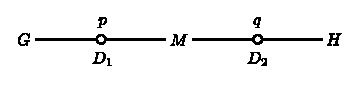
\includegraphics[scale=1.1]{figures/chap2-fig31.eps}
\end{figure}
\noindent
where:
\begin{enumerate}
\renewcommand{\labelenumi}{\theenumi$^{\circ}$}
\item $G$ coincides with the subgraph of $\mathscr{E}$ between
  $E(1,1)$ and $E(m,p_{m})$ (excluding $E(m,p_{m})$); hence $G\neq \phi$,

\item $H$ coincides with the subgraph of $\mathscr{F}$ between
  $F(1,1)$ and $F(n,q_{n})$ (excluding $F(n,q_{n})$); hence $H\neq
  \phi$,

\item $M$ is the weighted graph of the images by $\tau$ of the
  components of $\Delta'$ which lie between $E(m,p_{m})$ and
  $F(n,q_{n})$ in the weighted graph of $\Delta'$ (excluding
  $E(m,p_{m})$ and $F(n,q_{n})$); $M$ might be empty,

\item either $p\leqq 0$ or $q\leqq 0$.
\end{enumerate}
Only the assertion $4^{\circ}$ needs a proof. Assume that $p>0$ and
$q>0$. Then $M=\phi$. However, by the contraction $\tau$, either the
component of $\Delta'$ next to $E(m,p_{m})$ and not belonging to $G$
(\iec $E(m,p_{m}-1)$ if $m$ is even; $E(m-1,p_{m-1})$ if $m$ is odd
and $m>1$; $E_{0}$ if $m=1$) or\pageoriginale\ the component of
$\Delta'$ next to $F(n,q_{n})$ and not belonging to $H$ (\iec
$F(n,q_{n}-1)$ if $n$ is even; $F(n-1,q_{n-1})$ if $n$ is odd and
$n>1$; $F_{0}$ if $n=1$) is contracted last. Then $p=0$ or $q=0$,
which is a contradiction. Hence either $p\leqq 0$ or $q\leqq 0$. Now,
noting that $a(m,p_{m})\neq 1$ and $b(n,q_{n})\neq 1$ (\cf
\ref{chap2:6.13.1}, $2^{\circ}$), we know by Lemma \ref{chap2:6.5} that either
$G=\phi$ or $H=\phi$. This is a contradiction. Therefore we have
either $a(1,1)=0$ or $b(1,1)=0$.


\subsubsection{}\label{chap2:6.13.3}
Assume that $a(1,1)=0$ and $b(1,1)>0$. Then the following assertions
hold true:
\begin{enumerate}
\renewcommand{\labelenumi}{\theenumi$^{\circ}$}
\item $a(i,j)>0$ if $E(i,j)$ lies between $E_{0}$ and $E(m,p_{m})$
  (excluding $E(m,p_{m})$) in the graph $\mathscr{E}$ and $a(i,j)=0$
  if otherwise; $b(i,j)>0$ for every pair $(i,j)$ with $1\leqq i\leqq
  n$ and $1\leqq j\leqq q_{i}$,

\item set $D_{1}:=F_{0}$, $D_{2}:=F(n,q_{n})$, $p:=\beta=(D^{2}_{1})$
  and $q=-1=(D^{2}_{2})$; then $\Delta'$ has the following weighted
  graph:
\begin{figure}[H]
\centering
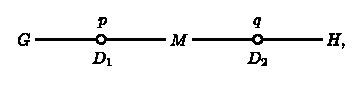
\includegraphics[scale=1.1]{figures/chap2-fig32.eps}
\end{figure}
\noindent
where: 
\begin{enumerate}
\renewcommand{\theenumii}{\roman{enumii}}
\renewcommand{\labelenumii}{\rm(\theenumii)}
\item $G$ is the weighted graph consisting of $E_{0}$ and
components of $\mathscr{E}$ lying between $E_{0}$ and $E(m,p_{m})$
(excluding $E(m,p_{m})$), 

\item $M$ coincides with the subgraph of $\mathscr{F}$ between $F_{0}$
  and \break $F(n,q_{n})$ (excluding $F(n,q_{n})$),

\item $H$ coincides with the subgraph of $\mathscr{F}$ between
  $F(1,1)$ and $F(n,q_{n})$ (excluding $F(n,q_{n})$); hence $H\neq \phi$;
\end{enumerate}

\item the set $B'$ of base points of $\Lambda'$ consists of a single
  point $Q'$ on $D_{2}$ but not on the other components of $\Delta'$,

\item $b(n,q_{n})\neq 1$\pageoriginale\ (\cf \ref{chap2:6.13.1},
  $2^{\circ}$),

\item the multiplicity $a(m,p_{m}-1)=d_{m}=1$ if $m$ is even;
  $a(m-1,p_{m-1})=d_{m}=1$ if $m$ is odd and $m>1$; $a_{0}=d_{1}=1$ if
  $m=1$ (\cf Lemma \ref{chap2:6.12}, (1)).
\end{enumerate}

We shall apply Lemma \ref{chap2:6.6} to the present situation. First, we
know that $p=-1$, \iec $t=q_{1}$, because $q=-1$ (\cf Lemma
\ref{chap2:6.6}, (1) or (2)). Since $H\neq \phi$ and $b(n,q_{n})\neq 1$,
Lemma \ref{chap2:6.6}, (3) implies that any component in the graphs $G$
and $M$ as well as $D_{1}$ has multiplicity $>1$ in $\Delta'$. However
this contradicts the assertion $5^{\circ}$ above.

Therefore, the case where $a(1,1)=0$ and $b(1,1)>0$ does not
occur. Similarly, we can show that the case where $a(1,1)>0$ and
$b(1,1)=0$ does not occur.

\subsubsection{}\label{chap2:6.13.4}
We have thus proved that $a(1,1)=b(1,1)=0$. Hence $\Lambda'$ has no
base points, and $E(m,p_{m})$ and $F(n,q_{n})$ are cross-sections of
$\Lambda'$, \iec $d_{m}=e_{n}=1$. By definition of $a(1,1)$ and
$b(1,1)$ (\cf \ref{chap2:6.9}), the equalities $a(1,1)=b(1,1)=0$ imply that
$e_{0}=td_{0}+d_{1}$ and $d_{0}=e_{1}$, where $t=q_{1}$ if $n>1$ and
$t=q_{1}-1$ if $n=1$\footnote{Since $F_{0}$ must be an exceptional
  component of $\Delta'$ we have $\beta=-1$.}. If $n=1$ and
$t=q_{1}-1$ then $d_{1}=e_{1}=d_{0}$, which is a contradiction as
$d_{0}>d_{1}$. Hence, $n>1$ and $t=q_{1}$. Then, since
$e_{0}=q_{1}e_{1}+d_{1}$, we have $d_{1}=e_{2}$. This implies that
$n=m+1$, $d_{0}=e_{1}$, $d_{1}=e_{2},\ldots,d_{m}=e_{n}$, and
$p_{1}=q_{2},\ldots,p_{m}=q_{n}$. In particular,
$(d_{0},e_{0})=e_{n}=1$. This completes a proof of Lemma \ref{chap2:6.13}.

\subsection{}\label{chap2:6.14}
Returning to the situation of \ref{chap2:6.8.1}, we shall assume in this
paragraph that $d_{0}=1$. Let $\tau:V_{1}\to V$ be the contraction of
$\ell^{(1)}_{0}$, and let $E_{0}:=\tau(E_{1})$, $F_{0}:=\tau(F_{1})$,
$\overline{C}:=\tau(C^{(1)})$ and
$\overline{\Lambda}:=\tau_{\ast}(\sigma'_{1}\Lambda)$. Then\pageoriginale\
we have:
\begin{enumerate}
\renewcommand{\labelenumi}{(\theenumi)}
\item $\overline{\Lambda}$ is spanned by $\overline{C}$ and
  $e_{0}E_{0}+F_{0}$,

\item $(E^{2}_{0})=(F^{2}_{0})=0$ and $(E_{0}\cdot F_{0})=1$; thence
  $V$ is isomorphic to $\mathbb{P}^{1}_{k}\times \mathbb{P}^{1}_{k}$
  whose two distinct fibrations by $\mathbb{P}^{1}_{k}$ are given by
  the linear pencils $|E_{0}|$ and $|F_{0}|$,

\item $\overline{C}\cdot E_{0}=P_{0}$ and $\overline{C}\cdot
  F_{0}=e_{0}\cdot Q_{0}$, where $P_{0}$, $Q_{0}\neq E_{0}F_{0}$.
\end{enumerate}

We shall show the following:

\begin{lemma*}
\begin{enumerate}
\setcounter{enumi}{3}
\renewcommand{\labelenumi}{\rm(\theenumi)}
\item $\overline{C}$ is nonsingular.

\item Let $\rho:W\to V$ be the shortest composition of quadratic
  transformations by which the proper transform
  $\Lambda':=\rho'(\overline{\Lambda})$ of $\overline{\Lambda}$ by
  $\rho$ has no base points. Then we have:
\begin{enumerate}
\renewcommand{\theenumii}{\roman{enumii}}
\renewcommand{\labelenumii}{\rm(\theenumii)}
\item $\rho^{-1}(E_{0}\cup F_{0})$ has the following weighted graph:
\begin{figure}[H]
\centering
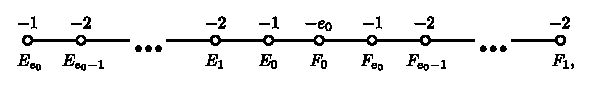
\includegraphics[scale=1.1]{figures/chap2-fig33.eps}
\end{figure}
\noindent
where, by abuse of notations, we denote $\rho'(E_{0})$ and
$\rho'(F_{0})$ by $E_{0}$ and $F_{0}$, respectively,

\item $\Lambda'$ is spanned by $C':=\rho'(\overline{C})$ and
  $\Delta':={\displaystyle{\mathop{\sum}^{e_{0}-1}}_{i=0}}(e_{0}-i)E_{i}+F_{0}$, 

\item $E_{e_{0}}$ and $F_{e_{0}}$ are cross-sections of $\Lambda'$,

\item $F_{1},\ldots,F_{e_{0}-1}$ are contained in one and only one
  member of $\Lambda'$.
\end{enumerate}
\end{enumerate}
\end{lemma*}

\begin{proof}
\begin{enumerate}
\setcounter{enumi}{3}
\renewcommand{\labelenumi}{\rm(\theenumi)}
\item Let $E$ be a member of $|E_{0}|$ such that $Q_{0}\in
  E_{0}$. Then, since $E_{0}$ is isomorphic to $\mathbb{P}^{1}_{k}$
  and $(\overline{C}\cdot E)=1$, $\overline{C}$ is non-singular at
  $Q_{0}$. $\overline{C}$ is apparently nonsingular at other points.

\item follows from a straightforward computation.
\end{enumerate}
\end{proof}

\subsection{}\label{chap2:6.15}
Let\pageoriginale\ $W$, $\Lambda'$, $C'$ and $\Delta'$ be as in
\ref{chap2:6.10} (and \ref{chap2:6.11}) or \ref{chap2:6.14}. Since $\Lambda'$ has no
base points, $\Lambda'$ defines a surjective morphism $\varphi:W\to
\mathbb{P}^{1}_{k}$ whose fibers are members of $\Lambda'$. Set
$S_{1}:=E(m,p_{m})$ and $S_{2}:=F(n,q_{n})$ if $d_{0}>1$; set
$S_{1}:=E_{e_{0}}$ and $S_{2}:=F_{e_{0}}$ if $d_{0}=1$. Then both
$S_{1}$ and $S_{2}$ are cross-sections (\cf Lemmas \ref{chap2:6.12} and
\ref{chap2:6.14}). When $d_{0}>1$, let $R_{1}$ be the union of $E(i,j)$'s
which lie between $E(1,1)$ and $E(m,p_{m})$ in the graph $\mathscr{E}$
(with $F(1,1)$ included and $E(m,p_{m})$ excluded), and let $R_{2}$ be
the union of $F(i,j)$'s which lie between $F(1,1)$ and $F(n,q_{n})$ in
the graph $\mathscr{F}$ (with $F(1,1)$ included and $F(n,q_{n})$
excluded). Note that $R_{1}\neq \phi$ and $R_{2}\neq \phi$. When
$d_{0}=1$ and $e_{0}>1$, let $R$ be the union of
$F_{1},\ldots,F_{e_{0}-1}$. Let $\Gamma_{1}$ and $\Gamma_{2}$ be the
fibers of $\varphi$ containing $R_{1}$ and $R_{2}$, respectively if
$d_{0}>1$; let $\Gamma$ be the fiber of $\varphi$ containing $R$ if
$d_{0}=1$ and $e_{0}>1$. Set $U:=W-(R_{1}\cup R_{2}\cup S_{1}\cup
S_{2}\cup \Supp(\Delta'))$ if $d_{0}>1$; set $U:=W-(R\cup S_{1}\cup
S_{2}\cup \Supp(\Delta'))$ if $d_{0}=1$ and $e_{0}>1$; set
$U:=W-(S_{1}\cup S_{2}\cup\Supp(\Delta'))$ if $d_{0}=e_{0}=1$. Then
$U$ is isomorphic to the affine plane $\mathbb{A}^{2}_{k}$. We shall
prove the next:

\begin{lemma*}
With the above notations, we have:
\begin{enumerate}
\setcounter{enumi}{3}
\renewcommand{\labelenumi}{\rm(\theenumi)}
\item If $d_{0}>1$ then $\Gamma_{1}=\Gamma_{2}$; we set
  $\Gamma:=\Gamma_{1}=\Gamma_{2}$. 

\item If either $d_{0}>1$ or $d_{0}=1$ and $e_{0}>1$ then $\Gamma$ has
  exactly two irreducible components $C_{1}$ and $C_{2}$ other than
  those contained in $R_{1}$ or $R_{2}$ (or $R$ if $d_{0}=1$ and
  $e_{0}>1$).

\item If $d_{0}=e_{0}=1$, the fibration $\varphi$ has only one
  reducible fiber $\Gamma$ which has two irreducible components.
\end{enumerate}
\end{lemma*}

\begin{proof}
Our\pageoriginale\ proof consists of four steps.
\begin{enumerate}
\renewcommand{\theenumi}{\Roman{enumi}}
\renewcommand{\labelenumi}{\rm(\theenumi)}
\item We shall prove first the following assertion:
\end{enumerate}
\end{proof}

{\em The fibration $\varphi$ has one and only one fiber
  $\varphi^{-1}(Q)$ $(Q\in \mathbb{P}^{1}_{k})$ such that
  $\varphi^{-1}(Q)\cap U$ is reducible; then $\varphi^{-1}(Q)\cap U$
  consists of two irreducible components.}

\begin{proof}
Let $Q_{1},\ldots,Q_{s}$ be the points of $\mathbb{P}^{1}_{k}$ such
that $\varphi^{-1}(Q_{i})\cap U$ is reducible for $1\leqq i\leqq s$,
and let $Q_{s+1},\ldots,Q_{t}$ be the points of $\mathbb{P}^{1}_{k}$
such that $\varphi^{-1}(Q_{i})$ is reducible but
$\varphi^{-1}(Q_{i})\cap U$ is irreducible for $s+1\leqq i\leqq t$. We
may assume that $\varphi^{-1}(Q_{1}),\ldots,\varphi^{-1}(Q_{s})$ and
$\varphi^{-1}(Q_{s+1}),\ldots,\varphi^{-1}(Q_{t})$ exhaust all fibers
of $\varphi$ having respective properties. Then
$\varphi^{-1}(Q_{i})$'s $(1\leqq i\leqq t)$ and
$\varphi^{-1}(Q_{\infty}):=\Delta'$ are all reducible fibers of
$\varphi$. For $1\leqq i\leqq s$, let $n_{i}$ be the number of
irreducible components of $\varphi^{-1}(Q_{i})\cap U$. On the other
hand, write $U:=\Spec(A)$ and
$U-\left({\displaystyle{\mathop{\bigcup}^{t}_{i=1}}}\varphi^{-1}(Q_{i})\cap
U\right):=\Spec(B)$. Then, since $U$ is isomorphic to $\mathbb{A}^{2}_{k}$,
we know that $A$ is a unique factorization domain and
$A^{\ast}=k^{\ast}$. Hence, by a similar argument as in
(\ref{chap1:2.3.3}), we know that $B^{\ast}/k^{\ast}$ is a free $z$-module
of rank $n_{1}+\cdots+n_{s}+(t-s)$. Since
$\varphi^{-1} (\mathbb{P}^{1}_{k}-\{Q_{1},\ldots,Q_{t},Q_{\infty}\})$
is a $\mathbb{P}^{1}$-bundle over
$\mathbb{P}^{1}_{k}-\{Q_{1},\ldots,Q_{t},Q_{\infty}\}$ and
$U-\left({\displaystyle{\mathop{\bigcup}^{t}_{i=1}}}\varphi^{-1}(Q_{i})\cap
U\right) =\varphi^{-1}(\mathbb{P}^{1}_{k}-\{Q_{1}, \ldots,
Q_{t},Q_{\infty}\})-(S_{1}\cup  
S_{2})$, we know that
$U-({\displaystyle{\mathop{\bigcup}^{t}_{i=1}}}\varphi^{-1}(Q_{i})\cap
U)$ is isomorphic to
$\mathbb{A}^{1}_{\ast}\times(\mathbb{P}^{1}_{k}\{Q_{1},\ldots,Q_{t},Q_{\infty}\})$,
where $\mathbb{A}^{1}_{\ast}=\mathbb{A}^{1}_{k}$-(one point). Then by
virtue of the unit theorem (\cf Sweedler \cite{54}),
$B^{\ast}/k^{\ast}$ is a free $z$-module of rank $1+t$. Hence we
obtain
$$
n_{1}+\cdots+n_{s}+(t-s)=1+t,\quad n_{i}\geqq 2(1\leqq i\leqq s)
$$
whence\pageoriginale\ follows that $s=1$ and $n_{1}=2$.

\begin{enumerate}
\renewcommand{\theenumi}{\Roman{enumi}}
\renewcommand{\labelenumi}{\rm(\theenumi)}
\setcounter{enumi}{1}
\item Assume that $d_{0}>1$ and $\Gamma_{1}\neq \Gamma_{2}$. Then,
  each of $\Gamma_{1}$ and $\Gamma_{2}$ has two irreducible components
  other than those contained in $R_{1}$ and $R_{2}$. Suppose that
  $\Gamma_{1}$ has only one irreducible component $C_{1}$ other than
  those contained in $R_{1}$. Then the multiplicity of $C_{1}$ in
  $\Gamma_{1}$ is $1$ and $(C_{1}\cdot S_{2})=1$. Since the components
  of $\Gamma_{1}$ contained in $R_{1}$ are not exceptional components,
  Lemma \ref{chap2:2.2} tells us that not only $C_{1}$ is an exceptional
  component of $\Gamma_{1}$ but also $\Gamma_{1}$ contains another
  exceptional component. This is a contradiction. Therefore, we know
  that $\Gamma_{1}\cap U$ and $\Gamma_{2}\cap U$ are reducible. But
  this contradicts the assertion proved in the step (I) above. Hence
  $\Gamma_{1}=\Gamma_{2}$. By the same argument, we can show that
  $\Gamma$ has two irreducible components $C_{1}$ and $C_{2}$ other
  than those contained in $R$ provided $d_{0}=1$ and $e_{0}>1$.

\item We shall show that if $d_{0}>1$ then
  $\Gamma(:=\Gamma_{1}=\Gamma_{2})$ has two irreducible components
  $C_{1}$ and $C_{2}$ other than those contained in $R_{1}$ or
  $R_{2}$. Assume the contrary, \iec $\Gamma\cap U$ in
  irreducible. Then, the assertion proved in the step (I) implies that
  there exists a reducible fiber $\varphi^{-1}(Q)$ of the form:
    $\varphi^{-1}(Q)=L_{1}+L_{2}$, where $L_{1}\cong
    L_{2}\cong\mathbb{P}^{1}_{k}$, $(L_{1}\cdot L_{2})=(L_{1}\cdot
    S_{1})=(L_{2}\cdot S_{2})=1$, $(L_{1}\cdot S_{2})=(L_{2}\cdot
    S_{1})=0$ and $(L^{2}_{1})=(L^{2}_{2})=-1$. Then $L_{1}\cap U$ and
    $L_{2}\cap U$ are isomorphic to the affine line
    $\mathbb{A}^{1}_{k}$; moreover, they satisfy the conditions (1)
    $\sim$ (5) of Theorem \ref{chap2:3.2}, Chapter I. Hence, after a
    suitable change of coordinates $x$, $y$ of $U:\Spec(k[x,y])$, we
    may assume that $L_{1}\cap U$ and $L_{2}\cap U$ are the $x$-axis
    and the $y$-axis, respectively; namely, $\varphi^{-1}(Q)\cap
    U$\pageoriginale\ is defined by $xy=0$. Then $\fprod{\Gamma}{U}{W}$
    (with scheme structure) is isomorphic to $\Spec(k[x,y]/(xy-c))$
    for $c\in k^{\ast}$, which is reduced. However, we shall show that
    $\fprod{\Gamma}{U}{W}$ is not reduced. Indeed, let $C_{1}$ be the
    unique irreducible component of $\Gamma$ which is not contained in
    $R_{1}$ and $R_{2}$. Then, since the components in $R_{1}$ and
    $R_{2}$ are not exceptional components, $C_{1}$ must be an
    exceptional component of $\Gamma$. Then the multiplicity of
    $C_{1}$ in $\Gamma$ is larger than $1$ because $R_{1}\neq \phi$,
    $R_{2}\neq \phi$ and $C_{1}$ connects $R_{1}$ to $R_{2}$. Thus, we
    get a contradiction, and proved that $\Gamma$ has two irreducible
    components $C_{1}$ and $C_{2}$ other than those contained in
    $R_{1}$ or $R_{2}$.

\item If $d_{0}=e_{0}=1$, the assertion proved in the step (I) implies
  that there exists a fiber $\varphi^{-1}(Q)=L_{1}+L_{2}$ such that
  $L_{1}\cong L_{2}\cong \mathbb{P}^{1}_{k}$, $(L_{1}\cdot
  L_{2})=(L_{1}\cdot S_{1})=(L_{2}\cdot S_{2})=1$, $(L_{1}\cdot
  S_{2})=(L_{2}\cdot S_{1})=0$ and $(L^{2}_{1})=(L^{2}_{2})=-1$.
\end{enumerate}
\end{proof}

\subsection{}\label{chap2:6.16}
In this paragraph we shall derive a consequence of Lemma
\ref{chap2:6.15}, which also completes a proof of the ``if'' part of
Theorem \ref{chap2:6.1}.

\begin{lemma*}
Let $f$ be an irreducible element of $k[x,y]$ satisfying the
conditions $(1)$, $(2)$ and $(3)$ of Theorem \ref{chap2:6.1}. Then $f$ is
written in the form $f=c(x^{d}y^{e}-1)$ after a suitable change of
coordinates $x$, $y$ of $k[x,y]$, where $c\in k^{\ast}$, and $d$ and
$e$ are positive integers such that $(d,e)=1$.
\end{lemma*}

\begin{proof}
With the notations of \ref{chap2:6.15}, let $\Gamma$ be the unique fiber of
$\varphi$ such that $\Gamma\cap U$ is reducible; as a matter of fact,
$\Gamma\cap U$ consists of two irreducible components. Let $C_{1}$ and
$C_{2}$ be irreducible\pageoriginale\ components of $\Gamma$ such that
$C_{i}\cap U\neq \phi$ for $i=1,2$, and let $d$ and $e$ be
multiplicities of $C_{1}$ and $C_{2}$ in $\Gamma$, respectively. Since
$\Gamma\cap U$ is connected $C_{1}$ and $C_{2}$ intersect each other
transversely in a single point on $U$. Furthermore, $C_{1}\cap U$ and
$C_{2}\cap U$ are isomorphic to the affine line. We shall show the
latter assertion only in the case $d_{0}>1$ as the remaining cases
($d_{0}=1$ and $e_{0}>1$; $d_{0}=e_{0}=1$) can be treated in a similar
fashion. Since $R_{1}\neq \phi$ and $R_{1}\cap R_{2}=\phi$, either one
of $C_{1}$ and $C_{2}$, say $C_{1}$, intersects a component in
$R_{1}$. Then $C_{2}\cap R_{1}=\phi$, for otherwise $C_{1}\cup
C_{2}\cup R_{1}$ would contain a cyclic chain. The same reasoning
implies that $C_{2}\cap R_{2}=\phi$ if $C_{1}\cap R_{2}\neq
\phi$. Hence, if $C_{1}\cap R_{2}\neq \phi$ then $C_{2}\cap
R_{i}=\phi$ for $i=1,2$, \iec $C_{2}\subset U$, which is absurd as $U$
is affine. Thus $C_{1}\cap R_{2}=\phi$ and $C_{2}\cap R_{2}\neq
\phi$. Moreover, $C_{i}$ intersects $R_{i}$ in a single point for
$i=1,2$, for otherwise $C_{i}\cup R_{i}$ would contain a cyclic
chain. Since $C_{i}\cong \mathbb{P}^{1}_{k}$, we finally know that
$C_{i}\cap U$ $(i=1,2)$ is isomorphic to the affine line
$\mathbb{A}^{1}_{k}$. Now, by virtue of Theorem \ref{chap2:3.2}, Chapter
I we may assume that $C_{1}\cap U$ and $C_{2}\cap U$ are defined by
$x=0$ and $y=0$, respectively, after a suitable change of coordinates
$x$, $y$ of $k[x,y]$. Then it is clear that $\fprod{\Gamma}{U}{W}$ (as
a $k$-scheme) is defined by $x^{d}y^{e}=0$ on
$U=\mathbb{A}^{2}_{k}:=\Spec(k[x,y])$. By construction of $\Lambda'$
(or $\varphi$) we know that $C_{0}$ is defined by $f:=x^{d}y^{e}-c=0$
for $c\in k^{\ast}$. Since $C_{0}$ is irreducible we must have
$(d,e)=1$. Apparently we can write $f$ in the form $f=c(x^{d}y^{e}-1)$
after a suitable change of coordinates $x$, $y$ of $k[x,y]$.
\end{proof}

\subsection{}\label{chap2:6.17}
In\pageoriginale\ this paragraphs we shall show that we may choose
variables $x$, $y$ of $k[x,y]$ so that $d=d_{0}$ and $e=e_{0}$. In
case $d_{0}=e_{0}=1$, this was proved in the course of proving Lemma
\ref{chap2:6.15}. In the remaining cases our assertion follows from the
next:  

\begin{lemma*}
\begin{enumerate}
\renewcommand{\labelenumi}{\rm(\theenumi)}
\item Assume that $d_{0}=1$ and $e_{0}>1$. Then we have:
$$
\Gamma=C_{1}+e_{0}C_{2}+(e_{0}-1)F_{1}+\cdots+F_{e_{0}-1},
$$
where $(C^{2}_{1})=-e_{0}$, $(C^{2}_{2})=-1$, and $S_{1}\cup
S_{2}\cup\Supp(\Gamma)$ has the weighted graph:
\begin{figure}[H]
\centering
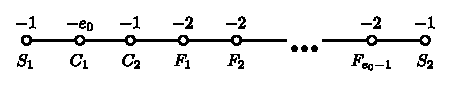
\includegraphics[scale=1.2]{figures/chap2-fig34.eps}
\end{figure}

\item Assume that $d_{0}>1$. Then we have:
$$
\Gamma=d_{0}C_{1}+e_{0}C_{2}+z_{1}+z_{2},
$$
where:
\begin{enumerate}
\renewcommand{\theenumii}{\arabic{enumii}}
\renewcommand{\labelenumii}{\rm\theenumii$^{\circ}$}
\item $Z_{i}$ is an effective divisor such that $\Supp(Z_{i})=R_{i}$
  for $i=1,2$;

\item $(C^{2}_{1})=-(q_{1}+1)$ and $(C^{2}_{2})=-1$;

\item $S_{1}\cup S_{2}\cup \Supp(\Gamma)$ has the weighted graph:
\begin{figure}[H]
\centering
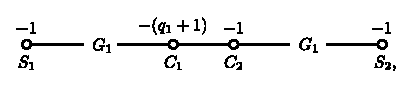
\includegraphics[scale=1.2]{figures/chap2-fig35.eps}
\end{figure}
\noindent
$G_{i}$ being the weighted graph of the irreducible components
contained in $R_{i}$ for $i=1,2$.
\end{enumerate}
\end{enumerate}
\end{lemma*}

A\pageoriginale\ proof will be given in the subparagraphs \ref{chap2:6.17.1}
$\sim$ \ref{chap2:6.17.4} below. The facts which we frequently use in the
course of a proof are the followings: Let $V$ be a nonsingular
projective surface, let $\varphi:V\to \mathbb{P}^{1}_{k}$ be a
surjective morphism whose general fibers are isomorphic to
$\mathbb{P}^{1}_{k}$ and let $\Gamma:=n_{1}C_{1}+\cdots+n_{r}C_{r}$ be
a reducible fiber of $\varphi$. Let $\tau:V\to W$ be a contraction of
several components contained in $\Gamma$, where $W$ is
nonsingular. Then, in the fiber $\tau_{\ast}(\Gamma)$ of the fibration
$\psi:W\to \mathbb{P}^{1}_{k}$ with $\varphi=\psi\cdot\tau$ the
following assertions hold true (\cf Lemma \ref{chap2:2.2}):
\begin{enumerate}
\renewcommand{\theenumi}{\Alph{enumi}}
\renewcommand{\labelenumi}{(\theenumi)}
\item No three distinct components of $\tau_{\ast}(\Gamma)$ have a
  point in common,

\item Let $S$ be a cross-section of $\varphi$. Then no two distinct
  components of $\tau_{\ast}(\Gamma)$ have a point in common on $\tau(S)$.
\end{enumerate}

In each stage of proof where we proceed on {\em reduction ad absurdum},
if we obtain a situation contrary to the assertion (A) (or (B), \resp)
we shall say that we obtain a contradiction of type (A) (or (B),
\resp).

\subsubsection{A proof of the first assertion of the lemma.}\label{chap2:6.17.1}

\begin{enumerate}
\renewcommand{\theenumi}{\Roman{enumi}}
\renewcommand{\labelenumi}{(\theenumi)}
\item Assume that $d_{0}=1$ and $e_{0}>1$. By virtue of Lemma
  \ref{chap2:6.15}, (2), $\Gamma$ has exactly two irreducible components
  $C_{1}$ and $C_{2}$ other than those contained in $R$, one of which,
  say $C_{1}$, has multiplicity $1$ in $\Gamma$ and intersects $S_{1}$
  transversely. Since $\Gamma\cap U$ is connected, $C_{1}$ and
  $C_{2}$ intersect each other in a single point on $U$. Then
  $C_{1}\cap R=\phi$ and $C_{2}$ intersects some component $T$ in
  $R$. Since those components contained in $R$ are not exceptional
  components of $\Gamma$, either\pageoriginale\ one of $C_{1}$ and
  $C_{2}$ is an exceptional component. We shall show that $C_{2}$ is
  so. Indeed, if $C_{1}$ is an exceptional component, so is $C_{2}$ by
  virtue of Lemma \ref{chap2:2.2}, (6).

\item We shall show that $T=F_{1}$. Suppose that $T=F_{i}(i\neq 1,
  e_{0}-1)$. Then since $(T^{2})=-2$ three components $\tau(C_{1})$,
  $\tau(F_{i-1})$ and $\tau(F_{i+1})$ of $\tau_{\ast}\Gamma$ have a
  point in common after the contraction $\tau$ of $C_{1}$ and $T$,
  which is a contradiction of type (A). If $T=F_{e_{0}-1}$ and
  $e_{0}>2$ then two components $\tau(C_{1})$ and $\tau(F_{e_{0}-2})$
  have a point in common on $\tau(S_{2})$ after the contraction $\tau$
  of $C_{2}$ and $T$, which is a contradiction of type (B). Hence
  $T=F_{1}$ and $S_{1}\cup S_{2}U\Supp(\Gamma)$ has the weighted graph
  as given in the statement, where $(C^{2}_{0})=-e_{0}$ because
  $C_{1}$ has self-intersection multiplicity $0$ after the contraction
  of $C_{2},F_{1},\ldots,F_{e_{0}-1}$. Once we know the way of
  contracting $\Gamma$ to a single (irreducible) curve, it is an easy
  task to write down $\Gamma$ in the form as given in the statement.
\end{enumerate}

\subsubsection{}\label{chap2:6.17.2}
In the remaining of the paragraph \ref{chap2:6.17} we assume that
$d_{0}>1$. By virtue of Lemma \ref{chap2:6.15}, (2) and the proof of
Lemma \ref{chap2:6.16} we know that $\Gamma$ has exactly two irreducible
components $C_{1}$ and $C_{2}$ other than those contained in
$R_{1}\cup R_{2}$ such that $C_{1}$ and $C_{2}$ intersect each other
transversely in a single point on $U$ and that $C_{i}\cap R_{i}\neq
\phi(i=1,2)$, $C_{1}\cap R_{2}=\phi$ and $C_{2}\cap R_{1}=\phi$. Let
$T_{i}$ be a unique irreducible component of $R_{i}$ such that
$(R_{i}\cdot C_{i})>0$ for $i=1,2$. Let $G_{i}$ be the weighted graph
of $R_{i}$ for $i=1,2$. Note that for $i=1,2,R_{i}\neq \phi$ and
$R_{i}$ contains no exceptional components. This implies that either
one of $C_{1}$ and $C_{2}$ is an exceptional\pageoriginale\ component,
\iec $(C^{2}_{1})=-1$ or $(C^{2}_{2})=-1$. We shall show that
$T_{1}=E(1,1)$ and $T_{2}=F(1,1)$. In order to do so we shall consider
several possible cases separately. To avoid the tedious lengthiness a
proof will not exceed a sketchy one.

\paragraph{The case where $T_{1}$ and $T_{2}$ are non-terminal
  components in the graphs $G_{1}$ and $G_{2}$, respectively.}\label{chap2:6.17.2.1}


Let $D_{1}$ and $D'_{1}$ (or, $D_{2}$ and $D'_{2}$, \resp) be
components in $R_{1}$ (or $R_{2}$, \resp) which are linked to $T_{1}$
(or $T_{2}$, \resp) in the graph $G_{1}$ (or $G_{2}$, \resp). Then we
have the configuration as follows:
\begin{figure}[H]
\centering
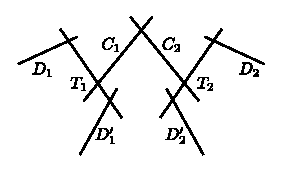
\includegraphics[scale=1.2]{figures/chap2-fig36.eps}
\end{figure}

Suppose that $(C^{2}_{1})=-1$. Then either one of $T_{1}$ and $C_{2}$
becomes contractible after contracting $C_{1}$, \iec $(T^{2}_{1})=-2$
or $(C^{2}_{2})=-2$. If $T_{1}$ is so the contraction $\tau$ of
$C_{1}$ and $T_{1}$ gives out three components $\tau(D_{1})$,
$\tau(D'_{1})$ and $\tau(C_{2})$ of $\tau_{\ast}(\Gamma)$ having a
point in common, a contradiction of type (A). If $(C^{2}_{2})=-2$ then
either one of $T_{1}$ and $T_{2}$ becomes contractible after
contracting $C_{1}$ and $C_{2}$, \iec $(T^{2}_{1})=-3$ or
$(T^{2}_{2})=-2$. If $(T^{2}_{1})=-3$ the contraction of $C_{1}$,
$C_{2}$ and $T_{1}$ leads us to a contradiction of type (A). If
$(T^{2}_{2})=-2$ the contraction of $C_{1}$, $C_{2}$ and $T_{2}$ leads
us to a contradiction of type (A). Thus the assumption
$(C^{2}_{1})=-1$ ends up with a contradiction.\pageoriginale\
Similarly, we can show the impossibility of the assumption
$(C^{2}_{2})=-1$. 

\paragraph{The case where $T_{1}$ is a terminal component in the graph
$G_{1}$ and $T_{2}$ is a non-terminal component in the graph $G_{2}$.}\label{chap2:6.17.2.2}

Let $D_{2}$ and $D'_{2}$ be as in \ref{chap2:6.17.2.1}.
\begin{enumerate}
\renewcommand{\theenumi}{\Roman{enumi}}
\renewcommand{\labelenumi}{(\theenumi)}
\item Firstly we shall consider the case $m=1$. Then $R_{1}\cup S_{1}$
  and $R_{2}\cup S_{2}$ have the following weighted graphs (\cf
  \ref{chap2:6.10} and \ref{chap2:6.13.4}):
\begin{figure}[H]
\centering
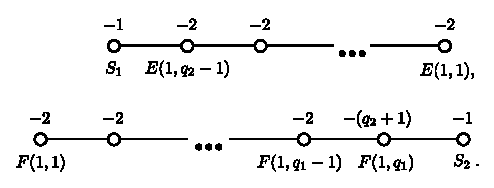
\includegraphics[scale=1.2]{figures/chap2-fig37.eps}
\end{figure}

Hence $(T^{2}_{2})=-2$. If $(C^{2}_{2})=-1$ then the contraction
$\tau$ of $C_{2}$ and $T_{2}$ turns out three components
$\tau(D_{2})$, $\tau(D'_{2})$ and $\tau(C_{1})$ of
$\tau_{\ast}(\Gamma)$ having a point in common, a contradiction of
type $(A)$. Hence $(C^{2}_{2})\neq -1$ and $(C^{2}_{1})=-1$. Then
$T_{1}=E(1,1)$. Indeed, if $T_{1}=E(1,q_{2}-1)$ and $q_{2}\geqq 3$
then the contraction $\tau$ of $C_{1}$ and $T_{2}$ gives out two
components $\tau(C_{2})$ and $\tau(E(1,q_{2}-2))$ of
$\tau_{\ast}(\Gamma)$ having a point in common on $\tau(S_{1})$, a
contradiction of type (B). Since $C_{2}$ becomes contractible after
the contraction of $C_{1}$, $E(1,1),\ldots,E(1,q_{2}-1)$ we have
$(C^{2}_{2})=-(q_{2}+1)$. Then by the contraction $\tau$ of $C_{1}$,
$E(1,1),\ldots,E(1,q_{2}-1)$, $C_{2}$ and $T_{2}$ we have two
components $\tau(D_{2})$ and $\tau(D'_{2})$ of $\tau_{\ast}(\Gamma)$
possessing a point in common on $\tau(S_{1})$, a contradiction of type
(B). Thus, this case is impossible. 

\item Now\pageoriginale\ we assume that $m>1$. Looking into the graph
  of $G_{1}$ which is the subgraph of $\mathscr{E}$ (\cf Figure 2 of
  \ref{chap2:6.10}) consisting of components $E(i,j)$'s between $E(1,1)$ and
  $E(m,p_{m})$ (with $E(m,p_{m})$ excluded) we know that the
  contraction of all possible components in $C_{1}\cup R_{1}$ cannot
  reduce $C_{1}\cup R_{1}$ to a point. Let
  $D^{(1)}_{1},\ldots,D^{(r-1)}_{1}$ and $D^{(r)}_{1}(r\geqq 1)$ be
  the components in $R_{1}$ such that:
\begin{enumerate}
\renewcommand{\theenumii}{\arabic{enumii}}
\renewcommand{\labelenumii}{\rm\theenumii$^{\circ}$}
\item $T_{1}=D^{(1)}_{1}$, and $D^{(i)}_{1}$ is linked to
  $D_{1}^{(i+1)}$ in the graph $G_{1}$ for $1\leqq i\leqq r-1$,

\item $((D^{(i)}_{1})^{2})=-2$ if $i<r$ and $((D^{(r)}_{1})^{2})\neq -2$.
\end{enumerate}
Suppose that $(C^{2}_{2})=-1$. Then we have either $(T^{2}_{2})=-2$ or
$(C^{2}_{1})=-2$. If $(T^{2}_{2})=-2$ the contraction of $C_{2}$ and
$T_{2}$ leads us to a contradiction of type (A). If $(C^{2}_{1})=-2$
then $T_{2}$ becomes contractible after the contraction of
$C_{2},C_{1},D^{(1)}_{1},\ldots,D_{1}^{(r-1)}$, \iec
$(T^{2}_{2})=-(r+2)$. The contraction $\tau$ of
$C_{2},C_{1},D^{(1)}_{1},\ldots,D^{(r-1)}_{1}$ and $T_{2}$ gives out
three components $\tau(D_{2}),\tau(D'_{2})$ and $\tau(D^{(r)}_{1})$ of
$\tau_{\ast}(\Gamma)$ having a point in common, a contradiction of
type (A). Hence $(C^{2}_{2})\neq -1$ and $(C^{2}_{1})=-1$.

\item We shall show that $T_{1}=E(1,1)$. Indeed, assume the contrary:
  $T_{1}\neq E(1,1)$. If $r\geqq 2$ then the contraction $\tau$ of
  $C_{1}$ and $D_{1}^{(1)}$ gives out two components
  $\tau(D^{(2)}_{1})$ and $\tau(C_{2})$ of $\tau_{\ast}(\Gamma)$
  having a point in common on $\tau(S_{1})$, a contradiction of type
  (B). Hence $r=1$, $(C^{2}_{2})=-2$ and either $(T^{2}_{1})=-3$
  (where $T_{1}=D_{1}^{(r)}$) or $(T^{2}_{2})=-2$. If $(T^{2}_{2})=-2$
  then the contraction of $C_{1}$, $C_{2}$ and $T_{2}$ leads us to a
  contradiction of type (A). If $(T^{2}_{1})=-3$ and $R_{1}$ contains
  at least two components (\iec $R_{1}$ has a component $D'_{1}$ such
  that $D'_{1}\neq T_{1}$ and $(D'_{1}\cdot T_{1})=1$) then the
  contraction $\tau$ of $C_{1}$, $C_{2}$ and $T_{1}$\pageoriginale\
  gives out two components $\tau(D'_{1})$ and $\tau(T_{2})$ possessing
  a point in common on $\tau(S_{1})$, a contradiction of type (B). The
  only remaining case is: $r=1$, $R_{1}=T_{1}$ and
  $(T^{2}_{1})=-3$. Then $(T^{2}_{2})=-3$. However, the contraction
  $\tau$ of $C_{1}$, $C_{2}$, $T_{1}$ and $T_{2}$ gives out two
  components $\tau(D_{2})$ and $\tau(D'_{2})$ having a point in common
  on $\tau(S_{1})$, a contradiction of type (B). Therefore,
  $T_{1}=E(1,1)$.

\item $C_{2}$ becomes contractible by contracting $C_{1}$,
  $D^{(1)}_{1},\ldots,D_{1}^{(r-1)}$ and either one of $D^{(r)}_{1}$
  and $T_{2}$ becomes contractible by contracting $C_{2}$ further. If
  this is $T_{2}$ the contraction of $C_{1}$,
  $D^{(1)}_{1},\ldots,D^{(r-1)}_{1}$, $C_{2}$ and $T_{2}$ turns out a
  contradiction of type (A). If this is $D^{(r)}_{1}$ and if there
  exists a sequence of components
  $D^{(r+1)}_{1},\ldots,D^{(t-1)}_{1},D^{(t)}_{1}$ in $R_{1}$ such
  that $D^{(i)}_{1}$ is linked to $D^{(i+1)}_{1}$ for $r\leqq i\leqq
  t-1$ and that $((D^{(i)}_{1})^{2})=-2$ if $r<i<t$ and
  $((D^{(t)}_{1})^{2})\neq -2$ then $T_{2}$ becomes contractible after
  the contraction of
  $C_{1},D^{(1)}_{1},\ldots,D^{(r-1)}_{1},C_{2},D^{(r)}_{1},\ldots,D^{(t-1)}_{1}$,
  while we obtain a contradiction of type (A) by contracting $T_{2}$
  further. The remaining cases are the next two: (1) $m=2$ and
  $p_{2}=2$, or (2) $m=3$ and $p_{2}=1$. In each of the cases we have
  the following weighted graphs of $S_{1}\cup R_{1}\cup C_{1}\cup
  C_{2}$ and $S_{2}\cup R_{2}$:
\end{enumerate}

(1)~
\vskip -.8cm

\begin{figure}[H]
\hspace{2cm}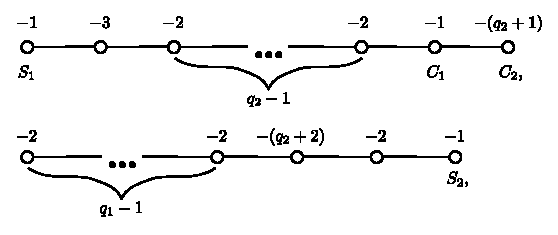
\includegraphics{figures/chap2-fig38.eps}
\end{figure}

(2)~
\vskip -.9cm

\begin{figure}[H]
\hspace{2cm}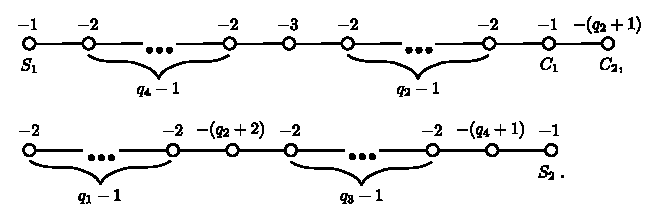
\includegraphics[scale=.85]{figures/chap2-fig39.eps}
\end{figure}
\pageoriginale\

However, it is easy to see that both cases end up with
contradictions. Thus, this case is impossible.

\paragraph{The case where $T_{1}$ is a non-terminal component in
  the graph $G_{1}$ and $T_{2}$ is a terminal component in the graph
  $G_{2}$.}\label{chap2:6.17.2.3} 

The same arguments as in \ref{chap2:6.17.2.2} with slight modifications show
that this case is impossible. The details are left to the readers.

\paragraph{The case where both $T_{1}$ and $T_{2}$ are terminal
  components in the graphs $G_{1}$ and $G_{2}$,
  respectively.}\label{chap2:6.17.2.4}

We shall show that $T_{1}=E(1,1)$ and $T_{2}=F(1,1)$.
\begin{enumerate}
\renewcommand{\theenumi}{\Roman{enumi}}
\renewcommand{\labelenumi}{(\theenumi)}
\item We shall first show that $T_{1}=E(1,1)$. Assume the
  contrary. Then $R_{1}$ has at least two components. Suppose that
  $(C^{2}_{1})=-1$. Then $(T^{2}_{1})\neq -2$, for otherwise the
  contraction $\tau$ of $C_{1}$ and $T_{1}$ would lead us to a
  contradiction of type (B). Hence $(C^{2}_{2})=-2$. Let
  $D^{(1)}_{2},\ldots,D^{(s)}_{2}(s\geqq 1)$ be the components of
  $R_{2}$ such that:
\begin{enumerate}
\renewcommand{\theenumii}{\arabic{enumii}}
\renewcommand{\labelenumii}{\rm(\theenumii)}
\item $T_{2}=D^{(1)}_{2}$, and $D^{(i)}_{2}$ is linked to
  $D^{(i+1)}_{2}$ in the graph $G_{2}$ for $1\leqq i\leqq s-1$;

\item $((D^{(i)}_{2})^{2})=-2$ for $i<s$ and $((D^{(s)}_{2})^{2})\neq -2$.
\end{enumerate}
[It\pageoriginale\ is easy to ascertain the existence of such
  components by looking into the graph $G_{2}$.] Then $T_{1}$ becomes
contractible after the contraction of $C_{1}$, $C_{2}$,
$D^{(1)}_{2},\ldots,D_{2}^{(s-1)}$, though we reach to a contradiction
of type (B) by contracting $T_{1}$ further. Hence $(C^{2}_{1})\neq -1$
and $(C^{2}_{2})=-1$. Let $D^{(1)}_{2},\ldots,D^{(s)}_{2}$ be as
above. Then $C_{1}$ becomes contractible by contracting
$C_{2},D^{(1)}_{2},\ldots,D^{(s-1)}_{2}$ and either one of $T_{1}$ and
$D^{(s)}_{2}$ becomes contractible by contracting $C_{1}$ further. If
$T_{1}$ is so then we obtain a contradiction of type (B) by
contracting $C_{2},D^{(1)}_{2},\ldots,D^{(s-1)}_{2},C_{1}$ and
$T_{1}$. If $D^{(s)}_{2}$ is so and if there exists a sequence of
components $D^{(s+1)}_{2},\ldots,D^{(u)}_{2}$ in $R_{2}$ such that
$D^{(i)}_{2}$ is linked to $D^{(i+1)}_{2}$ for $s\leqq i\leqq u-1$ and
that $((D^{(i)}_{2})^{2})=-2$ if $s<i<u$ and $((D^{(u)}_{2})^{2})\neq
-2$ then $T_{1}$ becomes contractible by contracting $C_{2}$,
$D^{(1)}_{2},\ldots,D_{2}^{(s-1)},C_{1},D^{(s)}_{2},\ldots,D_{2}^{(u-1)}$,
though we obtain a contradiction of type (B) by contracting $T_{1}$
further. The remaining cases are the next two: (1) $n=2$ and $q_{2}=2$
or (2) $n=3$ and $q_{1}=1$. However, $R_{1}$ consists of only one
components in both cases (\cf \ref{chap2:6.10} and \ref{chap2:6.13.4}), a
contradiction. Hence $T_{1}=E(1,1)$.

\item We shall next show that $T_{2}=F(1,1)$. Assume the contrary:
  $T_{2}\neq F(1,1)$. We shall treat the case $m=1$ first. If $m=1$
  the weighted graph of $\Supp(\Gamma)$ is given as follows:
\begin{figure}[H]
\centering
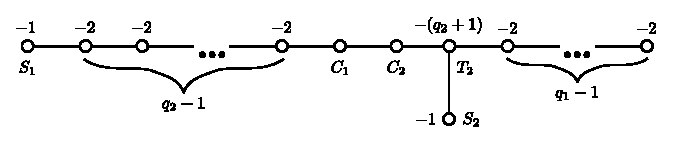
\includegraphics[scale=.95]{figures/chap2-fig40.eps}
\end{figure}
where $q_{2}\geqq 2$. If $(C^{2}_{1})=-1$ then
$(C^{2}_{2})=-(q_{2}+1)$, which is absurd because\pageoriginale\ there
is no contractible components left in $\Gamma$ after $C_{2}$ is
contracted. Hence $(C^{2}_{1})\neq -1$ and $(C^{2}_{2})=-1$. Then
$(C^{2}_{1})=-2$ and $q_{1}=1$, whence $T_{2}=F(1,1)$, a
contradiction. We shall now assume that $m>1$. Suppose that
$(C^{2}_{2})=-1$. Then $(T^{2}_{2})\neq -2$, for otherwise we would
obtain a contradiction of type (B). Hence $(C^{2}_{1})=-2$. Let
$D^{(1)}_{1},\ldots,D^{(r)}_{1}$ be a sequence of components in
$R_{1}$ as in \ref{chap2:6.17.2.2}. Then $T_{2}$ becomes contractible after
contracting $C_{2}$, $C_{1}$, $D^{(1)}_{1},\ldots,D^{(r-1)}_{1}$,
though we obtain a contradiction of type (B) by contracting $T_{2}$
further. Therefore, $(C^{2}_{2})\neq -1$ and $(C^{2}_{1})=-1$. Let
$D^{(1)}_{1},\ldots,D^{(r)}_{1}$ be as above. Then $C_{2}$ becomes
contractible after the contraction of
$C_{1},D^{(1)}_{1},\ldots,D^{(r-1)}_{1}$, and either one of
$D^{(r)}_{1}$ or $T_{2}$ becomes contractible by contracting $C_{2}$
further. If this is $T_{2}$ then we obtain a contradiction of type (B)
because $T_{2}\neq F(1,1)$ implies that $R_{2}$ has at least two
components. If this is $D^{(r)}_{1}$ and if there exists a sequence of
components $D^{(r+1)}_{1},\ldots,D^{(t)}_{1}$ in $R_{1}$ as chosen in
\ref{chap2:6.17.2.2} then $T_{2}$ becomes contractible after contracting
$C_{1},D^{(1)}_{1},\ldots,D^{(r-1)}_{1},C_{2},D^{(r)}_{1},\ldots,D_{1}^{(t-1)}$,
though we obtain a contradiction of type (B) by contracting $T_{2}$
further. The remaining cases are: (1) $m=2$ and $p_{2}=2$, or (2)
$m=3$ and $p_{2}=1$ (\cf the step (IV) of \ref{chap2:6.17.2.2}). These two
cases are easily seen to end up with contradictions. Hence $T_{2}=F(1,1)$.
\end{enumerate}


\subsubsection{}\label{chap2:6.17.3}
By virtue of \ref{chap2:6.17.2} we have the following weighted graph of
$S_{1}\cup S_{2}\cup \Supp(\Gamma)$:
\begin{figure}[H]
\centering
\includegraphics{figures/chap2-fig41.eps}
\end{figure}
If\pageoriginale\ $(C^{2}_{1})=-1$ then
$(C^{2}_{2})=-(q_{2}+1)$. However, by writing down concretely the
weighted graph of $\Supp(\Gamma)$ and performing the contraction of
all possible components of $\Gamma$ we obtain readily a
contradiction. We omit the details. Hence $(C^{2}_{2})=-1$. Again by
writing down concretely the weighted graph of $\Supp(\Gamma)$ we know
that $(C^{2}_{1})=-(q_{1}+1)$ and $\Gamma$ can be, in fact, reduced to
a single (irreducible) component with self-intersection multiplicity
$0$ by contracting all possible components of $\Gamma$.

\subsubsection{}\label{chap2:6.17.4}
The graph $G_{2}$ is written as:
\begin{figure}[H]
\centering
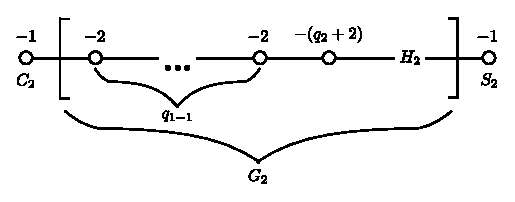
\includegraphics{figures/chap2-fig42.eps}
\end{figure}
Then, looking into the graphs $\mathscr{E}$ and $\mathscr{F}$, we know
that the weighted graph of $\Delta'$ is given by
\begin{figure}[H]
\centering
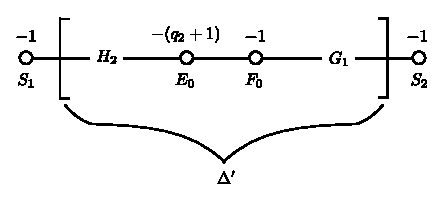
\includegraphics{figures/chap2-fig43.eps}
\end{figure}%raghu
By comparing the weighted graphs of $\Supp(\Gamma)$ and
$\Supp(\Delta')$ we know that the weighted graph of $\Supp(\Delta')$
is obtained from that of $\Supp$ $(\Gamma)$ by contracting $C_{2}$ and
$(q_{1}-1)$ components in $G_{2}$ which are linked successively to
$C_{2}$. Since the multiplicities of $E_{0}$ and $F_{0}$ in $\Delta'$
are $e_{2}$ and $d_{0}=e_{1}$, respectively, we know that
$C_{1}$\pageoriginale\ has multiplicity $d_{0}$ in $\Gamma$ and the
component in $G_{2}$ with weight $-(q_{2}+2)$ has multiplicity $e_{2}$
in $\Gamma$. Then it is apparent that $C_{2}$ has multiplicity
$e_{2}+q_{1}e_{1}=e_{0}$ in $\Gamma$. This completes a proof of Lemma
\ref{chap2:6.17}. 

\subsection{}\label{chap2:6.18}
The ``only if'' part of Theorem \ref{chap2:6.1} is easy to prove. So we
omit a proof. We shall finish this section by noting that if $f$ is as
in the statement then there exists a nontrivial action of the
multiplicative group scheme $G_{m,k}$ on
$\mathbb{A}^{2}_{k}:=\Spec(k[x,y])$ such that $C'_{\alpha}$'s are
$G_{m,k}$-orbits for almost all $\alpha\in k$. Indeed if $f$ is
written as $f:c(x^{d}y^{e}-1)$ we have only to define an action of
$G_{m,k}$ on $\mathbb{A}^{2}_{k}$ via: ${}^{t}x:t^{-e}x$ and
${}^{t}y=t^{d}y$ for $t\in G_{m,k}$.
